\newpage
\section{Thực nghiệm và đánh giá}
\noindent
Chương này trình bày toàn bộ quá trình thực nghiệm của khung dự đoán rủi ro tín dụng dựa trên Causal Machine Learning, được triển khai và đánh giá trên ba bộ dữ liệu tín dụng thực tế với đặc điểm và quy mô khác nhau: Australian Credit Dataset, German Credit Dataset và Lending Club 2007–2014. Bên cạnh việc so sánh hiệu suất phân loại giữa mạng Bayes và các thuật toán máy học cơ sở, chương này còn trình bày chi tiết kết quả của từng giai đoạn trong đường ống xử lý dữ liệu, cấu trúc đồ thị nhân quả học được, cũng như các phân tích diễn giải mô hình thông qua suy luận tiến, suy luận lùi và phân tích kịch bản what-if.

\subsection{Dữ liệu thực nghiệm}
\noindent
Để đánh giá toàn diện hiệu quả của khung dự đoán rủi ro tín dụng dựa trên Causal Machine Learning, nghiên cứu này triển khai thực nghiệm trên ba bộ dữ liệu tín dụng thực tế với quy mô, nguồn gốc và đặc điểm cấu trúc khác nhau, bao gồm Australian Credit Dataset, German Credit Dataset và Lending Club 2007 - 2014. Mỗi bộ dữ liệu đại diện cho một bối cảnh thẩm định tín dụng riêng biệt, từ đó cho phép đánh giá khả năng tổng quát hóa của mô hình trên nhiều loại hình dữ liệu tài chính.

\subsubsection{Mô tả bộ dữ liệu}
Australian Credit Dataset được thu thập từ UCI Machine Learning Repository, phản ánh thông tin hồ sơ tín dụng cá nhân tại Úc với dữ liệu đã được ẩn danh hóa hoàn toàn. Bộ dữ liệu gồm 690 mẫu quan sát và 14 đặc trưng đầu vào sau khi loại bỏ cột mã bưu chính (ZipCode) do không mang giá trị phân biệt rủi ro. Trong số 14 đặc trưng còn lại, 5 biến mang bản chất liên tục gồm Age, Debt, YearsEmployed, CreditScore và Income; 8 biến còn lại là biến phân loại danh nghĩa gồm Gender, BankCustomer, EducationLevel, Ethnicity, CreditHistory, Employed, DriversLicense và Citizen. Phân phối nhãn mục tiêu tương đối cân bằng với 383 mẫu vỡ nợ (55.5\%) và 307 mẫu không vỡ nợ (44.5\%), không tồn tại giá trị khuyết. Bộ dữ liệu được chia theo tỷ lệ 60/40 cho tập huấn luyện và tập kiểm tra.

German Credit Dataset cũng được lấy từ UCI Machine Learning Repository, đại diện cho bài toán phân loại rủi ro tín dụng trong bối cảnh ngân hàng Đức. Bộ dữ liệu gồm 1,000 mẫu quan sát với 20 đặc trưng đầu vào. Trong đó, 3 biến liên tục là month\_duration, credit\_amount và age; 17 biến còn lại là biến phân loại bao gồm status\_account, credit\_history, purpose, status\_savings, years\_employment, status\_and\_sex, secondary\_obligor, collateral, other\_installment\_plans, housing, job, telephone, is\_foreign\_worker và một số biến phụ trợ khác. Nhãn mục tiêu được mã hóa lại từ định dạng chuỗi (``good'' $\rightarrow$ 0, ``bad'' $\rightarrow$ 1), với phân phối 700 mẫu tốt (70\%) và 300 mẫu xấu (30\%), thể hiện sự mất cân bằng lớp ở mức vừa phải. Bộ dữ liệu không có giá trị khuyết và được chia theo tỷ lệ 60/40.

Lending Club 2007-2014 là bộ dữ liệu cho vay ngang hàng quy mô lớn được thu thập từ nền tảng Lending Club, bao gồm 466.345 hồ sơ vay với 151 cột thông tin gốc. Do quy mô và độ phức tạp đặc thù của bộ dữ liệu này, quá trình tiền xử lý đòi hỏi nhiều bước làm sạch chuyên sâu hơn so với hai bộ dữ liệu còn lại. Trước tiên, biến mục tiêu được nhị phân hóa từ cột loan\_status: các trạng thái ``Fully Paid'', ``Current'' và ``Does not meet the credit policy. Status: Fully Paid'' được gán nhãn 0 (không vỡ nợ), trong khi các trạng thái ``Charged Off'', ``Late'', ``In Grace Period'' và ``Does not meet the credit policy. Status: Charged Off'' được gán nhãn 1 (vỡ nợ). Tiếp theo, các cột không mang thông tin thẩm định (id, url, mô tả văn bản) và các cột gây rò rỉ dữ liệu tương lai (total\_pymnt, recoveries, last\_pymnt\_amnt và các biến phản ánh kết quả sau khi giải ngân) bị loại bỏ hoàn toàn. Các cột có tỷ lệ giá trị khuyết vượt quá 50\% cũng bị loại. Trên không gian biến số còn lại, phân tích hệ số phóng đại phương sai (VIF) và lọc tương quan được áp dụng để xử lý đa cộng tuyến, đưa số lượng biến liên tục từ 36 xuống mức tối ưu trước khi đưa vào Lasso. Kết hợp với 10 biến phân loại gồm term, grade, emp\_length, verification\_status, home\_ownership, purpose, addr\_state, initial\_list\_status, hardship\_flag và debt\_settlement\_flag, không gian đặc trưng cuối cùng được xác định. Do giới hạn tài nguyên tính toán khi học cấu trúc mạng Bayes trên tập dữ liệu cực lớn, nghiên cứu lấy mẫu con có kiểm soát với 21,000 mẫu không vỡ nợ và 9,000 mẫu vỡ nợ, tạo thành tập làm việc gồm 30,000 quan sát với tỷ lệ mất cân bằng xấp xỉ 7:3, phản ánh gần đúng phân phối tự nhiên của dữ liệu gốc. Tập này sau đó được chia theo tỷ lệ 60/40 cho huấn luyện và kiểm tra.

Thông tin tổng hợp về ba bộ dữ liệu được trình bày trong Bảng \ref{tab:dataset_summary}.

\begin{table}[htbp]
    \centering
    \caption{Thông tin tổng hợp về các bộ dữ liệu thực nghiệm}
    \label{tab:dataset_summary}
    \renewcommand{\arraystretch}{1.3} % Tăng khoảng cách dòng để bảng thoáng hơn
    \begin{tabular}{|l|c|c|c|c|}
        \hline
        \textbf{Bộ dữ liệu} & \textbf{Số mẫu} & \textbf{Số đặc trưng} & \textbf{Không vỡ nợ} & \textbf{Vỡ nợ} \\ \hline
        Australian & 690 & 14 & 307 & 383 \\ \hline
        German & 1,000 & 20 & 700 & 300 \\ \hline
        Lending Club & 30,000 & 46 & 21,000 & 9,000 \\ \hline
    \end{tabular}
\end{table}

\subsubsection{Phân tích khám phá dữ liệu (EDA)}
\noindent
Trước khi tiến hành xây dựng mô hình, quá trình phân tích khám phá dữ liệu (EDA) được thực hiện trên cả ba bộ dữ liệu nhằm làm rõ đặc điểm phân phối, mức độ mất cân bằng lớp và cấu trúc tương quan giữa các đặc trưng. Kết quả phân tích này đồng thời cung cấp cơ sở thực nghiệm cho các quyết định thiết kế trong đường ống tiền xử lý dữ liệu ở các bước tiếp theo. 

\vspace{1em}
\noindent
\textbf{Mức độ mất cân bằng lớp}

\vspace{0.5em}
\begin{figure}[htbp]
    \centering
    % Hình 1: Australian
    \begin{subfigure}[b]{0.43\textwidth}
        \centering
        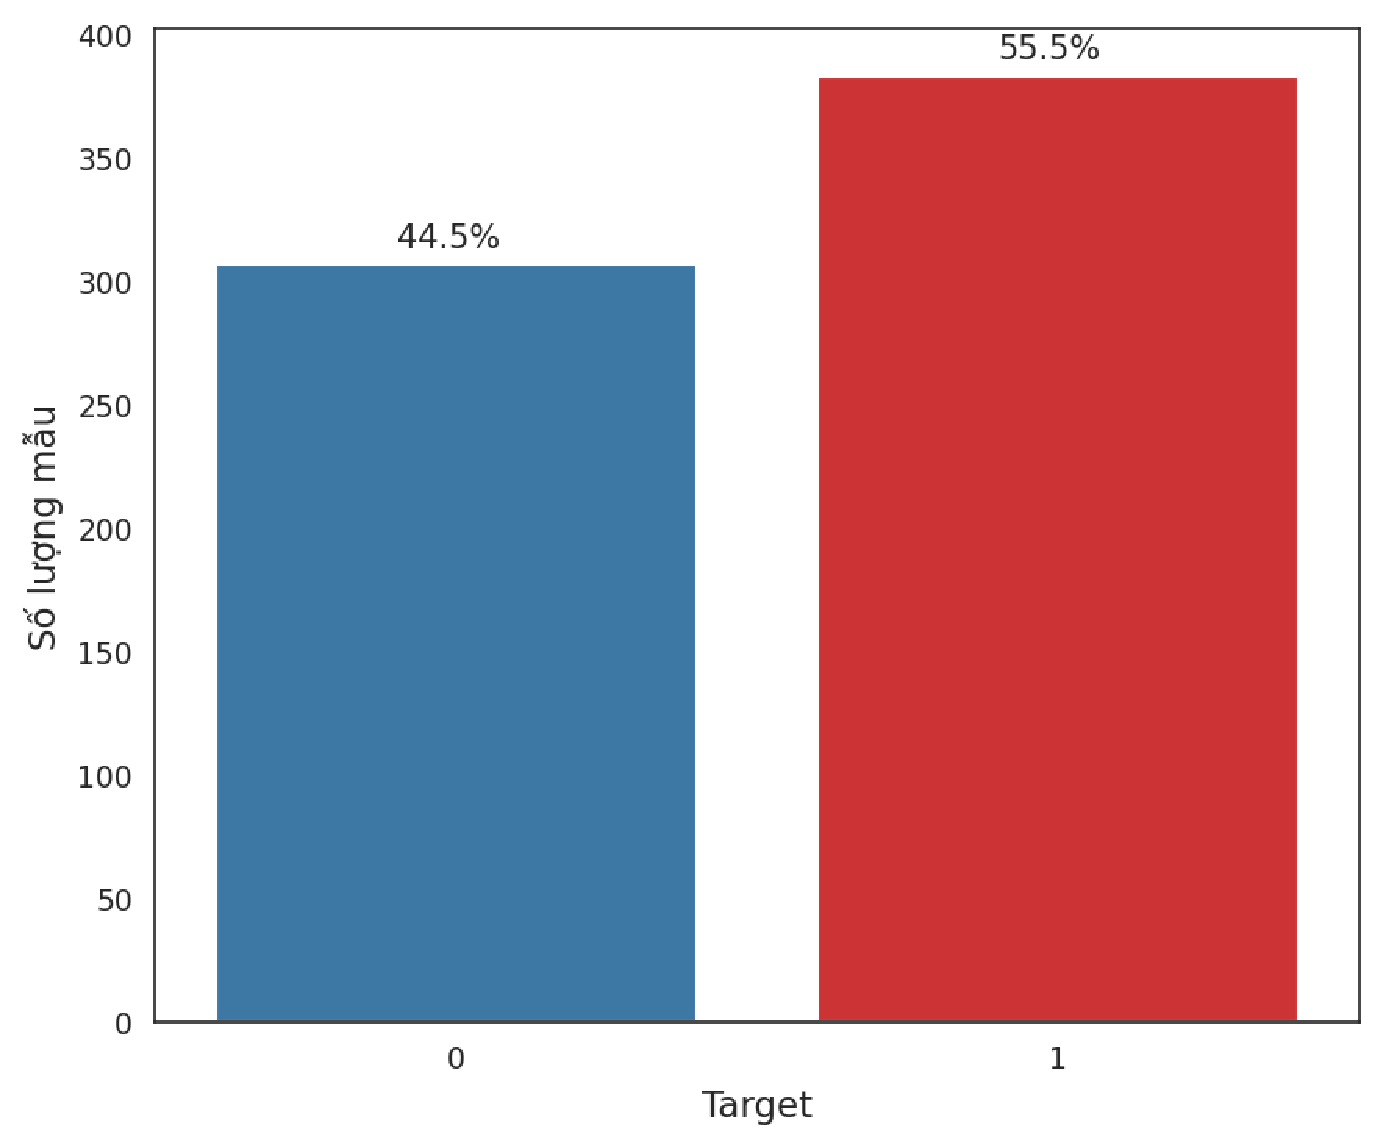
\includegraphics[width=\textwidth]{image/vlz_australian/1_imbalance_au.pdf}
        \caption{Australian Credit}
        \label{fig:imbalance_aus}
    \end{subfigure}
    \hfill
    % Hình 2: German
    \begin{subfigure}[b]{0.43\textwidth}
        \centering
        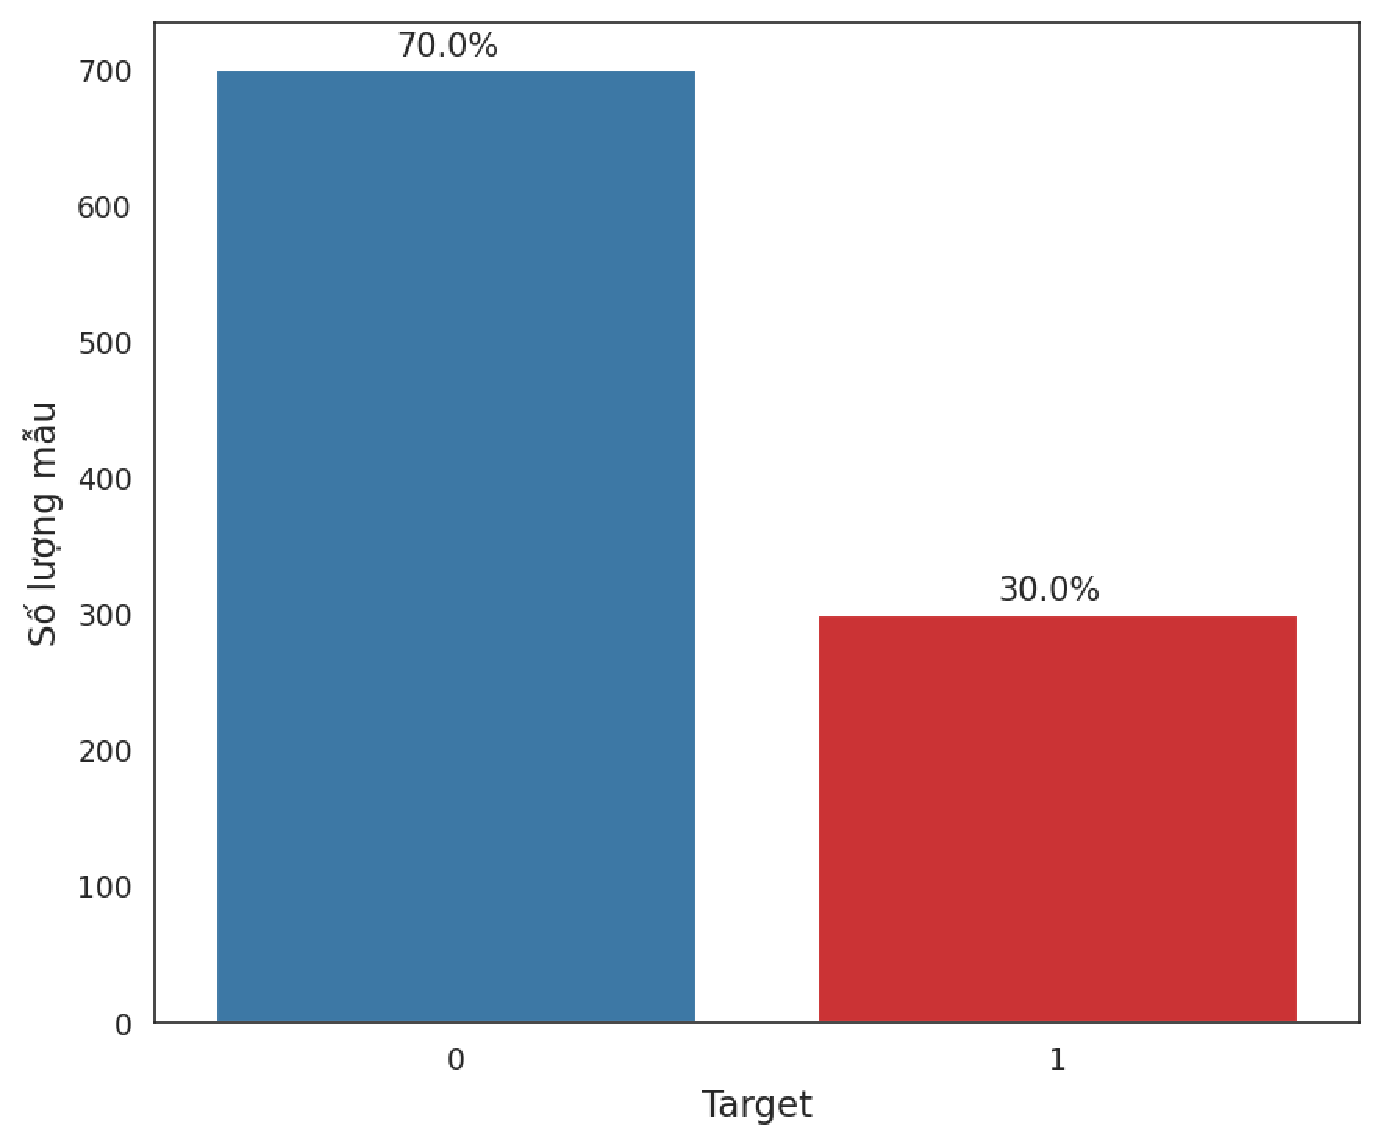
\includegraphics[width=\textwidth]{image/vlz_germany/1_imbalance_ger.pdf}
        \caption{German Credit}
        \label{fig:imbalance_ger}
    \end{subfigure}
    \hfill
    % Hình 3: Lending Club
    \begin{subfigure}[b]{0.43\textwidth}
        \centering
        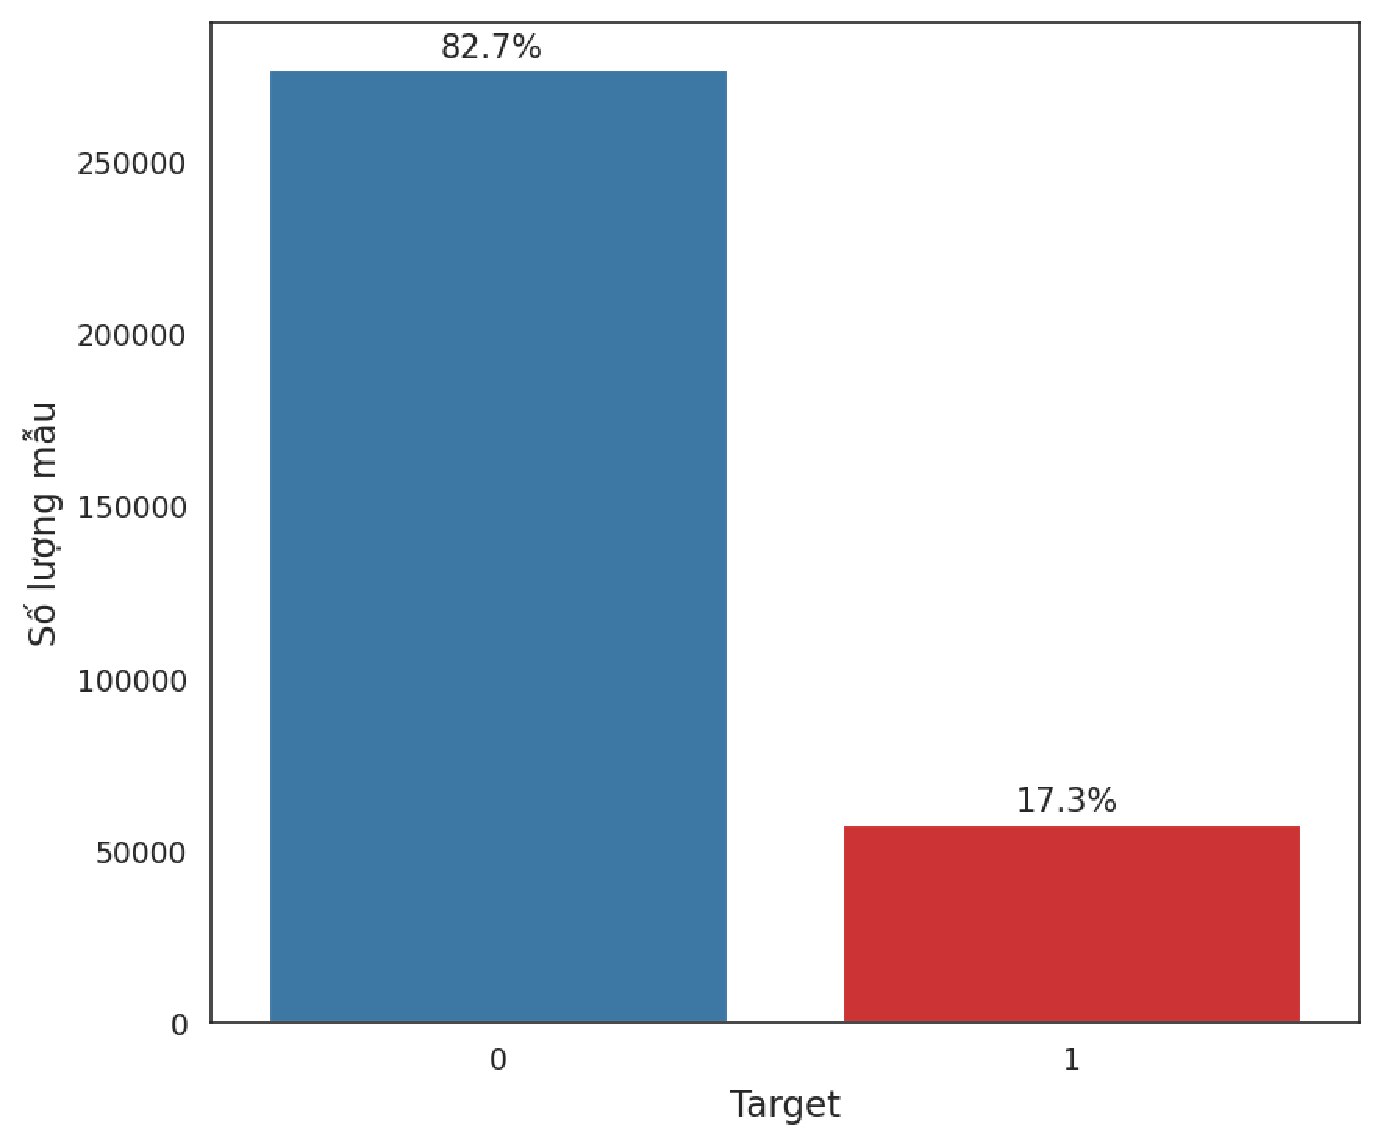
\includegraphics[width=\textwidth]{image/vlz_lending_club/1_imbalance_lend.pdf}
        \caption{Lending Club}
        \label{fig:imbalance_lc}
    \end{subfigure}
    
    \caption{Phân phối nhãn mục tiêu trên ba bộ dữ liệu thực nghiệm}
    \label{fig:class_imbalance}
\end{figure}

\vspace{1em}
Hình \ref{fig:class_imbalance} thể hiện phân phối nhãn mục tiêu của ba bộ dữ liệu. Australian Credit có mức độ cân bằng tốt nhất với tỷ lệ 44.5\% không vỡ nợ và 55.5\% vỡ nợ , gần như đạt cân bằng tự nhiên. German Credit thể hiện sự mất cân bằng vừa phải ở mức 70/30, trong khi tập dữ liệu gốc Lending Club có mức độ mất cân bằng nghiêm trọng nhất với tỷ lệ lên đến 82.7\% không vỡ nợ so với 17.3\% vỡ nợ. Sự chênh lệch này xác nhận sự cần thiết của bước S\_Pro trong đường ống xử lý.

\vspace{1em}
\noindent
\textbf{Phân phối biến liên tục}

Trên bộ dữ liệu Australian (Hình \ref{fig:con_dist_australian}), \texttt{Income} thể hiện phân phối lệch phải cực mạnh. Sau biến đổi $\log(\text{Income} + 1)$, nhóm vỡ nợ tập trung áp đảo ở vùng giá trị rất thấp, trong khi nhóm không vỡ nợ lại phân tán đều hơn và chiếm ưu thế rõ rệt ở các mức thu nhập trung bình và cao. \texttt{Age} tập trung chủ yếu trong độ tuổi 18--35, với nhóm vỡ nợ có xu hướng trẻ hơn, còn nhóm không vỡ nợ mới là nhóm có xu hướng lớn tuổi hơn, thể hiện qua phần đuôi phân phối kéo dài về phía 45--60 tuổi. \texttt{Debt} và \texttt{YearsEmployed} đều lệch phải mạnh, hai nhóm nhãn chồng lấn đáng kể, cho thấy khả năng phân biệt đơn biến hạn chế. Trên bộ dữ liệu German (Hình \ref{fig:con_dist_german}), \texttt{credit\_amount} lệch phải và tập trung dưới 5,000 DM, nhóm vỡ nợ phân tán ở dải giá trị cao hơn. \texttt{month\_duration} thể hiện phân phối đa đỉnh rõ ràng tại các mốc 12, 24 và 36 tháng, phản ánh thực tế các kỳ hạn vay cố định phổ biến, trong đó nhóm vỡ nợ thiên về thời hạn dài hơn. Trên bộ dữ liệu Lending Club (Hình \ref{fig:con_dist_lending}), \texttt{int\_rate} là biến có sức phân biệt rõ nhất trong số các biến liên tục - đường KDE của nhóm vỡ nợ dịch phải đáng kể so với nhóm không vỡ nợ, phản ánh logic tín dụng rằng người vay rủi ro cao bị áp lãi suất cao hơn. \texttt{fico\_range\_low} cho thấy xu hướng ngược lại: điểm tín dụng của nhóm không vỡ nợ cao hơn một cách nhất quán.

% =========================================================================
% KHỐI HÌNH: PHÂN PHỐI CÁC BIẾN LIÊN TỤC THEO TARGET
% =========================================================================
\begin{figure}[htbp]
    \centering
    \begin{subfigure}[b]{\textwidth}
        \centering
        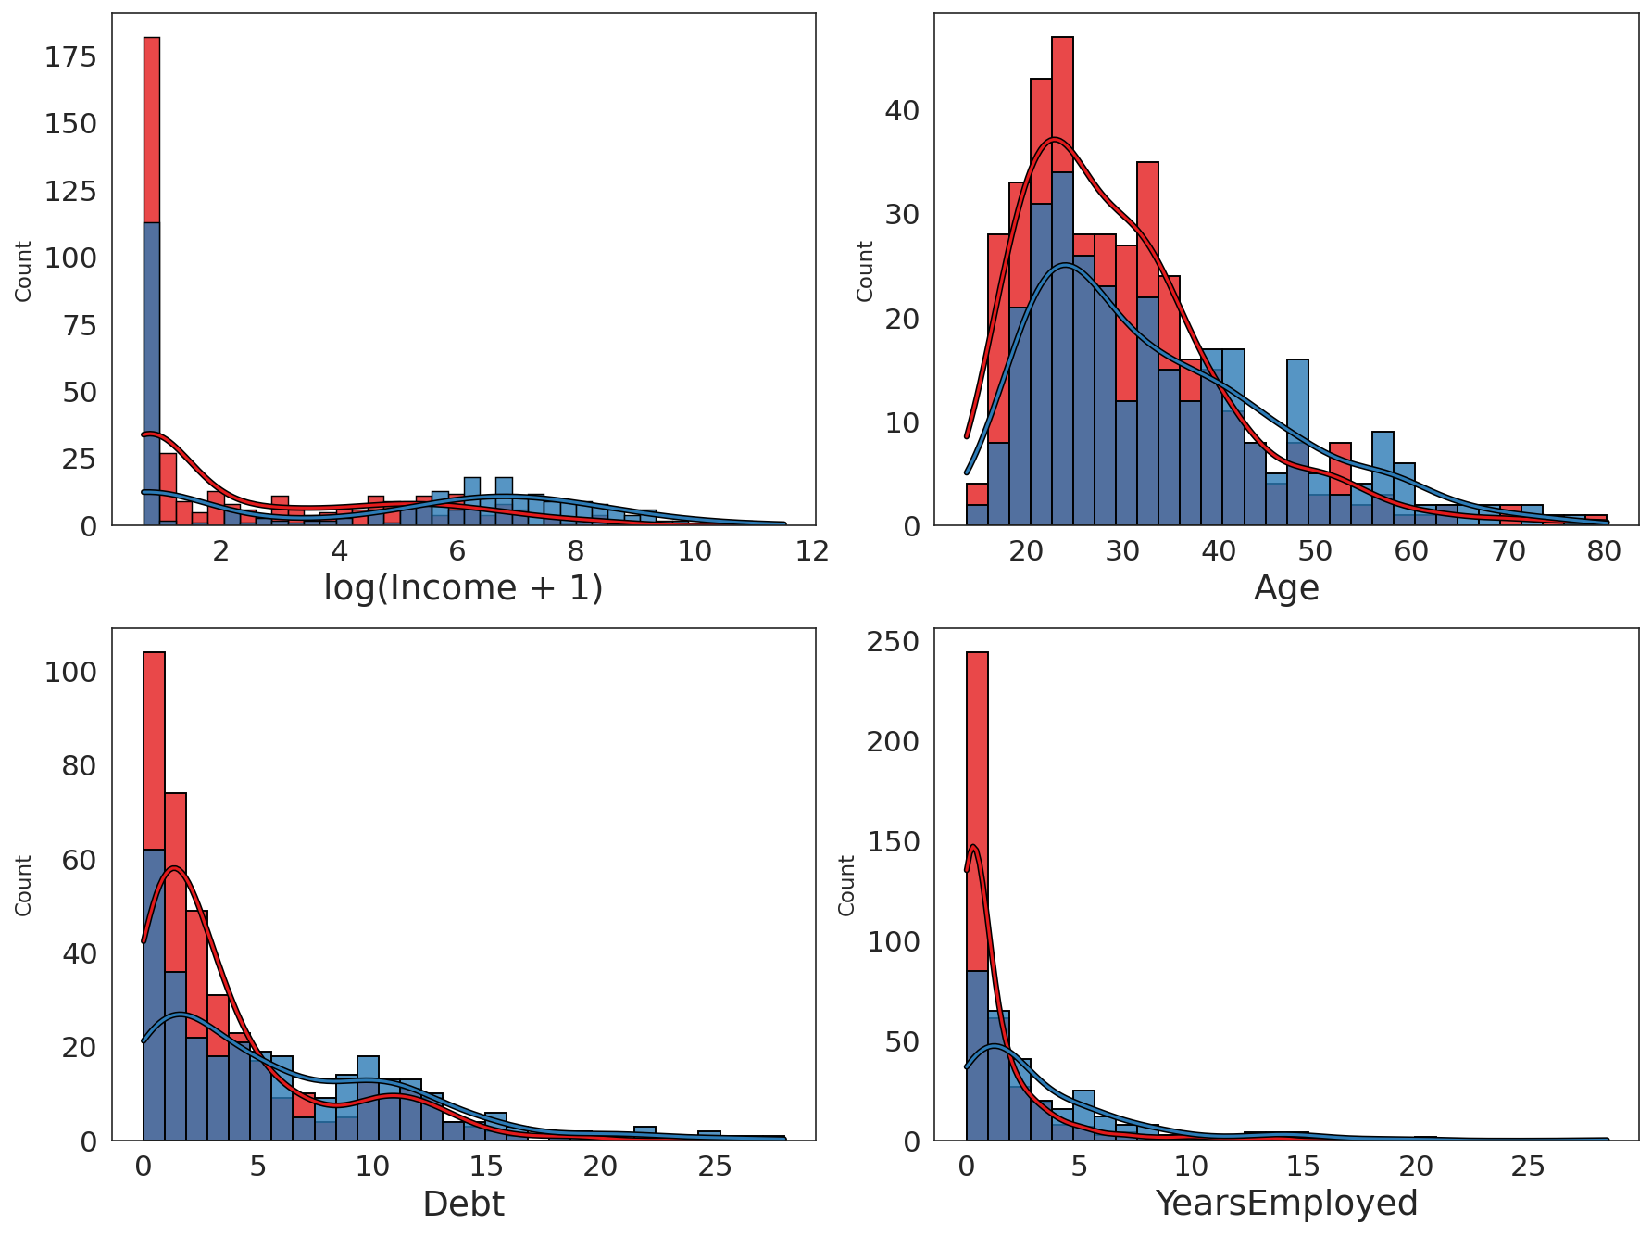
\includegraphics[width=\textwidth]{image/vlz_australian/2_con_dist_au.pdf}
    \end{subfigure}
    
    \caption{Phân phối các biến liên tục theo nhãn \texttt{target} --- Australian Credit. {\newline \small (Trong đó, màu xanh: \texttt{target}~=~0 và màu đỏ: \texttt{target}~=~1)}}
    \label{fig:con_dist_australian}
\end{figure}

\begin{figure}[htbp]
    \centering
    % --- HÀNG 2 ---
    \begin{subfigure}[b]{0.85\textwidth}
        \centering
        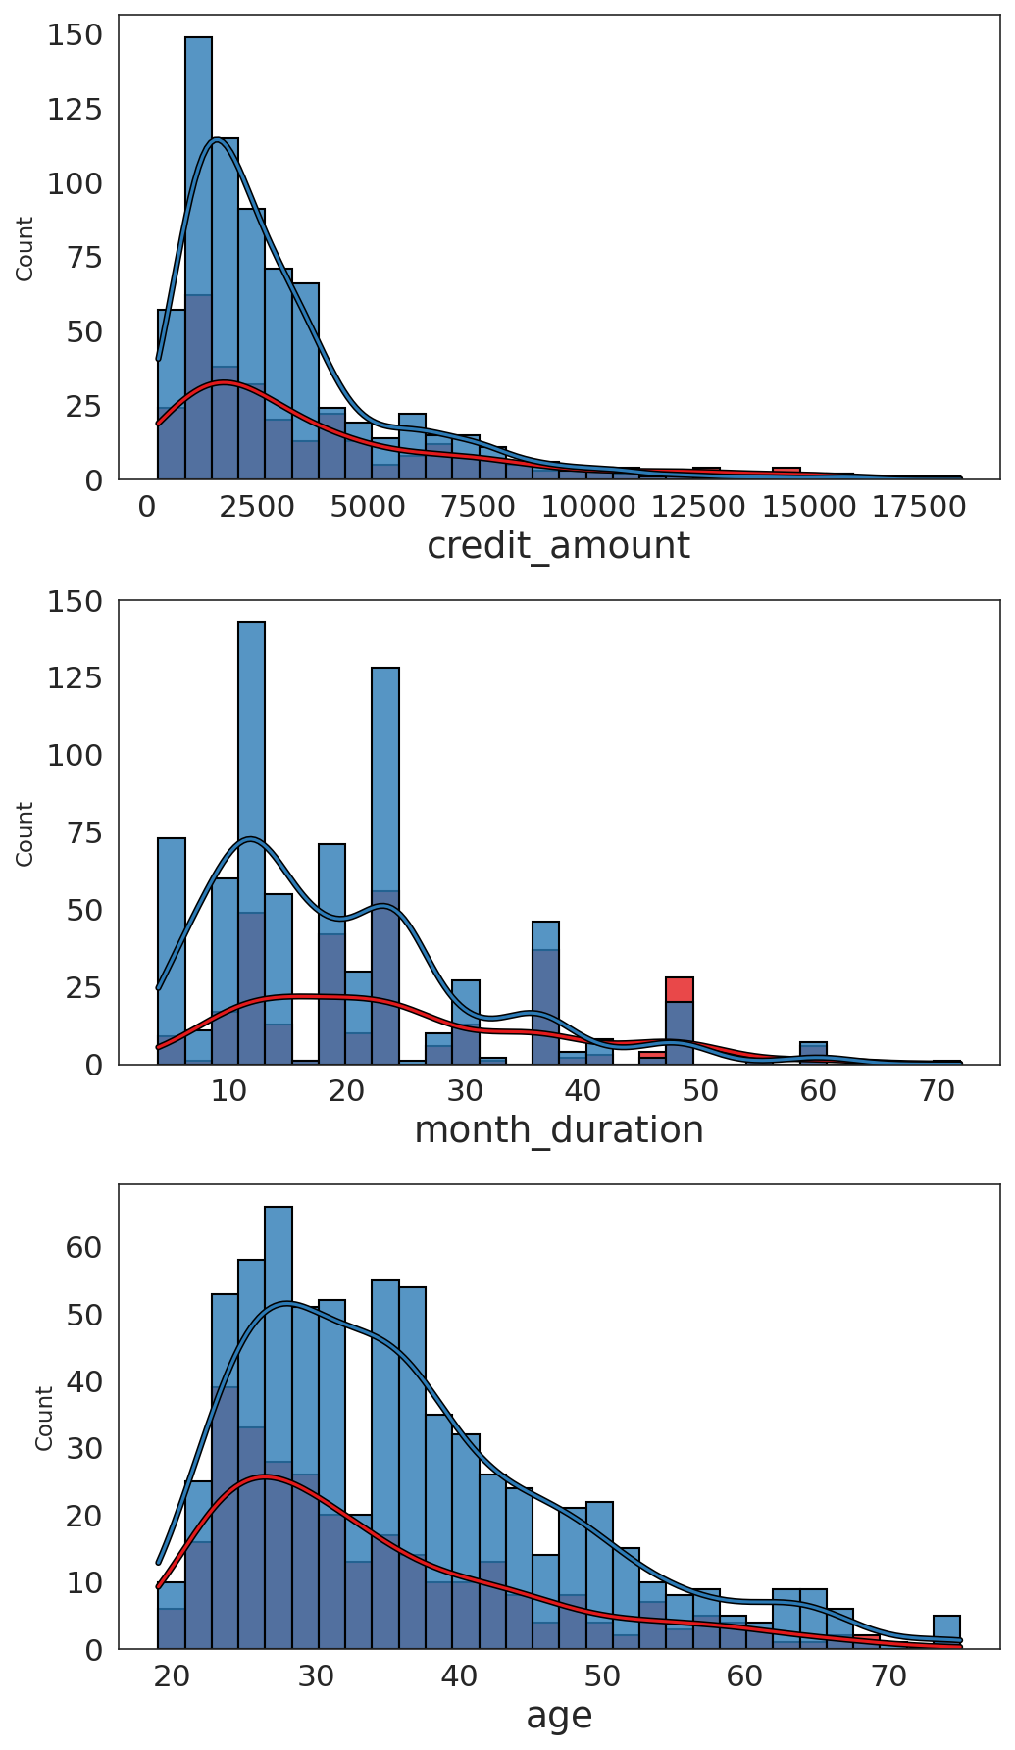
\includegraphics[width=\textwidth]{image/vlz_germany/2_con_dist_ger.pdf}
    \end{subfigure}
    
    \caption{Phân phối các biến liên tục theo nhãn \texttt{target} --- German Credit. {\newline \small (Trong đó, màu xanh: \texttt{target}~=~0 và màu đỏ: \texttt{target}~=~1)}}
    \label{fig:con_dist_german}
\end{figure}

\begin{figure}[htbp]
    \centering
    
    \begin{subfigure}[b]{\textwidth}
        \centering
        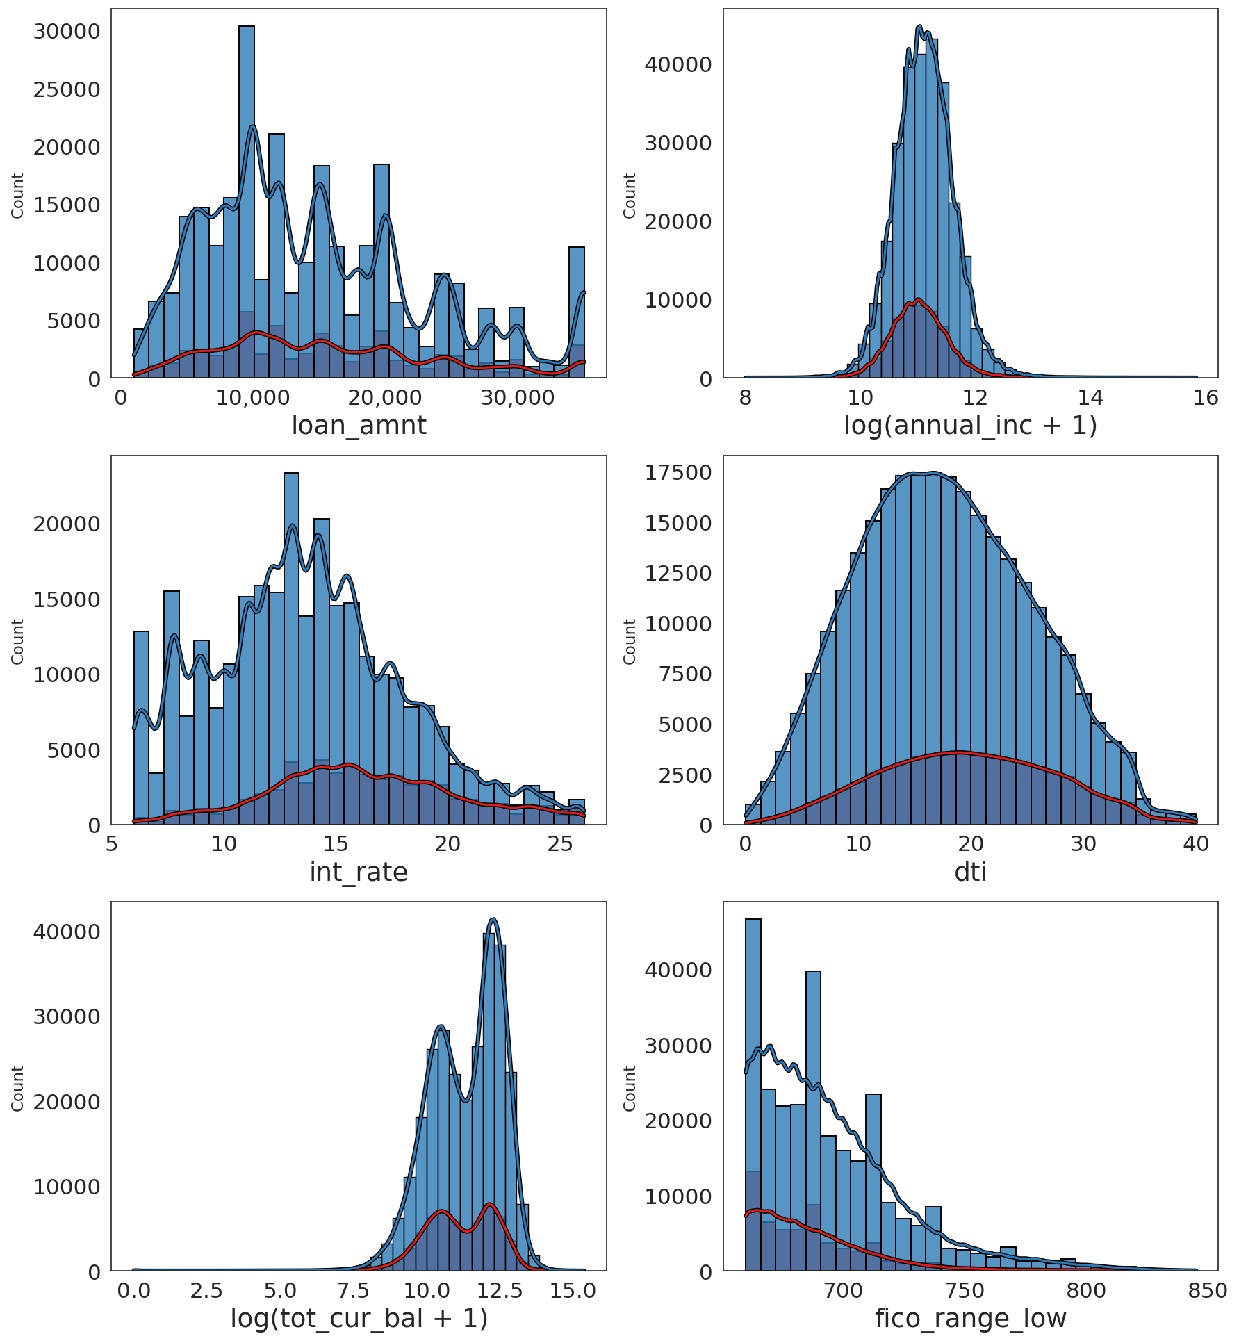
\includegraphics[width=\textwidth]{image/vlz_lending_club/2_con_dist_lend.pdf}
    \end{subfigure}
    
    \caption{Phân phối các biến liên tục theo nhãn \texttt{target} --- Lending Club. {\newline \small (Trong đó, màu xanh: \texttt{target}~=~0 và màu đỏ: \texttt{target}~=~1)}}
    \label{fig:con_dist_lending}
\end{figure}

% =========================================================================
% KHỐI HÌNH: PHÂN PHỐI CÁC BIẾN PHÂN LOẠI THEO TARGET
% =========================================================================
\vspace{0.5em}
\noindent
\textbf{Phân phối biến phân loại} 

Biểu đồ phân phối cho thấy một số biến phân loại có sức phân biệt rủi ro rất rõ ràng. Trên Australian (Hình \ref{fig:cate_dist_australian}), \texttt{CreditHistory} là biến có tính phân biệt cao nhất: nhóm \texttt{CreditHistory} $= 1$ gần như toàn bộ là mẫu không vỡ nợ, trong khi nhóm \texttt{CreditHistory} $= 0$ có tỷ lệ vỡ nợ chiếm ưu thế. \texttt{Employed} cũng thể hiện tính phân biệt tương tự. Trên German (Hình \ref{fig:cate_dist_german}), \texttt{status\_account} là tín hiệu rủi ro mạnh - nhóm không có tài khoản thanh toán (``no checking account'') có tỷ lệ không vỡ nợ áp đảo, trong khi nhóm số dư âm (``$< 0$ DM'') tập trung nhiều mẫu vỡ nợ hơn. \texttt{status\_savings} xác nhận xu hướng tương tự: nhóm tiết kiệm dưới 100 DM chiếm đa số và có tỷ lệ vỡ nợ cao nhất. Trên Lending Club (Hình \ref{fig:cate_dist_lending}), \texttt{grade} là biến phân loại có sức phân biệt mạnh nhất - tỷ lệ vỡ nợ tăng đơn điệu từ hạng A đến G, cho thấy hệ thống xếp hạng nội bộ của Lending Club có tương quan trực tiếp với rủi ro thực tế. Khoản vay 60 tháng cũng có tỷ lệ vỡ nợ cao hơn rõ so với 36 tháng.

\vspace{1.5em}
\begin{figure}[htbp]
    \centering

    \begin{subfigure}[b]{\textwidth}
        \centering
        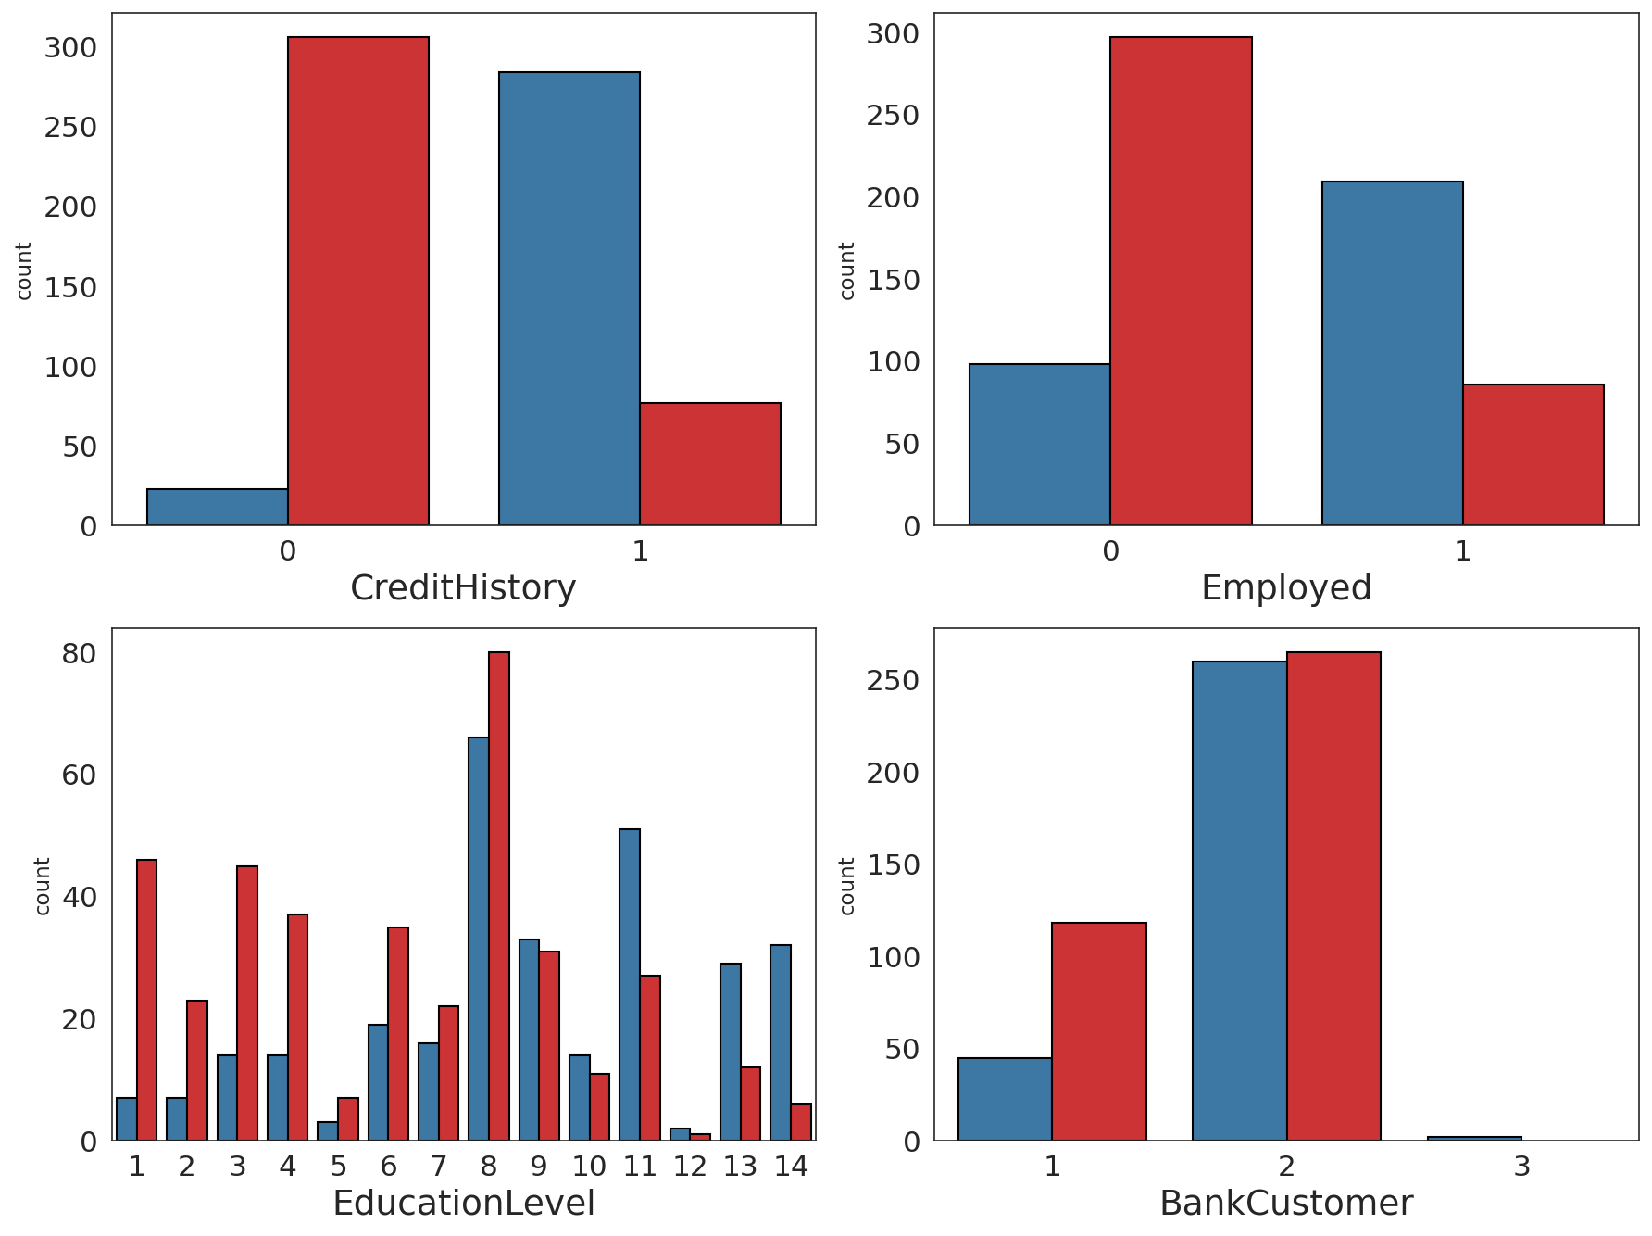
\includegraphics[width=\textwidth]{image/vlz_australian/3_cate_dist_au.pdf}
    \end{subfigure}
    
    \caption{Phân phối các biến phân loại theo nhãn \texttt{target} --- Australian Credit. {\newline \small (Trong đó, màu xanh: \texttt{target}~=~0 và màu đỏ: \texttt{target}~=~1)}}
    \label{fig:cate_dist_australian}
\end{figure}

\begin{figure}[htbp]
    \centering
    
    \begin{subfigure}[b]{\textwidth}
        \centering
        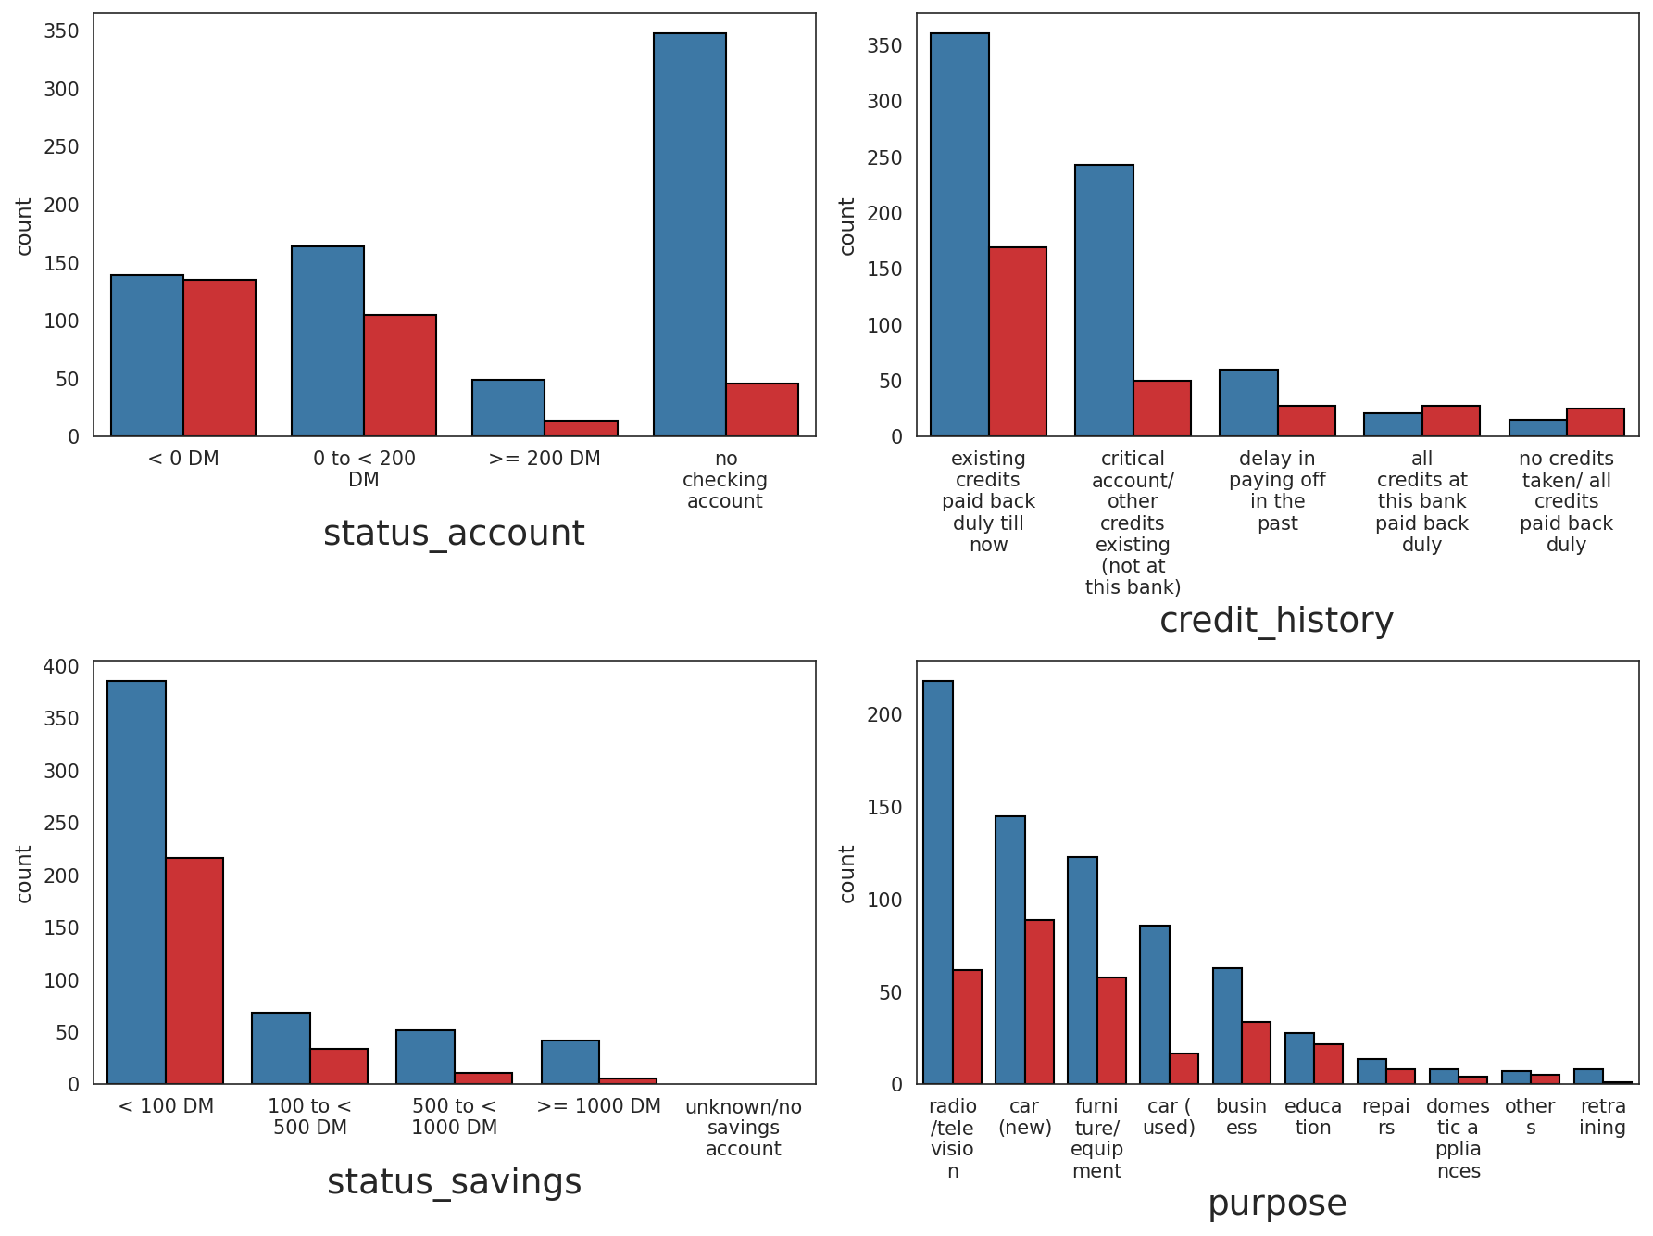
\includegraphics[width=\textwidth,
        height=0.45\textheight]{image/vlz_germany/3_cate_dist_ger.pdf}
    \end{subfigure}
    
    \caption{Phân phối các biến phân loại theo nhãn \texttt{target} --- German Credit. {\newline \small (Trong đó, màu xanh: \texttt{target}~=~0 và màu đỏ: \texttt{target}~=~1)}}
    \label{fig:cate_dist_german}
\end{figure}

\begin{figure}[htbp]
    \centering
    \begin{subfigure}[b]{\textwidth}
        \centering
        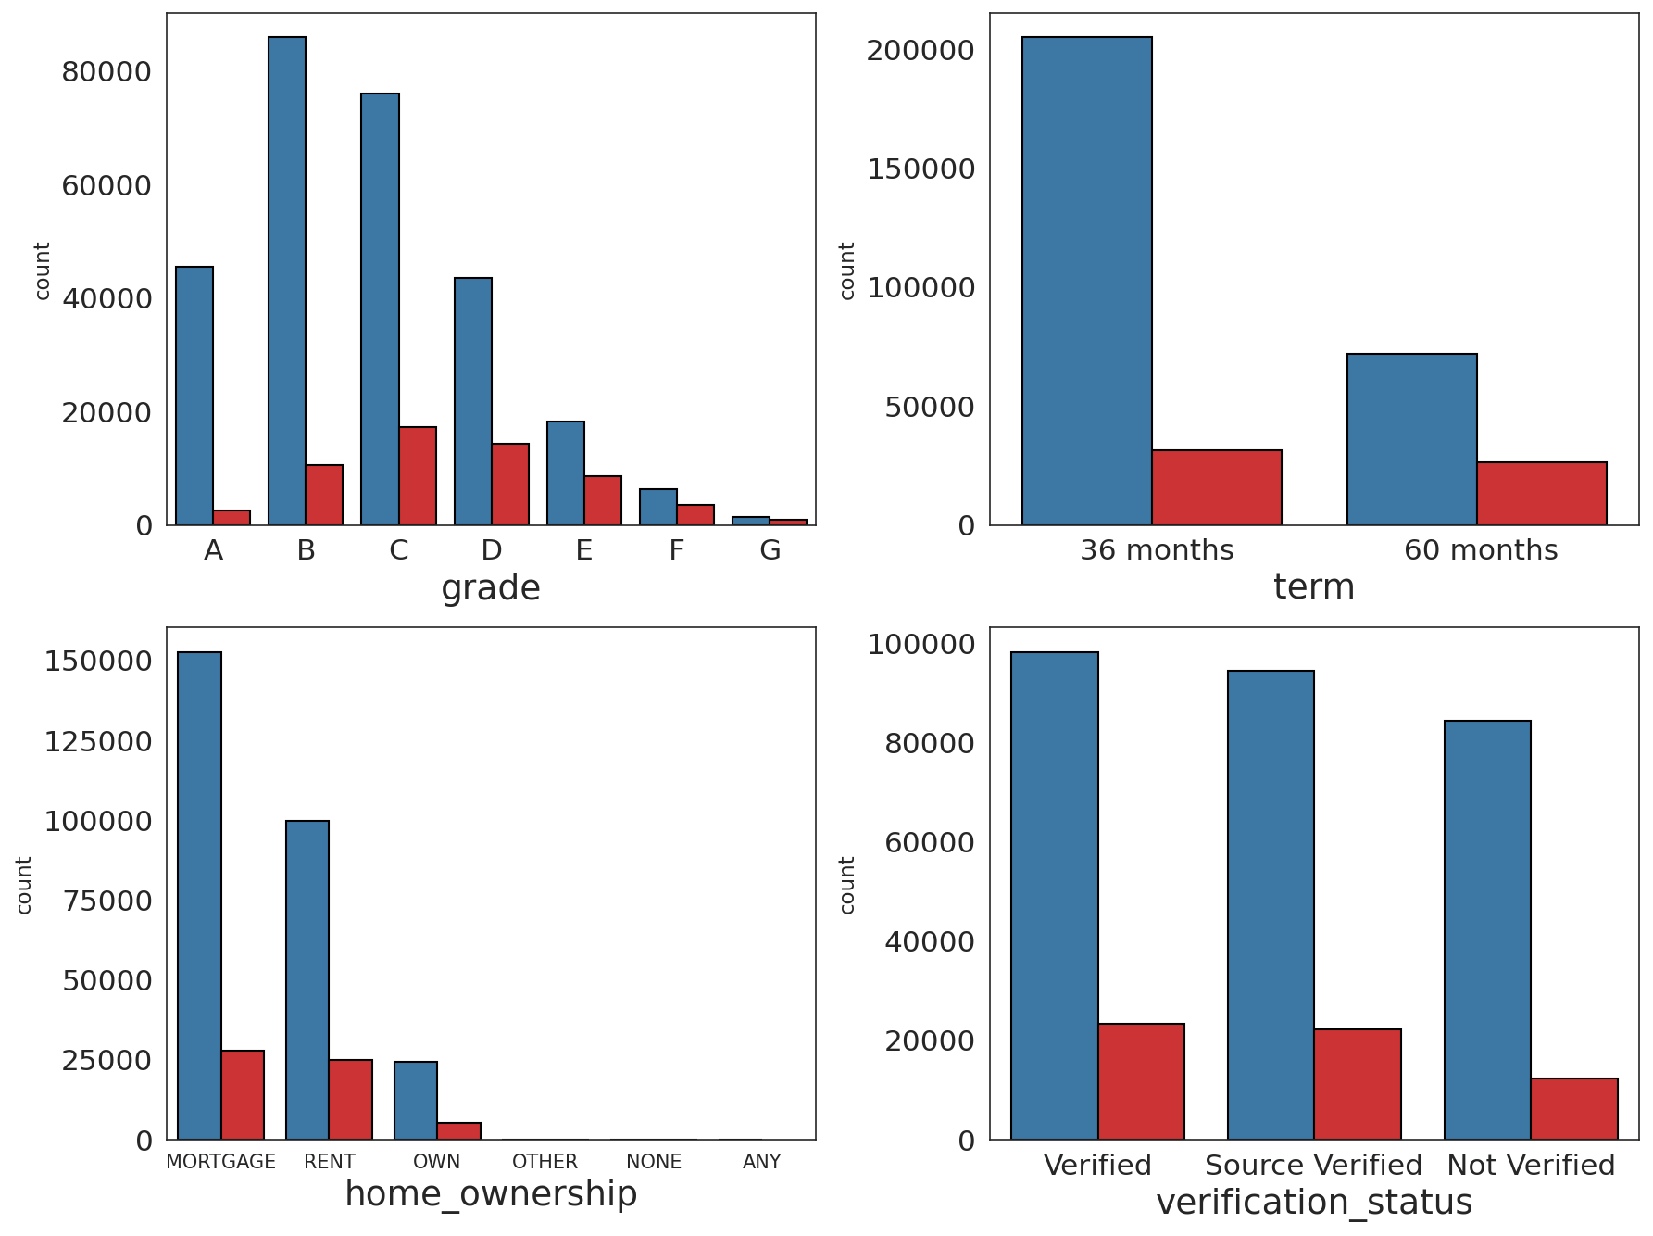
\includegraphics[width=\textwidth,
        height=0.4\textheight,]{image/vlz_lending_club/3_cate_dist_lend.pdf}
    \end{subfigure}
    
    \caption{Phân phối các biến phân loại theo nhãn \texttt{target} --- Lending Club. {\newline \small (Trong đó, màu xanh: \texttt{target}~=~0 và màu đỏ: \texttt{target}~=~1)}}
    \label{fig:cate_dist_lending}
\end{figure}

% =========================================================================
% KHỐI HÌNH: TƯƠNG QUAN
% =========================================================================
\FloatBarrier
\vspace{0.5em}
\noindent
\textbf{Ma trận tương quan} 

Trên Australian (Hình \ref{fig:corr_aus}), hầu hết các cặp biến có tương quan rất thấp, ngoại trừ cặp \texttt{YearsEmployed}-\texttt{Employed} có tương quan dương vừa phải, phản ánh mối liên hệ tự nhiên giữa tình trạng việc làm và thâm niên. Trên German (Hình \ref{fig:corr_ger}), cặp \texttt{month\_duration} và \texttt{credit\_amount} có tương quan dương đáng chú ý - khoản vay lớn hơn thường đi kèm với thời hạn hoàn trả dài hơn, một quan hệ hợp lý về mặt nghiệp vụ tín dụng. Trên Lending Club (Hình \ref{fig:corr_lend}), không gian biến rộng hơn nhiều với 36 biến số, xuất hiện một số cụm tương quan nội bộ giữa các biến cùng nhóm như nhóm biến đếm tài khoản (\texttt{num\_bc\_tl}, \texttt{num\_il\_tl}, \texttt{num\_actv\_rev\_tl}) và nhóm biến thời gian tháng. Đặc biệt, cặp \texttt{fico\_range\_low} và \texttt{int\_rate} có tương quan âm rõ ràng, phản ánh đúng cơ chế định giá rủi ro: điểm tín dụng cao tương ứng với lãi suất thấp hơn. Sự hiện diện của các cụm tương quan này là động lực cho bước L\_Pro sau này.

\vspace{1em}
\begin{figure}[htbp]
    \centering
    \begin{subfigure}[b]{\textwidth}
        \centering
        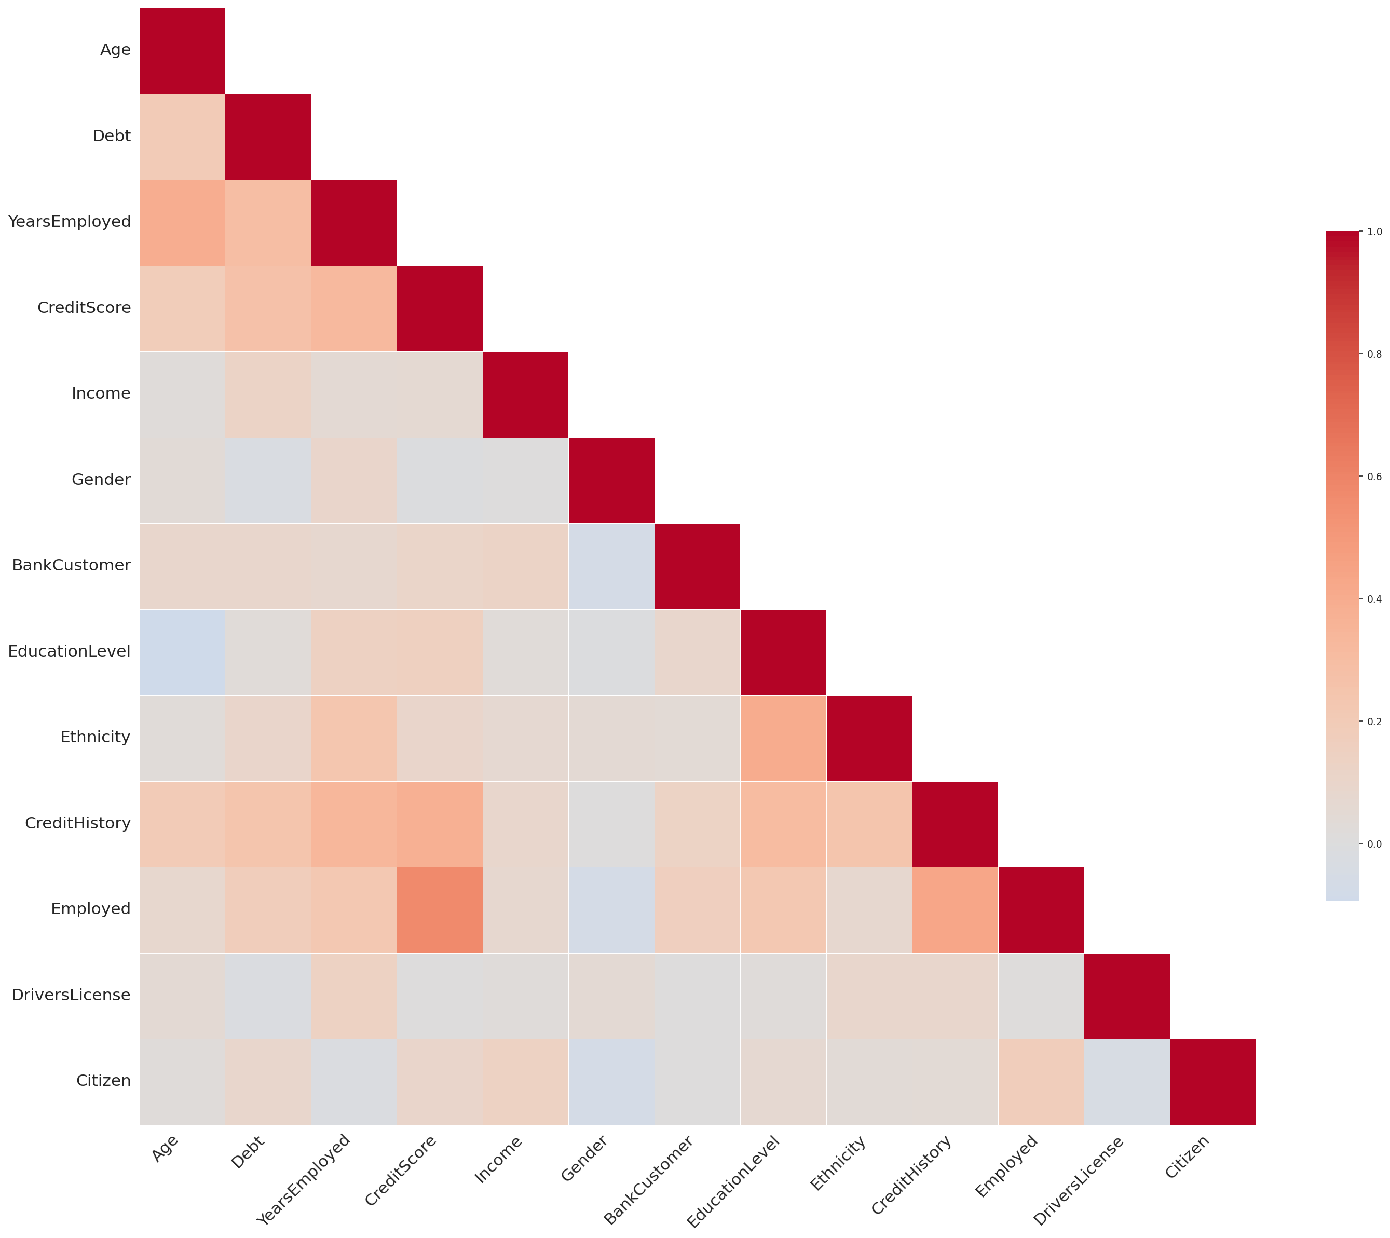
\includegraphics[width=\textwidth]{image/vlz_australian/4_cor_au.pdf}
    \end{subfigure}
    \caption{Ma trận tương quan giữa các biến số liên tục trên Australian Credit}
    \label{fig:corr_aus}
\end{figure}

\begin{figure}[htbp]
    \centering
    \begin{subfigure}[b]{\textwidth}
        \centering
        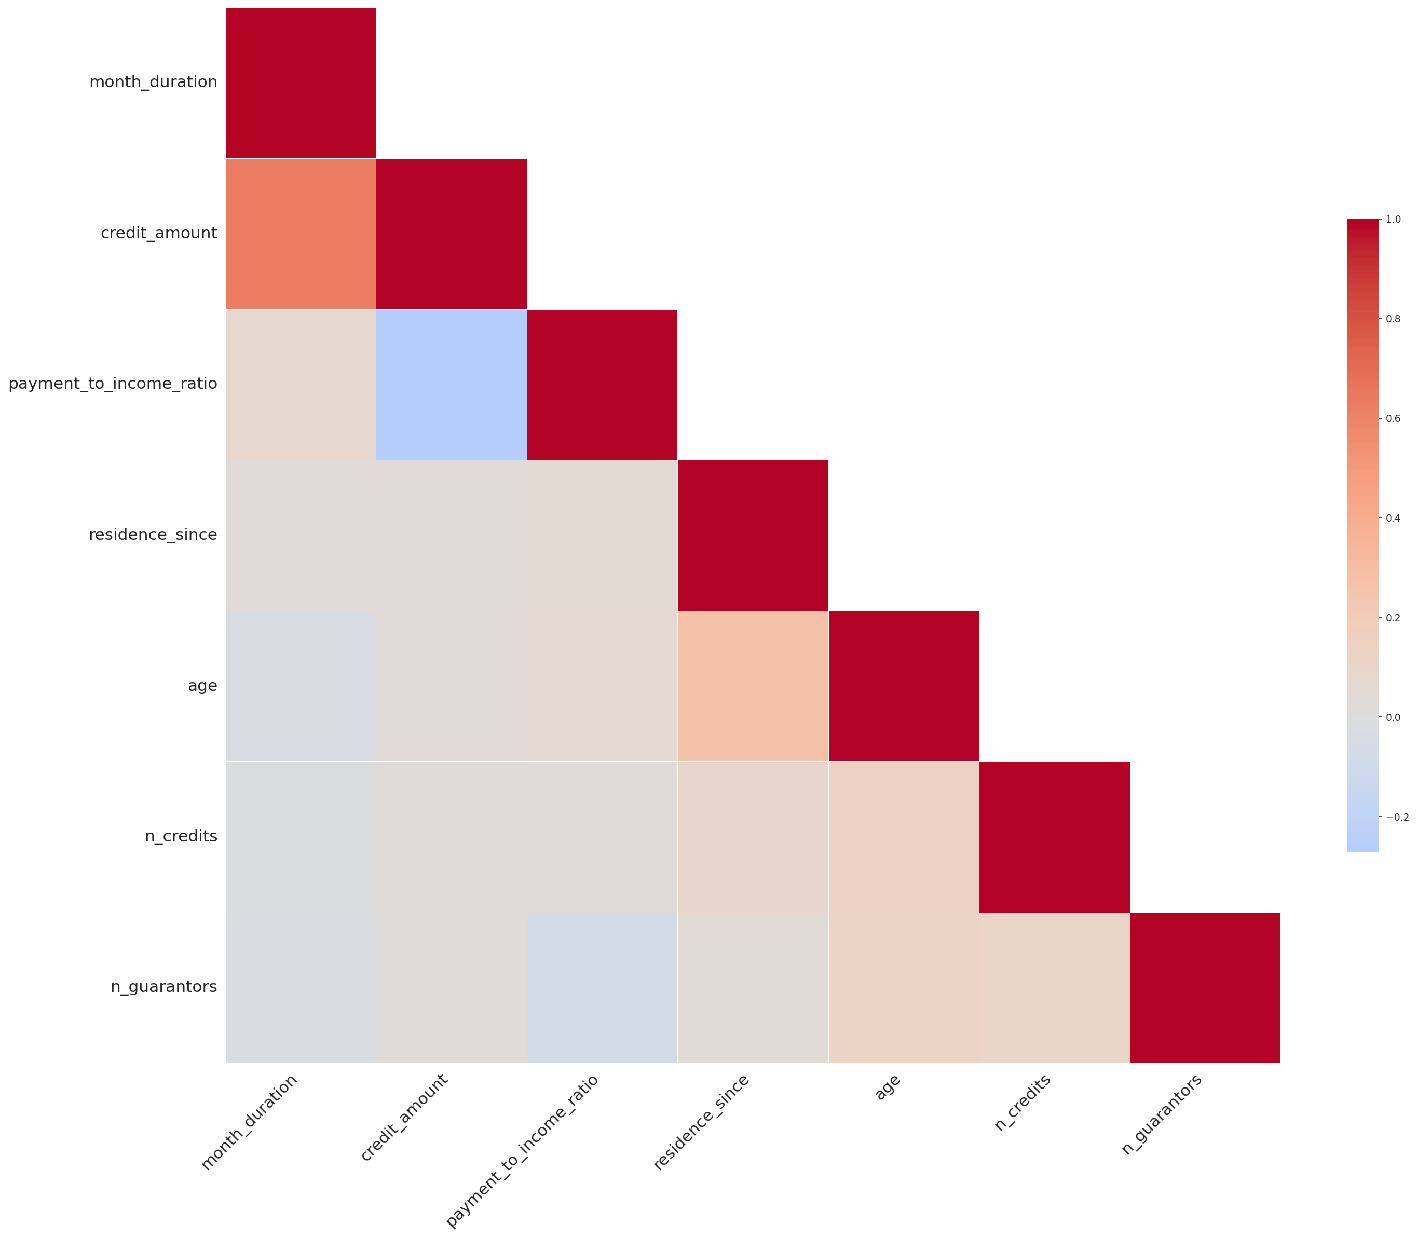
\includegraphics[width=\textwidth]{image/vlz_germany/4_cor_ger.pdf}
    \end{subfigure}
    
    \caption{Ma trận tương quan giữa các biến số liên tục trên German Credit}
    \label{fig:corr_ger}
\end{figure}

\newpage
\begin{figure}[htbp]
    \centering
    \begin{subfigure}[b]{\textwidth}
        \centering
        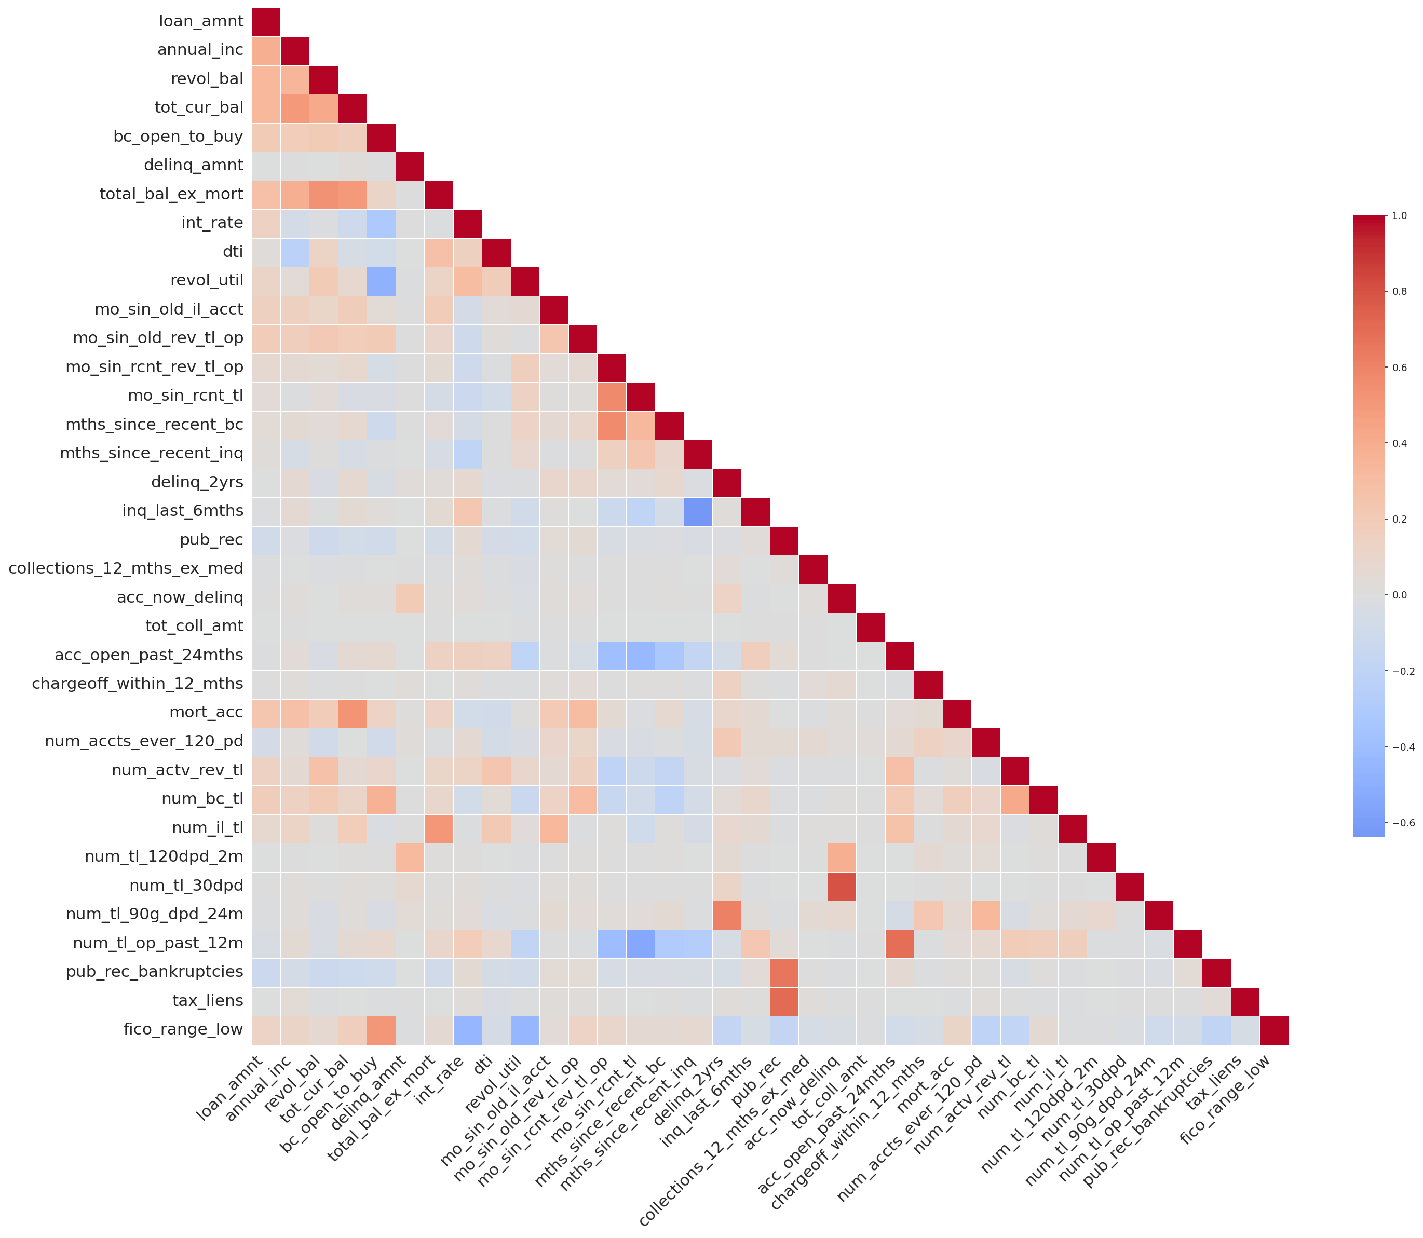
\includegraphics[width=\textwidth]{image/vlz_lending_club/4_cor_lend.pdf}
    \end{subfigure}
    
    \caption{Ma trận tương quan giữa các biến số liên tục trên Lending Club}
    \label{fig:corr_lend}
\end{figure}

\subsection{Xử lý dữ liệu}
\subsubsection{Mã hóa đặc trưng phân loại}
\noindent
Trước khi đưa dữ liệu vào pipelines xử lý dữ liệu, các biến phân loại cần được chuyển hóa thành dạng số để các thuật toán có thể xử lý. Tuy nhiên, không phải mọi biến phân loại đều có thể được mã hóa theo cùng một cách. Nghiên cứu này phân biệt rõ hai nhóm đặc trưng theo bản chất thống kê: biến thứ tự (ordinal) có quan hệ phân cấp nội tại giữa các giá trị, và biến danh nghĩa (nominal) không có thứ bậc tự nhiên giữa các nhóm. Việc áp dụng nhầm phương pháp mã hóa cho từng loại có thể đưa vào mô hình các quan hệ thứ tự giả tạo, dẫn đến sai lệch trong học cấu trúc mạng Bayes.

Đối với bộ dữ liệu Australian, toàn bộ biến phân loại trong tập dữ liệu gốc đã được mã hóa sẵn dưới dạng số nguyên, do đó không cần thực hiện bước mã hóa bổ sung.

Đối với bộ dữ liệu German, năm biến thứ tự được mã hóa thủ công theo ánh xạ phân cấp có ý nghĩa nghiệp vụ. Cụ thể, \texttt{status\_account} được ánh xạ theo mức độ số dư tài khoản từ âm đến dương (0: dưới 0 DM $\rightarrow$ 3: không có tài khoản thanh toán); \texttt{credit\_history} được sắp xếp theo mức độ tin cậy tín dụng tăng dần từ tài khoản có vấn đề đến lịch sử thanh toán hoàn hảo; \texttt{status\_savings} phản ánh quy mô tiết kiệm tăng dần; \texttt{years\_employment} biểu diễn thâm niên làm việc từ thất nghiệp đến trên 7 năm; \texttt{job} thể hiện bậc nghề nghiệp từ lao động phổ thông đến quản lý cấp cao. Tám biến danh nghĩa còn lại gồm \texttt{purpose}, \texttt{status\_and\_sex}, \texttt{secondary\_obligor}, \texttt{collateral}, \texttt{other\_installment\_plans}, \texttt{housing}, \texttt{telephone} và \texttt{is\_foreign\_worker} không có quan hệ thứ bậc tự nhiên giữa các giá trị, do đó được mã hóa tự động bằng \texttt{OrdinalEncoder} với vai trò định danh số nguyên thuần túy. Cách tiếp cận này phù hợp với yêu cầu của mạng Bayes vì mô hình học cấu trúc xác suất từ tần suất quan sát thực tế, không giả định quan hệ tuyến tính giữa các giá trị mã hóa.

Đối với bộ dữ liệu Lending Club, bốn biến thứ tự được ánh xạ thủ công theo logic nghiệp vụ rõ ràng. \texttt{grade} được ánh xạ từ A (0) đến G (6) theo chiều rủi ro tăng dần, phản ánh đúng hệ thống xếp hạng tín dụng nội bộ của Lending Club. \texttt{emp\_length} biểu diễn thâm niên làm việc từ không xác định (0) đến trên 10 năm (11). \texttt{verification\_status} phản ánh mức độ xác minh thu nhập tăng dần từ chưa xác minh đến đã xác minh đầy đủ. \texttt{term} mã hóa kỳ hạn vay với 36 tháng là 0 và 60 tháng là 1. Sáu biến danh nghĩa gồm \texttt{home\_ownership}, \texttt{purpose}, \texttt{addr\_state}, \texttt{initial\_list\_status}, \texttt{debt\_settlement\_flag} và \texttt{hardship\_flag} được mã hóa tự động bằng \texttt{OrdinalEncoder}. Ngoài ra, biến thời gian \texttt{earliest\_cr\_line} lưu dưới dạng chuỗi tháng-năm được chuyển hóa thành biến số liên tục \texttt{mths\_since\_earliest\_cr} - số tháng tính từ thời điểm mở dòng tín dụng đầu tiên đến mốc tham chiếu tháng 1/2015, qua đó bảo toàn thông tin thâm niên tín dụng dưới dạng có thể so sánh định lượng.

\subsubsection{Chia tập huấn luyện và kiểm tra}
\noindent
Để đảm bảo tính khách quan trong đánh giá mô hình, toàn bộ dữ liệu được chia thành các tập con riêng biệt trước khi áp dụng bất kỳ bước tiền xử lý nào liên quan đến máy học. Cả ba bộ dữ liệu đều sử dụng tỷ lệ chia 60/40, trong đó 60\% được dùng làm tập huấn luyện và 40\% còn lại được giữ lại làm tập kiểm tra. Việc chia tập được thực hiện trước các bước SMOTE, Lasso và K-means nhằm tránh hiện tượng rò rỉ dữ liệu (data leakage) — tức là thông tin từ tập kiểm tra vô tình ảnh hưởng đến quá trình huấn luyện mô hình, dẫn đến đánh giá hiệu suất lạc quan giả tạo.

\begin{table}[htbp]
    \centering
    \caption{Phân phối biến mục tiêu sau khi chia tập dữ liệu}
    \label{tab:train_test_split}
    \renewcommand{\arraystretch}{1.3} % Tăng khoảng cách các dòng để bảng thoáng và đẹp hơn
    \begin{tabular}{|l|c|c|c|c|}
        \hline
        \textbf{Bộ dữ liệu} & \textbf{Tập} & \textbf{Không vỡ nợ} & \textbf{Vỡ nợ} & \textbf{Tổng} \\ 
        \hline
        \multirow{3}{*}{Australian} 
        & Train & 197 & 217 & 414 \\ \cline{2-5}
        & Val & 58 & 80 & 138 \\ \cline{2-5}
        & Test  & 52 & 86 & 138 \\ 
        \hline
        \multirow{3}{*}{German} 
        & Train & 418 & 182 & 600 \\ \cline{2-5}
        & Val & 145 & 55 & 200 \\ \cline{2-5}
        & Test  & 137 & 63 & 200 \\ 
        \hline
        \multirow{3}{*}{Lending Club} 
        & Train & 12,579 & 5,421 & 18,000 \\ \cline{2-5}
        & Val & 4,190 & 1,810 & 6,000 \\ \cline{2-5}
        & Test  & 4,231  & 1,769 & 6,000 \\ 
        \hline
    \end{tabular}
\end{table}

Sau khi toàn bộ đường ống tiền xử lý hoàn tất, tập kiểm tra ban đầu (40\%) sẽ được chia tiếp thành hai phần bằng nhau. Phần thứ nhất đóng vai trò tập validation dùng để tinh chỉnh ngưỡng phân loại, trong khi phần thứ hai được giữ nguyên làm tập test thực sự để báo cáo kết quả cuối cùng. Như vậy, tỷ lệ phân chia tổng thể là 60\% huấn luyện, 20\% validation và 20\% kiểm tra.

\subsubsection{Cân bằng dữ liệu (S\_Pro)}
\noindent
Như đã phân tích tại \ref{fig:class_imbalance}, ba bộ dữ liệu thực nghiệm đều biểu hiện mức độ mất cân bằng lớp ở các mức độ khác nhau. Sự chênh lệch này, nếu không được xử lý, sẽ khiến quá trình học cấu trúc mạng Bayes bị lệch về phía lớp đa số, dẫn đến bảng xác suất có điều kiện ước lượng thiên vị và suy giảm khả năng nhận diện rủi ro thực sự. Do đó, bước S\_Pro được áp dụng trên tập huấn luyện ngay sau khi chia tập, trước mọi thao tác tiền xử lý tiếp theo, nhằm đảm bảo không có thông tin từ tập kiểm tra rò rỉ vào quá trình tổng hợp mẫu.

Một điểm kỹ thuật quan trọng là cả ba bộ dữ liệu đều chứa hỗn hợp giữa biến liên tục và biến phân loại. Thuật toán SMOTE tiêu chuẩn \citep{chawla2002smote} vốn được thiết kế cho không gian đặc trưng thuần liên tục, với cơ chế nội suy tuyến tính theo công thức \ref{eq:3.1} khi áp dụng trực tiếp lên biến phân loại sẽ tạo ra các giá trị trung gian vô nghĩa về mặt ngữ nghĩa, chẳng hạn như một trạng thái tài khoản mang giá trị thập phân 2.4 hay một mã mục đích vay bằng 1.73. Để khắc phục hạn chế này, nghiên cứu sử dụng biến thể SMOTE-NC (Synthetic Minority Over-sampling Technique for Nominal and Continuous features). Với mỗi mẫu tổng hợp mới, các biến liên tục vẫn được nội suy theo Công thức \ref{eq:3.1}, trong khi giá trị của từng biến phân loại được quyết định bằng cơ chế bỏ phiếu đa số (majority voting) trên tập $k$ láng giềng gần nhất, tức là chọn giá trị phân loại xuất hiện nhiều nhất trong vùng lân cận của mẫu gốc, qua đó đảm bảo tính hợp lệ về mặt ngữ nghĩa của các quan sát được sinh ra. Mã giả của thuật toán được trình bày như sau:

\vspace{0.5em}
\begin{algorithm}[H]
\caption{Mã giả của thuật toán SMOTE-NC}
\label{alg:smote_nc}

\vspace{0.5em}
\textbf{Input:} Tập mẫu thiểu số $X_{min}$, tập chỉ số biến phân loại $\mathcal{C}$, số láng giềng $k$, tỷ lệ tổng hợp $N$.

\vspace{0.5cm}

\textbf{Output:} Tập mẫu tổng hợp $X_{syn}$.

\begin{tcolorbox}
\begin{algorithmic}[1]
    \State $X_{syn} \gets \emptyset$
    \For{mỗi $x_i \in X_{min}$}
        \State Tính khoảng cách từ $x_i$ đến các mẫu khác trong $X_{min}$, trong đó biến liên tục dùng khoảng cách Euclidean và biến phân loại dùng giá trị $0$ (cùng nhãn) hoặc $\sigma_c$ (khác nhãn, với $\sigma_c$ là độ lệch chuẩn của toàn bộ biến liên tục)
        \State Xác định $k$ láng giềng gần nhất $\mathcal{N}(x_i)$
        \For{$n = 1$ đến $N$}
            \State Chọn ngẫu nhiên $x_{nn}$ từ $\mathcal{N}(x_i)$
            \State Lấy mẫu $\lambda \sim \mathcal{U}(0, 1)$
            \For{mỗi đặc trưng $j$}
                \If{$j \notin \mathcal{C}$} \Comment{Biến liên tục}
                    \State $x_{new}^{(j)} \gets x_i^{(j)} + \lambda \cdot (x_{nn}^{(j)} - x_i^{(j)})$
                \Else \Comment{Biến phân loại}
                    \State $x_{new}^{(j)} \gets \text{mode}\bigl(\{x^{(j)} : x \in \mathcal{N}(x_i)\}\bigr)$
                \EndIf
            \EndFor
            \State $X_{syn} \gets X_{syn} \cup \{x_{new}\}$
        \EndFor
    \EndFor
    \State \textbf{return} $X_{syn}$
\end{algorithmic}
\end{tcolorbox}
\end{algorithm}
\vspace{0.5em}

Trên bộ dữ liệu Australian, 8 biến phân loại được chỉ định tường minh vào tập $\mathcal{C}$, bao gồm \texttt{Gender}, \texttt{BankCustomer}, \texttt{EducationLevel}, \texttt{Ethnicity}, \texttt{CreditHistory}, \texttt{Employed}, \texttt{DriversLicense} và \texttt{Citizen}; 5 biến còn lại (\texttt{Age}, \texttt{Debt}, \texttt{YearsEmployed}, \texttt{CreditScore}, \texttt{Income}) được xử lý theo cơ chế nội suy liên tục. Sau khi áp dụng, tập huấn luyện tăng từ 414 lên 434 quan sát với phân phối lớp đạt cân bằng hoàn toàn ở mức 217 mẫu cho mỗi nhãn. Trên bộ dữ liệu German, 13 biến phân loại được đưa vào $\mathcal{C}$, gồm \texttt{status\_account}, \texttt{credit\_history}, \texttt{status\_savings}, \texttt{years\_employment}, \texttt{job}, \texttt{purpose}, \texttt{status\_and\_sex}, \texttt{secondary\_obligor}, \texttt{collateral}, \texttt{other\_installment\_plans}, \texttt{housing}, \texttt{telephone} và \texttt{is\_foreign\_worker}; 7 biến liên tục còn lại được nội suy trực tiếp. Tập huấn luyện sau S\_Pro tăng từ 600 lên 836 quan sát, đạt phân phối 418 mẫu mỗi lớp. Trên bộ dữ liệu Lending Club, 10 biến phân loại được chỉ định vào $\mathcal{C}$ gồm \texttt{term}, \texttt{grade}, \texttt{emp\_length}, \texttt{verification\_status}, \texttt{home\_ownership}, \texttt{purpose}, \texttt{addr\_state}, \texttt{initial\_list\_status}, \texttt{hardship\_flag} và \texttt{debt\_settlement\_flag}; 36 biến liên tục còn lại được nội suy. Sau S\_Pro, tập huấn luyện tăng từ 18,000 lên 25,158 quan sát với phân phối cân bằng 12,579 mẫu cho mỗi lớp.

Cần nhấn mạnh rằng toàn bộ quy trình tổng hợp mẫu chỉ được thực hiện trên tập huấn luyện. Tập kiểm tra được giữ nguyên phân phối tự nhiên trong suốt tiến trình, nhằm đảm bảo các chỉ số hiệu suất được báo cáo sau này phản ánh trung thực năng lực tổng quát hóa của mô hình trên điều kiện thực tế. Kết quả sau khi áp dụng SMOTE-NC được tổng hợp trong Bảng \ref{tab:smote_results}.

\begin{table}[H]
    \centering
    \caption{Kết quả cân bằng dữ liệu bằng SMOTE-NC trên tập huấn luyện}
    \label{tab:smote_results}
    \renewcommand{\arraystretch}{1.3} % Tăng khoảng cách dòng để bảng thoáng hơn
    \begin{tabular}{|l|c|c|c|}
        \hline
        \textbf{Bộ dữ liệu} & \textbf{Không vỡ nợ} & \textbf{Vỡ nợ} & \textbf{Tổng} \\ \hline
        Australian & 217 & 217 & 434 \\ \hline
        German & 418 & 418 & 836 \\ \hline
        Lending Club & 12,579 & 12,579 & 25,158 \\ \hline
    \end{tabular}
\end{table}

\subsubsection{Chọn lọc đặc trưng (L\_Pro)}
\noindent
Không gian đặc trưng đầu vào sau S\_Pro vẫn còn tương đối lớn, đặc biệt với Lending Club lên đến 46 biến, tiềm ẩn dư thừa thông tin và đa cộng tuyến gây bất lợi cho quá trình học cấu trúc mạng Bayes. Bước L\_Pro do đó được thực hiện nhằm thu gọn không gian biến số xuống mức tối thiểu mà vẫn giữ được năng lực phân biệt rủi ro tín dụng.

Vì biến mục tiêu của bài toán là nhị phân (vỡ nợ/không vỡ nợ) và phần lớn đặc trưng sau bước mã hóa \texttt{OneHotEncoder} mang bản chất biến giả (\textit{dummy}), nghiên cứu sử dụng hồi quy Logistic với hình phạt $L_1$ (Logistic-Lasso) thay vì Lasso hồi quy tuyến tính kinh điển, nhằm phù hợp trực tiếp với cấu trúc xác suất của bài toán phân loại. Tham số cần tối ưu trong mô hình này là hằng số điều chuẩn $C$ nghịch đảo của cường độ phạt $\lambda$, quyết định mức độ thưa của tập đặc trưng được giữ lại.

Ba tiêu chí song song được sử dụng để xác định $C^*$ tối ưu. Tiêu chí thứ nhất là AUC trung bình qua xác nhận chéo 5-fold ($\text{AUC}_{\text{CV}}$), đo trực tiếp khả năng phân biệt của mô hình tại từng giá trị $C$ trong lưới 40 điểm trải đều trên thang $\log_{10}$ từ $10^{-3}$ đến $10^1$. Tiêu chí thứ hai là $\text{AUC}_{\text{BIC}}$, phạt thêm $\text{AUC}_{\text{CV}}$ theo số lượng đặc trưng được chọn:
\begin{equation}
    \text{AUC}_{\text{BIC}}(C) = \text{AUC}_{\text{CV}}(C) - \frac{|\mathcal{S}(C)|}{2n}\ln(n)
    \label{eq:auc_bic_new}
\end{equation}
trong đó $|\mathcal{S}(C)|$ là số đặc trưng có hệ số khác $0$ tại mức $C$ và $n$ là kích thước tập huấn luyện; số hạng phạt đóng vai trò tương tự tiêu chuẩn BIC, khuyến khích mô hình thưa nhất có thể mà vẫn giữ AUC chấp nhận được. Tiêu chí thứ ba là điểm khuỷu (\textit{elbow}) trên đường cong số lượng đặc trưng theo $C$, xác định bằng thuật toán Kneedle - phát hiện vị trí mà việc tăng thêm $C$ không còn mang lại sự gia tăng đáng kể về số đặc trưng được chọn. Giá trị $C^*$ cuối cùng là trung bình hình học của ba ứng viên:
\begin{equation}
    C^* = \exp\left(\frac{\ln C_{\text{AUC}} + \ln C_{\text{BIC}} + \ln C_{\text{elbow}}}{3}\right)
    \label{eq:c_star_new}
\end{equation}

Bên cạnh ba tiêu chí trên, Stability Selection với 100 lần bootstrap và ngưỡng ổn định $0.6$ \citep{meinshausen2010} được thực hiện song song nhằm cung cấp thêm thông tin chẩn đoán về độ tin cậy của từng đặc trưng qua các tập con dữ liệu khác nhau. Toàn bộ bốn thành phần này được trực quan hóa trên cùng một lưới giá trị $C$ như trình bày tại Hình \ref{fig:lpro_au}, \ref{fig:lpro_ger} và \ref{fig:lpro_lend}, cho phép quan sát trực tiếp vị trí hội tụ của các tiêu chí trước khi tổng hợp thành $C^*$.

\vspace{1em}
\begin{figure}[H]
    \centering
    \begin{subfigure}[b]{\textwidth}
        \centering
        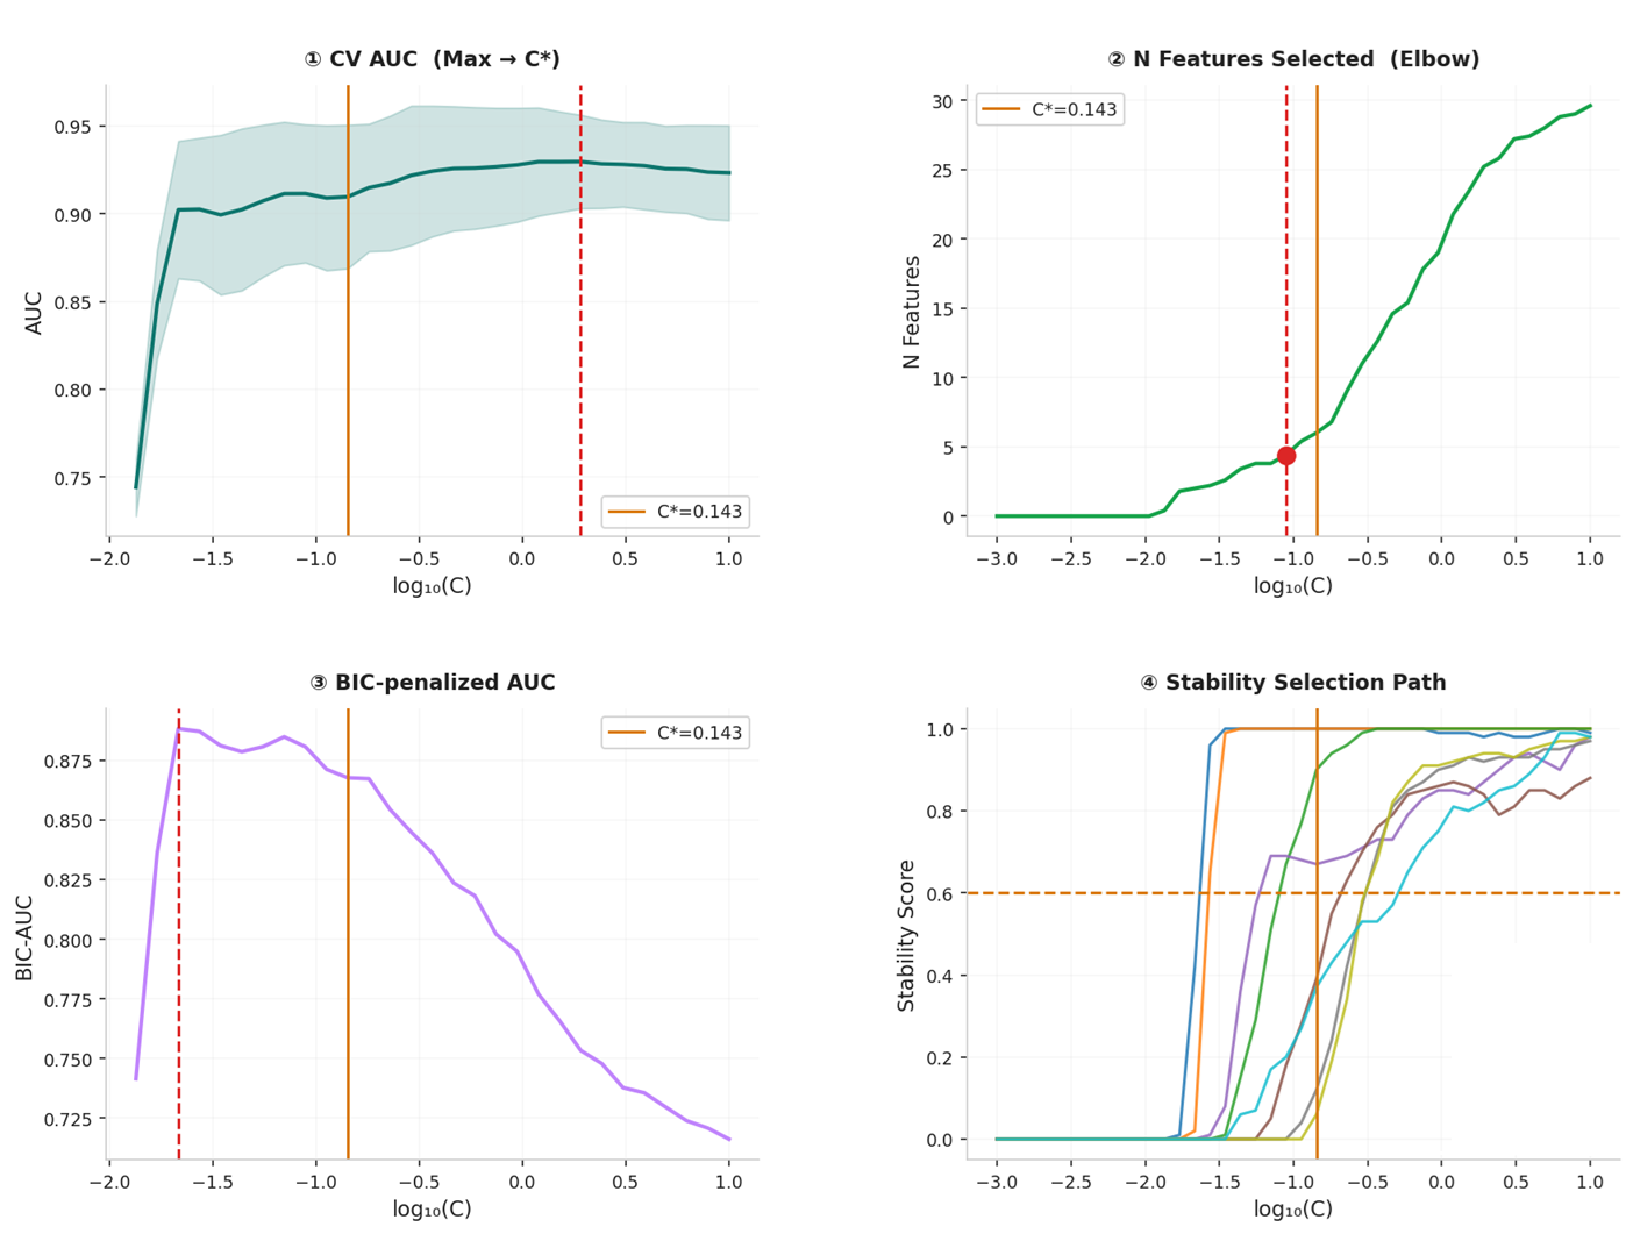
\includegraphics[width=\textwidth]{image/lpro_australian/2_lpro_australian.pdf}
    \end{subfigure}
    
    \caption{Quá trình tối ưu hóa tham số điều chuẩn C trên lưới các tiêu chí trên Australian Credit {
    \newline \small (Trong đó, màu xanh dương = \texttt{CreditScore}, màu cam = \texttt{CreditHistory\_1}, màu xanh lá = \texttt{Income}, tím = \texttt{YearsEmployed}, màu nâu = \texttt{Citizen\_2}, màu xám = \texttt{Age}, màu xanh mạ = \texttt{Employed\_1}, màu xanh trời = \texttt{Debt}; đường ngang đứt nét là ngưỡng \texttt{Threshold = 0.6}})}
    \label{fig:lpro_au}
\end{figure}

\begin{figure}[htbp]
    \centering
    \begin{subfigure}[b]{\textwidth}
        \centering
        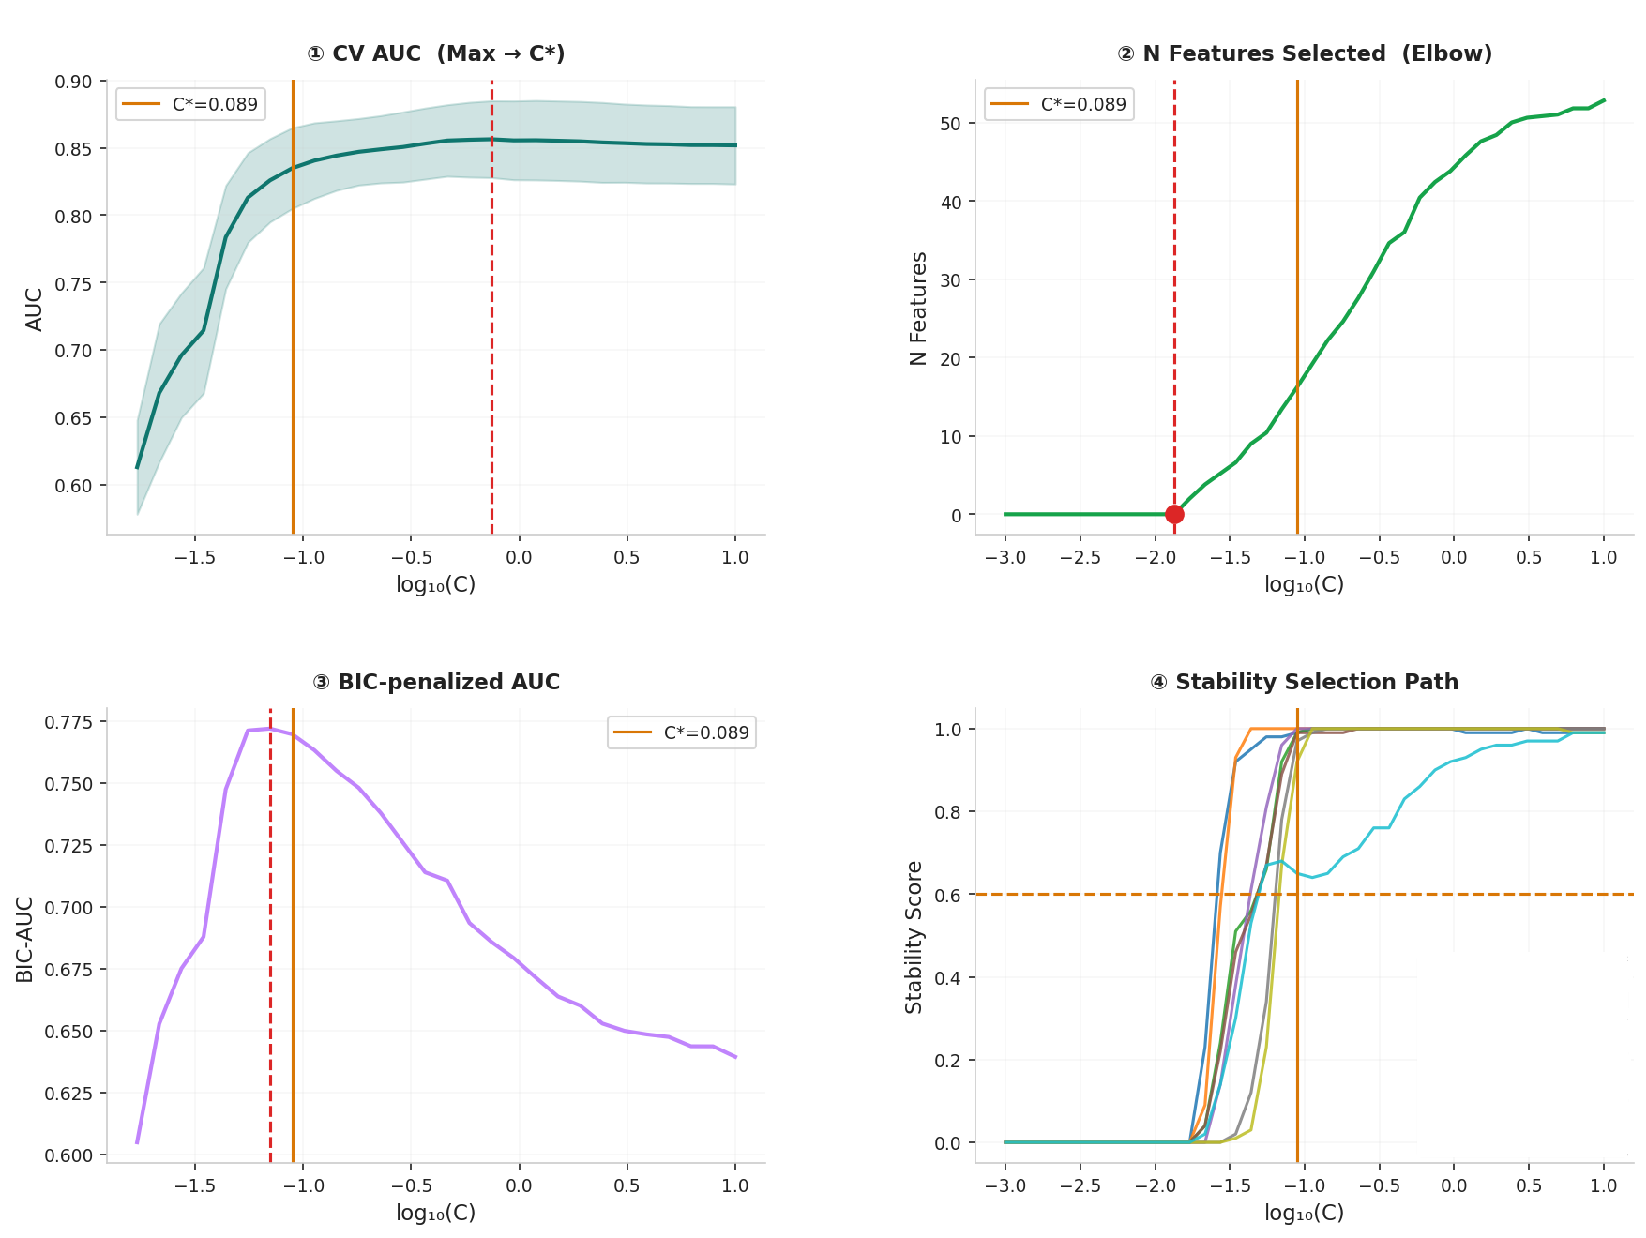
\includegraphics[width=\textwidth]{image/lpro_germany/2_lpro_germany.pdf}
    \end{subfigure}
    
    \caption{Quá trình tối ưu hóa tham số điều chuẩn C trên lưới các tiêu chí trên German Credit {
    \newline \small (Trong đó, màu xanh dương = \texttt{month\_duration}, màu cam = \texttt{age}, màu xanh lá = \texttt{secondary\_obligor\_2.0}, màu tím = \texttt{housing\_1.0}, màu nâu = \texttt{other\_installment\_plans\_1.0}, màu xám = \texttt{status\_account\_3}, màu xanh mạ = \texttt{purpose\_7.0}, màu xanh trời = \texttt{credit\_amount}; đường ngang đứt nét là ngưỡng \texttt{Threshold = 0.6})}}
    \label{fig:lpro_ger}
\end{figure}

\begin{figure}[H]
    \centering
    \begin{subfigure}[b]{\textwidth}
        \centering
        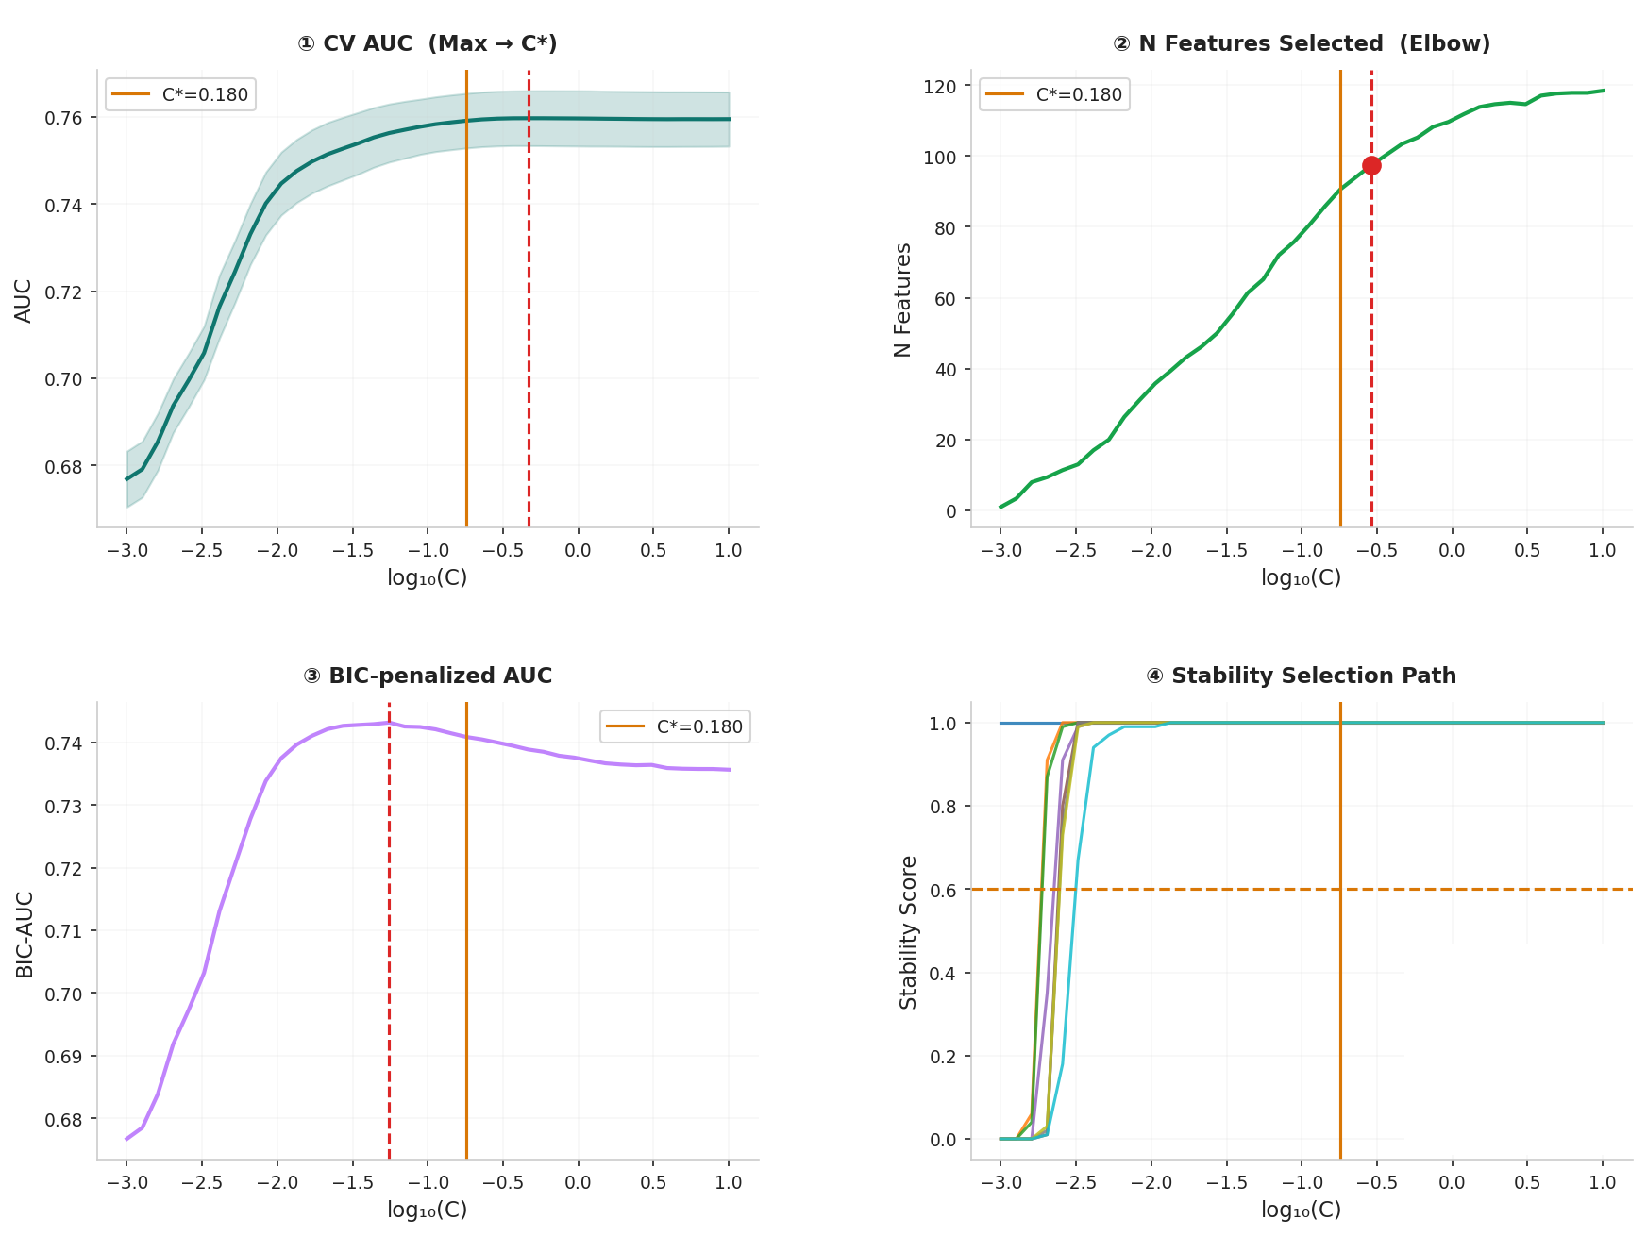
\includegraphics[width=\textwidth]{image/lpro_lending/2_lpro_lending.pdf}
    \end{subfigure}
    
    \caption{Quá trình tối ưu hóa tham số điều chuẩn C trên lưới các tiêu chí trên Lending Club {
    \newline \small (Trong đó, màu xanh dương = \texttt{int\_rate}, màu cam = \texttt{acc\_open\_past\_24mths}, màu xanh lá = \texttt{dti}, tím = \texttt{fico\_range\_low}, màu nâu = \texttt{pub\_rec\_bankruptcies}, màu xám = \texttt{purpose\_2.0}, màu xanh mạ = \texttt{deling\_2yrs}, màu xanh trời = \texttt{mths\_since\_recent\_bc}; đường ngang đứt nét là ngưỡng \texttt{Threshold = 0.6})}}
    \label{fig:lpro_lend}
\end{figure}

\vspace{1em}
Kết quả ba giá trị $C$ ứng viên và $C^*$ tổng hợp trên ba bộ dữ liệu được trình bày tại Bảng \ref{tab:c_selection_criteria}.

\begin{table}[htbp]
    \centering
    \caption{Giá trị tham số $C$ theo từng tiêu chí và $C^*$ tổng hợp}
    \label{tab:c_selection_criteria}
    \renewcommand{\arraystretch}{1.3}
    \begin{tabular}{lcccc}
        \toprule
        \textbf{Bộ dữ liệu} & \textbf{$C_{\text{AUC}}$} & \textbf{$C_{\text{BIC}}$} & \textbf{$C_{\text{elbow}}$} & \textbf{$C^*$} \\ 
        \midrule
        Australian & 1.9145 & 0.0215 & 0.0889 & 0.1425 \\
        German & 0.7444 & 0.0702 & 0.0134 & 0.0889 \\
        Lending Club & 0.4642 & 0.0554 & 0.2894 & 0.1805 \\ 
        \bottomrule
    \end{tabular}
\end{table}

\vspace{1em}
Có thể thấy $C_{\text{AUC}}$ luôn lớn hơn đáng kể so với $C_{\text{BIC}}$ trên cả ba bộ dữ liệu, phản ánh việc tối đa hóa thuần túy AUC có xu hướng giữ lại mô hình kém thưa hơn so với khi có số hạng phạt độ phức tạp. Riêng tại Lending Club, $C_{\text{elbow}}$ lại lớn hơn cả $C_{\text{AUC}}$, cho thấy đường cong số lượng đặc trưng tại bộ dữ liệu này giảm chậm và điểm khuỷu xuất hiện muộn hơn so với hai bộ dữ liệu còn lại, phù hợp với đặc thù không gian đầu vào lớn của Lending Club. Việc lấy trung bình hình học giúp $C^*$ không bị chi phối hoàn toàn bởi tiêu chí cực đoan nhất trong ba ứng viên.

Sau khi xác định $C^*$, một bộ lọc thứ cấp dựa trên Information Value (IV) được áp dụng nhằm loại bỏ các biến có sức phân biệt thực tế quá yếu dù đã được Lasso giữ lại:

\vspace{1em}
\begin{equation}
    \text{IV} = \sum_{i} \left(\text{Dist}_{\text{Event},i} - \text{Dist}_{\text{Non-event},i}\right) \times \ln\left(\frac{\text{Dist}_{\text{Event},i}}{\text{Dist}_{\text{Non-event},i}}\right)
    \label{eq:iv_formula}
\end{equation}

\vspace{1em}
\noindent
với $i$ là chỉ số phân nhóm (\textit{bin}) của biến đặc trưng sau rời rạc hóa. Toàn bộ quy trình ba giai đoạn: xác định $C^*$, trích xuất đặc trưng Lasso, lọc thứ cấp bằng IV được tóm tắt tại Thuật toán \ref{alg:l_pro}.

Trên bộ dữ liệu Australian, Lasso tại $C^* = 0.1425$ chọn được 9 đặc trưng gốc. Sau bộ lọc IV với ngưỡng 0.04, biến \texttt{Gender} bị loại do IV chỉ đạt 0.0001, tập đặc trưng cuối cùng còn 8 biến. Trên bộ dữ liệu German, Lasso tại $C^* = 0.0889$ giữ lại 15 đặc trưng; toàn bộ đều vượt ngưỡng IV 0.05, dẫn đầu là \texttt{secondary\_obligor} ($\text{IV} = 0.6419$), \texttt{other\_installment\_plans} ($\text{IV} = 0.6278$) và \texttt{purpose} ($\text{IV} = 0.6040$), nên không biến nào bị loại. Trên bộ dữ liệu Lending Club, Lasso tại $C^* = 0.1805$ chọn 45 trong 46 biến; bộ lọc IV với ngưỡng 0.03 loại tiếp 18 biến, giữ lại 27 đặc trưng, trong đó \texttt{num\_tl\_op\_past\_12m} ($\text{IV} = 1.1613$), \texttt{inq\_last\_6mths} ($\text{IV} = 0.9930$) và \texttt{num\_actv\_rev\_tl} ($\text{IV} = 0.7156$) là ba biến có sức phân biệt mạnh nhất, phản ánh hành vi tín dụng gần đây và mức độ hoạt động tài khoản là tín hiệu rủi ro chủ đạo của bộ dữ liệu này.

\vspace{1em}
Kết quả sau khi chọn lọc đặc trưng được tổng hợp trong Bảng \ref{tab:lasso_results}.

\begin{table}[htbp]
    \centering
    \caption{Kết quả chọn lọc đặc trưng sau Lasso}
    \label{tab:lasso_results}
    \renewcommand{\arraystretch}{1.3} % Tăng khoảng cách dòng để bảng thoáng hơn
    \begin{tabular}{|l|c|c|c|c|}
        \hline
        \textbf{Bộ dữ liệu} & \textbf{$C^*$} & \textbf{Lasso chọn} & \textbf{Ngưỡng IV} & \textbf{Sau bộ lọc IV} \\ \hline
        Australian & 0.1425 & 9 & 0.04 & 8 \\ \hline
        German & 0.0889 & 15 & 0.05 & 15 \\ \hline
        Lending Club & 0.1805 & 45 & 0.03 & 27 \\ \hline
    \end{tabular}
\end{table}


\vspace{0.5em}
\begin{algorithm}[H]
\caption{Mã giả của quy trình chọn lọc đặc trưng L\_Pro}
\label{alg:l_pro}

\vspace{0.5em}
\textbf{Input:} Tập huấn luyện $(X_{\text{train}}, y_{\text{train}})$ sau S\_Pro; lưới tham số $\mathcal{C} = \{C_1, C_2, \dots, C_{40}\}$ trải đều trên thang $\log_{10}$ từ $10^{-3}$ đến $10^1$; số fold $K = 5$; số bootstrap $B = 100$; ngưỡng ổn định $\tau = 0.6$; ngưỡng IV $\delta$.

\vspace{0.5cm}

\textbf{Output:} Tập đặc trưng cuối cùng $\mathcal{F}^*$ đưa vào K\_Pro.

\begin{tcolorbox}
\begin{algorithmic}[1]
    \Statex \textbf{\textit{// Giai đoạn 1: Xác định $C^*$ tối ưu}}
    \For{mỗi $C \in \mathcal{C}$}
        \State Huấn luyện Logistic-Lasso với penalty $L_1$ và tham số $C$ qua $K$-fold cross-validation
        \State $\text{AUC}_{\text{CV}}(C) \gets$ AUC trung bình trên $K$ fold
        \State $|\mathcal{S}(C)| \gets$ số đặc trưng có $|\hat{\beta}_j| > 0$ trung bình trên $K$ fold
        \State $\text{AUC}_{\text{BIC}}(C) \gets \text{AUC}_{\text{CV}}(C) - \frac{|\mathcal{S}(C)|}{2n}\ln(n)$
        
        \For{$b = 1$ đến $B$} \Comment{Stability Selection}
            \State Lấy mẫu con ngẫu nhiên $50\%$ từ $(X_{\text{train}}, y_{\text{train}})$
            \State Huấn luyện Lasso tại $C$; ghi nhận tập đặc trưng được chọn $\mathcal{S}^{(b)}(C)$
        \EndFor
        
        \State $\Pi_j(C) \gets \frac{1}{B}\sum_{b=1}^{B} \mathbf{1}[j \in \mathcal{S}^{(b)}(C)]$ với mỗi đặc trưng $j$ \Comment{Tần suất chọn}
    \EndFor
    
    \State $C_{\text{AUC}} \gets \arg\max_{C} \text{AUC}_{\text{CV}}(C)$
    \State $C_{\text{BIC}} \gets \arg\max_{C} \text{AUC}_{\text{BIC}}(C)$
    \State $C_{\text{elbow}} \gets$ điểm khuỷu trên đường cong $|\mathcal{S}(C)|$ theo thuật toán Kneedle
    \State $C^* \gets \exp\left(\frac{\ln C_{\text{AUC}} + \ln C_{\text{BIC}} + \ln C_{\text{elbow}}}{3}\right)$, làm tròn về giá trị gần nhất trong $\mathcal{C}$

    \vspace{0.3cm}
    \Statex \textbf{\textit{// Giai đoạn 2: Trích xuất đặc trưng tại $C^*$}}
    \State Huấn luyện Lasso trên toàn bộ $X_{\text{train}}$ tại $C^*$
    \State $\mathcal{S}^* \gets \{j : |\hat{\beta}_j| > 0\}$ \Comment{Tập đặc trưng Lasso sơ bộ}

    \vspace{0.3cm}
    \Statex \textbf{\textit{// Giai đoạn 3: Lọc thứ cấp bằng Information Value}}
    \For{mỗi đặc trưng $j \in \mathcal{S}^*$}
        \State Rời rạc hóa $X_j$ thành các bin; tính $\text{IV}_j = \sum_{i} \left(\text{Dist}_{\text{event},i} - \text{Dist}_{\text{non-event},i}\right) \ln\left(\frac{\text{Dist}_{\text{event},i}}{\text{Dist}_{\text{non-event},i}}\right)$
    \EndFor
    
    \State $\mathcal{F}^* \gets \{j \in \mathcal{S}^* : \text{IV}_j \geq \delta\}$
    \State \textbf{return} $\mathcal{F}^*$
\end{algorithmic}
\end{tcolorbox}
\end{algorithm}
\vspace{0.5em}

\newpage
\subsubsection{Rời rạc hóa dữ liệu (K\_Pro)}
\label{sec: 4.2.5}
\noindent
Như đã trình bày tại Mục \ref{sec: 3.1.3}, việc rời rạc hóa các biến liên tục là điều kiện tiên quyết để mạng Bayes có thể tính toán bảng xác suất có điều kiện thông qua thống kê tần suất, bởi lẽ với biến liên tục mang vô hạn giá trị, mỗi tổ hợp cha-con gần như chỉ xuất hiện đúng một lần trong dữ liệu huấn luyện, khiến ước lượng hợp lý cực đại trở nên vô nghĩa do thiếu quan sát lặp lại. Tuy nhiên, áp dụng trực tiếp thuật toán K-means theo Công thức \ref{eq: 3.3} lên các biến tài chính nguyên gốc - vốn có phân phối lệch nặng do đặc tính của dữ liệu tín dụng (thu nhập, dư nợ, số dư tín dụng thường tập trung dày ở mức thấp và kéo đuôi dài về phía giá trị cao) - sẽ dẫn đến hiện tượng các cụm bị chi phối bởi một vài điểm ngoại lai cực đoan, khiến phần lớn quan sát bị dồn vào một hoặc hai bin trong khi các bin còn lại gần như trống.

Để khắc phục hạn chế này, quy trình thực nghiệm bổ sung một bước biến đổi phân phối trước khi đưa dữ liệu vào K-means theo Thuật toán \ref{alg:kmeans_discretization} đã trình bày tại Mục \ref{sec: 3.1.3}. Bước bổ sung này áp dụng phép biến đổi lũy thừa Yeo-Johnson, được định nghĩa theo bốn trường hợp tùy vào dấu của giá trị gốc $x$ và tham số hình dạng $\lambda$:
\begin{equation}
\psi(x; \lambda) =
\begin{cases}
\dfrac{(x+1)^{\lambda} - 1}{\lambda}, & \lambda \neq 0,\ x \geq 0 \\[8pt]
\ln(x+1), & \lambda = 0,\ x \geq 0 \\[8pt]
-\dfrac{(-x+1)^{2-\lambda} - 1}{2-\lambda}, & \lambda \neq 2,\ x < 0 \\[8pt]
-\ln(-x+1), & \lambda = 2,\ x < 0
\end{cases}
\label{eq:yeo_johnson}
\end{equation}
trong đó tham số $\lambda$ được ước lượng bằng phương pháp hợp lý cực đại trên tập huấn luyện, sao cho phân phối của $\psi(x;\lambda)$ tiệm cận gần nhất với phân phối chuẩn \citep{yeo2000}. Hai nhánh đầu xử lý giá trị không âm theo cùng cơ chế với biến đổi Box-Cox cộng thêm hằng số dịch chuyển, trong khi hai nhánh sau mở rộng công thức sang miền giá trị âm bằng phép phản chiếu qua gốc tọa độ, qua đó khắc phục được hạn chế cố hữu của Box-Cox vốn chỉ xác định trên miền dương. Phép biến đổi này được lựa chọn vì khả năng xử lý cả giá trị âm và bằng $0$, vốn xuất hiện phổ biến trong các biến như chênh lệch nợ hoặc số tháng kể từ sự kiện gần nhất, đồng thời san phẳng độ lệch và giảm ảnh hưởng của giá trị ngoại lai mà không làm mất thông tin như các kỹ thuật cắt ngưỡng (capping) truyền thống.

Đối với bộ dữ liệu Lending Club, do thang đo giữa các biến chênh lệch rất lớn - chẳng hạn \texttt{loan\_amnt} tính bằng nghìn đô-la trong khi \texttt{dti} tính theo phần trăm - một bước chuẩn hóa \texttt{StandardScaler} được thực hiện trước Yeo-Johnson nhằm đưa các biến về cùng thang đo, tránh tình trạng biến có phương sai lớn lấn át quá trình ước lượng tham số biến đổi của các biến còn lại. Sau khi dữ liệu được chuẩn hóa phân phối, thuật toán K-means theo Thuật toán \ref{alg:kmeans_discretization} được áp dụng trên không gian đã biến đổi với số bin cố định $k = 4$ cho toàn bộ các biến liên tục. Số bin $k = 4$ được lựa chọn nhằm cân bằng giữa hai mục tiêu đối nghịch: duy trì đủ độ phân giải để các bin phản ánh được sự khác biệt về rủi ro tín dụng giữa các mức giá trị, đồng thời tránh tình trạng phân mảnh quá mức khiến một số tổ hợp trạng thái cha-con trong mạng Bayes rơi vào vùng dữ liệu thưa. Ranh giới của từng bin sau đó được ánh xạ ngược về thang giá trị gốc bằng cách lấy giá trị nhỏ nhất và lớn nhất thực tế của các quan sát rơi vào bin đó trên tập huấn luyện, đảm bảo các khoảng giá trị được báo cáo phản ánh đúng phân phối dữ liệu chứ không phải ranh giới lý thuyết của cụm trong không gian đã biến đổi.

Kết quả rời rạc hóa trên bộ dữ liệu Australian được trình bày tại Bảng \ref{tab:australian_features_kpro}. Biến \texttt{Debt} được chia thành bốn khoảng $[0.00; 1.08)$, $[1.08; 3.29)$, $[3.29; 8.00)$ và $[8.00; 28.00]$, trong đó tỷ lệ vỡ nợ giảm dần từ $54.78\%$ ở bin thấp nhất xuống còn $32.41\%$ ở bin cao nhất - một xu hướng có phần phản trực giác nếu xét theo logic thông thường rằng nợ càng cao thì rủi ro càng lớn, song có thể giải thích bởi việc các khoản nợ lớn thường gắn với hồ sơ tín dụng đã được thẩm định kỹ và có tài sản đảm bảo tương ứng. Biến \texttt{YearsEmployed} thể hiện quan hệ đơn điệu rõ ràng hơn, với tỷ lệ vỡ nợ giảm mạnh từ $72.16\%$ ở nhóm có thời gian làm việc dưới $0.54$ năm xuống còn $19.23\%$ ở nhóm trên $4.33$ năm, phản ánh đúng trực giác rằng thâm niên công việc ổn định tương quan nghịch với rủi ro tín dụng. Biến \texttt{CreditScore} cho thấy mức phân tách event rate mạnh nhất trong số các biến liên tục của bộ dữ liệu này, từ $71.61\%$ tại bin thấp nhất xuống chỉ còn $9.18\%$ tại bin cao nhất, củng cố vai trò của biến này như một chỉ báo rủi ro hàng đầu.

Kết quả rời rạc hóa trên bộ dữ liệu German được trình bày tại Bảng \ref{tab:german_features_kpro}. Trên bộ dữ liệu German, biến \texttt{month\_duration} - thời hạn vay tính theo tháng - biểu hiện quan hệ đồng biến với rủi ro vỡ nợ, tăng từ $14.00\%$ ở nhóm vay ngắn hạn (4-9 tháng) lên $70.79\%$ ở nhóm vay dài hạn (31-60 tháng), phù hợp với lý thuyết tài chính rằng kỳ hạn vay càng dài thì rủi ro tín dụng tích lũy càng lớn do thời gian phơi nhiễm trước các cú sốc thu nhập kéo dài hơn. Biến \texttt{age} cho thấy xu hướng ngược lại, với tỷ lệ vỡ nợ giảm từ $57.38\%$ ở nhóm tuổi 19-25 xuống còn $32.74\%$ ở nhóm trên 43 tuổi, phản ánh sự ổn định tài chính tăng dần theo độ tuổi. Biến \texttt{credit\_amount} không thể hiện quan hệ đơn điệu, dao động trong khoảng $43.65\%$-$62.15\%$ qua các bin, cho thấy quy mô khoản vay đơn thuần không phải là yếu tố quyết định mạnh đến khả năng vỡ nợ trên bộ dữ liệu này nếu tách biệt khỏi các biến khác.

Kết quả rời rạc hóa trên bộ dữ liệu Lending Club được trình bày tại Bảng \ref{tab:lending_club_features_kpro}. Trên bộ dữ liệu Lending Club, biến \texttt{int\_rate} - lãi suất cho vay - thể hiện quan hệ đồng biến rõ rệt và mạnh nhất trong toàn bộ các biến liên tục được khảo sát, với tỷ lệ vỡ nợ tăng từ $22.54\%$ ở bin lãi suất thấp nhất ($6.00\%$-$10.80\%$) lên đến $69.09\%$ ở bin lãi suất cao nhất ($19.59\%$-$26.06\%$), nhất quán với cơ chế định giá rủi ro của các nền tảng cho vay ngang hàng, theo đó lãi suất được ấn định cao hơn cho các khoản vay được đánh giá rủi ro lớn hơn ngay từ khâu thẩm định ban đầu. Biến \texttt{dti} (tỷ lệ nợ trên thu nhập) cũng cho thấy xu hướng đồng biến nhất quán, từ $38.02\%$ lên $56.03\%$ qua bốn bin, phù hợp với kỳ vọng rằng gánh nặng nợ tương đối cao so với thu nhập làm suy giảm khả năng trả nợ. Ngược lại, các biến phản ánh độ sâu lịch sử tín dụng như \texttt{mo\_sin\_rcnt\_tl} (số tháng kể từ tài khoản tín dụng gần nhất được mở) và \texttt{mths\_since\_recent\_bc} lại thể hiện quan hệ nghịch biến ở bin cao nhất, với tỷ lệ vỡ nợ giảm xuống còn $35.88\%$ và $41.51\%$ tương ứng - cho thấy khách hàng không mở tài khoản tín dụng mới trong thời gian dài có xu hướng ổn định tài chính hơn. Đáng chú ý, biến \texttt{revol\_util} tại bộ dữ liệu này xuất hiện một bin chỉ chứa duy nhất một quan sát với tỷ lệ vỡ nợ $100\%$, một hiện tượng điển hình của rời rạc hóa dựa trên K-means khi tồn tại điểm ngoại lai cực đoan tách biệt hẳn khỏi phần còn lại của phân phối dù đã qua phép biến đổi Yeo-Johnson.

Toàn bộ quy trình \textit{power-transform} và \textit{K-means discretization} được \textit{fit} (ước lượng tham số) duy nhất trên tập huấn luyện, sau đó áp dụng \textit{transform} tương ứng lên tập kiểm tra nhằm tránh rò rỉ thông tin từ tập kiểm tra vào quá trình xác định ranh giới bin.

% ===== BẢNG 4.5: Australian (longtable) =====
\renewcommand{\arraystretch}{1.4}
\begin{longtable}{V{2.9cm}D{9.3cm}S{2.4cm}}
    \caption{Mô tả các đặc trưng đã chọn của bộ dữ liệu Australian sau K\_Pro}
    \label{tab:australian_features_kpro} \\
 
    \toprule
    \textbf{Tên biến} & \textbf{Mô tả} & \textbf{States} \\
    \midrule
    \endfirsthead
 
    \multicolumn{3}{c}%
    {{\bfseries \tablename\ \thetable{} (tiếp theo)}} \\
    \toprule
    \textbf{Tên biến} & \textbf{Mô tả} & \textbf{States} \\
    \midrule
    \endhead
 
    \midrule
    \multicolumn{3}{r}{{Tiếp tục ở trang sau...}} \\
    \endfoot
 
    \bottomrule
    \endlastfoot
 
    \varname{CreditHistory} & Lịch sử tín dụng trước đó của người nộp đơn \newline Không, có & 0, 1 \\
    \varname{CreditScore} & Điểm tín dụng của người nộp đơn \newline $(0; 1]$, $(1; 2]$, $(2; 4]$, $(4; 40]$ & 0, 1, 2, 3 \\
    \varname{Employed} & Tình trạng đang đi làm tại thời điểm nộp đơn \newline Không, có & 0, 1 \\
    \varname{YearsEmployed} & Số năm làm việc tại nơi công tác hiện tại \newline $(0.00; 0.54]$, $(0.54; 1.96]$, $(1.96; 4.33]$, $(4.33; 28.50]$ & 0, 1, 2, 3 \\
    \varname{Income} & Thu nhập của người nộp đơn \newline $(1; 5]$, $(5; 51]$, $(51; 679]$, $(679; 51101]$ & 0, 1, 2, 3 \\
    \varname{Debt} & Tổng dư nợ hiện tại của người nộp đơn \newline $(0.00; 1.08]$, $(1.08; 3.29]$, $(3.29; 8.00]$, $(8.00; 28.00]$ & 0, 1, 2, 3 \\
    \varname{Age} & Tuổi của người nộp đơn \newline $(13.75; 21.67]$, $(21.67; 29.17]$, $(29.17; 41.00]$, $(41.00; 80.25]$ & 0, 1, 2, 3 \\
    \varname{Citizen} & Tình trạng quốc tịch/cư trú của người nộp đơn & 1, 2, 3 \\
    \varname{target} & Trạng thái phê duyệt hồ sơ tín dụng \newline Vỡ nợ, không vỡ nợ & 0, 1 \\
 
\end{longtable}
 
% ===== BẢNG 4.6: German Credit (longtable) =====
\renewcommand{\arraystretch}{1.4}
\begin{longtable}{V{2.9cm}D{9.3cm}S{2.4cm}}
    \caption{Mô tả các đặc trưng đã chọn của bộ dữ liệu German Credit sau K\_Pro}
    \label{tab:german_features_kpro} \\
 
    \toprule
    \textbf{Tên biến} & \textbf{Mô tả} & \textbf{States} \\
    \midrule
    \endfirsthead
 
    \multicolumn{3}{c}%
    {{\bfseries \tablename\ \thetable{} (tiếp theo)}} \\
    \toprule
    \textbf{Tên biến} & \textbf{Mô tả} & \textbf{States} \\
    \midrule
    \endhead
 
    \midrule
    \multicolumn{3}{r}{{Tiếp tục ở trang sau...}} \\
    \endfoot
 
    \bottomrule
    \endlastfoot
 
    \varname{status_account} & Tình trạng tài khoản vãng lai của khách hàng tại ngân hàng \newline $< 0$ DM, $0 \leq \dots < 200$ DM, $\geq 200$ DM, no checking account & 0, 1, 2, 3 \\
    \varname{month_duration} & Thời hạn vay tính theo tháng \newline $(4; 9]$, $(9; 17]$, $(17; 31]$, $(31; 60]$ & 0, 1, 2, 3 \\
    \varname{credit_history} & Lịch sử tín dụng của khách hàng \newline No credits taken/all credits paid back duly, all credits at this bank paid back duly, existing credits paid back duly till now, delay in paying off in the past, critical account/other credits existing & 0, 1, 2, 3, 4 \\
    \varname{purpose} & Mục đích vay \newline Car (new), car (used), furniture/equipment, radio/television, domestic appliances, repairs, education, retraining, business, others & 0, 1, 2, 3, 4, 5, 6, 7, 8, 9 \\
    \varname{credit_amount} & Số tiền vay \newline $(250; 1068]$, $(1068; 2279]$, $(2279; 5433]$, $(5433; 18424]$ & 0, 1, 2, 3 \\
    \varname{status_and_sex} & Tình trạng hôn nhân và giới tính \newline Male: divorced/separated, female: divorced/separated/married, male: single, male: married/widowed & 0, 1, 2, 3 \\
    \varname{secondary_obligor} & Người bảo lãnh hoặc đồng vay \newline None, co-applicant, guarantor & 0, 1, 2 \\
    \varname{residence_since} & Số năm cư trú tại nơi ở hiện tại & 1, 2, 3, 4 \\
    \varname{collateral} & Tài sản đảm bảo \newline Real estate, building society savings agreement/life insurance, car or other, unknown/no property & 0, 1, 2, 3 \\
    \varname{age} & Tuổi của khách hàng \newline $(19; 25]$, $(25; 32]$, $(32; 43]$, $(43; 75]$ & 0, 1, 2, 3 \\
    \varname{other_installment_plans} & Các khoản trả góp khác đang có \newline Bank, stores, none & 0, 1, 2 \\
    \varname{housing} & Tình trạng nhà ở \newline Rent, own, for free & 0, 1, 2 \\
    \varname{n_credits} & Số khoản tín dụng hiện có tại ngân hàng này & 1, 2, 3, 4 \\
    \varname{job} & Tình trạng nghề nghiệp \newline Unemployed/unskilled non-resident, unskilled resident, skilled employee/official, management/self-employed/highly qualified & 0, 1, 2, 3 \\
    \varname{is_foreign_worker} & Tình trạng lao động nước ngoài \newline Yes, no & 0, 1 \\
    \varname{target} & Tình trạng tín dụng của khách hàng \newline Good, bad & 0, 1 \\
 
\end{longtable}
 
% ===== BẢNG 4.7: Lending Club (longtable) =====
\renewcommand{\arraystretch}{1.3}
\begin{longtable}{V{2.6cm}D{9.0cm}S{3.0cm}}
    \caption{Mô tả các đặc trưng đã chọn của bộ dữ liệu Lending Club 2007-2014 sau K\_Pro}
    \label{tab:lending_club_features_kpro} \\
 
    \toprule
    \textbf{Tên biến} & \textbf{Mô tả} & \textbf{States} \\
    \midrule
    \endfirsthead
 
    \multicolumn{3}{c}%
    {{\bfseries \tablename\ \thetable{} (tiếp theo)}} \\
    \toprule
    \textbf{Tên biến} & \textbf{Mô tả} & \textbf{States} \\
    \midrule
    \endhead
 
    \midrule
    \multicolumn{3}{r}{{Tiếp tục ở trang sau...}} \\
    \endfoot
 
    \bottomrule
    \endlastfoot
 
    \varname{term} & Số tháng trả nợ của khoản vay \newline 36 months, 60 months & 0, 1 \\
 
    \varname{grade} & Hạng tín dụng do Lending Club xếp loại cho khoản vay (A đến G) & 0, 1, 2, 3, 4, 5, 6 \\
 
    \varname{emp_length} & Số năm làm việc của người vay \newline Unknown, $< 1$ year, $1$ year, $2$ years, $3$ years, $4$ years, $5$ years, $6$ years, $7$ years, $8$ years, $9$ years, $10+$ years & 0, 1, 2, 3, 4, 5, 6, 7, 8, 9, 10, 11 \\
 
    \varname{verification_status} & Tình trạng xác minh nguồn thu nhập của người vay \newline Not Verified, Verified, Source Verified & 0, 1, 2 \\
 
    \varname{home_ownership} & Tình trạng sở hữu nhà của người vay \newline MORTGAGE, OTHER, OWN, RENT & 0, 1, 2, 3 \\
 
    \varname{purpose} & Mục đích vay do người vay khai báo \newline car, credit\_card, debt\_consolidation, home\_improvement, house, major\_purchase, medical, moving, other, renewable\_energy, small\_business, vacation, wedding & 0, 1, 2, 3, 4, 5, 6, 7, 8, 9, 10, 11, 12 \\
 
    \varname{debt_settlement_flag} & Cho biết hồ sơ vay có đang nằm trong chương trình tái cơ cấu nợ (debt settlement) hay không & 0, 1 \\
 
    \varname{loan_amnt} & Số tiền vay được người vay đề nghị tại thời điểm nộp đơn \newline $(1000.00; 7713.40]$, $(7713.40; 13649.90]$, $(13649.90; 22325.00]$, $(22325.00; 35000.00]$ & 0, 1, 2, 3 \\
 
    \varname{annual_inc} & Thu nhập hàng năm tự khai báo của người vay \newline $(3000.00; 43264.00]$, $(43264.00; 66296.67]$, $(66296.67; 106453.62]$, $(106453.62; 2000000.00]$ & 0, 1, 2, 3 \\
 
    \varname{int_rate} & Lãi suất của khoản vay \newline $(6.00; 10.80]$, $(10.80; 15.11]$, $(15.11; 19.59]$, $(19.59; 26.06]$ & 0, 1, 2, 3 \\
 
    \varname{dti} & Tỷ lệ tổng nợ hàng tháng (không tính khoản vay này và thế chấp) trên thu nhập hàng tháng tự khai báo \newline $(0.00; 11.50]$, $(11.50; 18.53]$, $(18.53; 25.82]$, $(25.82; 39.99]$ & 0, 1, 2, 3 \\
 
    \varname{fico_range_low} & Cận dưới khoảng điểm FICO của người vay tại thời điểm khởi tạo khoản vay \newline $(660.00; 675.58]$, $(675.58; 695.41]$, $(695.41; 726.54]$, $(726.54; 845.00]$ & 0, 1, 2, 3 \\
 
    \varname{revol_util} & Tỷ lệ sử dụng hạn mức tín dụng quay vòng so với tổng hạn mức được cấp \newline $(0.00; 45.45]$, $(45.45; 71.26]$, $(71.26; 366.60]$, $= 366.60$ & 0, 1, 2, 3 \\
 
    \varname{tot_cur_bal} & Tổng số dư hiện tại trên toàn bộ các tài khoản tín dụng \newline $(0.00; 48110.00]$, $(48110.00; 115417.00]$, $(115417.00; 246217.00]$, $(246217.00; 2179304.00]$ & 0, 1, 2, 3 \\
 
    \varname{bc_open_to_buy} & Hạn mức tín dụng còn khả dụng trên các tài khoản thẻ ngân hàng \newline $(0.00; 1824.00]$, $(1824.00; 4873.00]$, $(4873.00; 11413.00]$, $(11413.00; 168099.00]$ & 0, 1, 2, 3 \\
 
    \varname{mo_sin_rcnt_rev_tl_op} & Số tháng kể từ khi tài khoản tín dụng quay vòng gần nhất được mở \newline $(0.00; 4.54]$, $(4.54; 9.99]$, $(9.99; 21.11]$, $(21.11; 217.00]$ & 0, 1, 2, 3 \\
 
    \varname{mo_sin_rcnt_tl} & Số tháng kể từ khi tài khoản tín dụng gần nhất được mở \newline $(0.00; 3.44]$, $(3.44; 7.13]$, $(7.13; 14.05]$, $(14.05; 102.00]$ & 0, 1, 2, 3 \\
 
    \varname{mths_since_recent_bc} & Số tháng kể từ khi tài khoản thẻ ngân hàng gần nhất được mở \newline $(0.00; 8.25]$, $(8.25; 18.03]$, $(18.03; 38.10]$, $(38.10; 521.00]$ & 0, 1, 2, 3 \\
 
    \varname{mths_since_recent_inq} & Số tháng kể từ lần truy vấn tín dụng gần nhất \newline $(0.00; 2.60]$, $(2.60; 6.34]$, $(6.34; 12.26]$, $(12.26; 24.00]$ & 0, 1, 2, 3 \\
 
    \varname{inq_last_6mths} & Số lần truy vấn tín dụng trong 6 tháng gần nhất \newline $(0.00; 0.41]$, $(0.41; 1.37]$, $(1.37; 2.54]$, $(2.54; 6.00]$ & 0, 1, 2, 3 \\
 
    \varname{acc_open_past_24mths} & Số tài khoản tín dụng được mở trong 24 tháng gần nhất \newline $(0.00; 3.33]$, $(3.33; 6.03]$, $(6.03; 9.38]$, $(9.38; 50.00]$ & 0, 1, 2, 3 \\
 
    \varname{mort_acc} & Số tài khoản thế chấp (mortgage) hiện có \newline $(0.00; 1.09]$, $(1.09; 3.23]$, $(3.23; 6.03]$, $(6.03; 24.00]$ & 0, 1, 2, 3 \\
 
    \varname{num_accts_ever_120_pd} & Số tài khoản từng quá hạn từ 120 ngày trở lên \newline $(0.00; 0.08]$, $(0.08; 0.30]$, $(0.30; 0.71]$, $(0.71; 21.00]$ & 0, 1, 2, 3 \\
 
    \varname{num_actv_rev_tl} & Số tài khoản tín dụng quay vòng đang hoạt động \newline $(0.00; 3.64]$, $(3.64; 6.21]$, $(6.21; 10.11]$, $(10.11; 31.00]$ & 0, 1, 2, 3 \\
 
    \varname{num_bc_tl} & Số tài khoản thẻ ngân hàng hiện có \newline $(1.00; 5.49]$, $(5.49; 9.18]$, $(9.18; 14.42]$, $(14.42; 44.00]$ & 0, 1, 2, 3 \\
 
    \varname{num_il_tl} & Số tài khoản tín dụng trả góp hiện có \newline $(1.00; 4.29]$, $(4.29; 8.29]$, $(8.29; 15.31]$, $(15.31; 97.00]$ & 0, 1, 2, 3 \\
 
    \varname{num_tl_op_past_12m} & Số tài khoản tín dụng được mở trong 12 tháng gần nhất \newline $(0.00; 1.42]$, $(1.42; 3.16]$, $(3.16; 5.46]$, $(5.46; 17.00]$ & 0, 1, 2, 3 \\
 
    \varname{target} & Trạng thái vỡ nợ của khoản vay \newline Không, có & 0, 1 \\
 
\end{longtable}

\subsection{Xây dựng mạng Bayes và dự đoán (BN\_Pro)}
\subsubsection{Xây dựng cấu trúc mạng và dự đoán}
\label{sec: 4.3.1}
\noindent
Thư viện cốt lõi cho xây dựng và suy luận mạng Bayes là pgmpy, sử dụng các lớp DiscreteBayesianNetwork, HillClimbSearch (thuật toán Tabu Search, cấu trúc DAG được học bằng Tabu Search tối ưu điểm số BIC cho dữ liệu rời rạc (bic-d), với 50 lần huấn luyện độc lập (N\_RUNS = 50), mỗi lần khởi tạo từ một DAG ngẫu nhiên khác nhau (random restart) để tránh cực trị địa phương.

\noindent
Cấu hình: 
\begin{itemize}
    \item Số lần huấn luyện: N\_RUNS = 50 
    \item Bộ nhớ Tabu (tabu\_length) = 100 hoạt động như một bộ nhớ ngắn hạn lưu trữ các hành động thêm, xóa, đảo ngược cạnh mà thuật toán vừa mới thực hiện trong 100 bước gần nhất. 
    \item Bậc vào tối đa mỗi node (max\_indegree) = 5 là số mũi tên tối đa hướng trực tiếp đi vào một nút đồng nghĩa với việc số nút cha tối đa của nút đó, nhằm kiểm soát kích thước bảng CPT.
    \item Số bước tìm kiếm tối đa mỗi run (max\_iter) = 1000.
    \item Xác suất sinh cạnh ban đầu (edge\_prob) = 0.3 (đặt xác suất thấp $\leq 0.5$ để tránh đồ thị sinh ra sẽ rất dày đặc, các nút kết nối chằng chịt với nhau làm tăng độ phức tạp của đồ thị. Đối với một đồ thị có hướng không chu trình gồm $n$ nút , số lượng cặp nút có thể thiết lặp liên kết là $M_{max} = \binom{n}{2} = \frac{n(n-1)}{2}$, số lượng cạnh trung bình xuất hiện trên toàn bộ đồ thị sinh ban đầu là 
    \begin{equation}
        E(M) = edge\_prob \times M_{max} = edge\_prob \times \frac{n(n-1)}{2}
    \end{equation}    
    
\end{itemize}


Sau 50 lần chạy, DAG có điểm BIC cao nhất (ít âm nhất) được chọn làm cấu trúc cuối cùng. Bảng \ref{tab:result_dag} tổng hợp kết quả học cấu trúc trên ba bộ dữ liệu.
\begin{table}[htbp]
\centering
\caption{Kết quả tối ưu cấu trúc DAG bằng thuật toán tìm kiếm Tabu}
\label{tab:result_dag}

\renewcommand{\arraystretch}{1.3}

\begin{tabular}{|>{\centering\arraybackslash}p{2.3cm}|
>{\centering\arraybackslash}p{2.2cm}|
>{\centering\arraybackslash}p{2cm}|
>{\centering\arraybackslash}p{1.7cm}|
>{\centering\arraybackslash}p{2cm}|
>{\centering\arraybackslash}p{3.8cm}|}
\hline

\rowcolor{gray!20}
\textcolor{black}{\textbf{Bộ dữ liệu}} &
\textcolor{black}{\textbf{BIC tốt nhất}} &
\textcolor{black}{\textbf{Run tốt nhất}} &
\textcolor{black}{\textbf{Số node}} &
\textcolor{black}{\textbf{Số cạnh}} &
\textcolor{black}{\textbf{Dao động BIC giữa các run}} \\

\hline

Australian Credit
& -3343.32
& 15
& 9
& 10 
& $\approx$ 44 đơn vị 

(-3387 → -3343)\\

\hline

German Credit
& -14755.32
& 20
& 16
& 18 
& $\approx$ 114 đơn vị 

(-14869 → -14755)\\

\hline

Lending Club
& -725970.15
& 14
& 28
& 58 
& $\approx$ 3.500 đơn vị 

(-729492 → -725970)\\

\hline
\end{tabular}
\end{table} 

% ==========================================
% KHỐI HÌNH 1: Chứa Australian và German
% ==========================================
\begin{figure}[H]
    \centering

     % --- HÀNG 1: Australian Credit ---
    \begin{subfigure}[b]{0.8\textwidth} % Giảm nhẹ xuống 0.8 để 2 hình chắc chắn vừa 1 trang
        \centering
        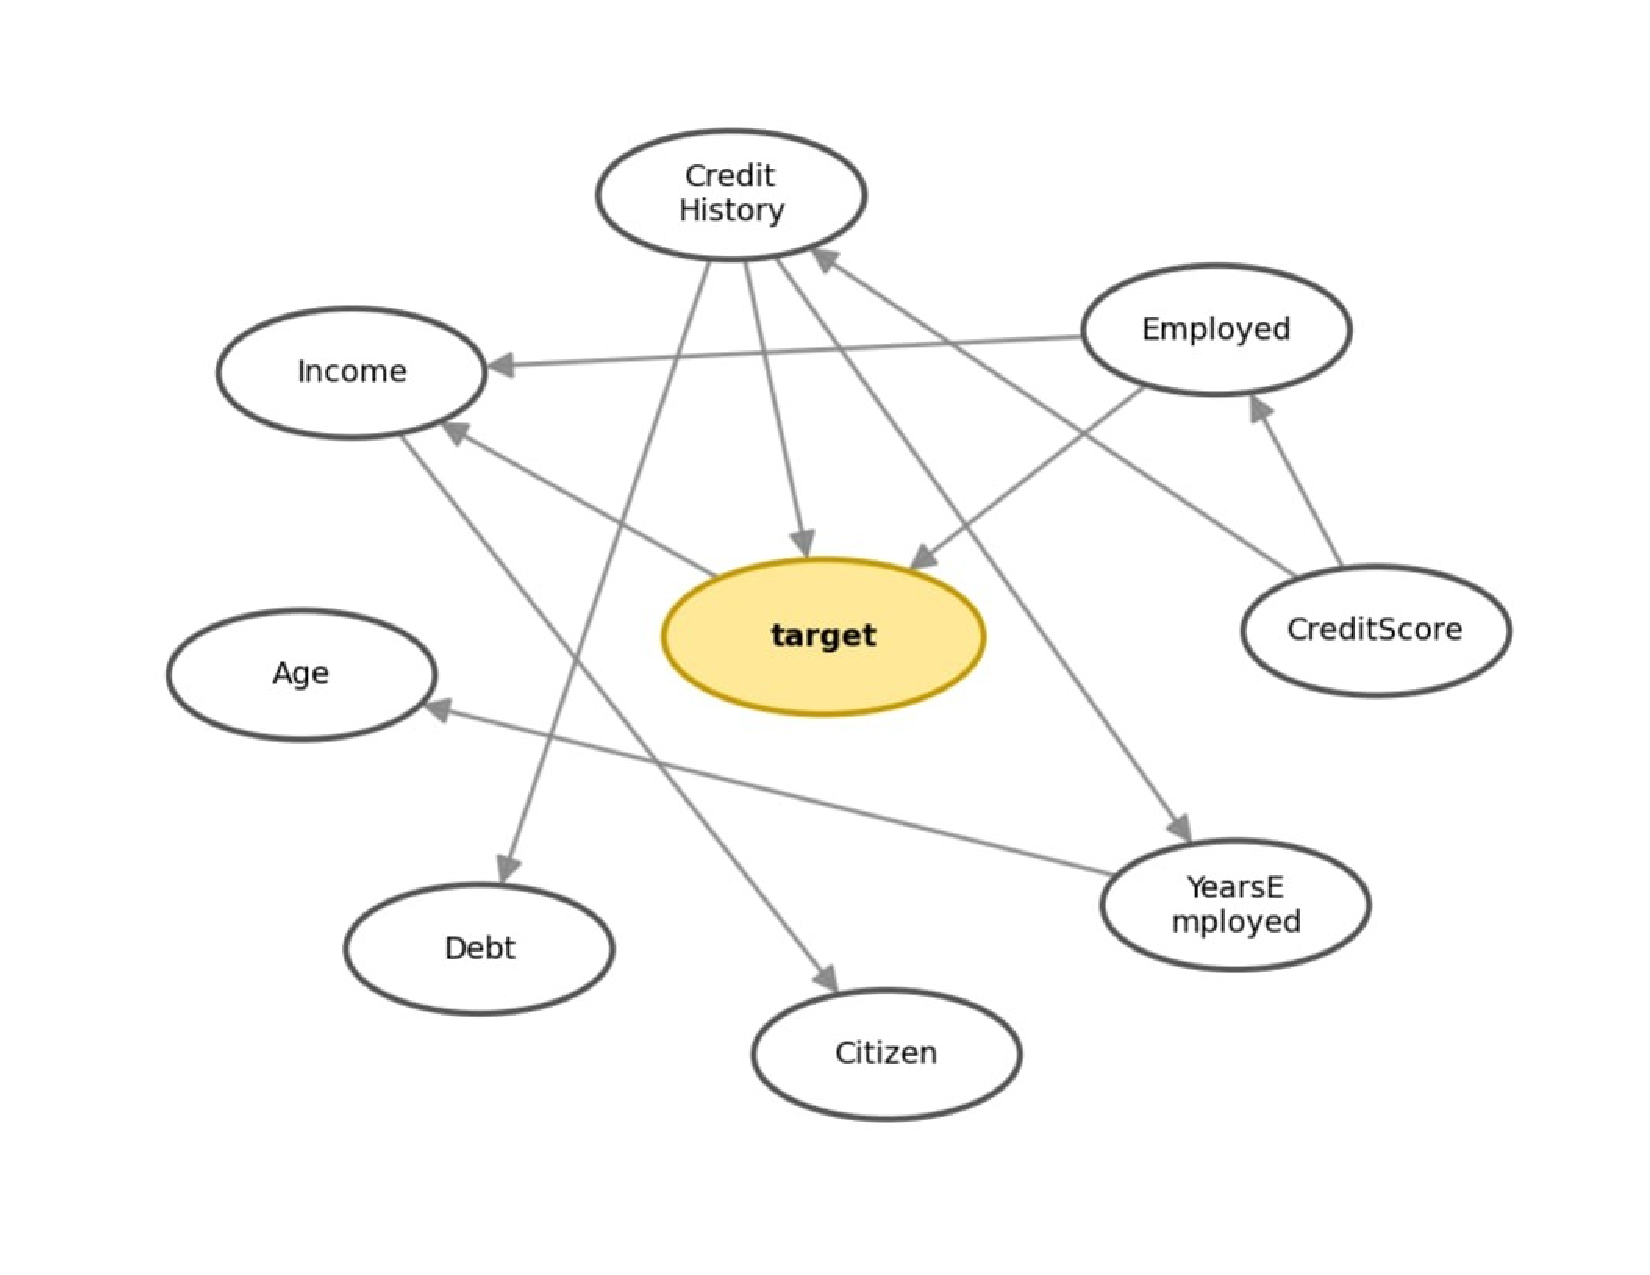
\includegraphics[width=\textwidth,
        height=0.35\textheight,
        trim=2.5cm 2.5cm 2cm 2cm,
        clip]{image/network/graph_au.pdf}
        \caption{Sơ đồ cấu trúc mạng Bayes Australian Credit dataset}
        \label{fig:net_aus}
    \end{subfigure}
    
    \vspace{0.8cm} % Tăng khoảng cách cho thoáng mắt
    % --- HÀNG 1: German Credit ---
    \begin{subfigure}[b]{0.9\textwidth}
        \centering
        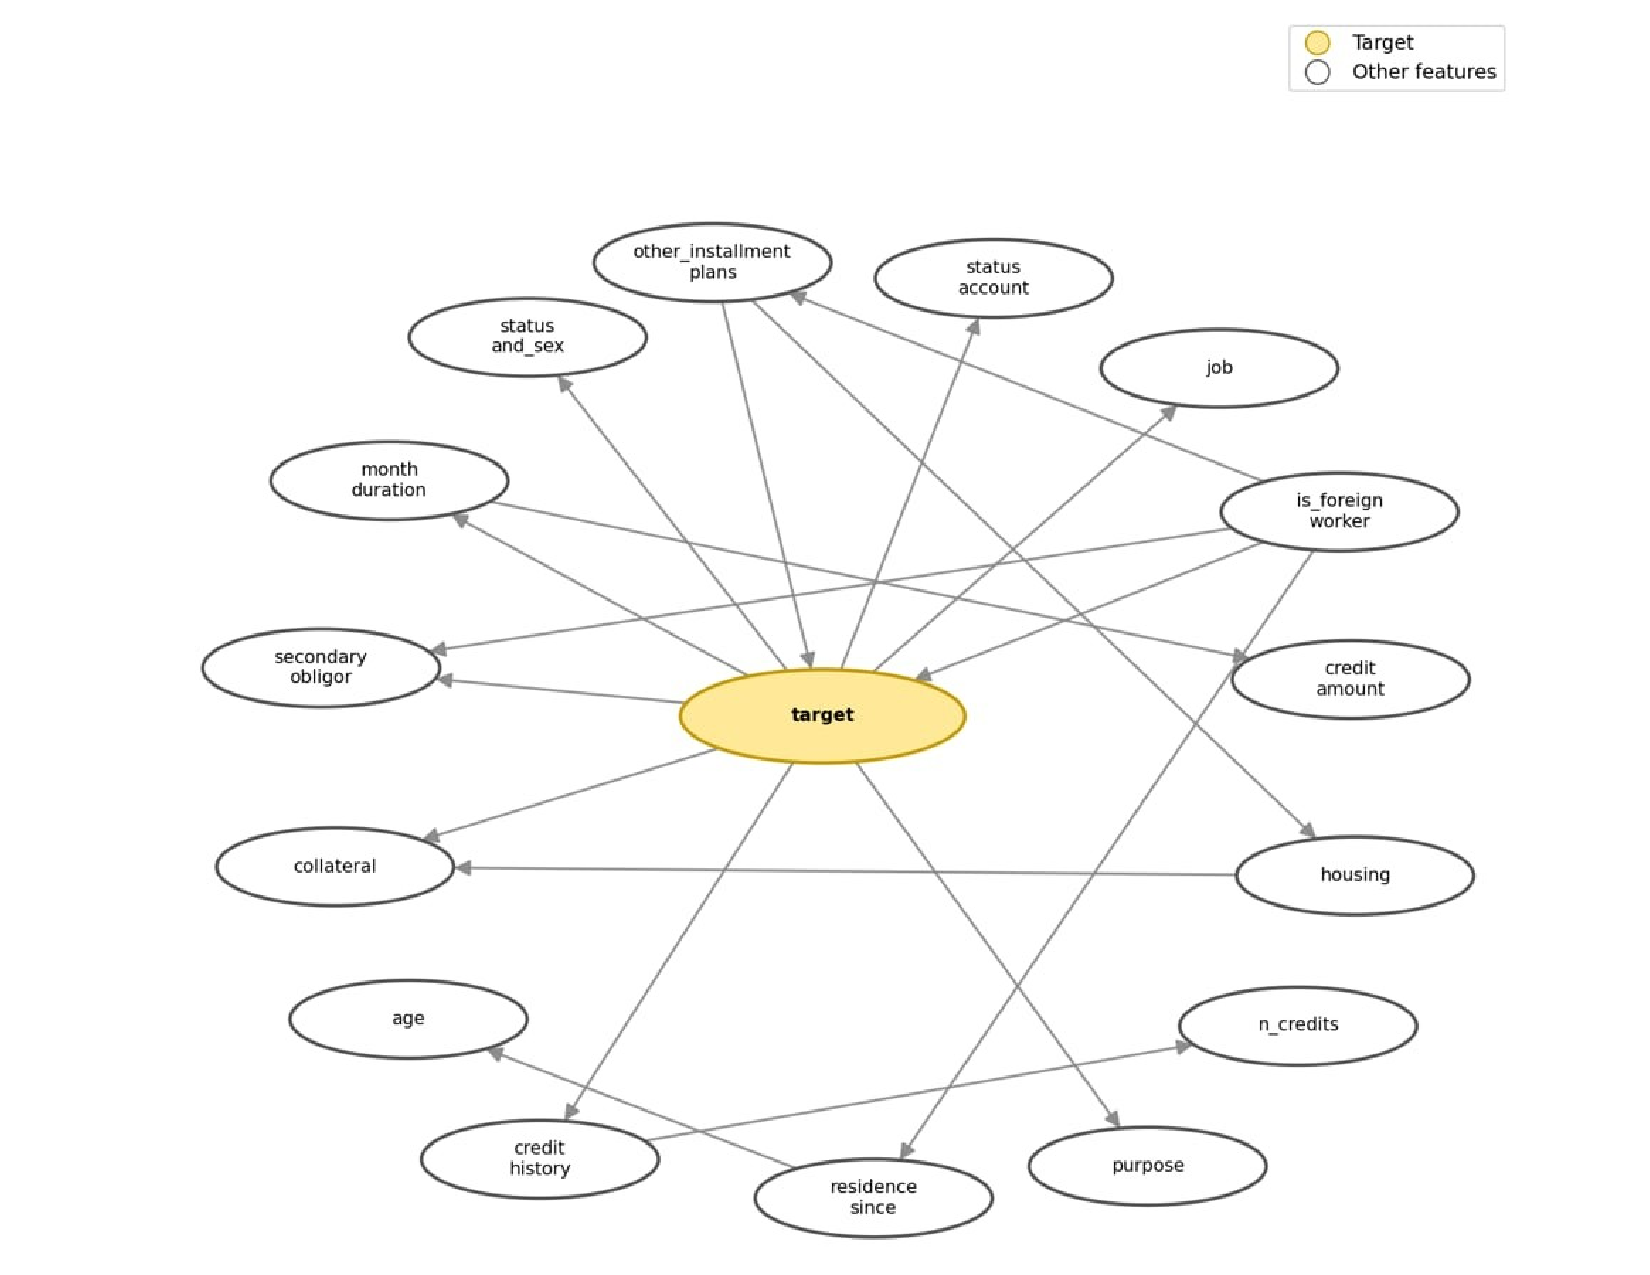
\includegraphics[width=1.1\textwidth,
        height=0.5\textheight,
        trim=2.5cm 0.5cm 2cm 3.5cm,
        clip]{image/network/graph_ger.pdf}
        \caption{Sơ đồ cấu trúc mạng Bayes German Credit dataset}
        \label{fig:net_ger}
    \end{subfigure}

    \caption{Sơ đồ cấu trúc mạng Bayes (Phần 1)}
\end{figure}

\begin{figure}[H]
    \ContinuedFloat % <-- Lệnh quan trọng giúp giữ nguyên số thứ tự Hình (vd: vẫn là Hình 4.5)
    \centering
    
    % --- HÀNG 3: Lending Credit ---
    \begin{subfigure}[b]{1\textwidth}
         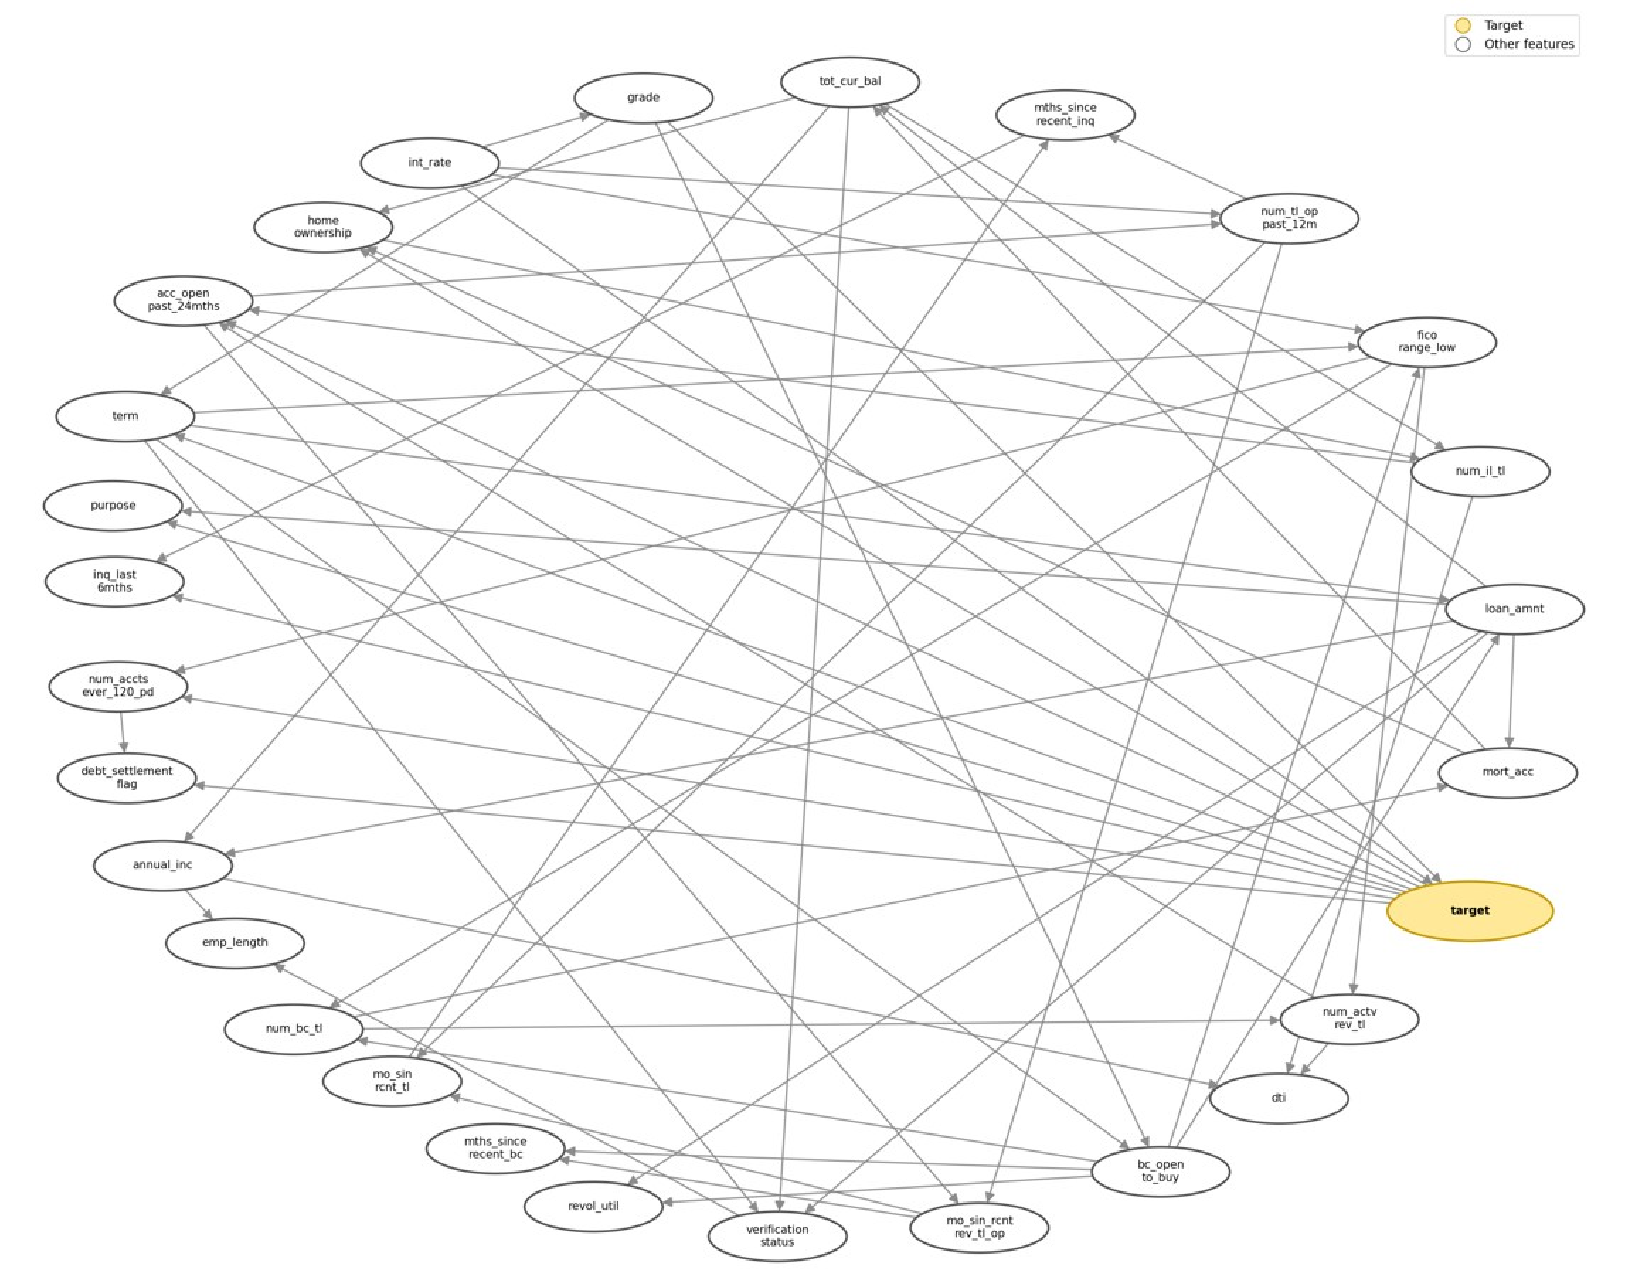
\includegraphics[angle=90,
         width=1.05\textwidth,
        height=1    \textheight,
        trim=0.5cm 0cm 1cm 0.95cm,
        clip]{image/network/graph_lend.pdf}
        \caption{Sơ đồ cấu trúc mạng Bayes Lending Club dataset}
        \label{fig:net_lc}
    \end{subfigure}
    
    \caption{Sơ đồ cấu trúc mạng Bayes (tiếp theo).}
    \label{fig:net}
\end{figure}

\FloatBarrier

Hình \ref{fig:net} cho thấy độ phức tạp cấu trúc đồ thị tỉ lệ thuận với số lượng đặc trưng đầu vào: Lending Club với 27 đặc trưng học được một DAG dày đặc tới 58 cạnh, trong khi Australian Credit chỉ với 8 đặc trưng học được một cấu trúc gọn nhẹ 10 cạnh. Độ ổn định của quá trình tối ưu hóa (đo bằng khoảng dao động điểm BIC giữa 50 lần chạy) cũng khác biệt rõ rệt: ở Australian Credit, biên độ dao động BIC giữa các lần chạy rất hẹp (chỉ khoảng 30 đơn vị quanh giá trị tối ưu), cho thấy không gian tìm kiếm cấu trúc nhỏ và thuật toán Tabu hội tụ rất ổn định và nhất quán giữa các lần khởi tạo ngẫu nhiên khác nhau. Ngược lại, ở Lending Club, biên độ dao động lớn hơn nhiều (hàng nghìn đơn vị BIC), phản ánh không gian cấu trúc rộng và độ nhạy cao với điểm khởi tạo ngẫu nhiên, đây là hệ quả tất yếu của số lượng biến lớn làm không gian DAG khả dĩ tăng theo cấp số nhân (siêu hàm mũ theo số nút).


Trong cả ba cấu trúc học được, biến target có nhiều liên kết trực tiếp (cạnh đến hoặc đi từ target) với các đặc trưng tín dụng cốt lõi, phản ánh đúng trực giác miền (domain knowledge) về rủi ro tín dụng:

\begin{itemize}
    \item Lending Club: target liên kết trực tiếp với int\_rate (lãi suất), grade (xếp hạng tín dụng), debt\_settlement\_flag, num\_accts\_ever\_120\_pd (số tài khoản từng quá hạn 120 ngày), inq\_last\_6mths (số lần truy vấn tín dụng 6 tháng gần nhất), purpose, term, acc\_open\_past\_24mths và home\_ownership.
    
    \item German Credit: target liên kết trực tiếp với status\_account (số dư tài khoản vãng lai), purpose, credit\_history, job, collateral, secondary\_obligor, month\_duration và status\_and\_sex, đồng thời chịu ảnh hưởng trực tiếp từ is\_foreign\_worker và other\_installment\_plans.

    \item Australian Credit: target liên kết trực tiếp và duy nhất với ba biến CreditHistory, Employed và Income, phản ánh cấu trúc nhân quả rất gọn của bộ dữ liệu này.
\end{itemize}

Sự nhất quán giữa cấu trúc đồ thị học được bằng thuật toán dữ liệu thuần túy (data-driven) và kiến thức chuyên gia tín dụng truyền thống (ví dụ lịch sử tín dụng, lãi suất, thu nhập là các yếu tố quyết định) là một chỉ dấu định tính quan trọng cho thấy mô hình BN không chỉ có khả năng dự đoán mà còn có khả năng diễn giải nhân quả hợp lý.

Bên cạnh cấu trúc đồ thị thuần túy, Hình \ref{fig:marginal_australian}, \ref{fig:marginal_german} và \ref{fig:marginal_lendingclub}  trình bày toàn cảnh mạng Bayes của ba bộ dữ liệu kèm theo phân phối biên (marginal distribution) tiên nghiệm của từng node, tức phân phối xác suất của mỗi biến khi chưa có bất kỳ bằng chứng nào được đưa vào, bao gồm cả biến \texttt{target} ở mức 50\%/50\% do đã qua bước cân bằng dữ liệu SMOTE-NC tại $S_{\text{Pro}}$. Cách trực quan hóa này cho phép quan sát đồng thời cả cấu trúc phụ thuộc lẫn hình dạng phân phối của từng biến ngay trên cùng một sơ đồ, thay vì phải tra cứu riêng lẻ từng bảng CPT.

Trên Australian Credit (Hình \ref{fig:marginal_australian}), phân phối biên cho thấy phần lớn khách hàng thuộc nhóm quốc tịch/cư trú state 2 (90.8\%), trong khi \texttt{CreditHistory} và \texttt{Employed} phân bố tương đối cân bằng giữa hai trạng thái (42.9\%/57.1\% và 53.9\%/46.1\%), phản ánh đúng tính chất một bộ dữ liệu đã được xử lý cân bằng nhãn nhưng các đặc trưng đầu vào vẫn giữ nguyên phân phối tự nhiên.

Trên German Credit (Hình \ref{fig:marginal_german}), đáng chú ý là \texttt{is\_foreign\_worker} lệch mạnh về state 1 (83.0\%) và \texttt{secondary\_obligor} lệch mạnh về state 2 "guarantor" (73.2\%), cho thấy đây là hai đặc trưng có phân phối tự nhiên mất cân bằng rõ rệt trong tổng thể dữ liệu, một yếu tố cần lưu ý khi diễn giải các kết quả suy luận tiến/lùi liên quan đến hai biến này ở Mục \ref{sec:4.4.1} và \ref{sec:4.4.2}, vì các trạng thái thiểu số (\texttt{is\_foreign\_worker}=0, \texttt{secondary\_obligor}$\in\{0,1\}$) vốn dĩ đã có ít quan sát hỗ trợ ngay từ đầu.

Trên Lending Club (Hình \ref{fig:marginal_lendingclub}), \texttt{debt\_settlement\_flag} lệch cực mạnh về state 0 (98\%), chỉ 2\% khách hàng từng tham gia chương trình tái cơ cấu nợ, đây chính là gốc rễ của hiện tượng dữ liệu thưa khi biến này liên tục cho ra các giá trị xác suất cực trị ($\delta=0.5$, hoặc xác suất hậu nghiệm bão hòa 100\%). Tương tự, \texttt{num\_accts\_ever\_120\_pd} cũng lệch mạnh về state 0 (73.1\%). Việc quan sát trước phân phối biên như vậy giúp lý giải có cơ sở cho các kết quả bất thường xuất hiện xuyên suốt phần thực nghiệm diễn giải mô hình ở các mục sau, thay vì phải suy đoán ngược lại từ kết quả.

\vspace{1em}
\begin{table}[ht]
\centering
\caption{Tổng hợp chỉ số đánh giá mô hình mạng Bayes trên tập huấn luyện và tập kiểm tra}
\label{tab:bn_train_test}

\renewcommand{\arraystretch}{1.3}

\begin{tabular}{|
p{2.5cm}|
>{\centering\arraybackslash}p{1.5cm}|
>{\centering\arraybackslash}p{1.5cm}|
>{\centering\arraybackslash}p{1.5cm}|
>{\centering\arraybackslash}p{1.5cm}|
>{\centering\arraybackslash}p{1.5cm}|
>{\centering\arraybackslash}p{1.5cm}|}

\hline
\rowcolor{gray!20}

\makecell{\centering \textcolor{black}{\textbf{Chỉ số}}} &
\multicolumn{2}{c|}{\textcolor{black}{\textbf{Lending Club}}} &
\multicolumn{2}{c|}{\textcolor{black}{\textbf{German Credit}}} &
\multicolumn{2}{c|}{\textcolor{black}{\textbf{Australian Credit}}} \\

\cline{2-7}

\rowcolor{gray!20}
&
\multicolumn{1}{>{\columncolor{gray!20}}c|}{\textcolor{black}{\textbf{Train}}} &
\multicolumn{1}{>{\columncolor{gray!20}}c|}{\textcolor{black}{\textbf{Test}}} &
\multicolumn{1}{>{\columncolor{gray!20}}c|}{\textcolor{black}{\textbf{Train}}} &
\multicolumn{1}{>{\columncolor{gray!20}}c|}{\textcolor{black}{\textbf{Test}}} &
\multicolumn{1}{>{\columncolor{gray!20}}c|}{\textcolor{black}{\textbf{Train}}} &
\multicolumn{1}{>{\columncolor{gray!20}}c|}{\textcolor{black}{\textbf{Test}}} \\

\hline

Accuracy
& 0.7085 & 0.6808
& 0.7811 & 0.7300
& 0.8641 & 0.8406 \\

\hline

Precision
& 0.7269 & 0.4610
& 0.8386 & 0.6047
& 0.9247 & 0.9211 \\

\hline

Recall 
& 0.6679 & 0.4878
& 0.6962 & 0.4127
& 0.7926 & 0.8140 \\

\hline

Specificity
& 0.7490 & 0.7615
& 0.8660 & 0.8759
& 0.9355 & 0.8846 \\

\hline

F1-Score
& 0.7034 & 0.4740
& 0.7608 & 0.4906
& 0.8536 & 0.8642 \\


\hline

ROC-AUC
& 0.7944 & 0.6910
& 0.8686 & 0.7667
& 0.9278 & 0.9220 \\

\hline

PR-AUC
& 0.8238 & 0.5224
& 0.8886 & 0.5421
& 0.9070 & 0.9371 \\

\hline

\end{tabular}
\end{table}
\FloatBarrier

\vspace{1em}
Kết quả ở Bảng \ref{tab:bn_train_test} cho thấy một xu hướng rõ rệt: hiệu năng dự đoán của mô hình BN tăng dần theo chiều Lending Club $\rightarrow$ German Credit $\rightarrow$ Australian Credit, với ROC-AUC lần lượt là 0.6910, 0.7667 và 0.9220. Điều này có thể được lý giải từ ba góc độ. Mức độ nhiễu nội tại của dữ liệu, Lending Club là dữ liệu cho vay tiêu dùng thực tế quy mô lớn với hành vi vỡ nợ phụ thuộc vào nhiều yếu tố ngẫu nhiên ngoài hồ sơ tín dụng (thất nghiệp đột xuất, biến động kinh tế vĩ mô...), trong khi German và Australian Credit là dữ liệu chuẩn hóa cao của UCI, vốn đã qua xử lý và có quan hệ đặc trưng, nhãn rõ ràng hơn. Độ phức tạp số chiều, số đặc trưng càng nhiều (27 so với 8) thì không gian CPT của mạng Bayes càng phức tạp, dễ dẫn đến hiện tượng dữ liệu thưa (data sparsity) trong các bảng xác suất có điều kiện và làm giảm độ chính xác ước lượng tham số. Đối với Australian Credit, do prevalence của nhãn default cao ($\approx 58 \%$), bài toán phân loại có phần dễ hơn về mặt thống kê khi không phải đối mặt với độ mất cân bằng cực đoan trên tập test.

Trên bộ Lending Club, AUC trên tập train đạt 0.7944 trong khi AUC trên tập test chỉ đạt 0.6910, mức chênh lệch khá lớn ($\approx 0.1034$), cho thấy mô hình có dấu hiệu overfitting nhẹ đến trung bình đối với cấu trúc đồ thị 58 cạnh học được từ 27 biến. Đây là hệ quả hợp lý của việc mạng Bayes rời rạc với CPT có số tổ hợp trạng thái lớn (do nhiều biến và nhiều cạnh) dễ khớp quá mức với phân phối thực nghiệm của tập huấn luyện. Đối với Australian Credit có cấu trúc gọn hơn, ít cạnh hơn, khoảng cách train–test được kỳ vọng hẹp hơn đáng kể do số bậc tự do (degrees of freedom) của mô hình thấp hơn nhiều so với cỡ mẫu.

\begin{figure}[h]
\centering
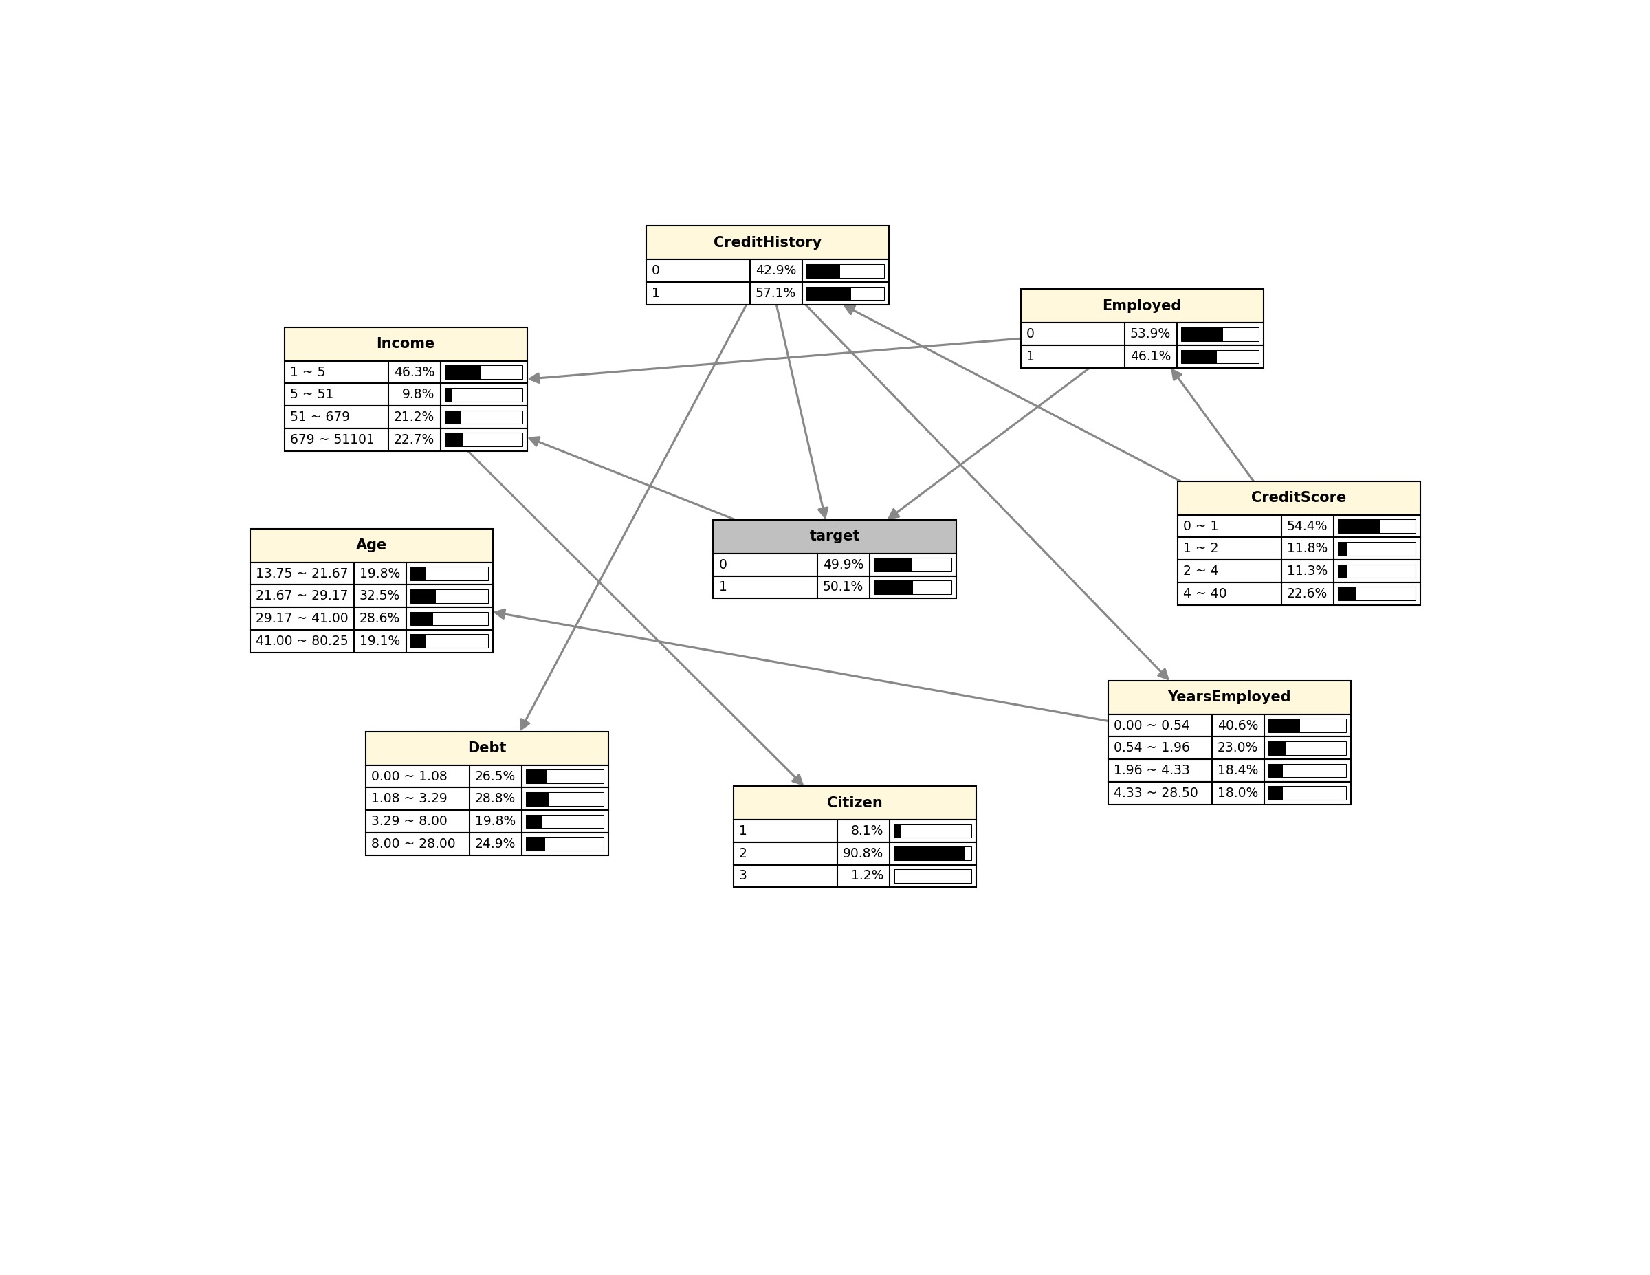
\includegraphics[
    width=1.05\textwidth,
    height=0.6\textheight,
    trim=3cm 5cm 3cm 3cm,
    clip
]{image/au_back.pdf}
\caption{Phân phối xác suất của toàn mạng --- Australian Credit}
\label{fig:marginal_australian}
\end{figure}

\begin{figure}[h]
\centering
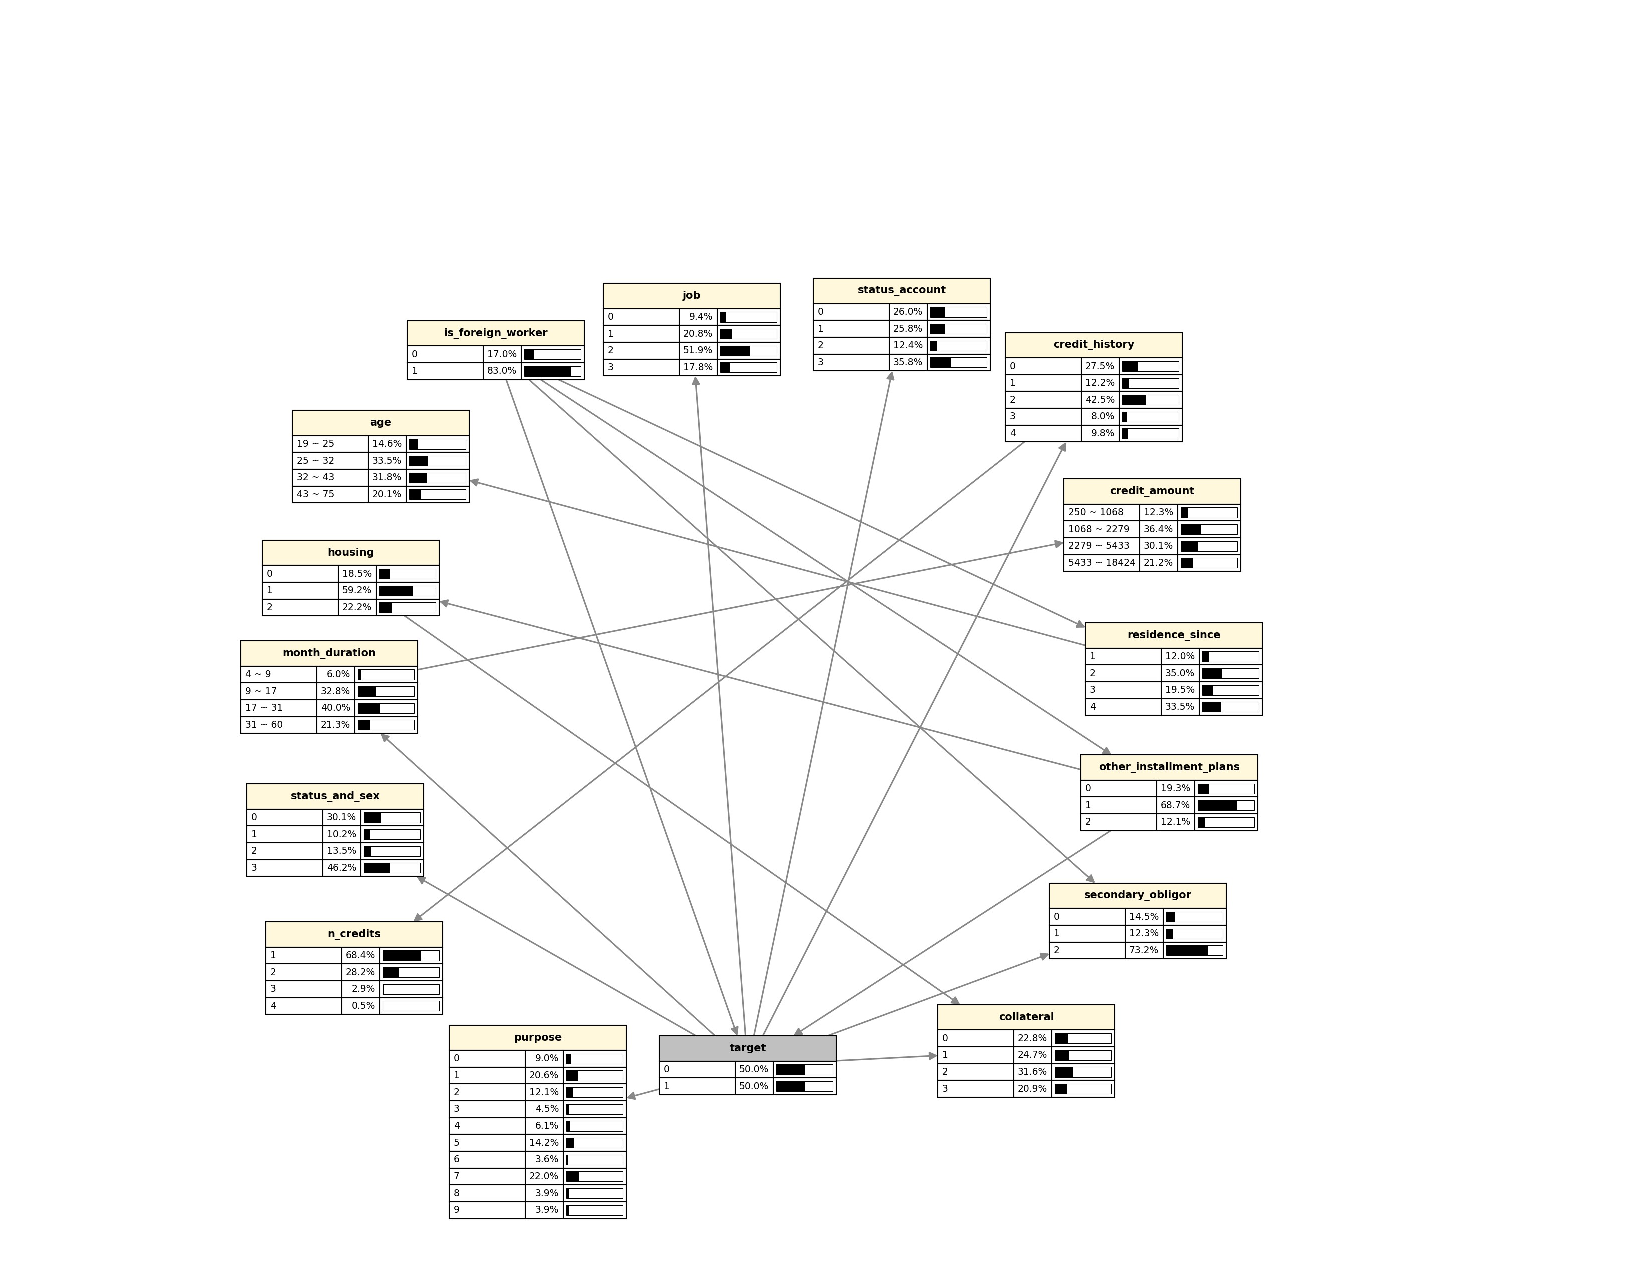
\includegraphics[
    width=1.2\textwidth,
    height=0.8\textheight,
    trim=3cm 0.5cm 3cm 3cm,
    clip
]{image/ger_back.pdf}
\caption{Phân phối xác suất của toàn mạng --- German Credit}
\label{fig:marginal_german}
\end{figure}

\begin{figure}[h]
\centering
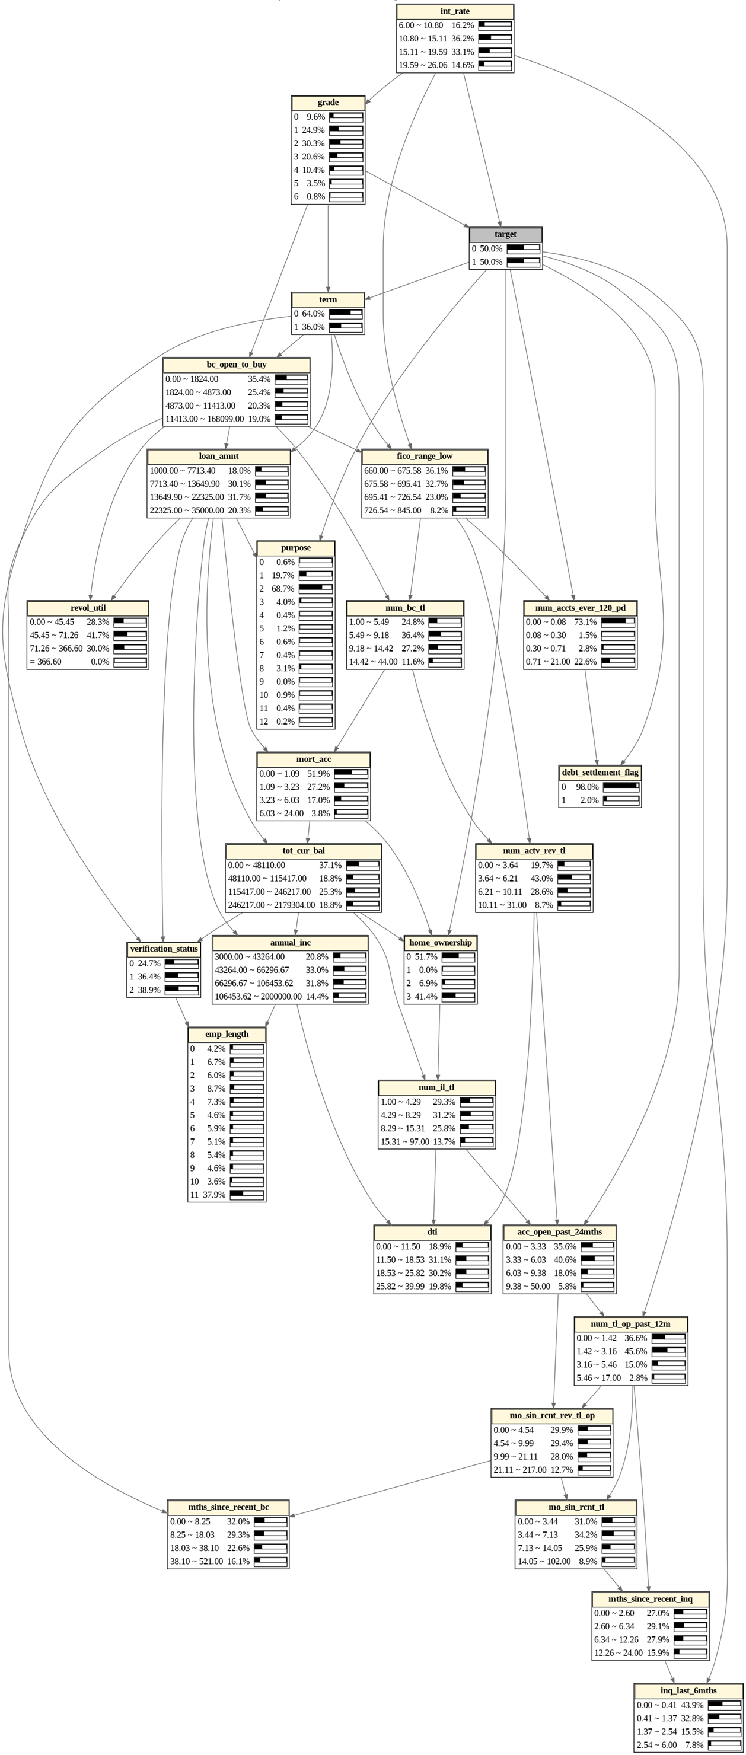
\includegraphics[width=1.1\textwidth,height=\textheight]{image/lend_back.pdf}
\caption{Phân phối xác suất của toàn mạng --- Lending Club}
\label{fig:marginal_lendingclub}
\end{figure}

\FloatBarrier
\subsubsection{Phân tích đường cong ROC, ngưỡng tối ưu và Decision Curve Analysis trên tập Validation}

\noindent
\textbf{\textit{Australian Credit}}

\begin{figure}[H]
    \centering
    \begin{subfigure}[b]{0.7\textwidth} % Giảm nhẹ xuống 0.8 để 2 hình chắc chắn vừa 1 trang
        \centering
        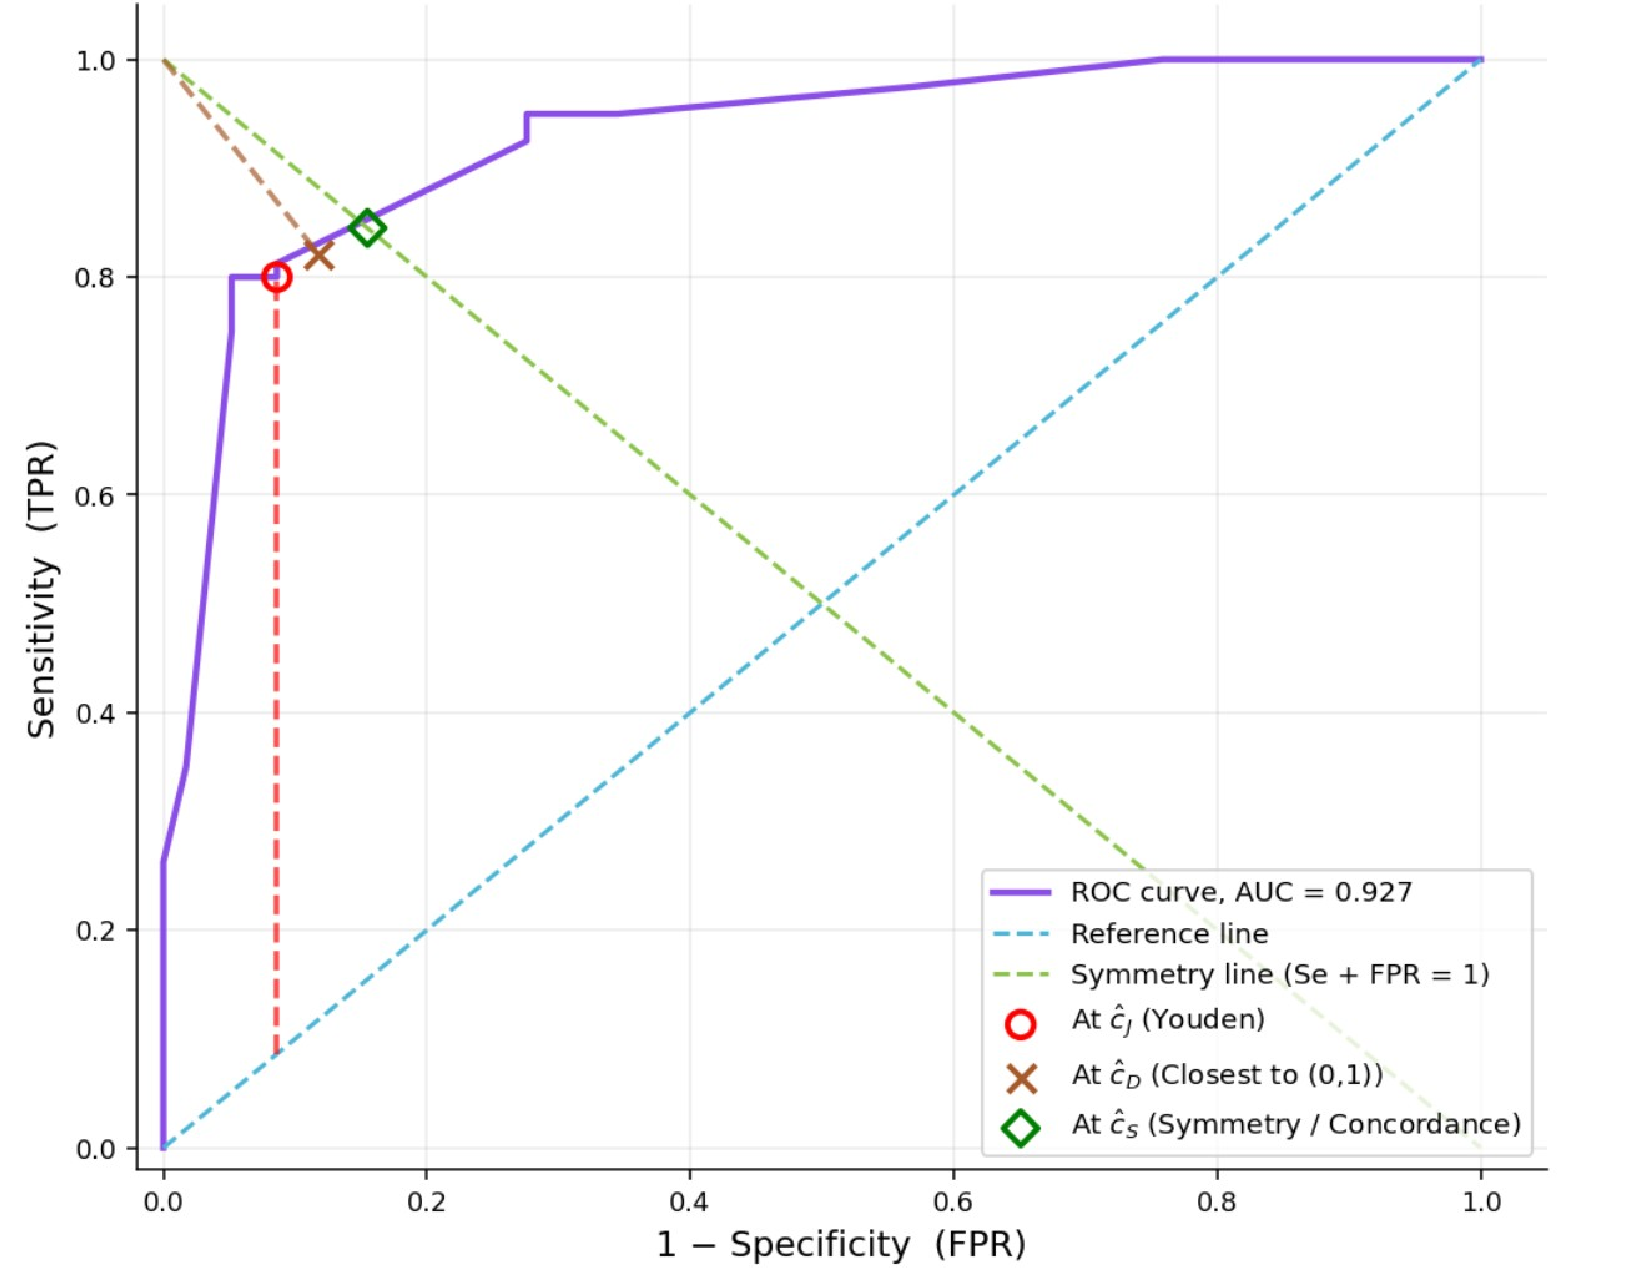
\includegraphics[width=\textwidth]{image/roc_dca/roc_au.pdf}
    \end{subfigure}
    \caption{Đồ thị ba ngưỡng quyết định tối ưu theo ROC --- Australian Credit}
    \label{fig:roc_au}
\end{figure}

\begin{figure}[H]
    \centering
    \begin{subfigure}[b]{0.7\textwidth}
        \centering
        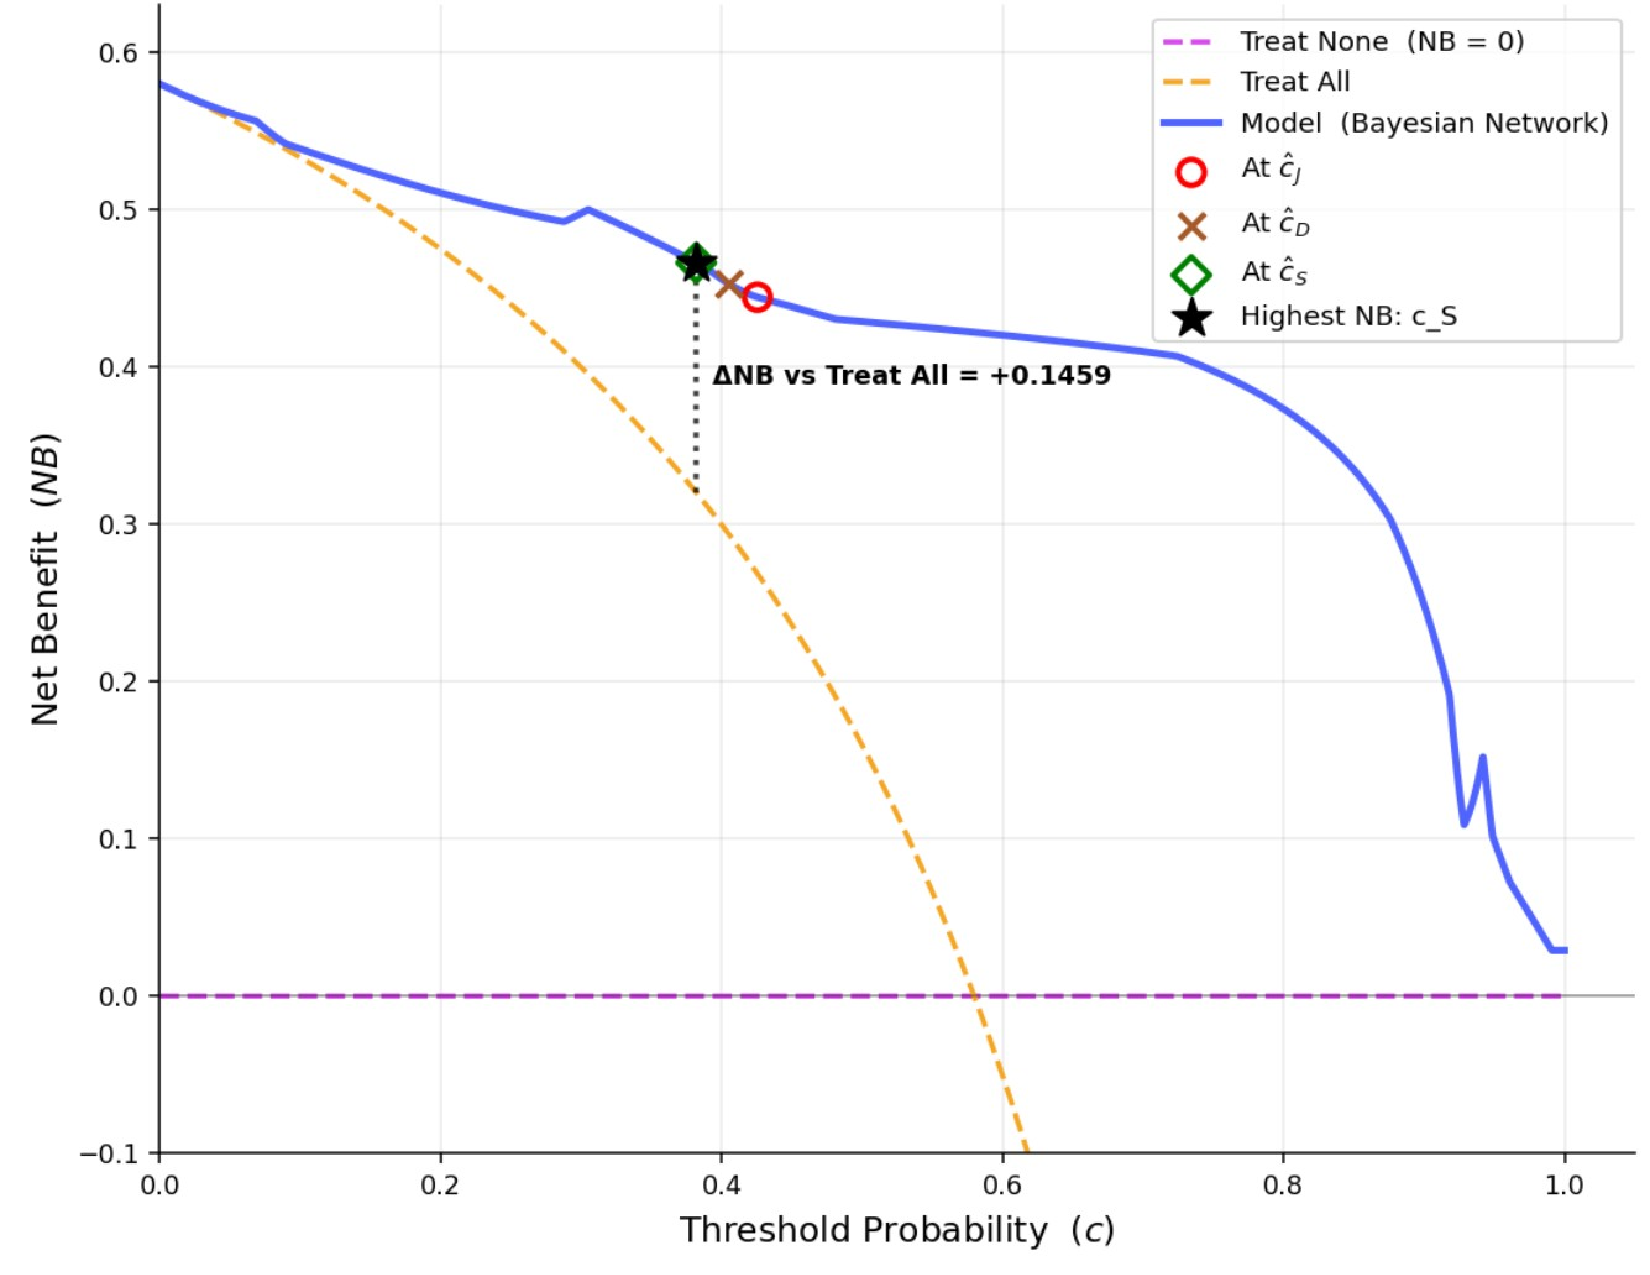
\includegraphics[width=\textwidth]{image/roc_dca/dca_au.pdf}
    \end{subfigure}
    \caption{Đồ thị ba ngưỡng quyết định tối ưu trên DCA --- Australian Credit}
    \label{fig:dca_au}
\end{figure}

\begin{table}[H]
\centering
\caption{Ba ngưỡng quyết định tối ưu theo ROC -- Australian Credit (tập validation)}
\label{tab:roc_threshold}

\renewcommand{\arraystretch}{1.3}

\begin{tabular}{|p{4cm}|c|c|c|c|c|}
\hline
\rowcolor{gray!20}
\centering\textbf{Tiêu chí ngưỡng} &
\centering\textbf{Ngưỡng (c)} &
\centering\textbf{Sensitivity} &
\centering\textbf{Specificity} &
\centering\textbf{Accuracy} &
\centering\arraybackslash\textbf{F1-Score} \\
\hline

Youden Index &
0.4254 &
0.8125 &
0.9138 &
0.8551 &
0.8667 \\
\hline

Closest to (0,1) &
0.4052 &
0.8125 &
0.9138 &
0.8551 &
0.8667 \\
\hline

Symmetry Point &
0.3818 &
0.9250 &
0.7241 &
0.8406 &
0.8706 \\
\hline

\end{tabular}
\end{table}

Kết quả DCA dựa vào Hình \ref{fig:roc_au}, \ref{fig:dca_au} và Bảng \ref{tab:roc_threshold}: với prevalence = 0.5797, Ngưỡng Symmetry Point ($c_S = 0.3818$) cho Net Benefit cao nhất trong ba ngưỡng (NB = 0.4661), vượt Treat All 0.1459 điểm.

\vspace{1em}
\noindent
\textbf{\textit{German Credit}}

Kết quả DCA dựa vào Hình \ref{fig:roc_ger}, \ref{fig:dca_ger} và Bảng \ref{tab:roc_threshold_german}: prevalence (tỉ lệ default) trên tập validation = 0.2750. Trong ba ngưỡng ROC tối ưu, ngưỡng Closest-to (0,1) ($c_D = 0.1895$) cho Net Benefit cao nhất (NB = 0.1474), vượt Treat All 0.0419 điểm Net Benefit.

\begin{figure}[H]
    \centering
    \begin{subfigure}[b]{0.85\textwidth} % Giảm nhẹ xuống 0.8 để 2 hình chắc chắn vừa 1 trang
        \centering
        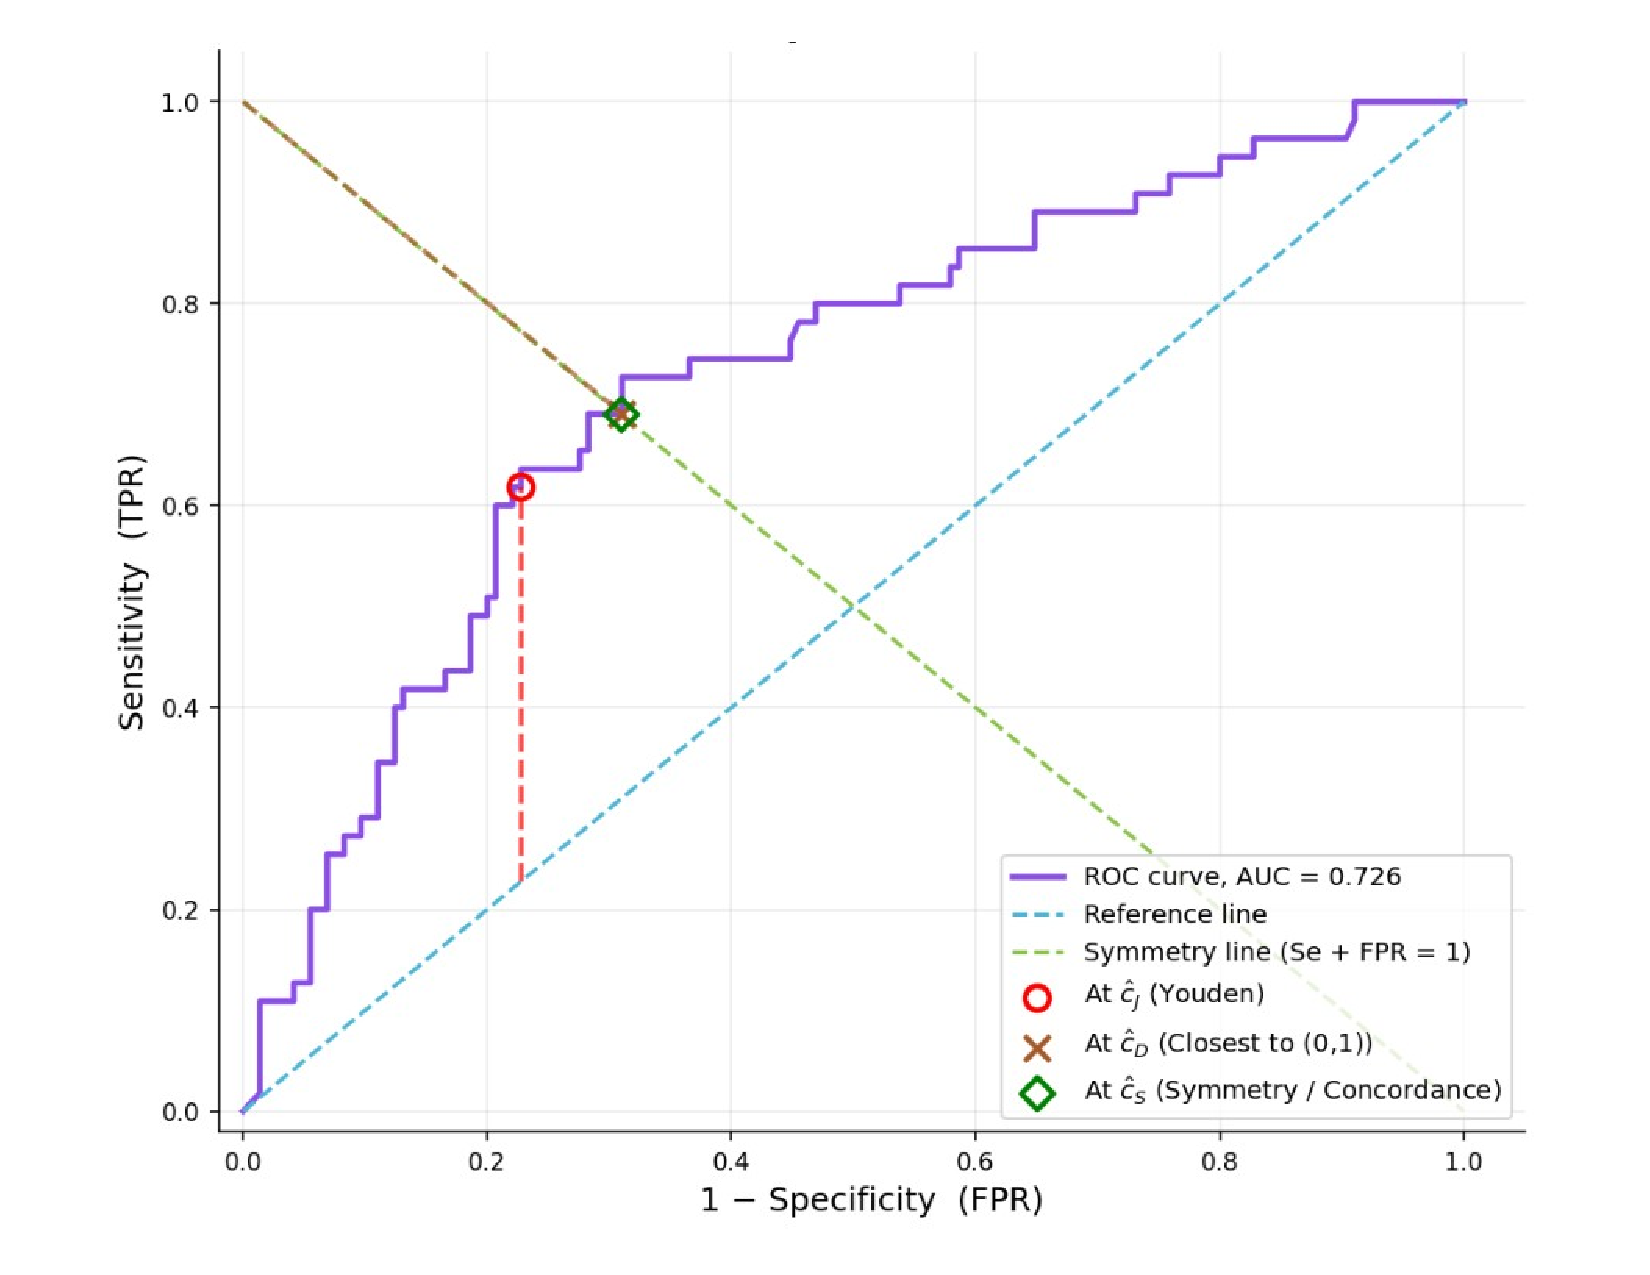
\includegraphics[width=\textwidth]{image/roc_dca/roc_ger.pdf}
    \end{subfigure}
    \caption{Đồ thị ba ngưỡng quyết định tối ưu theo ROC --- German Credit}
    \label{fig:roc_ger}
\end{figure}

\begin{figure}[H]
    \centering
    \begin{subfigure}[b]{0.85\textwidth}
        \centering
        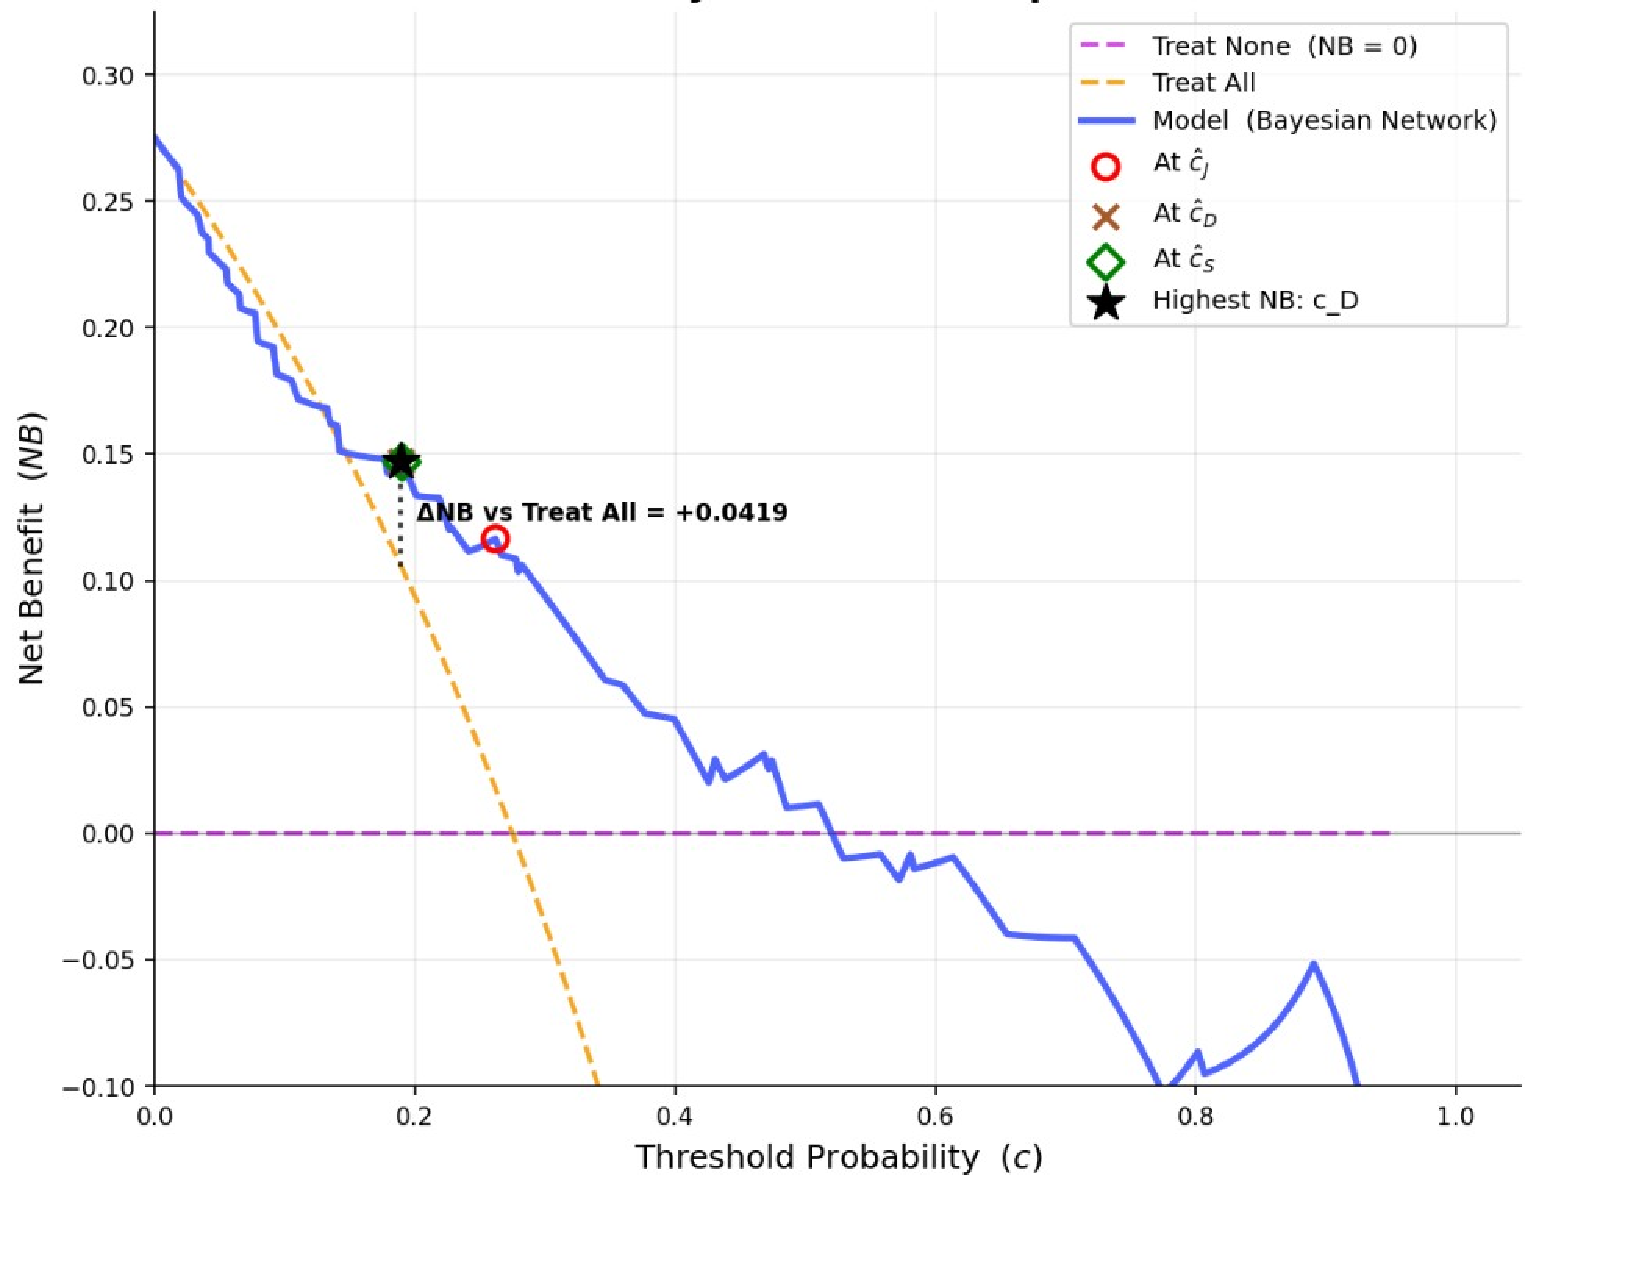
\includegraphics[width=\textwidth]{image/roc_dca/dca_ger.pdf}
    \end{subfigure}
    \caption{Đồ thị ba ngưỡng quyết định tối ưu trên DCA --- German Credit}
    \label{fig:dca_ger}
\end{figure}

\begin{table}[H]
\centering
\caption{Ba ngưỡng quyết định tối ưu theo ROC -- German Credit (tập validation)}
\label{tab:roc_threshold_german}

\renewcommand{\arraystretch}{1.3}

\begin{tabular}{|p{4cm}|c|c|c|c|c|}
\hline
\rowcolor{gray!20}
\centering\textbf{Tiêu chí ngưỡng} &
\centering\textbf{Ngưỡng (c)} &
\centering\textbf{Sensitivity} &
\centering\textbf{Specificity} &
\centering\textbf{Accuracy} &
\centering\arraybackslash\textbf{F1-Score} \\
\hline

Youden Index
& 0.2619
& 0.6364
& 0.7724
& 0.7350
& 0.5691 \\
\hline

Closest to (0,1)
& 0.1895
& 0.7091
& 0.6897
& 0.6950
& 0.5612 \\
\hline

Symmetry Point
& 0.1901
& 0.7091
& 0.6897
& 0.6950
& 0.5612 \\
\hline

\end{tabular}
\end{table}

\vspace{1em}
\noindent
\textbf{\textit{Lending Club}}

Kết quả DCA Hình \ref{fig:roc_lend}, \ref{fig:dca_lend} và Bảng \ref{tab:roc_threshold_lending}: prevalence = 0.3017. Đáng chú ý, cả ba ngưỡng đều có Net Benefit của Treat All âm, nên baseline so sánh là Treat None (NB = 0); ngưỡng Youden ($c_J = 0.3431$) cho Net Benefit dương cao nhất trong ba ngưỡng (NB = 0.0561) nhưng ở mức thấp hơn đáng kể so với hai bộ dữ liệu còn lại, cho thấy lợi ích thực tiễn của mô hình BN trên Lending Club hạn chế hơn.

\begin{figure}[H]
    \centering
    \begin{subfigure}[b]{0.85\textwidth} % Giảm nhẹ xuống 0.8 để 2 hình chắc chắn vừa 1 trang
        \centering
        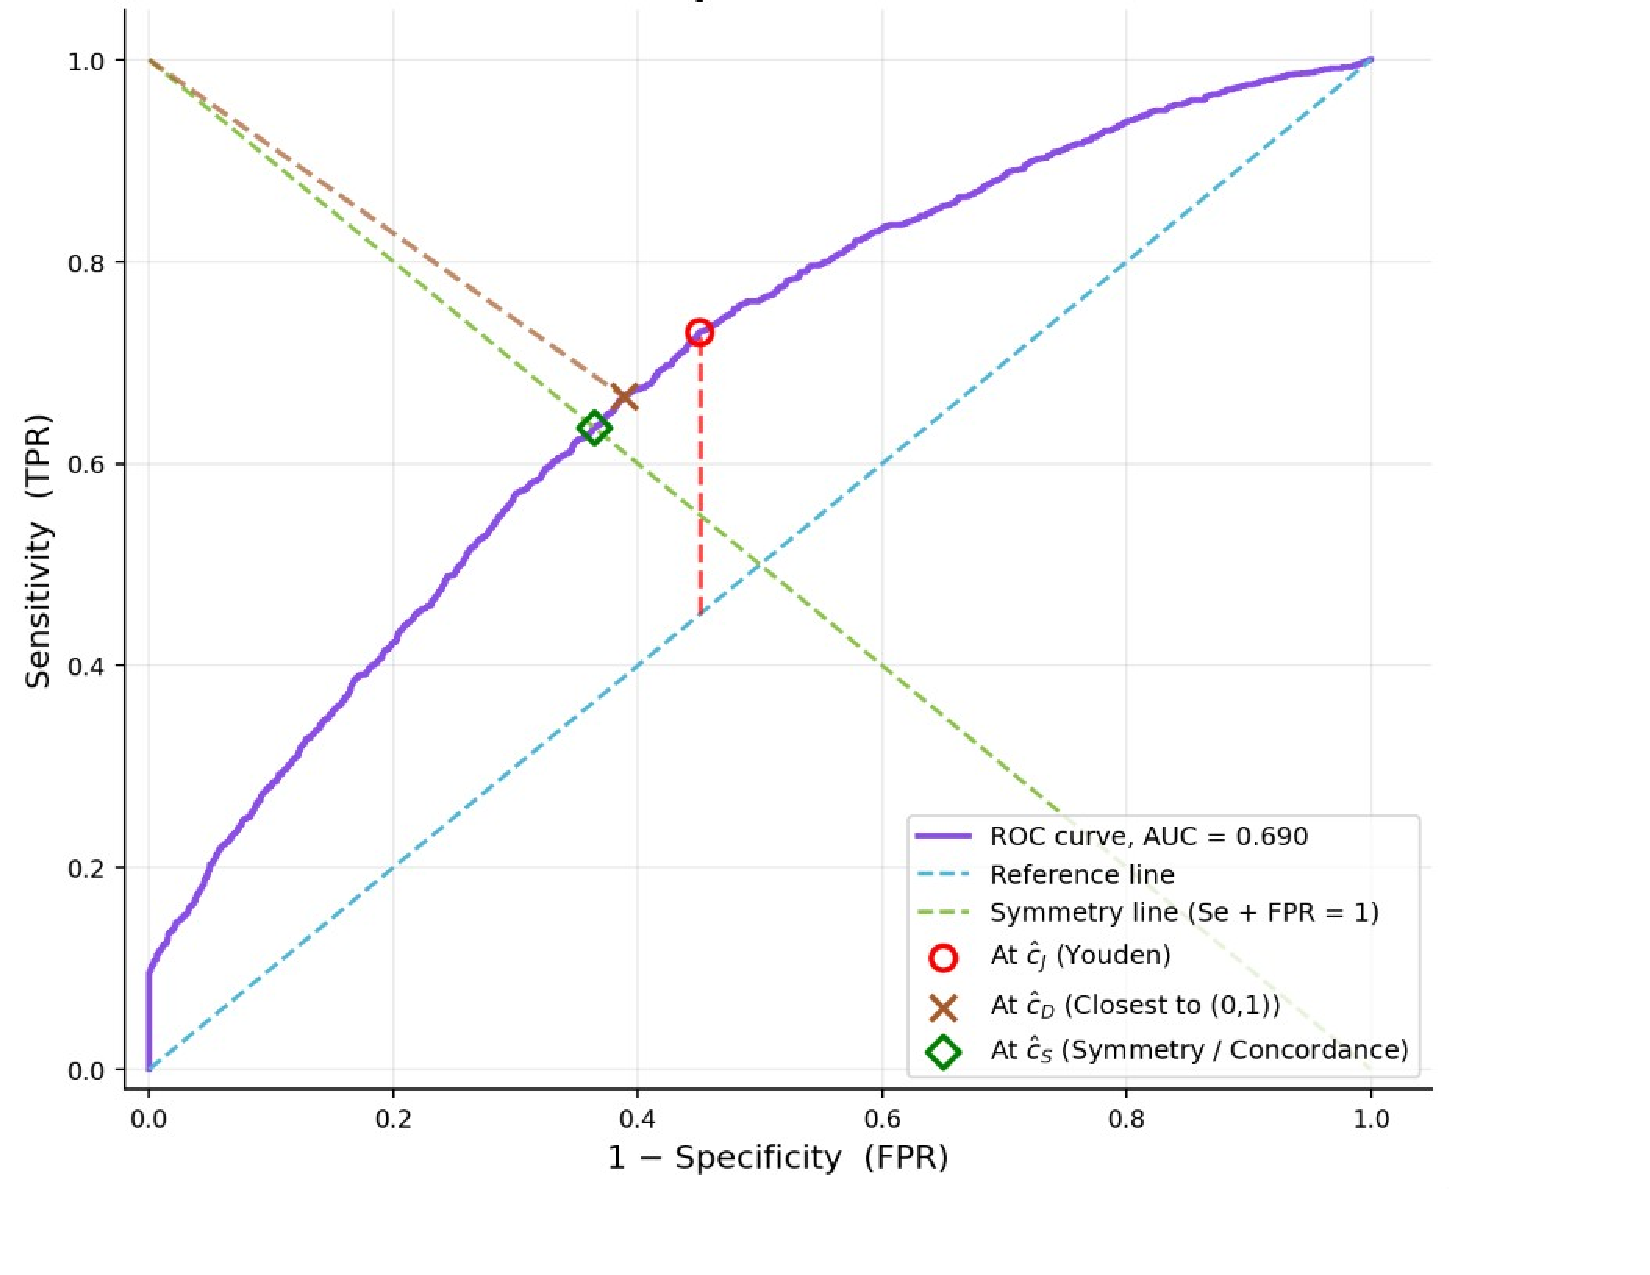
\includegraphics[width=\textwidth]{image/roc_dca/roc_lend.pdf}
    \end{subfigure}
    \caption{Đồ thị ba ngưỡng quyết định tối ưu theo ROC --- Lending Club}
    \label{fig:roc_lend}
\end{figure}

\begin{figure}[H]
    \centering
    \begin{subfigure}[b]{0.85\textwidth}
        \centering
        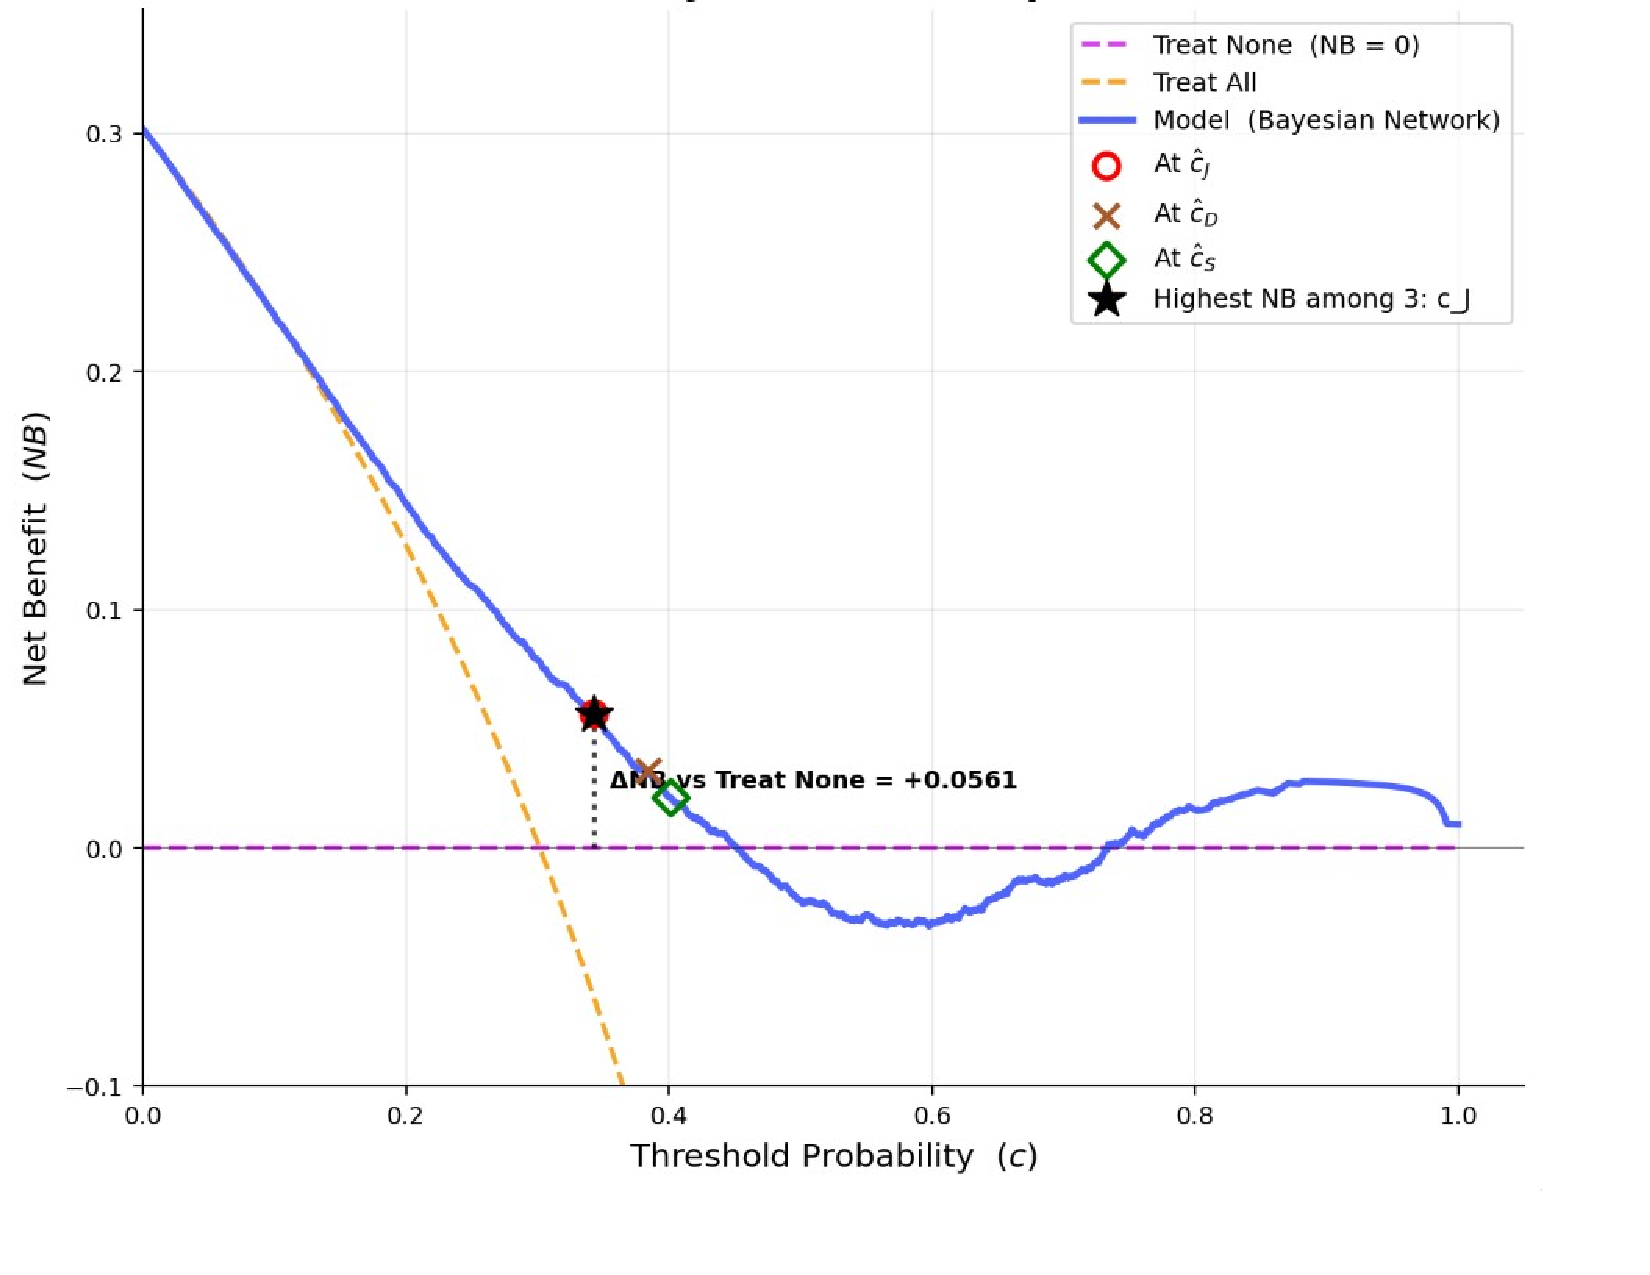
\includegraphics[width=\textwidth]{image/roc_dca/dca_lend.pdf}
    \end{subfigure}
    \caption{Đồ thị ba ngưỡng quyết định tối ưu trên DCA --- Lending Club}
    \label{fig:dca_lend}
\end{figure}

\begin{table}[H]
\centering
\caption{Ba ngưỡng quyết định tối ưu theo ROC -- Lending Club (tập validation)}
\label{tab:roc_threshold_lending}

\renewcommand{\arraystretch}{1.3}

\begin{tabular}{|p{3.5cm}|c|c|c|c|c|}
\hline
\rowcolor{gray!20}
\centering\textbf{Tiêu chí ngưỡng} &
\centering\textbf{Ngưỡng (c)} &
\centering\textbf{Sensitivity} &
\centering\textbf{Specificity} &
\centering\textbf{Accuracy} &
\centering\arraybackslash\textbf{F1-Score} \\
\hline

Youden Index
& 0.3593
& 0.7232
& 0.5313
& 0.5892
& 0.5151 \\
\hline

Closest to (0,1)
& 0.4016
& 0.6403
& 0.6098
& 0.6190
& 0.5035 \\
\hline

Symmetry Point
& 0.4088
& 0.6227
& 0.6227
& 0.6227
& 0.4989 \\
\hline

\end{tabular}
\end{table}
\FloatBarrier

\noindent
Trên bộ Lending Club, khi hạ ngưỡng quyết định từ 0.5 mặc định xuống mức tối ưu theo Youden ($\approx$ 0.3593) làm tăng đáng kể độ nhạy (từ 0.4878 lên 0.7232) nhưng đồng thời làm giảm độ đặc hiệu và độ chính xác tổng thể,  là sự đánh đổi kinh điển (trade-off) giữa việc phát hiện nhiều khách hàng vỡ nợ hơn (giảm rủi ro bỏ sót  FN) với chi phí từ chối oan nhiều khách hàng tốt hơn (tăng FP). Trên Australian Credit, do mô hình đã đạt hiệu năng cao ở ngưỡng mặc định, nên ở ngưỡng tối ưu Youden và Closest-to (0,1) mô hình có hiệu năng trùng khớp nhau hoàn toàn (0.4254 $\approx$ 0.4052, cùng cho Accuracy 0.8551), cho thấy đường cong ROC của bộ dữ liệu này có hình dạng rất gần góc trên bên trái, cho thấy đặc trưng của một bộ phân loại mạnh.

Mô hình BN cho lợi ích ròng dương trên cả ba bộ dữ liệu trong vùng ngưỡng xác suất thấp đến trung bình, vượt trội hơn cả hai chiến lược biên, chứng minh giá trị triển khai thực tiễn của mô hình ngoài giá trị thống kê thuần túy. Đáng chú ý, Net Benefit tuyệt đối tại Australian Credit (0.4661) cao hơn rất nhiều so với German Credit (0.1474) và Lending Club (0.0561), phản ánh trực tiếp hiệu năng phân loại vượt trội của mô hình trên bộ dữ liệu này (ROC-AUC = 0.9220), đồng thời cũng phản ánh prevalence cao hơn (0.58) làm tăng quy mô tuyệt đối của lợi ích ròng có thể đạt được. Sự thay đổi của các chỉ số khi áp dụng các ngưỡng tối ưu trên ba bộ dữ liệu được phản ánh trong Bảng \ref{tab:bn_best_c}.

\vspace{1em}
\begin{table}[ht]
\centering
\caption{So sánh chỉ số đánh giá mô hình mạng Bayes với ngưỡng tối ưu trên tập test}
\label{tab:bn_best_c}

\renewcommand{\arraystretch}{1.3}

\begin{tabular}{|
p{2cm}|
>{\centering\arraybackslash}p{1.2cm}|
>{\centering\arraybackslash}p{2cm}|
>{\centering\arraybackslash}p{1.2cm}|
>{\centering\arraybackslash}p{2cm}|
>{\centering\arraybackslash}p{1.2cm}|
>{\centering\arraybackslash}p{2cm}|}

\hline
\rowcolor{gray!20}

\makecell{\centering \textcolor{black}{\textbf{Chỉ số}}} &
\multicolumn{2}{c|}{\textcolor{black}{\textbf{Australian Credit}}} &
\multicolumn{2}{c|}{\textcolor{black}{\textbf{German Credit}}} &
\multicolumn{2}{c|}{\textcolor{black}{\textbf{Lending Club}}} \\

\cline{2-7}

\rowcolor{gray!20}
&

\multicolumn{1}{>{\columncolor{gray!20}}c|}{\textcolor{black}{\textbf{$c=0.5$}}} &
\multicolumn{1}{>{\columncolor{gray!20}}c|}{\textcolor{black}{\textbf{$c^{*}=0.3818$}}} &
\multicolumn{1}{>{\columncolor{gray!20}}c|}{\textcolor{black}{\textbf{$c=0.5$}}} &
\multicolumn{1}{>{\columncolor{gray!20}}c|}{\textcolor{black}{\textbf{$c^{*}=0.1895$}}} &
\multicolumn{1}{>{\columncolor{gray!20}}c|}{\textcolor{black}{\textbf{$c=0.5$}}} &
\multicolumn{1}{>{\columncolor{gray!20}}c|}{\textcolor{black}{\textbf{$c^{*}=0.3593$}}} \\

\hline

Accuracy
& 0.8406 & 0.8551
& 0.7300 & 0.6750
& 0.6808 & 0.5897 \\

\hline

Precision
& 0.9211 & 0.8367
& 0.6047 & 0.4891
& 0.4610 & 0.3926 \\

\hline

Recall 
& 0.8140 & 0.9535
& 0.4127 & 0.7143
& 0.4878 & 0.7157 \\

\hline

Specificity
& 0.8846 & 0.6923
& 0.8759 & 0.6569
& 0.7615 & 0.5370 \\

\hline

F1-Score
& 0.8642 & 0.8913
& 0.4906 & 0.5806
& 0.4740 & 0.5070 \\

\hline

\end{tabular}
\end{table}


Nền kinh tế Úc vận hành dưới hệ thống Báo cáo tín dụng toàn diện (Comprehensive Credit Reporting - CCR) \cite{Australia2021MandatoryCCR}. Trước đây, Úc dùng hệ thống báo cáo tiêu cực (chỉ ghi nhận nợ xấu), nhưng hệ thống CCR hiện tại bắt buộc các ngân hàng chia sẻ cả dữ liệu tích cực (lịch sử đóng tiền đúng hạn 24 tháng, hạn mức tín dụng, hành vi thanh toán thực tế). Nhờ có cơ sở dữ liệu hai chiều (tích cực + tiêu cực) phong phú từ hệ thống CCR, mô hình máy học có đủ các đặc trưng chất lượng để bóc tách một cách mượt mà và chính xác nhóm khách hàng rủi ro \cite{Treasury2023CCR}. Sự minh bạch thông tin giúp đường DCA của mô hình nới rộng khoảng cách tối đa với đường Treat All.

Nền văn hóa tài chính Đức nổi tiếng thế giới vì tính thận trọng, kỷ luật và cực kỳ bài xích rủi ro (risk-averse) \cite{BundesbankCash}. Người dân Đức có tỷ lệ tích lũy tài sản cao, chuộng dùng tiền mặt hoặc thẻ ghi nợ và rất hạn chế vay tiêu dùng qua thẻ tín dụng \cite{BundesbankCash}. Hệ thống chấm điểm tín dụng quốc gia Đức bị chi phối bởi tập đoàn SCHUFA. Tiêu chí chấm điểm của SCHUFA đặt trọng số cực kỳ nặng nề lên các yếu tố tiêu cực (lịch sử trễ hạn, hồ sơ đòi nợ, phá sản cá nhân) \cite{ECJ2023SCHUFA}. Những người không có "vết đen" mặc định được coi là có uy tín rất cao. Do quy trình sàng lọc sơ bộ của các ngân hàng Đức kết hợp với hệ thống SCHUFA quá chặt chẽ, tệp khách hàng vượt qua vòng gửi xe để tiến vào mô hình chấm điểm chuyên sâu phần lớn là những hồ sơ cực kỳ sạch, dẫn đến tỷ lệ nợ xấu tự nhiên (default base rate) trong tập dữ liệu ở mức siêu thấp \cite{WorldBankNPLGermany}. Thị trường Đức thiên hẳn về chiến lược Recall (Ưu tiên tối đa) với tư duy cốt lõi: "Thà từ chối nhầm khách hàng tốt còn hơn để lọt một khoản nợ xấu". Điểm tối ưu của họ nằm ở một ngưỡng xác suất rất thấp ($\hat{c}_D \approx 0.19$), nghĩa là chỉ cần mô hình phát hiện một tia rủi ro nhỏ, họ lập tức từ chối vay. Nếu cố tình tăng ngưỡng xác suất lên cao để cố cứu vãn khách hàng (tăng Precision), lợi ích ròng lập tức sụt giảm nghiêm trọng và rơi xuống vùng âm do vi phạm quy chuẩn an toàn khắt khe của hệ thống tài chính Đức.

Lending Club không phải ngân hàng thương mại truyền thống mà khởi thân là một nền tảng cho vay ngang hàng / Fintech tại Mỹ, chuyên cung cấp các khoản vay cá nhân tín chấp (unsecured personal loans) \cite{LendingClub10K}. Trong một môi trường cho vay tín chấp rủi ro cao như P2P, nếu áp dụng chiến lược "Treat All" (cho vay đại trà) thì dòng tiền bùng nợ sẽ lập tức thổi bay toàn bộ nguồn vốn, gây lỗ nặng cho nhà đầu tư (đường Treat All lao dốc âm sâu) \cite{SerranoCinca2016}. Do đó, điểm neo an toàn tối thiểu của họ phải là "Treat None" (giữ tiền mặt, không làm gì để bảo toàn vốn). Họ cần đảm bảo những hồ sơ được dán nhãn "Tốt" và phê duyệt phải có độ chính xác cao nhằm bảo vệ lợi nhuận và duy trì niềm tin bền vững cho các nhà đầu tư góp vốn trên nền tảng.

\subsubsection{So sánh mạng Bayes với các mô hình máy học đối chứng}

Trên bộ Australian Credit (Hình \ref{fig:auc_au} và Bảng \ref{tab:compare_australian}), BN đạt ROC-AUC (0.9220) và PR-AUC (0.9371) cao nhất trong toàn bộ các mô hình được thử nghiệm, kể cả Stacking Ensemble. Đây là kết quả nổi bật nhất của BN trong cả ba bộ dữ liệu, cho thấy với bộ dữ liệu nhỏ, ít đặc trưng và cấu trúc nhân quả tương đối rõ ràng, mạng Bayes có lợi thế vượt trội so với cả các mô hình ensemble phức tạp hơn.

\begin{figure}[H]
    \centering
    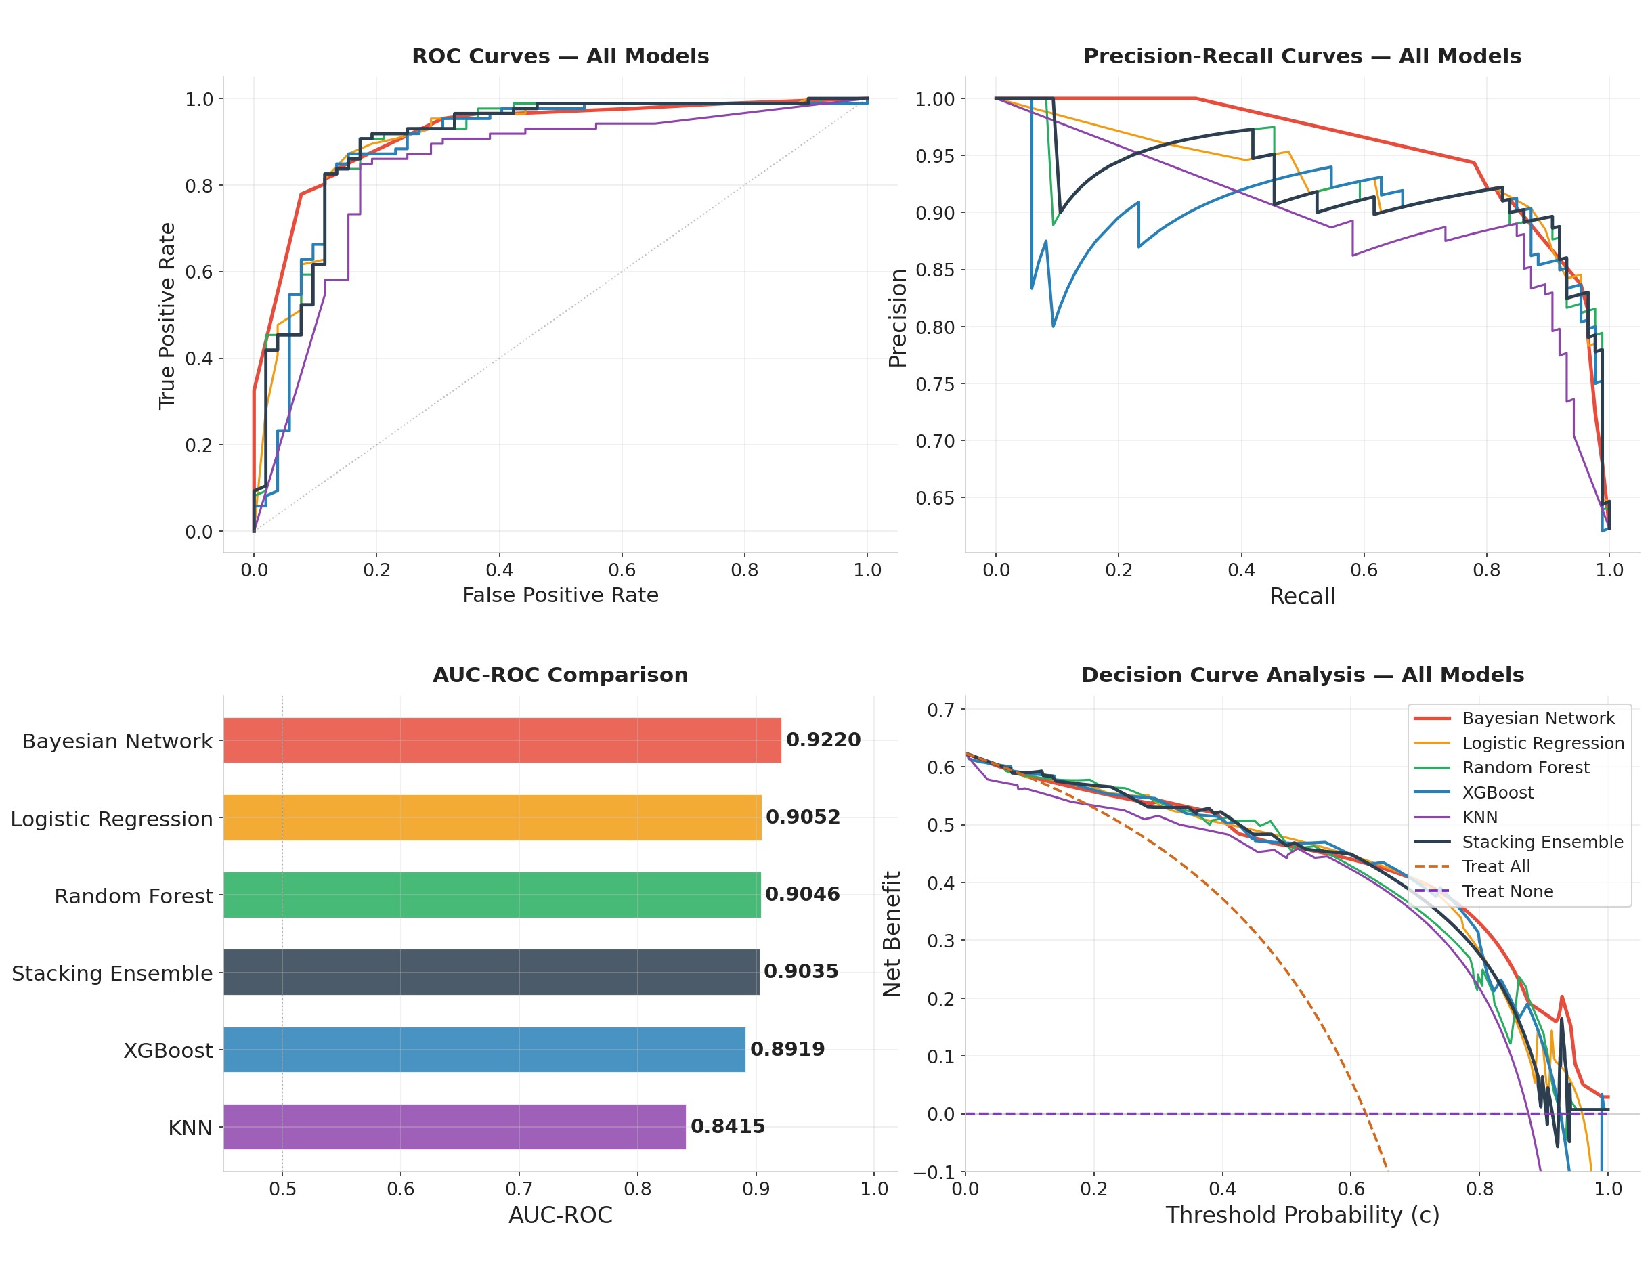
\includegraphics[width=1\textwidth]{image/allmodel/model_au.pdf}
    \caption{So sánh hiệu năng của mô hình mạng Bayes với các mô hình máy học trên bộ dữ liệu Australian Credit}
    \label{fig:auc_au}
\end{figure}
\FloatBarrier

\begin{table}[H]
\centering
\caption{So sánh hiệu năng các mô hình trên Australian Credit}
\label{tab:compare_australian}

\renewcommand{\arraystretch}{1.3}

\begin{tabular}{|p{4cm}|c|c|}
\hline
\rowcolor{gray!20}
\centering\textbf{Mô hình} &
\centering\textbf{ROC-AUC} &
\centering\arraybackslash\textbf{PR-AUC} \\
\hline

Bayesian Network  & 0.9220 & 0.9371 \\
\hline
Logistic Regression & 0.9052 & 0.9218 \\
\hline
Random Forest & 0.9046 & 0.9238 \\
\hline
XGBoost & 0.8919 & 0.8997 \\
\hline
KNN & 0.8415 & 0.8633 \\
\hline
Stacking Ensemble & 0.9055 & 0.9233 \\
\hline

\end{tabular}
\end{table}


\begin{figure}[H]
    \centering
    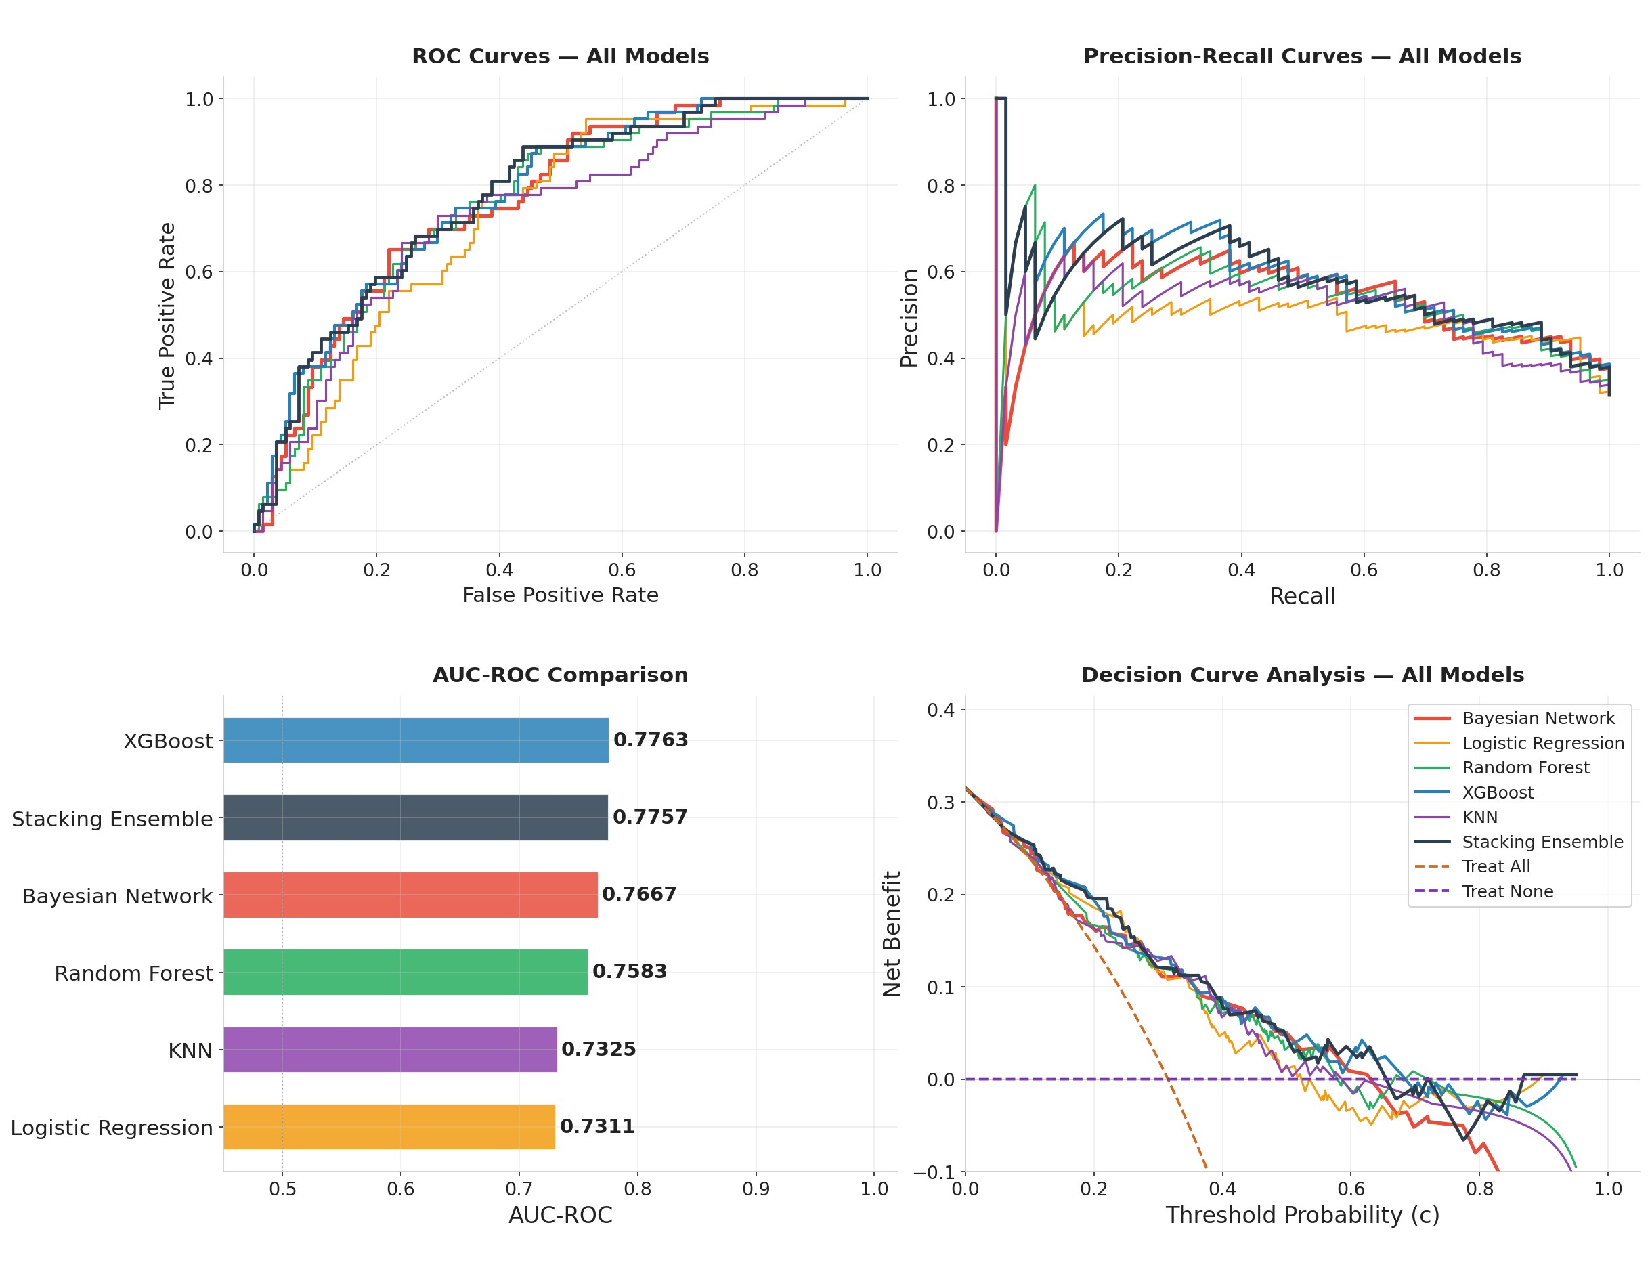
\includegraphics[width=1\textwidth]{image/allmodel/model_ger.pdf}
    \caption{So sánh hiệu năng của mô hình mạng Bayes với các mô hình máy học trên bộ dữ liệu German Credit}
    \label{fig:auc_ger}
\end{figure}


\begin{table}[h]
\centering
\caption{So sánh hiệu năng các mô hình trên German Credit}
\label{tab:compare_german}

\renewcommand{\arraystretch}{1.3}

\begin{tabular}{|p{4cm}|c|c|}
\hline
\rowcolor{gray!20}
\centering\textbf{Mô hình} &
\centering\textbf{ROC-AUC} &
\centering\arraybackslash\textbf{PR-AUC} \\
\hline

Bayesian Network & 0.7667 & 0.5421 \\
\hline
Logistic Regression & 0.7311 & 0.5015 \\
\hline
Random Forest & 0.7583 & 0.5433 \\
\hline
XGBoost & 0.7763 & 0.5888 \\
\hline
KNN & 0.7325 & 0.5172 \\
\hline
Stacking Ensemble & 0.7757 & 0.5785 \\
\hline

\end{tabular}
\end{table}

Trên German Credit (Hình \ref{fig:auc_ger} và Bảng \ref{tab:compare_german}), ROC-AUC = 0.7667 của mạng Bayes vượt trội hơn Logistic Regression, Random Forest và KNN, nhưng thấp hơn nhẹ so với XGBoost (0.7763) và Stacking Ensemble (0.7757).


\begin{figure}[H]
    \centering
    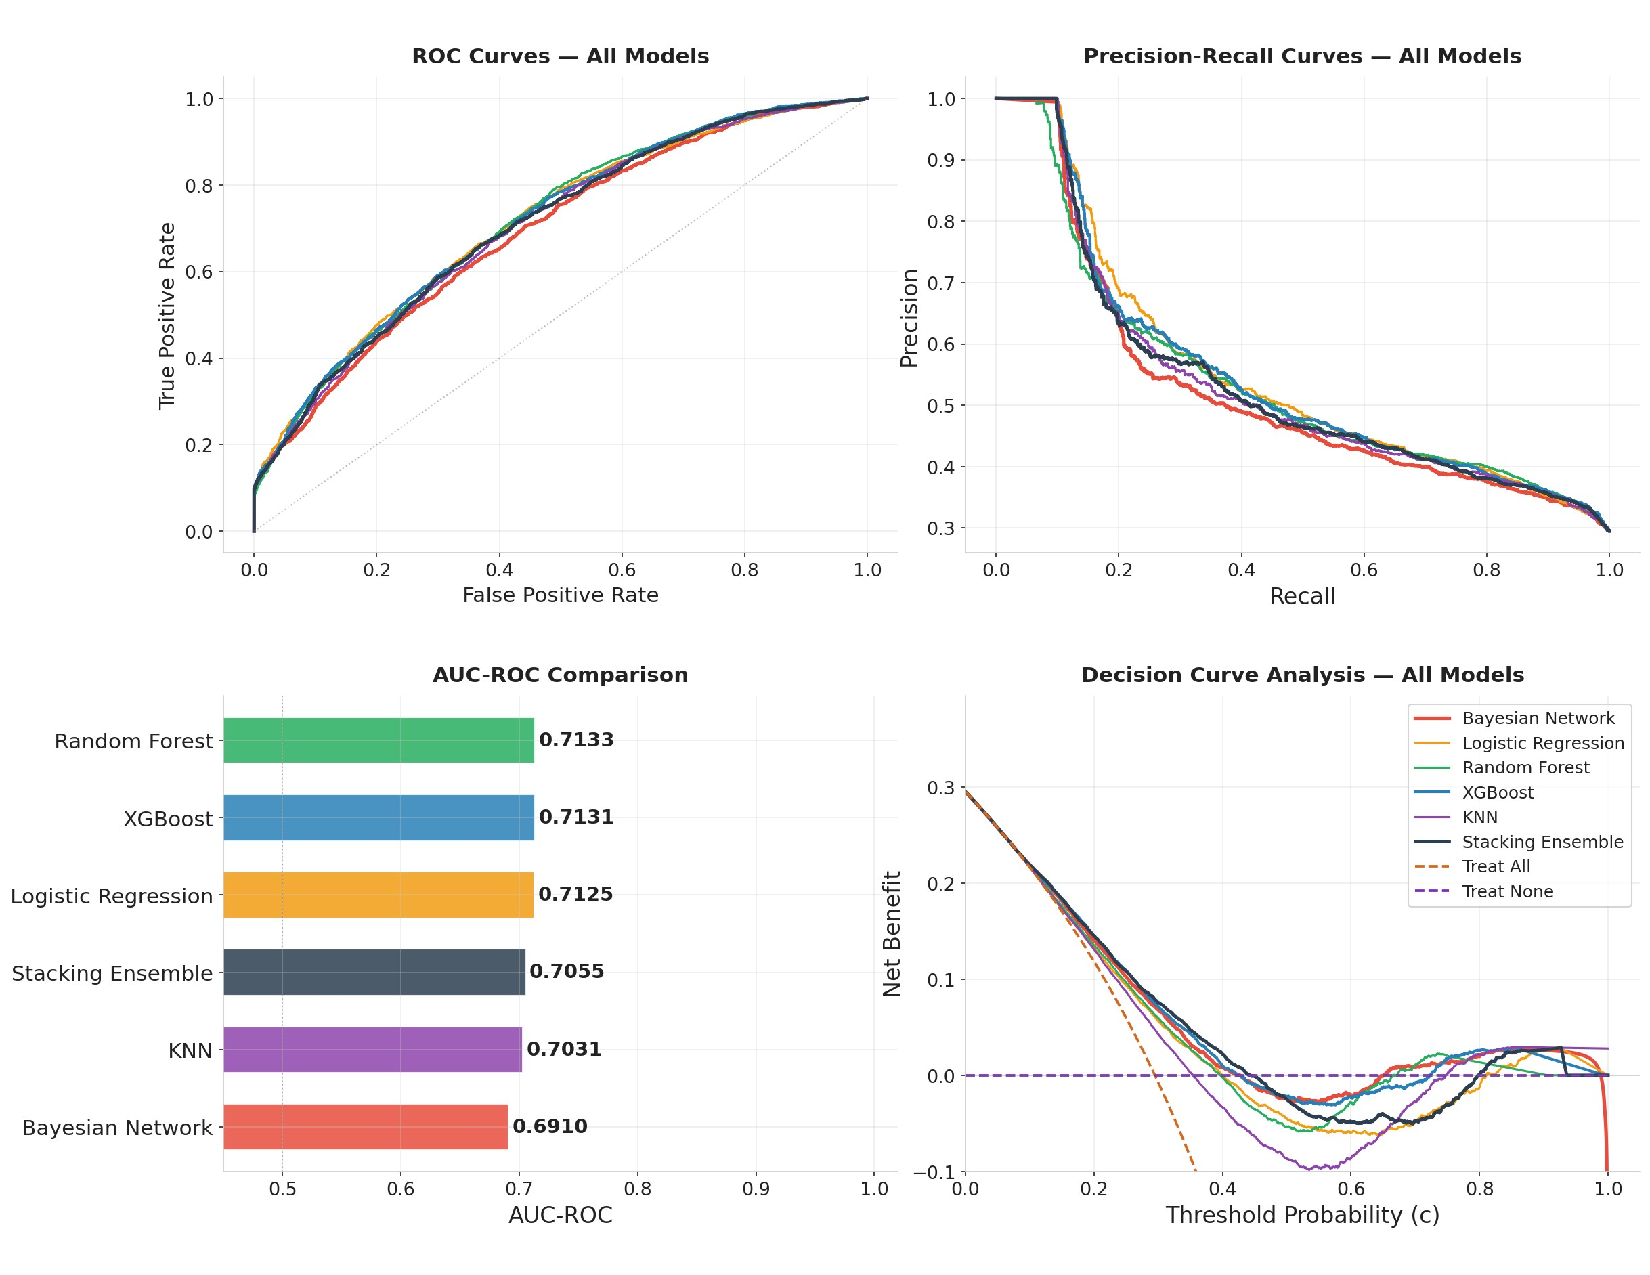
\includegraphics[width=1\textwidth]{image/allmodel/model_lend.pdf}

    \caption{So sánh hiệu năng của mô hình mạng Bayes với các mô hình máy học trên bộ dữ liệu Lending Club}
    \label{fig:auc_lend}
\end{figure}

\begin{table}[h]
\centering
\caption{So sánh hiệu năng các mô hình trên Lending Club}
\label{tab:compare_lending}
\renewcommand{\arraystretch}{1.3}

\begin{tabular}{|p{4cm}|c|c|}
\hline
\rowcolor{gray!20}
\centering\textbf{Mô hình} &
\centering\textbf{ROC-AUC} &
\centering\arraybackslash\textbf{PR-AUC} \\
\hline

Bayesian Network & 0.6910 & 0.5224 \\
\hline
Logistic Regression & 0.7125 & 0.5528 \\
\hline
Random Forest & 0.7133 & 0.5395 \\
\hline
XGBoost & 0.7131 & 0.5483 \\
\hline
KNN & 0.7031 & 0.5352 \\
\hline
Stacking Ensemble & 0.7055 & 0.5371 \\
\hline

\end{tabular}
\end{table}

\FloatBarrier

Ngược lại, trên bộ dữ liệu Lending Club (Hình \ref{fig:auc_lend} và Bảng \ref{tab:compare_lending}) quy mô lớn, BN có ROC-AUC thấp nhất (0.6910) trong số sáu mô hình, đứng sau cả bốn mô hình máy học đơn lẻ và Stacking Ensemble. Sự sụt giảm tương đối này phù hợp với nhận định khi số chiều đặc trưng và độ phức tạp cấu trúc DAG tăng (28 node, 58 cạnh), suy diễn xác suất chính xác của BN gặp khó khăn hơn so với các mô hình boosting/ensemble vốn linh hoạt hơn trong việc nắm bắt tương tác phi tuyến giữa nhiều đặc trưng.

Kết quả so sánh cho thấy một phát hiện thực nghiệm có ý nghĩa quan trọng đối với luận điểm của bài nghiên cứu: vị thế tương đối của mạng Bayes so với các mô hình máy học hiện đại (XGBoost, Random Forest) không cố định mà phụ thuộc mạnh vào đặc điểm dữ liệu. Trên bộ dữ liệu lớn, nhiều đặc trưng và nhiều nhiễu (Lending Club), BN xếp hạng cuối cùng (hạng 6/6), phản ánh hạn chế cố hữu của mạng Bayes rời rạc khi phải xử lý không gian đặc trưng lớn: việc rời rạc hóa biến liên tục gây mất thông tin, và CPT với nhiều tổ hợp trạng thái dễ rơi vào tình trạng ước lượng tham số kém chính xác do dữ liệu thưa trên mỗi ô tổ hợp. Trên German Credit (quy mô trung bình), BN vươn lên hạng 3/6, vượt qua cả Random Forest, KNN và Logistic Regression, chỉ thua Stacking Ensemble và XGBoost với khoảng cách rất nhỏ (dưới 1 điểm phần trăm). Đặc biệt, trên Australian Credit (quy mô nhỏ, ít đặc trưng), BN đạt vị trí dẫn đầu tuyệt đối (hạng 1/6) ở cả hai chỉ số AUC-ROC (0.9220) và AUC-PR (0.9371), vượt qua toàn bộ mô hình đối chứng bao gồm cả Stacking Ensemble, minh chứng rõ ràng cho việc cấu trúc đồ thị xác suất tường minh của BN phát huy lợi thế tối đa khi số lượng biến nhỏ và mối quan hệ nhân quả giữa các biến đơn giản.

\subsection{Suy luận nhân quả (In\_Pro)}
\noindent
Bốn kỹ thuật diễn giải được triển khai tuần tự trên cả ba bộ dữ liệu Australian Credit, German Credit và Lending Club, bao gồm phân tích độ nhạy tham số kết hợp thông tin tương hỗ, suy luận tiến, suy luận lùi kết hợp phân tích kịch bản giả định, và cuối cùng là đối chiếu với hai phương pháp diễn giải hậu kiểm phổ biến là LIME và SHAP. Cách tiếp cận này bám sát khung lý thuyết của Liu và cộng sự \cite{liu2024credit}, theo đó bốn kỹ thuật trên được xem là bốn góc nhìn bổ trợ lẫn nhau để khai thác trọn vẹn khả năng diễn giải nội tại của mạng Bayes, thay vì chỉ dừng lại ở một phép đo đơn lẻ.

\subsubsection{Phân tích độ nhạy}
\label{sec:4.4.1}
\noindent
Áp dụng phương pháp đã trình bày ở Mục \ref{sec: 3.3.3}, nghiên cứu thực nghiệm $\delta$ và thông tin tương hỗ trên cả ba bộ dữ liệu bằng \texttt{pgmpy} và \texttt{scikit-learn}, giới hạn phạm vi khảo sát $\delta$ trong tập biến thuộc Markov Blanket của \texttt{target}.

Đối với Australian Credit, Markov Blanket của \texttt{target} chỉ gồm ba biến \texttt{CreditHistory}, \texttt{Income} và \texttt{Employed}, đúng như cấu trúc đồ thị gọn nhẹ đã ghi nhận tại Mục \ref{sec: 4.3.1}, với $\max|\delta|$ lần lượt là $0.4249$; $0.2871$ và $0.2545$ ở Hình \ref{fig:sens_au}. \texttt{CreditHistory} thể hiện quan hệ đơn điệu rõ ràng tại Hình \ref{fig:prob_au}: khách hàng không có lịch sử tín dụng mang xác suất vỡ nợ $92.5\%$, trong khi khách hàng đã có lịch sử tín dụng giảm mạnh xuống còn $18.3\%$, phản ánh đúng vai trò của biến này như một chỉ báo uy tín nền tảng. Ngược lại, \texttt{Income} không biểu hiện quan hệ đơn điệu qua bốn bin: xác suất vỡ nợ tăng từ $60.1\%$ ở bin thấp nhất lên đỉnh $69.3\%$ ở bin thứ hai, trước khi giảm dần còn $50.2\%$ và $21.3\%$ ở hai bin cao nhất. Hiện tượng phản trực giác này có thể xuất phát từ việc xác suất hậu nghiệm của \texttt{Income} đã được tích hợp qua toàn bộ cấu trúc phụ thuộc với \texttt{CreditHistory} và \texttt{Employed} trong Markov Blanket, khiến một bin thu nhập cụ thể trùng lặp cao với nhóm khách hàng thiếu lịch sử tín dụng hoặc chưa có việc làm ổn định; quy mô mẫu nhỏ của bộ dữ liệu này cũng làm một số bin sau rời rạc hóa dễ bị nhiễu thống kê hơn.

\vspace{1em}
% =========================================================================
% KHỐI HÌNH 4.7 - PHẦN 1: Australian Credit (lấp khoảng trống còn lại)
% =========================================================================
\begin{figure}[H]
    \centering
    \begin{subfigure}[b]{\textwidth}
        \centering
        \begin{minipage}{0.75\textwidth}
            \centering
            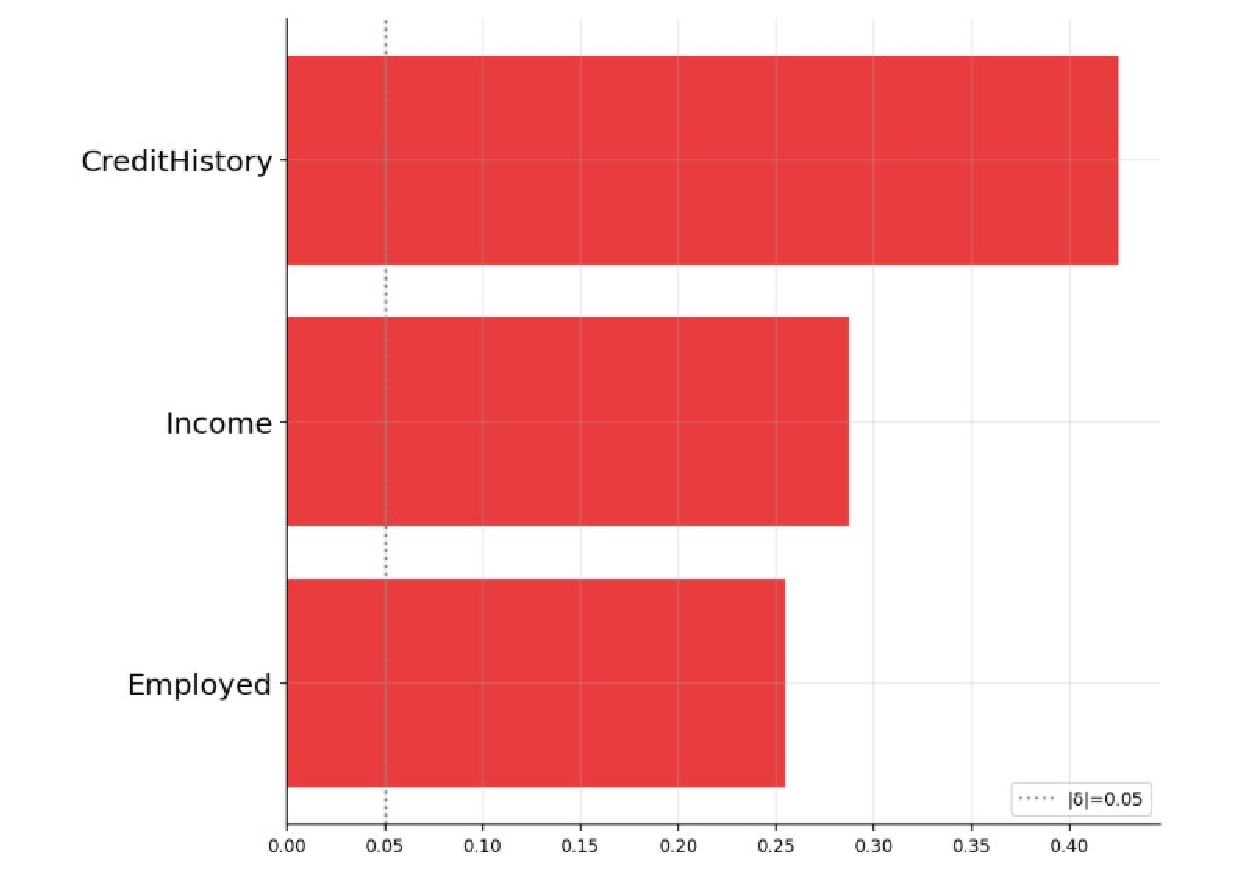
\includegraphics[width=\textwidth]{image/sensitivity/11_sensitivity_au.pdf}\\[0.1cm]
            {\small Biểu đồ độ nhạy ($\delta$)}
        \end{minipage}
        \vspace{0.3cm}
        \begin{minipage}{0.8\textwidth}
            \centering
            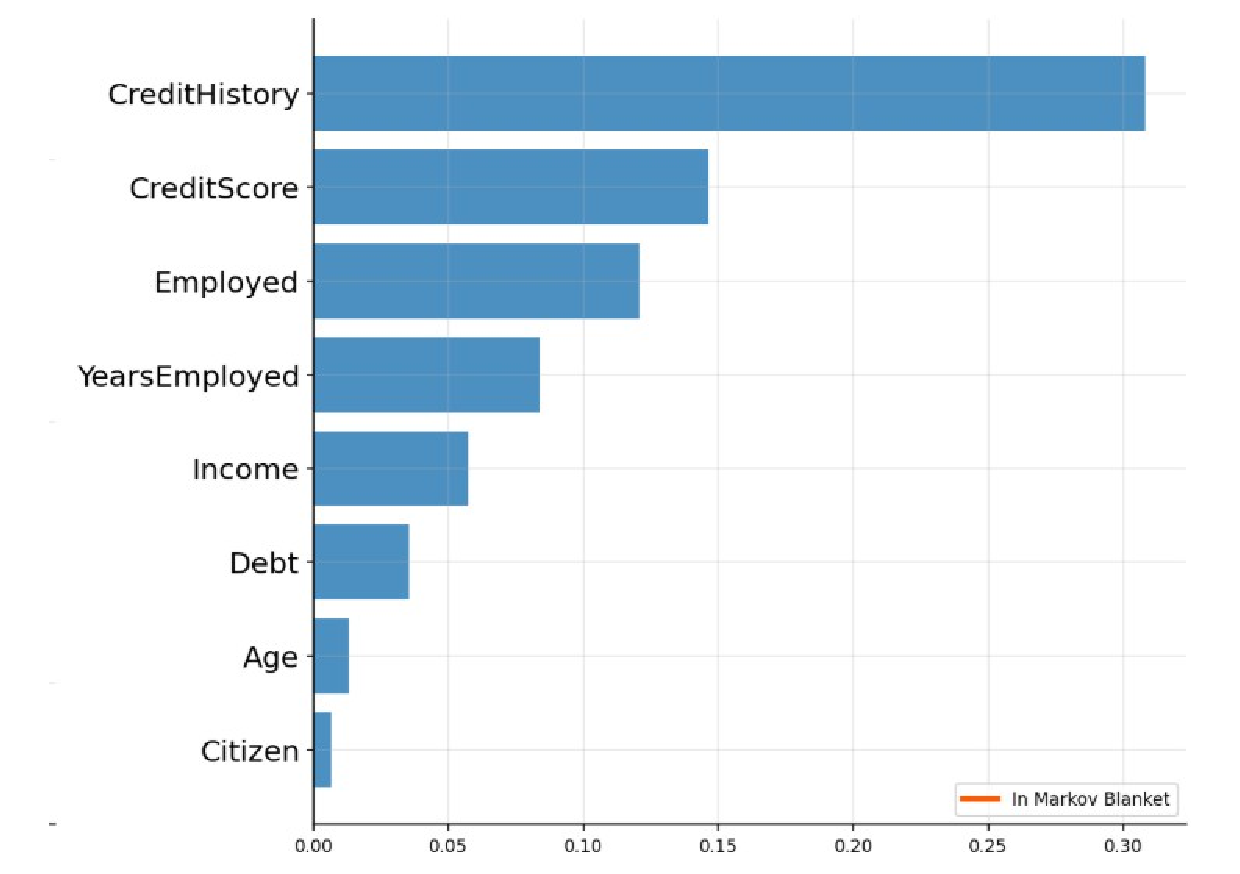
\includegraphics[width=\textwidth]{image/sensitivity/12_sensitivity_au.pdf}\\[0.1cm]
            {\small Thông tin tương hỗ}
        \end{minipage}    
    \end{subfigure}
    \caption{Biểu đồ độ nhạy ($\delta$) và thông tin tương hỗ trên tập biến thuộc Markov Blanket --- Australian Credit}
    \label{fig:sens_au}
\end{figure}
\FloatBarrier

Trên German Credit, Markov Blanket mở rộng lên 11 biến, dẫn đầu về $\delta$ lần lượt là \texttt{job} ($0.4114$), \texttt{purpose} ($0.3667$), \texttt{other\_installment\_plans} ($0.3614$), \texttt{month\_duration} ($0.3600$), \texttt{is\_foreign\_worker} ($0.3592$), \texttt{credit\_history} ($0.3537$), \texttt{secondary\_obligor} ($0.3430$), \texttt{status\_and\_sex} ($0.2882$), \texttt{status\_account} ($0.2115$), \texttt{collateral} ($0.0936$) và \texttt{housing} ($0.0838$) ở Hình \ref{fig:sens_ger}. Đáng chú ý, thứ hạng theo $\delta$ không trùng khớp với thứ hạng theo thông tin tương hỗ: biến có thông tin tương hỗ cao nhất với \texttt{target} là \texttt{secondary\_obligor}, theo sau là \texttt{other\_installment\_plans} và \texttt{purpose}, trong khi \texttt{job} dẫn đầu về $\delta$ chỉ xếp thứ bảy trên trục thông tin tương hỗ, cho thấy hai chỉ số này đang phản ánh hai khía cạnh khác nhau của mối liên hệ giữa biến và \texttt{target} trên cùng một mạng. Xét chi tiết hai biến nhạy nhất tại Hình \ref{fig:prob_ger}, \texttt{is\_foreign\_worker} cho thấy khách hàng là lao động nước ngoài mang xác suất vỡ nợ $85.9\%$, cao hơn đáng kể so với $42.7\%$ của nhóm không phải lao động nước ngoài. \texttt{other\_installment\_plans} lại cho kết quả phi tuyến tương tự \texttt{Income} ở Australian Credit: nhóm có khoản trả góp tại ngân hàng khác mang xác suất $70.8\%$, nhóm có khoản trả góp tại cửa hàng giảm còn $37.8\%$, nhưng nhóm không có bất kỳ khoản trả góp nào khác lại đạt xác suất cao nhất $86.1\%$, nhiều khả năng do trùng lặp với nhóm có \texttt{status\_account} hoặc \texttt{credit\_history} bất lợi trong Markov Blanket, hơn là do bản thân việc không có khoản vay phụ mang ý nghĩa rủi ro độc lập.

Trên Lending Club, Markov Blanket gồm 15 biến, tương ứng với DAG 58 cạnh đã ghi nhận tại Bảng \ref{tab:result_dag}. Ở Hình \ref{fig:sens_lend}, \texttt{debt\_settlement\_flag} và \texttt{num\_accts\_ever\_120\_pd} đạt $\delta = 0.5000$, khả năng phản ánh hiện tượng dữ liệu thưa tương tự trường hợp \texttt{revol\_util} đã ghi nhận ở Mục \ref{sec: 4.2.5}, hơn là một hiệu ứng nhân quả tuyệt đối, và cần được diễn giải thận trọng. Theo sau là \texttt{grade} ($0.3395$), \texttt{int\_rate} ($0.2746$), \texttt{purpose} ($0.2435$), \texttt{fico\_range\_low} ($0.1486$), \texttt{home\_ownership} ($0.1465$) và \texttt{term} ($0.1392$); trong đó \texttt{grade} và \texttt{int\_rate} cũng đồng thời là hai biến dẫn đầu về thông tin tương hỗ trong cùng biểu đồ. Các biến còn lại như \texttt{acc\_open\_past\_24mths}, \texttt{inq\_last\_6mths}, \texttt{loan\_amnt}, \texttt{mths\_since\_recent\_inq}, \texttt{tot\_cur\_bal}, \texttt{num\_actv\_rev\_tl} và \texttt{mort\_acc} đều có $\max|\delta|$ dưới ngưỡng $0.1$, thể hiện mức độ tác động không đáng kể đến xác suất vỡ nợ so với nhóm biến kể trên. Xét chi tiết hai biến dẫn đầu ở Hình \ref{fig:prob_lend}, xác suất vỡ nợ theo \texttt{grade} tăng từ $16.1\%$ ở hạng tín dụng cao nhất lên $67.4\%$ ở hạng gần thấp nhất, sau đó dao động nhẹ quanh $65\%$--$67\%$ ở hai hạng thấp nhất, cho thấy hiệu ứng biên giảm dần khi khách hàng đã rơi vào nhóm rủi ro cao. Đối với \texttt{int\_rate}, xác suất vỡ nợ tăng đơn điệu và gần như tuyến tính từ $22.5\%$ ở bin lãi suất thấp nhất lên $69.1\%$ ở bin cao nhất.

Tổng hợp trên cả ba bộ dữ liệu, các đặc trưng phản ánh trực tiếp lịch sử tín dụng và định giá rủi ro của bên cho vay (\texttt{CreditHistory}, \texttt{credit\_history}, \texttt{grade}, \texttt{int\_rate}) luôn nằm trong nhóm dẫn đầu về mức độ tác động đến xác suất vỡ nợ, phù hợp với trực giác chuyên gia tín dụng truyền thống. Việc đối chiếu $\delta$ với thông tin tương hỗ còn giúp nhận diện các trường hợp mà biên độ dịch chuyển xác suất lớn không đến từ một mối quan hệ nhân quả bền vững mà từ hiện tượng dữ liệu thưa hoặc hiệu ứng nhiễu qua cấu trúc mạng, một khả năng chẩn đoán mà các phương pháp diễn giải hậu kiểm dạng khép kín khó có thể cung cấp trực tiếp.

\begin{figure}[H]
    \centering
    \begin{subfigure}[b]{\textwidth}
        \centering
        \begin{minipage}{0.9\textwidth}
            \centering
            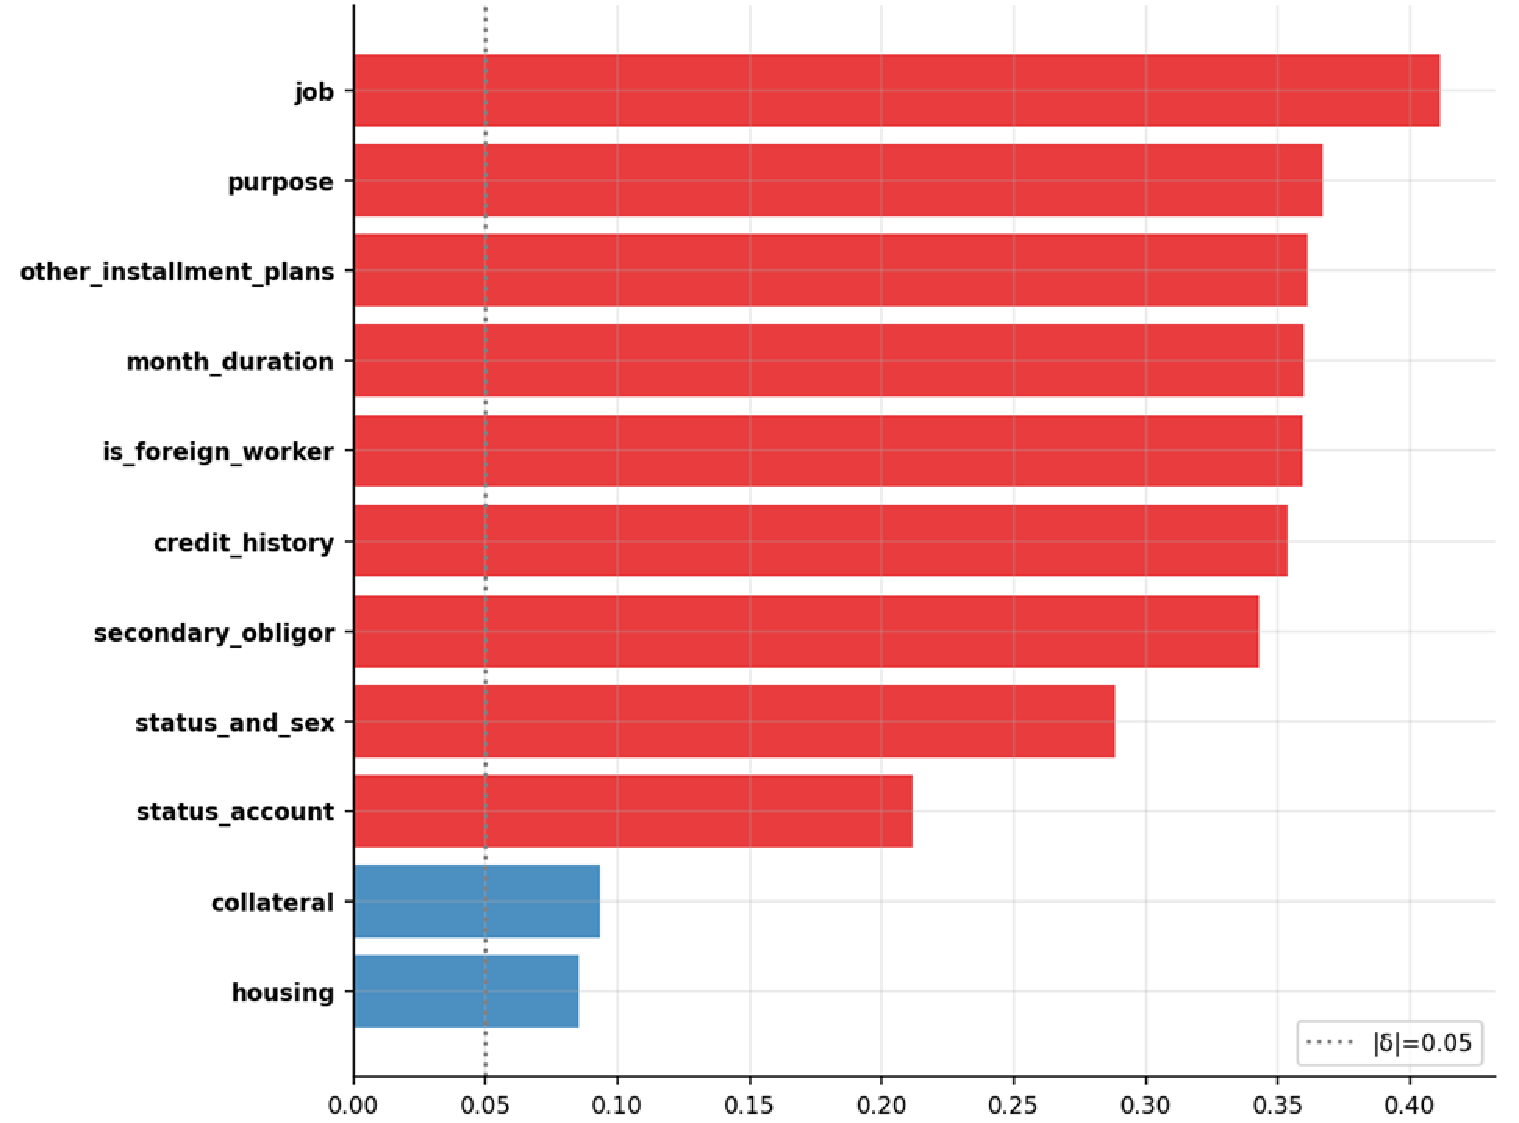
\includegraphics[width=\textwidth]{image/sensitivity/11_sensitivity_ger.pdf}\\[0.1cm]
            {\small Biểu đồ độ nhạy ($\delta$)}
        \end{minipage}
        \vspace{0.3cm}
        \begin{minipage}{0.9\textwidth}
            \centering
            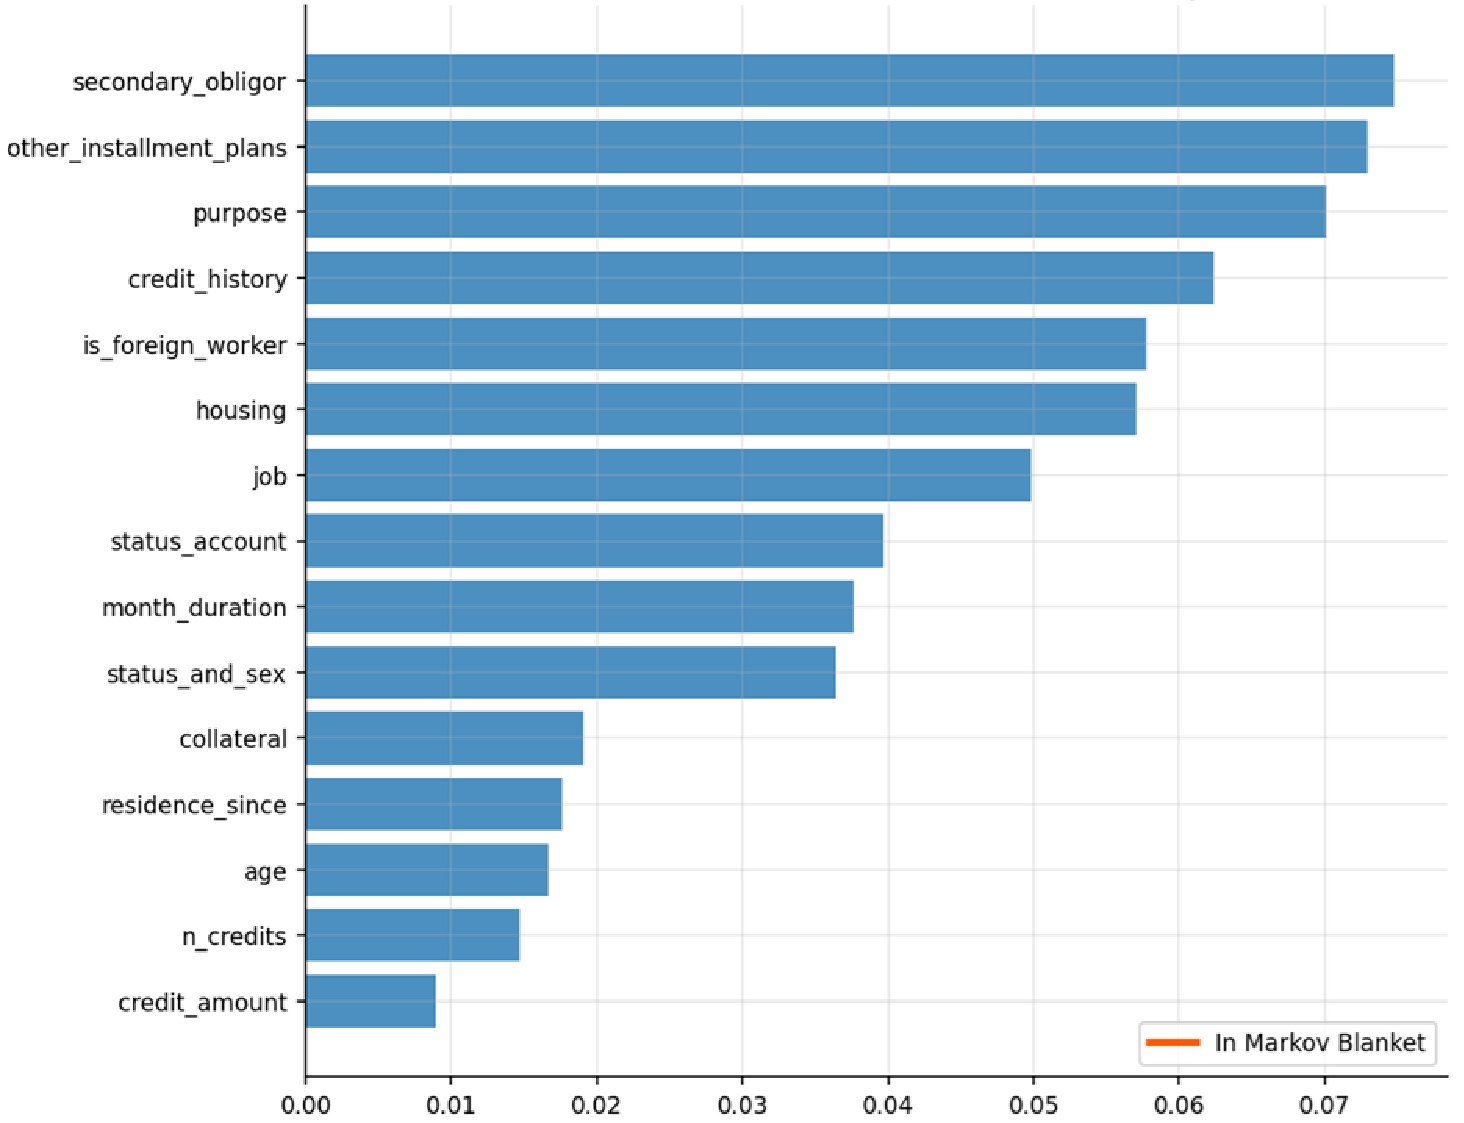
\includegraphics[width=\textwidth]{image/sensitivity/12_sensitivity_ger.pdf}\\[0.1cm]
            {\small Thông tin tương hỗ}
        \end{minipage}    
    \end{subfigure}
    \caption{Biểu đồ độ nhạy ($\delta$) và thông tin tương hỗ trên tập biến thuộc Markov Blanket --- German Credit}
    \label{fig:sens_ger}
\end{figure}

\begin{figure}[H]
    \centering
    \begin{subfigure}[b]{\textwidth}
        \centering
        \begin{minipage}{0.9\textwidth}
            \centering
            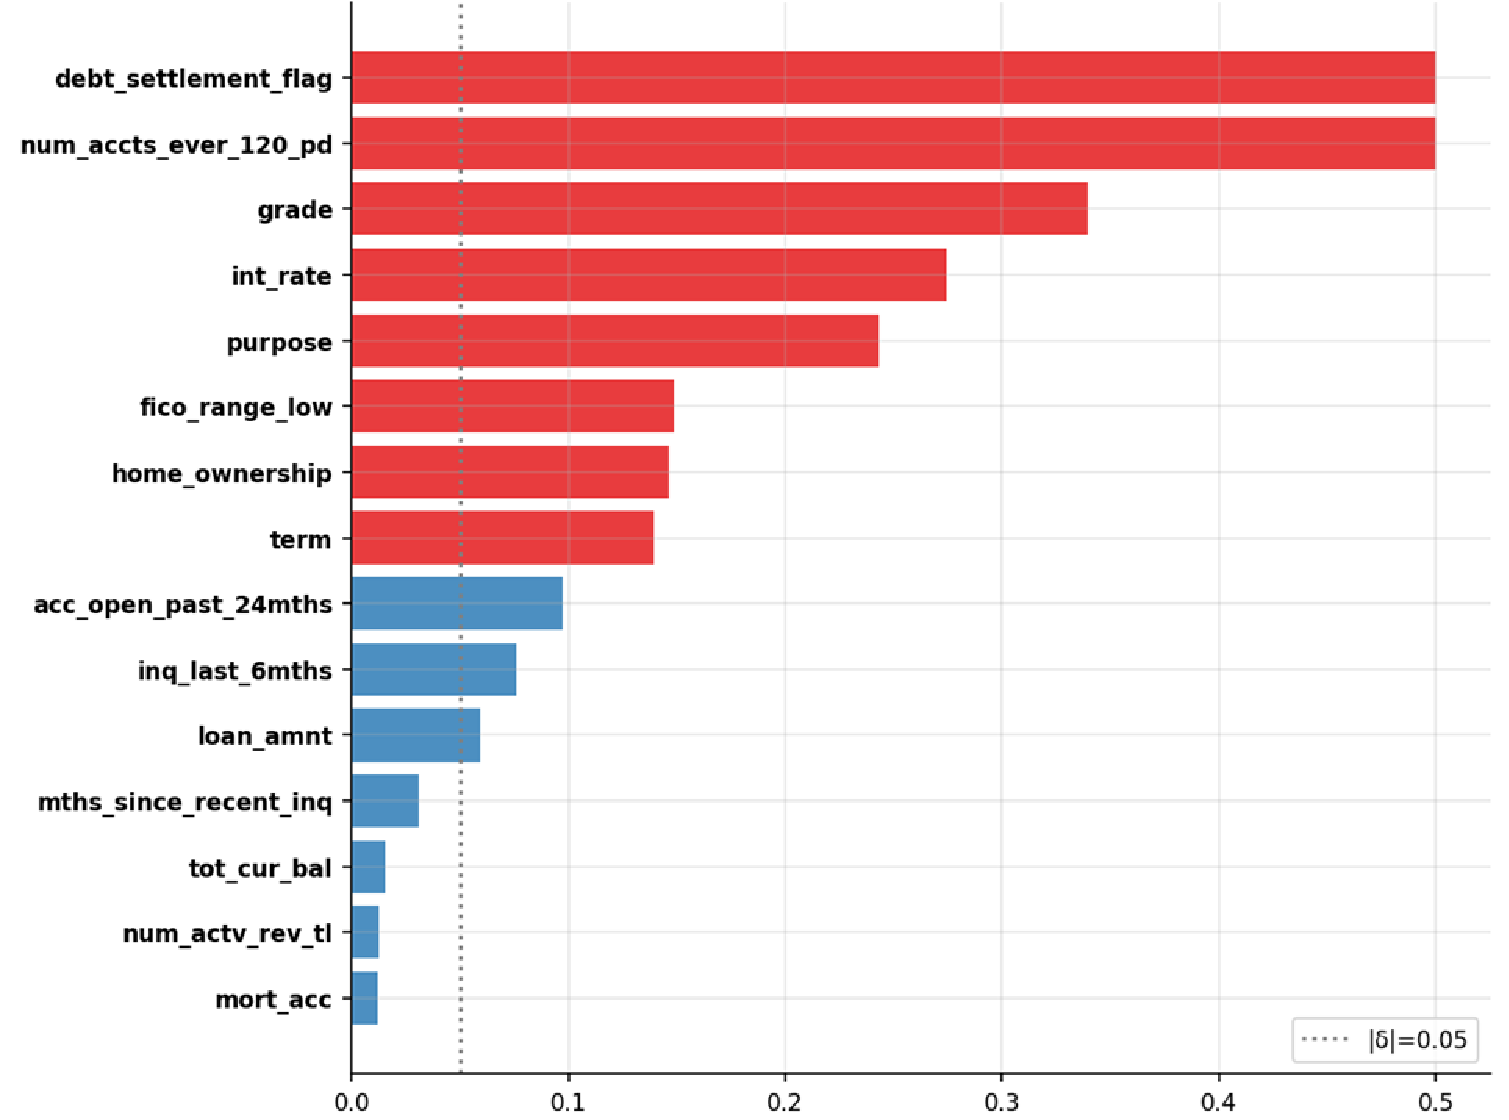
\includegraphics[width=\textwidth]{image/sensitivity/11_sensitivity_lend.pdf}\\[0.1cm]
            {\small Biểu đồ độ nhạy ($\delta$)}
        \end{minipage}
        \vspace{0.3cm}
        \begin{minipage}{0.9\textwidth}
            \centering
            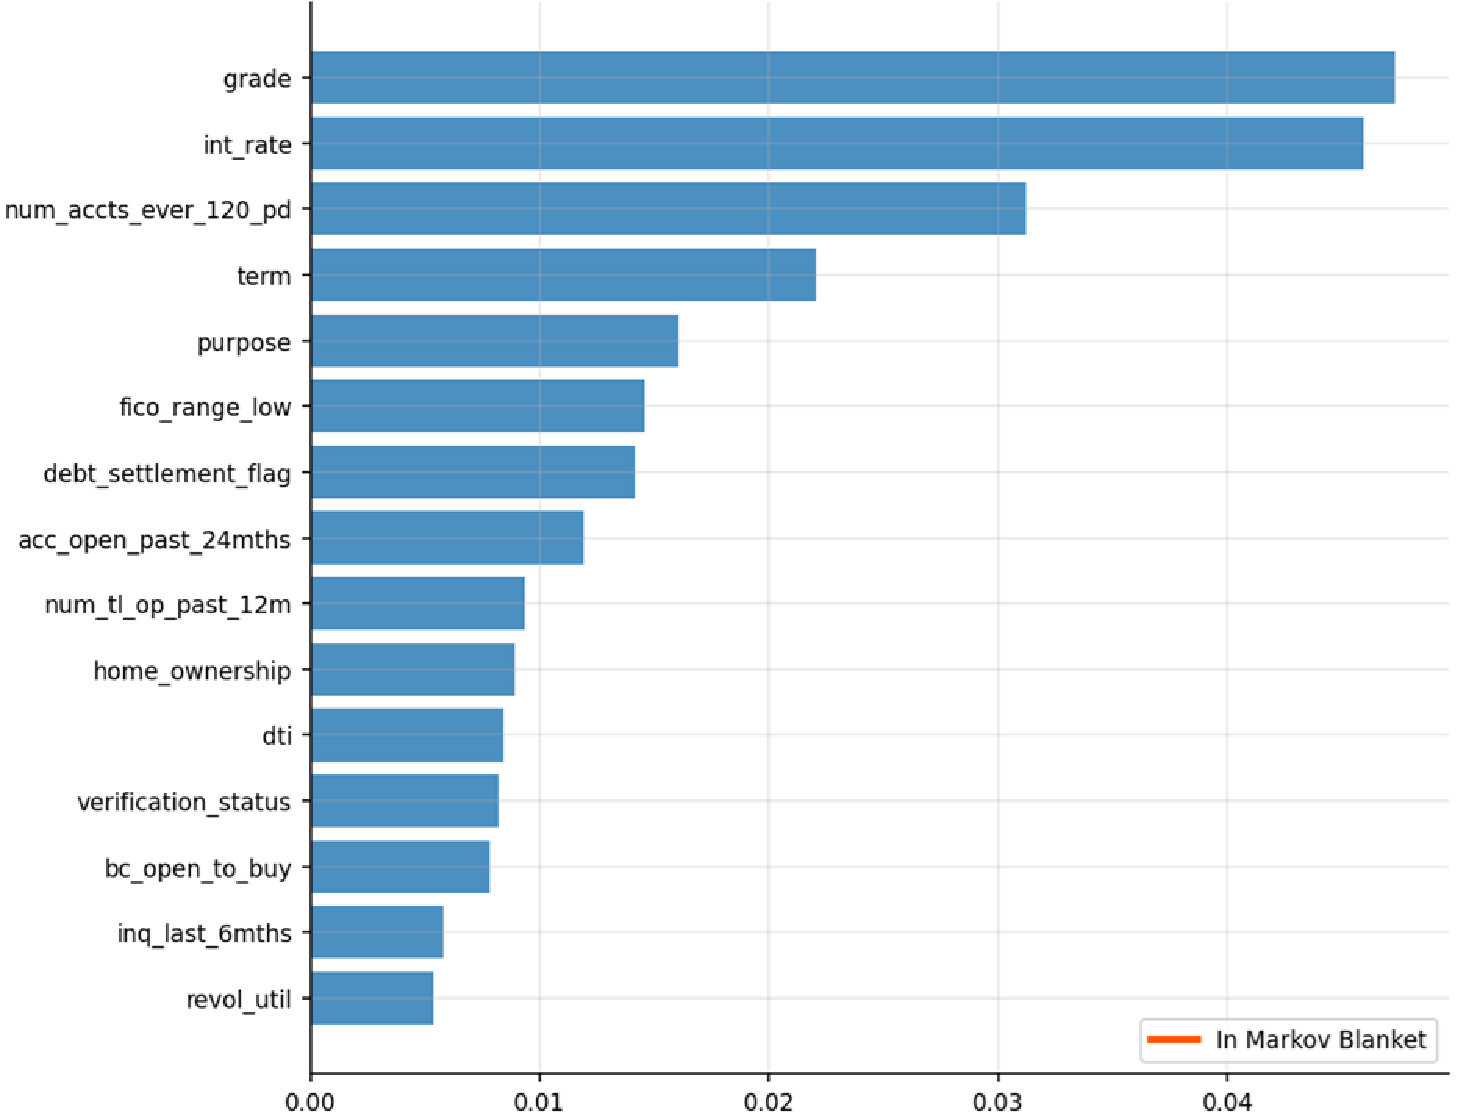
\includegraphics[width=\textwidth]{image/sensitivity/12_sensitivity_lend.pdf}\\[0.1cm]
            {\small Thông tin tương hỗ}
        \end{minipage}    
    \end{subfigure}
    \caption{Biểu đồ độ nhạy ($\delta$) và thông tin tương hỗ trên tập biến thuộc Markov Blanket --- Lending Club}
    \label{fig:sens_lend}
\end{figure}



% =========================================================================
% KHỐI HÌNH 4.8 - PHẦN 1: Australian Credit (lấp khoảng trống còn lại)
% =========================================================================
\begin{figure}[H]
    \centering
    \begin{subfigure}[b]{0.95\textwidth} 
        \centering
        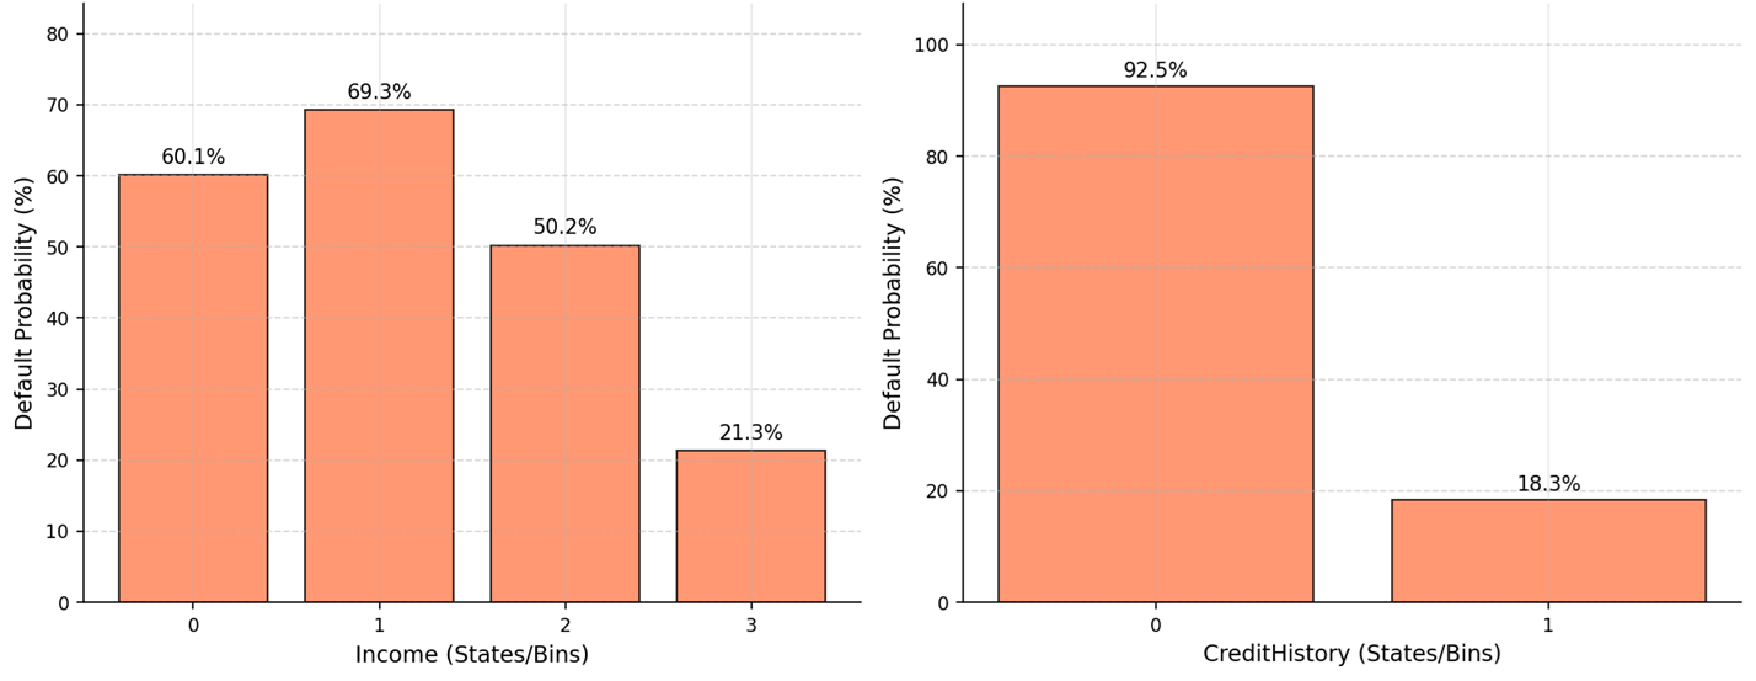
\includegraphics[width=\textwidth]{image/sensitivity/2_sensitivy_au.pdf}       
    \end{subfigure}
    \caption{Xác suất vỡ nợ cận biên khi can thiệp vào các đặc trưng quan trọng --- Australian Credit}
    \label{fig:prob_au}
\end{figure}

\begin{figure}[H]
    \centering
    \begin{subfigure}[b]{0.95\textwidth} 
        \centering
        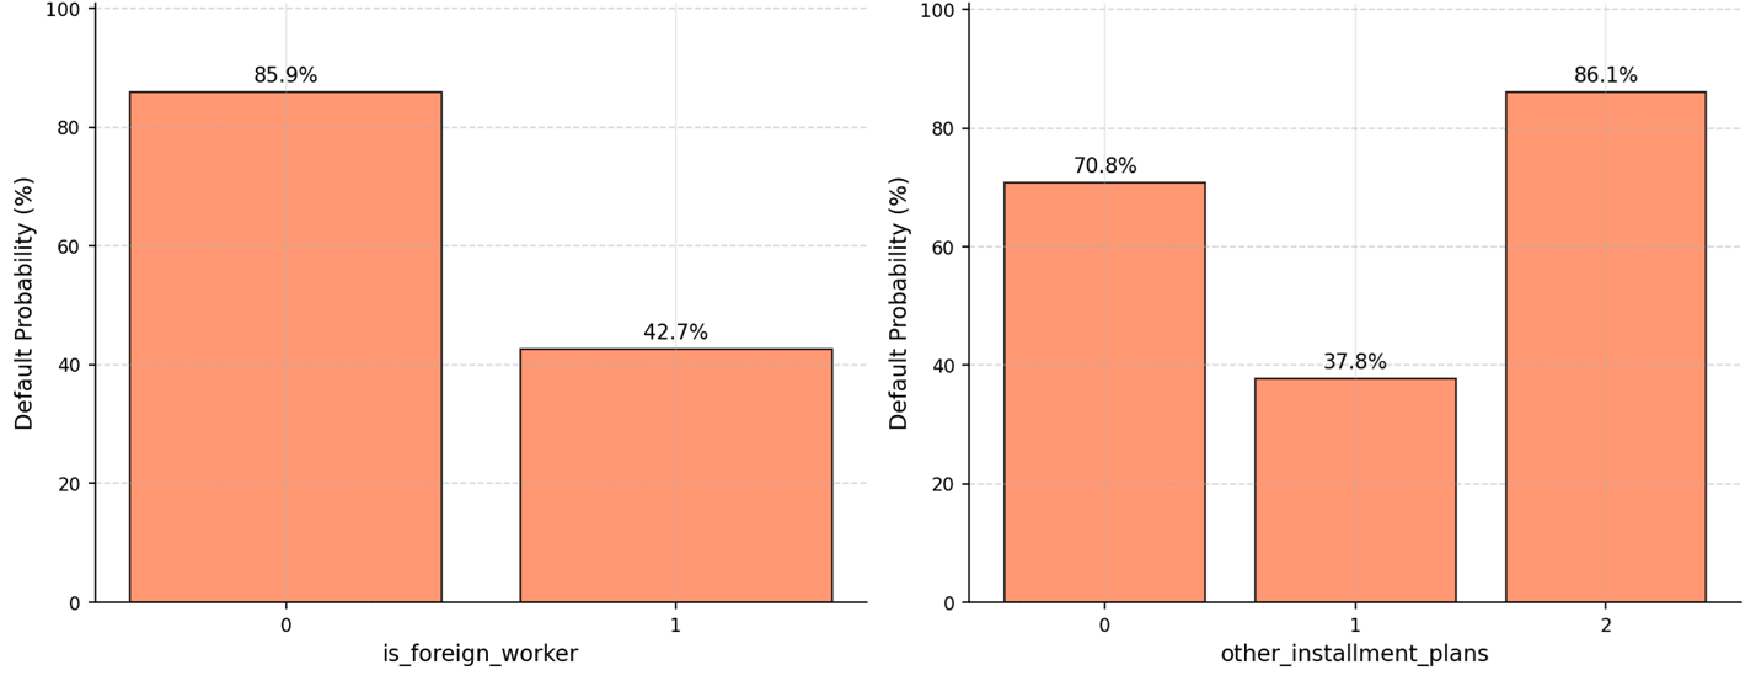
\includegraphics[width=\textwidth]{image/sensitivity/2_sensitivy_ger.pdf}       
    \end{subfigure}
    \caption{Xác suất vỡ nợ cận biên khi can thiệp vào các đặc trưng quan trọng --- German Credit}
    \label{fig:prob_ger}
\end{figure}

\begin{figure}[H]
    \centering
    \begin{subfigure}[b]{1\textwidth} 
        \centering
        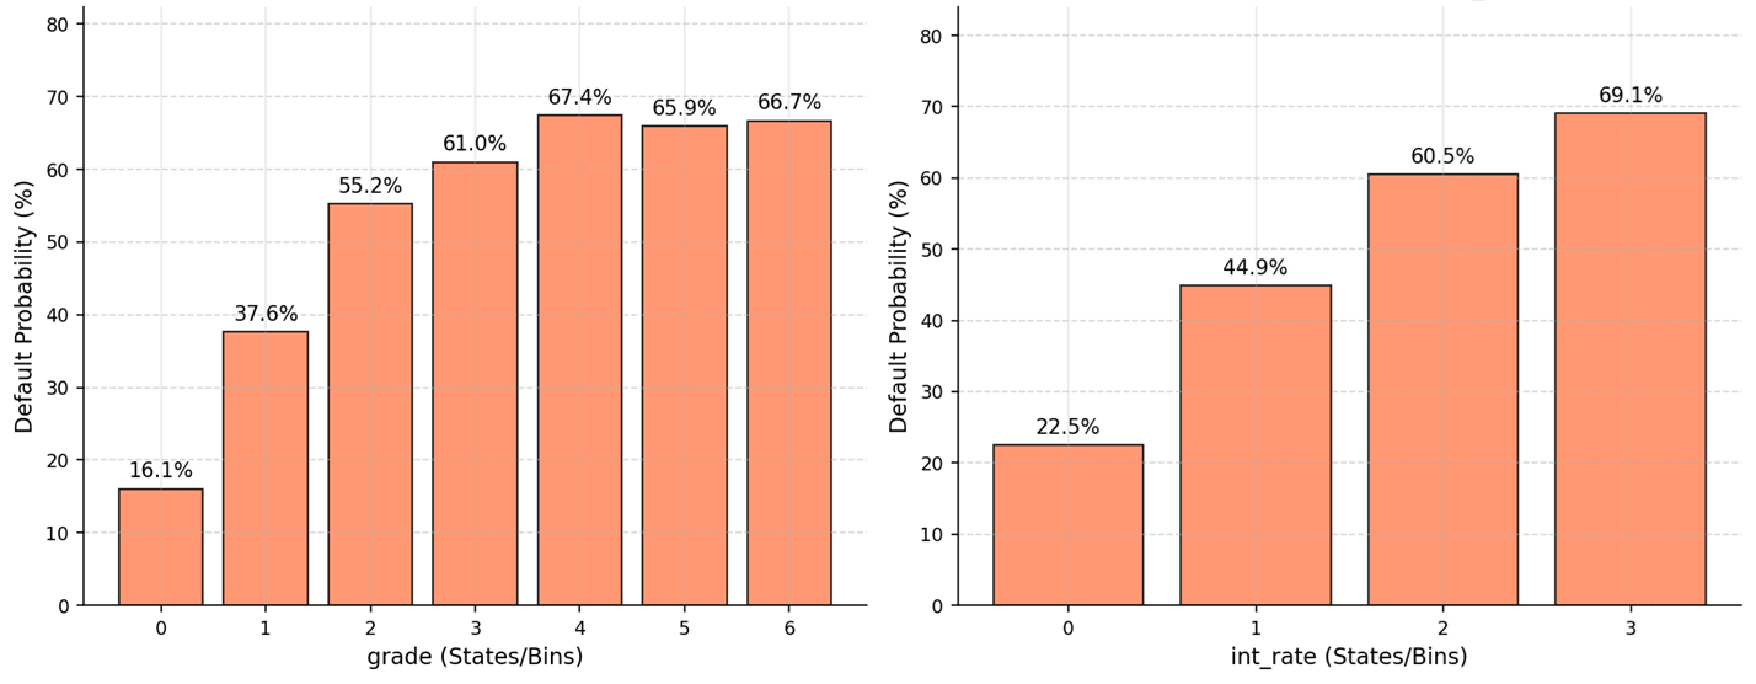
\includegraphics[width=\textwidth]{image/sensitivity/2_sensitivy_lend.pdf}       
    \end{subfigure}
    \caption{Xác suất vỡ nợ cận biên khi can thiệp vào các đặc trưng quan trọng --- Lending Club}
    \label{fig:prob_lend}
\end{figure}

\newpage
\subsubsection{Suy luận tiến}
\label{sec:4.4.2}
\noindent
Suy luận tiến được thực hiện đồng thời trên cặp biến cha (\textit{parent}) trực tiếp của \texttt{target} trong DAG của mỗi bộ dữ liệu, nhằm quan sát hiệu ứng tương tác giữa các nguyên nhân trực tiếp lên xác suất vỡ nợ.

\vspace{1.5em}

% =========================================================================
% KHỐI HÌNH 4.9 - PHẦN 1: Australian Credit (lấp khoảng trống còn lại)
% =========================================================================
\begin{figure}[H]
    \centering
    \begin{subfigure}[b]{0.88\textwidth} 
        \centering
        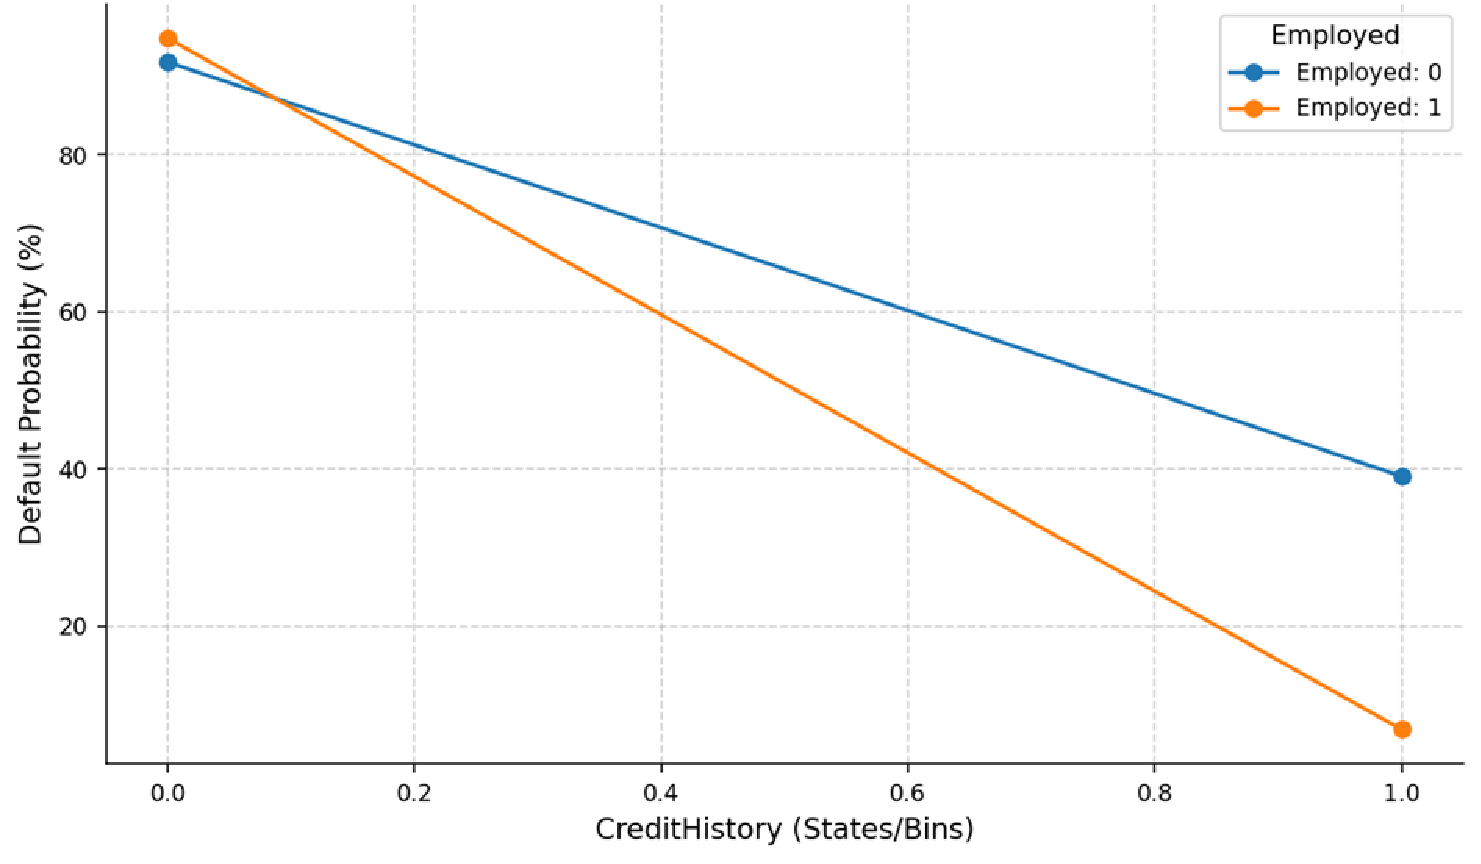
\includegraphics[width=\textwidth]{image/forward/forward_au.pdf}
        \caption{Australian Credit}
        \label{fig:forward_au}
    \end{subfigure}
    
    \vspace{1cm}

    \begin{subfigure}[b]{0.88\textwidth}
        \centering
        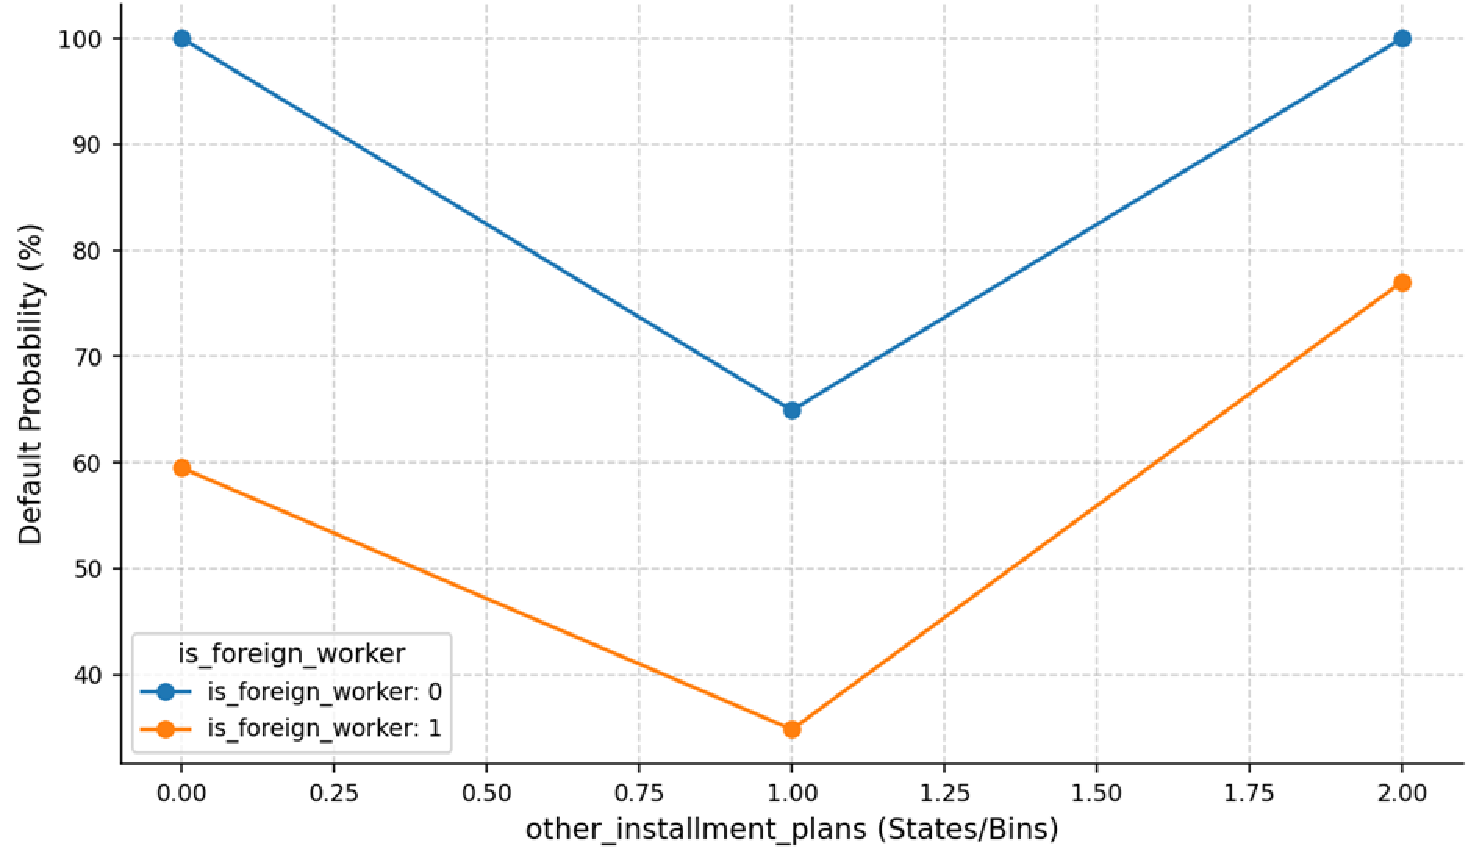
\includegraphics[width=\textwidth]{image/forward/forward_ger.pdf}
        \caption{German Credit}
        \label{fig:forward_ger}
    \end{subfigure}
    
    \caption{Suy luận tiến đồng thời trên cặp biến cha trực tiếp của \texttt{target}}
\end{figure}

% =========================================================================
% KHỐI HÌNH 4.9 - PHẦN 2: German + Lending Club (nối tiếp ngay sau)
% =========================================================================
\begin{figure}[H]
    \ContinuedFloat
    \centering
    
    \begin{subfigure}[b]{0.88\textwidth}
        \centering
        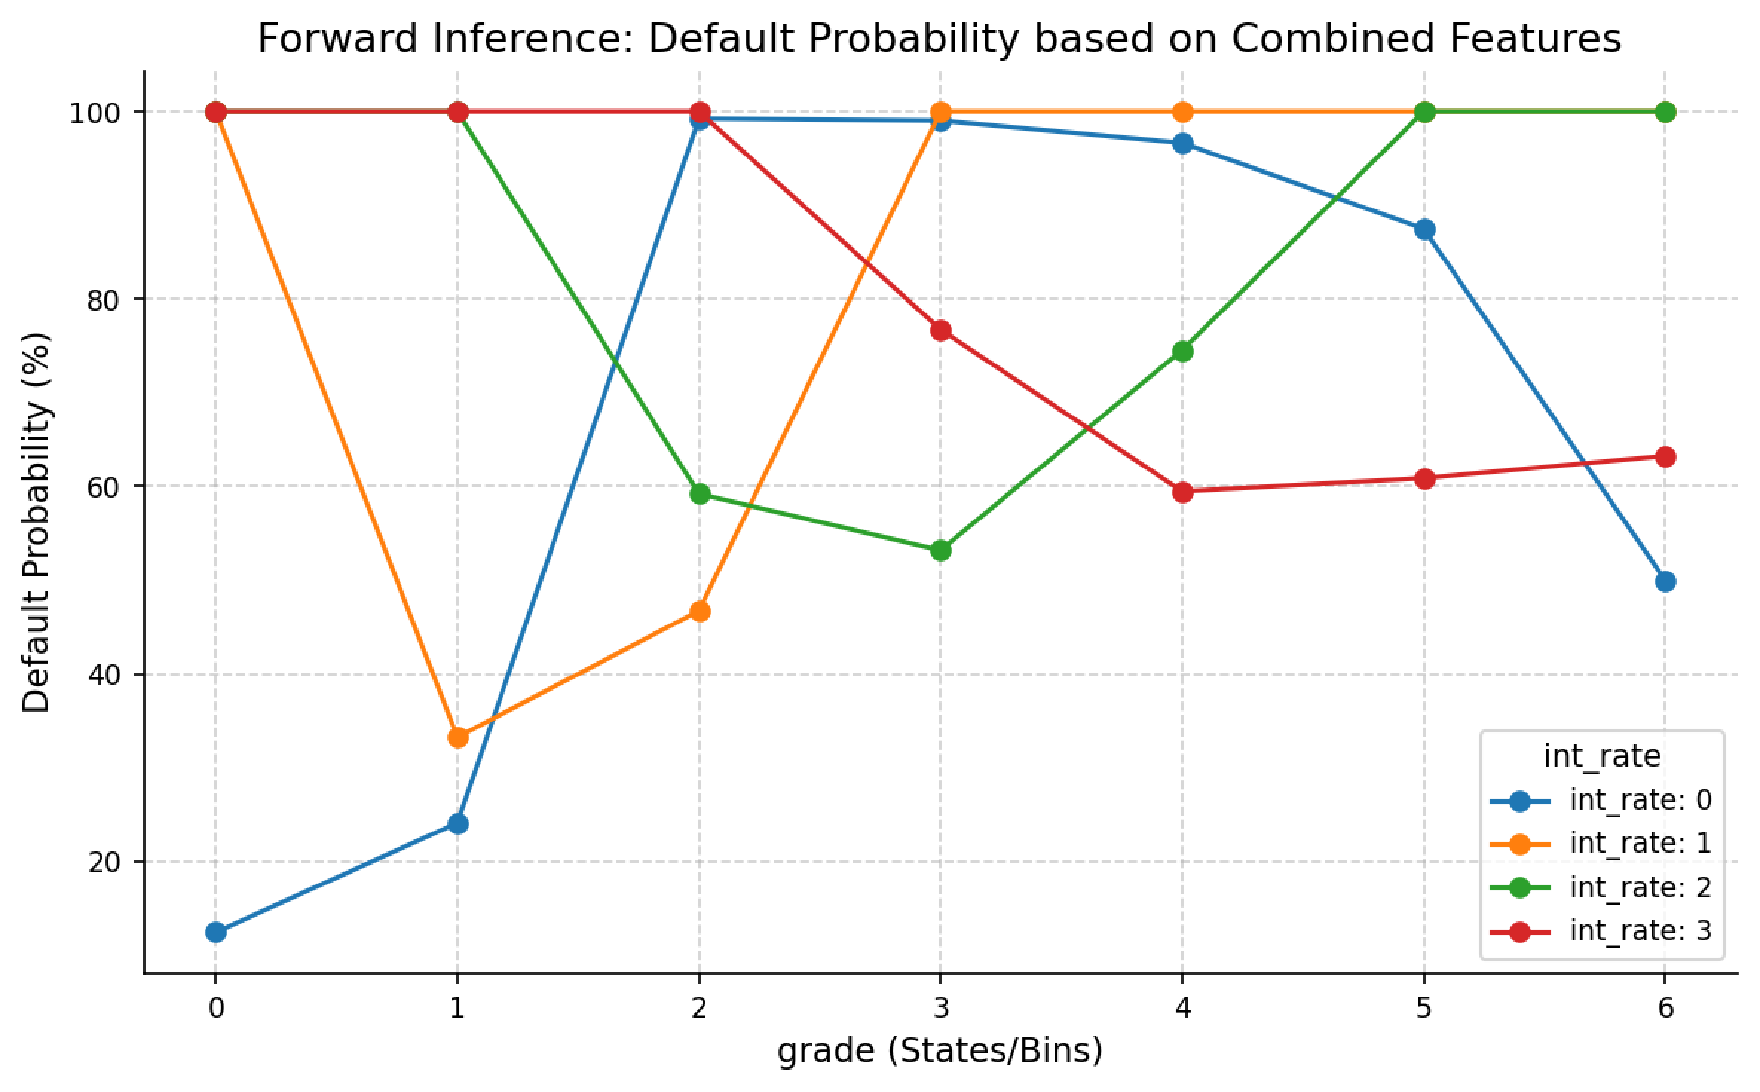
\includegraphics[width=\textwidth]{image/forward/forward_len.pdf}
        \caption{Lending Club}
        \label{fig:forward_len}
    \end{subfigure}
    
    \caption{Suy luận tiến đồng thời trên cặp biến cha trực tiếp của \texttt{target} (tiếp theo)}
    \label{fig:forward_inference}
\end{figure}
\FloatBarrier
Trên Australian Credit, hai biến cha \texttt{CreditHistory} và \texttt{Employed} được gán đồng thời làm bằng chứng. Kết quả tại Hình \ref{fig:forward_au} cho thấy khi khách hàng chưa có lịch sử tín dụng, xác suất vỡ nợ luôn ở mức rất cao bất kể tình trạng việc làm, dao động quanh $93\%$ đối với người chưa có việc làm và tăng nhẹ lên khoảng $95\%$ đối với người đang có việc làm. Khi đã có lịch sử tín dụng, xác suất vỡ nợ giảm mạnh ở cả hai nhóm, nhưng mức giảm rõ rệt hơn hẳn ở nhóm đang có việc làm, chỉ còn khoảng $7\%$, so với khoảng $39\%$ ở nhóm chưa có việc làm. Nói cách khác, \texttt{Employed} không thể hiện vai trò bảo vệ đáng kể khi \texttt{CreditHistory} ở trạng thái bất lợi, nhưng lại khuếch đại rõ rệt hiệu ứng tích cực của \texttt{CreditHistory} khi biến này ở trạng thái thuận lợi.

Trên German Credit, hai biến cha \texttt{is\_foreign\_worker} và \texttt{other\_installment\_plans} được khảo sát đồng thời. Hình \ref{fig:forward_ger} cho thấy cả hai đường ứng với \texttt{is\_foreign\_worker} đều giữ nguyên hình dạng chữ V đã ghi nhận ở \ref{sec:4.4.1} đối với \texttt{other\_installment\_plans}, nhưng bị dịch chuyển theo hai biên độ khác nhau: nhóm lao động nước ngoài đạt xác suất vỡ nợ tối đa $100\%$ ở cả hai trạng thái ``Bank'' và ``none'', trong khi nhóm không phải lao động nước ngoài dù cùng biểu hiện chữ V nhưng đáy và đỉnh đều thấp hơn đáng kể, chỉ dao động trong khoảng $35\%$--$77\%$. Kết quả này cho thấy \texttt{is\_foreign\_worker} đóng vai trò như một biến khuếch đại làm trầm trọng thêm hiệu ứng phi tuyến vốn đã tồn tại của \texttt{other\_installment\_plans}.

Trên Lending Club, hai biến cha \texttt{grade} và \texttt{int\_rate} được khảo sát đồng thời. Khác hẳn với hai bộ dữ liệu trên, Hình \ref{fig:forward_len} cho thấy quan hệ giữa hai biến này không còn đơn điệu hay có quy luật rõ ràng, mà dao động thất thường: ở \texttt{grade} thấp nhất (hạng A, state 0), xác suất vỡ nợ chỉ đạt $13\%$ ở \texttt{int\_rate} thấp nhất nhưng lại nhảy vọt lên gần $100\%$ ở cả ba mức \texttt{int\_rate} còn lại; trong khi đó, ở \texttt{grade} cao nhất (hạng G, state 6), xu hướng gần như đảo ngược khi \texttt{int\_rate} thấp nhất lại cho xác suất vỡ nợ cao nhất trong nhóm ($50\%$) còn ba mức \texttt{int\_rate} còn lại đều xấp xỉ $60\%$--$100\%$. Hiện tượng dao động phi quy luật này nhiều khả năng bắt nguồn từ mối tương quan rất cao giữa \texttt{grade} và \texttt{int\_rate} trong thực tế cho vay của Lending Club, vốn dĩ lãi suất được ấn định phần lớn dựa trên hạng tín dụng ngay từ khâu thẩm định; hệ quả là nhiều tổ hợp (\texttt{grade}, \texttt{int\_rate}) hiếm gặp hoặc gần như không tồn tại trong tập huấn luyện, khiến bảng CPT tương ứng được ước lượng trên rất ít quan sát và cho ra xác suất cực trị kém ổn định, tương tự hiện tượng dữ liệu thưa đã ghi nhận ở Mục \ref{sec:4.4.1} đối với \texttt{debt\_settlement\_flag} và \texttt{num\_accts\_ever\_120\_pd}. Kết quả này là một minh chứng rõ ràng cho giới hạn của việc suy luận đồng thời trên hai biến có tương quan nội tại cao, và cần được diễn giải hết sức thận trọng thay vì rút ra kết luận nhân quả trực tiếp.

Nhìn chung, suy luận tiến trên cặp biến cha đồng thời cho thấy mức độ tương tác giữa các đặc trưng không đồng nhất: Australian Credit và German Credit thể hiện tương tác khuếch đại có quy luật rõ ràng, trong khi Lending Club lại bộc lộ giới hạn của phương pháp khi hai biến cha được chọn có tương quan nội tại quá cao, dẫn đến hiện tượng dữ liệu thưa trong không gian tổ hợp. Phát hiện này khẳng định giá trị bổ sung của suy luận tiến đa biến so với phân tích độ nhạy đơn biến, đồng thời cũng cho thấy việc lựa chọn cặp biến cha để suy luận đồng thời cần cân nhắc thêm yếu tố tương quan nội tại giữa chúng, chứ không chỉ dựa vào quan hệ nhân quả trực tiếp với \texttt{target}.

\subsubsection{Suy luận lùi}
\noindent
Suy luận lùi được thực hiện trên từng biến cha trực tiếp của \texttt{target} trong DAG của mỗi bộ dữ liệu, truy vấn $P(X_i \mid \text{target}=1)$ so với $P(X_i \mid \text{target}=0)$ nhằm truy vết đặc điểm chung của nhóm hồ sơ đã vỡ nợ so với nhóm không vỡ nợ.

Trên Australian Credit, \texttt{CreditHistory} và \texttt{Employed} là hai biến cha được truy vấn. Kết quả tại Hình \ref{fig:backward_au} cho thấy trong nhóm khách hàng đã vỡ nợ, $79.1\%$ không có lịch sử tín dụng, trong khi tỷ lệ này ở nhóm không vỡ nợ chỉ là $6.5\%$, mức chênh lệch lớn nhất trong toàn bộ kết quả \textit{backward inference} của cả ba bộ dữ liệu, khẳng định \texttt{CreditHistory} là dấu hiệu chẩn đoán mạnh nhất để truy vết một hồ sơ đã vỡ nợ. Tương tự, $77.4\%$ nhóm vỡ nợ chưa có việc làm tại thời điểm nộp đơn, so với $30.3\%$ ở nhóm không vỡ nợ, thấp hơn đáng kể so với chênh lệch của \texttt{CreditHistory} nhưng vẫn thể hiện khả năng phân biệt rõ ràng.

Trên German Credit, \texttt{is\_foreign\_worker} và \texttt{other\_installment\_plans} là hai biến cha được truy vấn tại Hình \ref{fig:backward_ger}. Đối với \texttt{is\_foreign\_worker}, $29.19\%$ nhóm vỡ nợ là lao động nước ngoài so với chỉ $4.78\%$ ở nhóm không vỡ nợ, mức chênh lệch cao thứ nhì trong toàn bộ kết quả \textit{backward inference} của ba bộ dữ liệu, chỉ sau \texttt{CreditHistory} của Australian Credit. Đối với \texttt{other\_installment\_plans}, trạng thái ``none'' chiếm $20.81\%$ trong nhóm vỡ nợ so với chỉ $3.35\%$ ở nhóm không vỡ nợ, trong khi trạng thái ``stores'' lại phổ biến hơn hẳn ở nhóm không vỡ nợ ($85.41\%$) so với nhóm vỡ nợ ($51.91\%$). Kết quả này cho thấy chiều phân biệt của \texttt{other\_installment\_plans} không tập trung ở một trạng thái duy nhất mà trải đều ở hai đầu ``Bank'' và ``none'', nhất quán với hình dạng chữ V phi tuyến đã ghi nhận ở Mục \ref{sec:4.4.1} và \ref{sec:4.4.2}.


% =========================================================================
% KHỐI HÌNH 4.10 - PHẦN 1: Australian Credit (lấp khoảng trống còn lại)
% =========================================================================
\begin{figure}[H]
    \centering
    \begin{subfigure}[b]{\textwidth}
        \centering
        \begin{minipage}{0.49\textwidth}
            \centering
            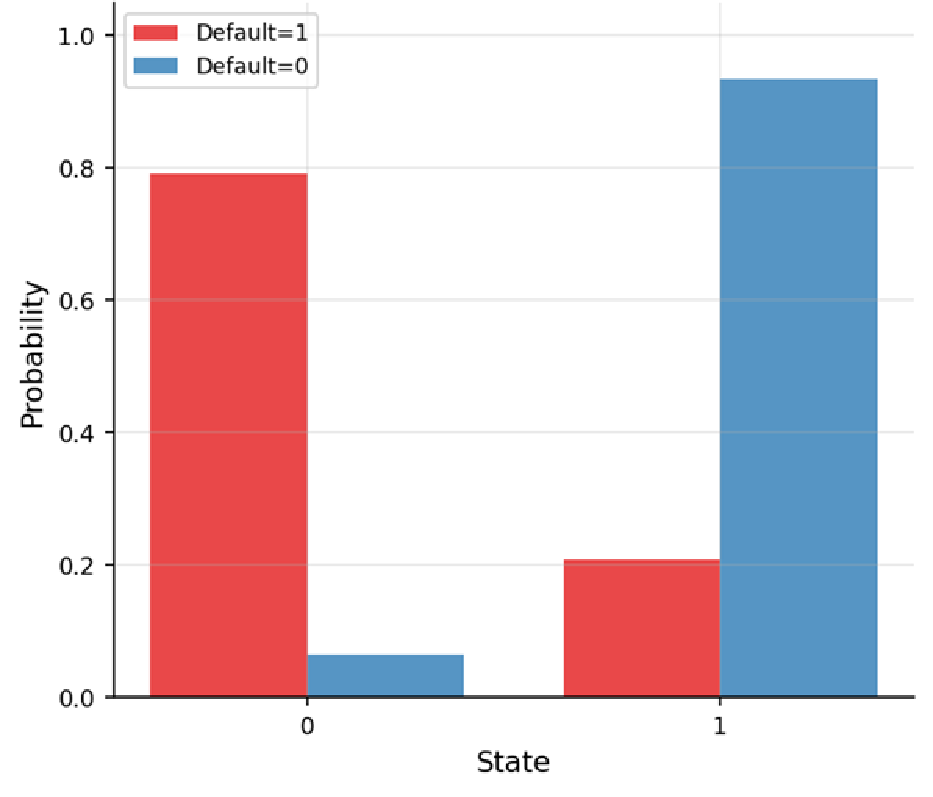
\includegraphics[width=\textwidth]{image/backward/backward_au_crehis.pdf}\\[0.1cm]
            \caption{\texttt{CreditHistory}}
        \end{minipage}
        \hfill
        \begin{minipage}{0.49\textwidth}
            \centering
            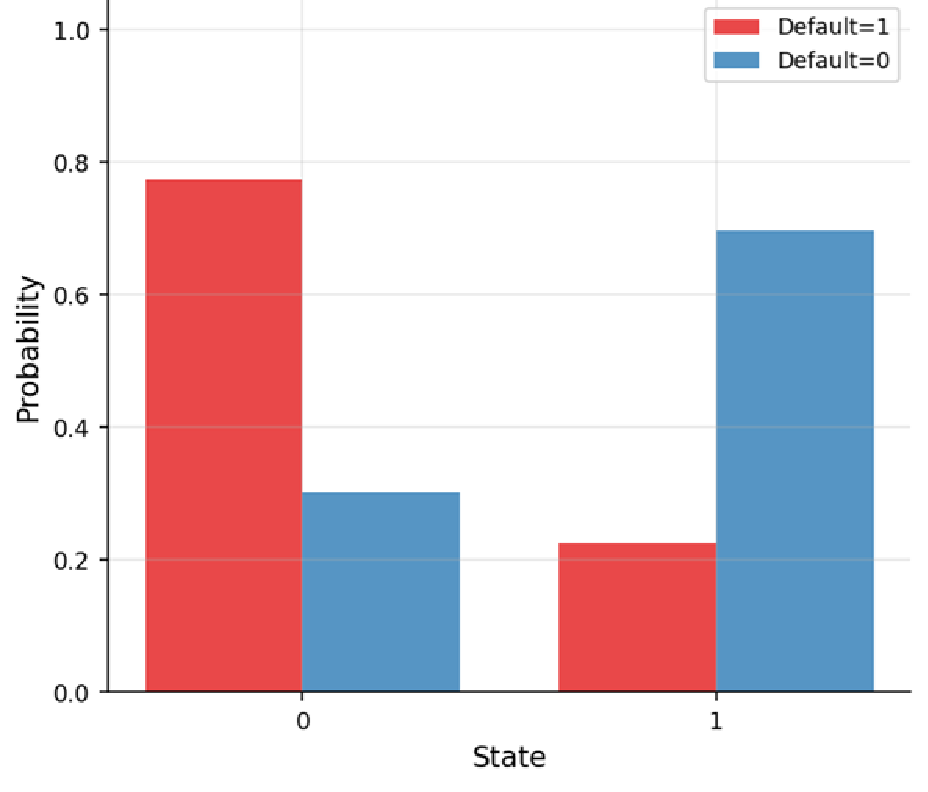
\includegraphics[width=\textwidth]{image/backward/backward_au_employ.pdf}\\[0.1cm]
            \caption{\texttt{Employed}}
        \end{minipage}
    \end{subfigure}
    \caption{Suy luận lùi trên các biến cha trực tiếp của \texttt{target} --- Australian Credit}
    \label{fig:backward_au}
\end{figure}

\begin{figure}[H]
    \centering
    \begin{subfigure}[b]{\textwidth}
        \centering
        \begin{minipage}{0.49\textwidth}
            \centering
            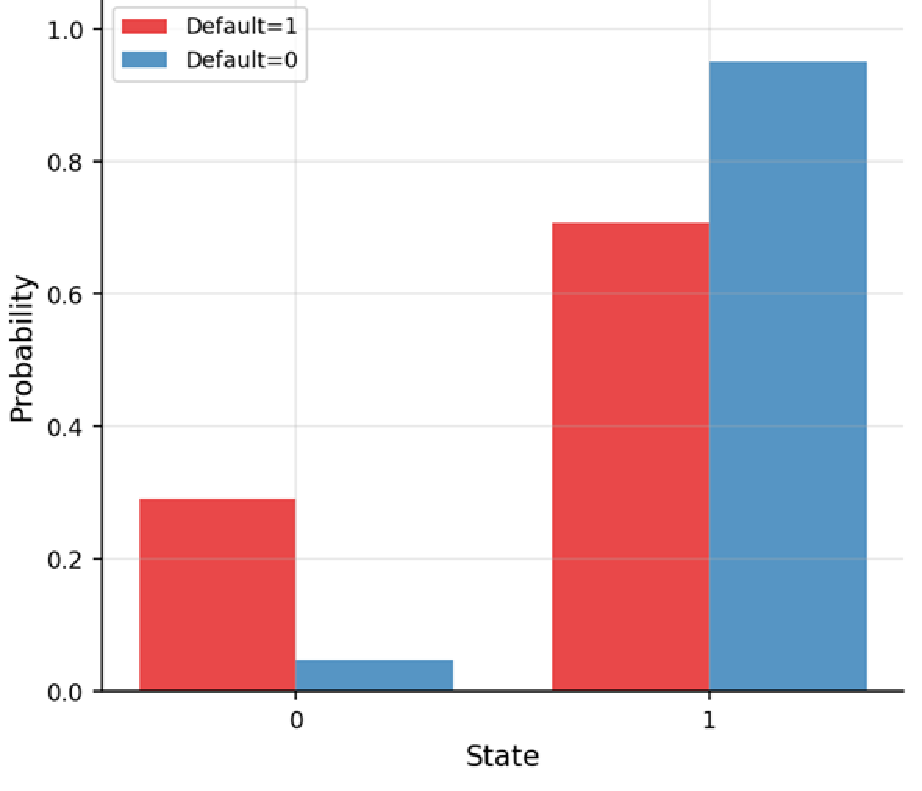
\includegraphics[width=\textwidth]{image/backward/backward_ger_foreign.pdf}\\[0.1cm]
            \caption{\texttt{is\_foreign\_worker}}
        \end{minipage}
        \hfill
        \begin{minipage}{0.49\textwidth}
            \centering
            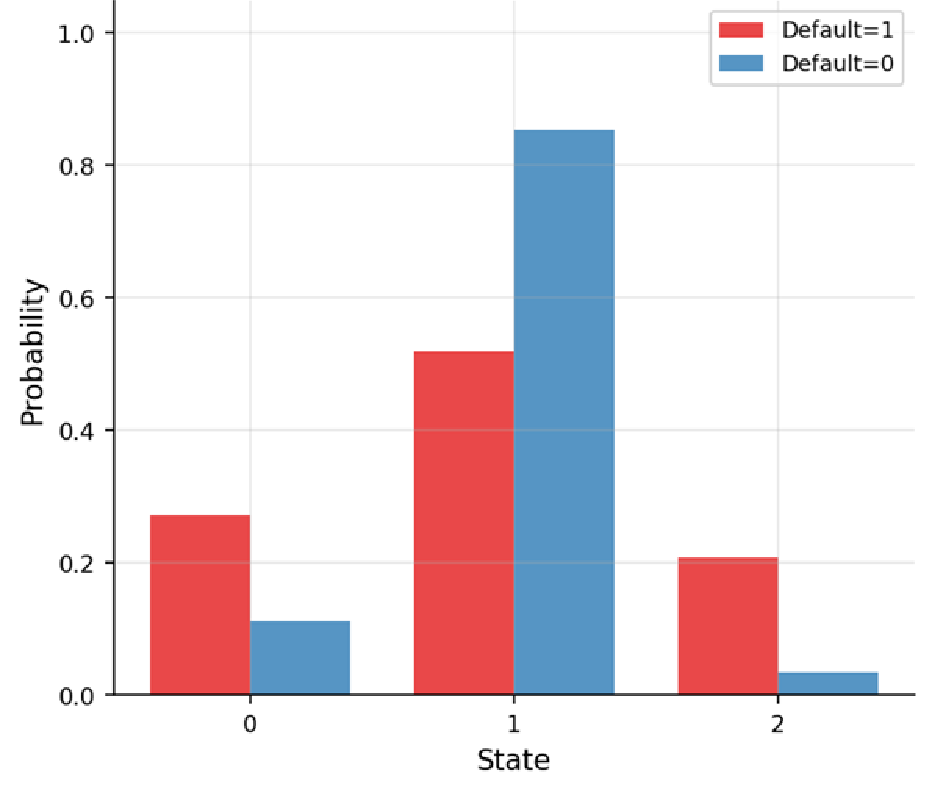
\includegraphics[width=\textwidth]{image/backward/backward_ger_otherins.pdf}\\[0.1cm]
            \caption{\texttt{other\_installment\_plans}}
        \end{minipage}
    \end{subfigure}
    \caption{Suy luận lùi trên các biến cha trực tiếp của \texttt{target} --- German Credit}
    \label{fig:backward_ger}
\end{figure}

Trên Lending Club, \texttt{int\_rate} và \texttt{grade} là hai biến cha được truy vấn ở Hình \ref{fig:backward_lend}. Đối với \texttt{int\_rate}, \textit{bin} lãi suất cao nhất chiếm $20.13\%$ trong nhóm vỡ nợ so với chỉ $9.01\%$ ở nhóm không vỡ nợ, trong khi \textit{bin} lãi suất thấp nhất lại phổ biến hơn hẳn ở nhóm không vỡ nợ ($25.05\%$) so với nhóm vỡ nợ ($7.29\%$), nhất quán với chiều tác động thuận đã ghi nhận ở Mục \ref{sec:4.4.1} và \ref{sec:4.4.2}. Đối với \texttt{grade}, tỷ trọng trong nhóm vỡ nợ tăng dần đều theo hạng tín dụng xấu dần, từ $3.08\%$ ở hạng A lên đến $33.47\%$ ở hạng C trước khi giảm dần ở các hạng thấp hơn do quy mô mẫu nhỏ, trong khi tỷ trọng ở nhóm không vỡ nợ lại tập trung nhiều nhất ở hạng B ($31.04\%$) và giảm dần về sau cho thấy phân phối \texttt{grade} của nhóm vỡ nợ lệch rõ rệt về phía các hạng tín dụng kém hơn so với nhóm không vỡ nợ.

\begin{figure}[H]
    \centering
    \begin{subfigure}[b]{\textwidth}
        \centering
        \begin{minipage}{0.49\textwidth}
            \centering
            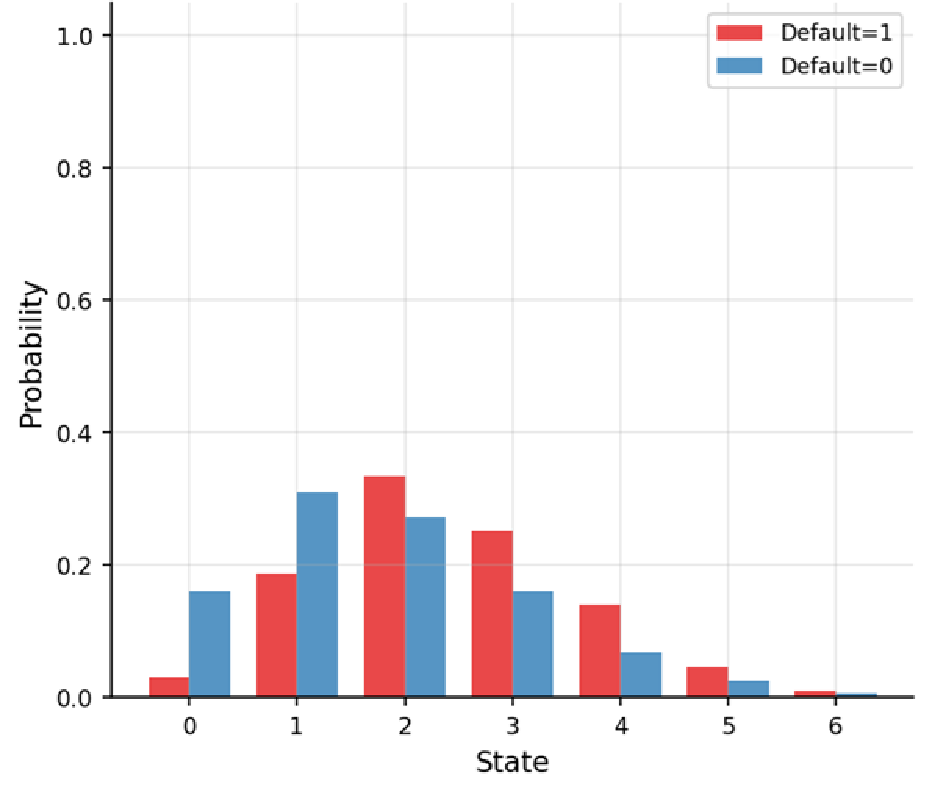
\includegraphics[width=\textwidth]{image/backward/backward_lend_grade.pdf}\\[0.1cm]
            \caption{\texttt{grade}}
        \end{minipage}
        \hfill
        \begin{minipage}{0.49\textwidth}
            \centering
            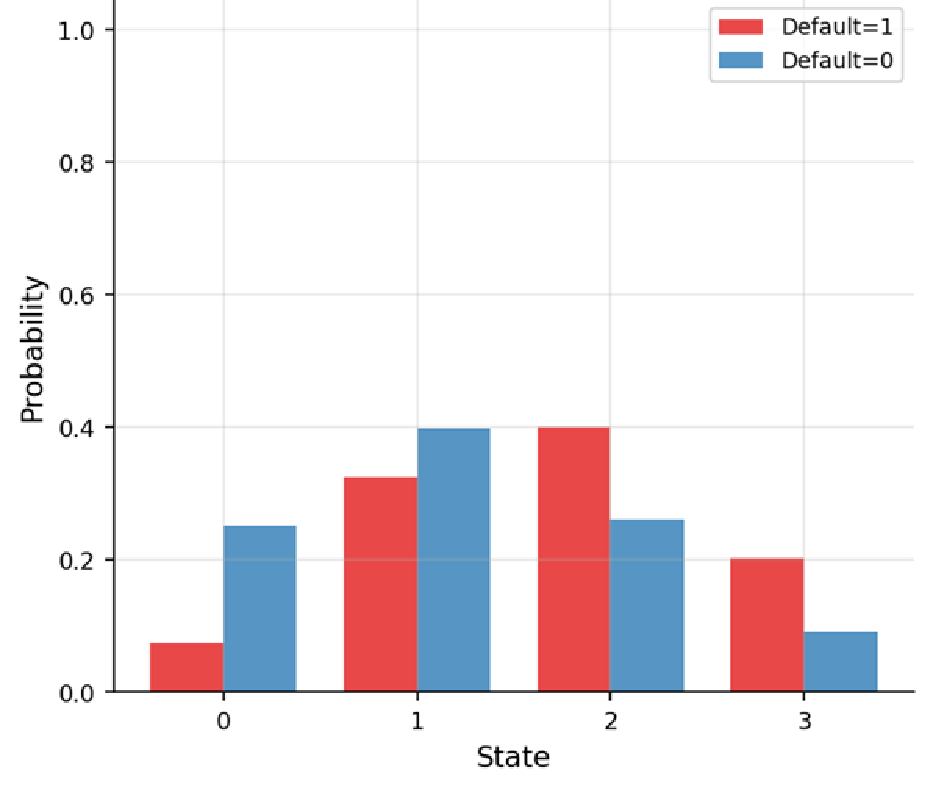
\includegraphics[width=\textwidth]{image/backward/backward_lend_int.pdf}\\[0.1cm]
            \caption{\texttt{int\_rate}}
        \end{minipage}
    \end{subfigure}
    \caption{Suy luận lùi trên các biến cha trực tiếp của \texttt{target} --- Lending Club}
    \label{fig:backward_lend}
\end{figure}
Để có cái nhìn toàn cục hơn thay vì chỉ giới hạn ở các biến cha, suy luận lùi còn được mở rộng ra toàn bộ các nút của mạng: gán \texttt{target}=0 và \texttt{target}=1 lần lượt làm evidence, sau đó truy vấn lại phân phối hậu nghiệm của mọi biến còn lại, thể hiện tại Hình \ref{fig:backward_australian}, \ref{fig:backward_german} và  \ref{fig:backward_lendingclub} mỗi hình gồm hai đồ thị ứng với \texttt{target} = 0 và \texttt{target} = 1.

\begin{figure}[H]
    \centering
    \begin{subfigure}[b]{\textwidth}
        \centering
        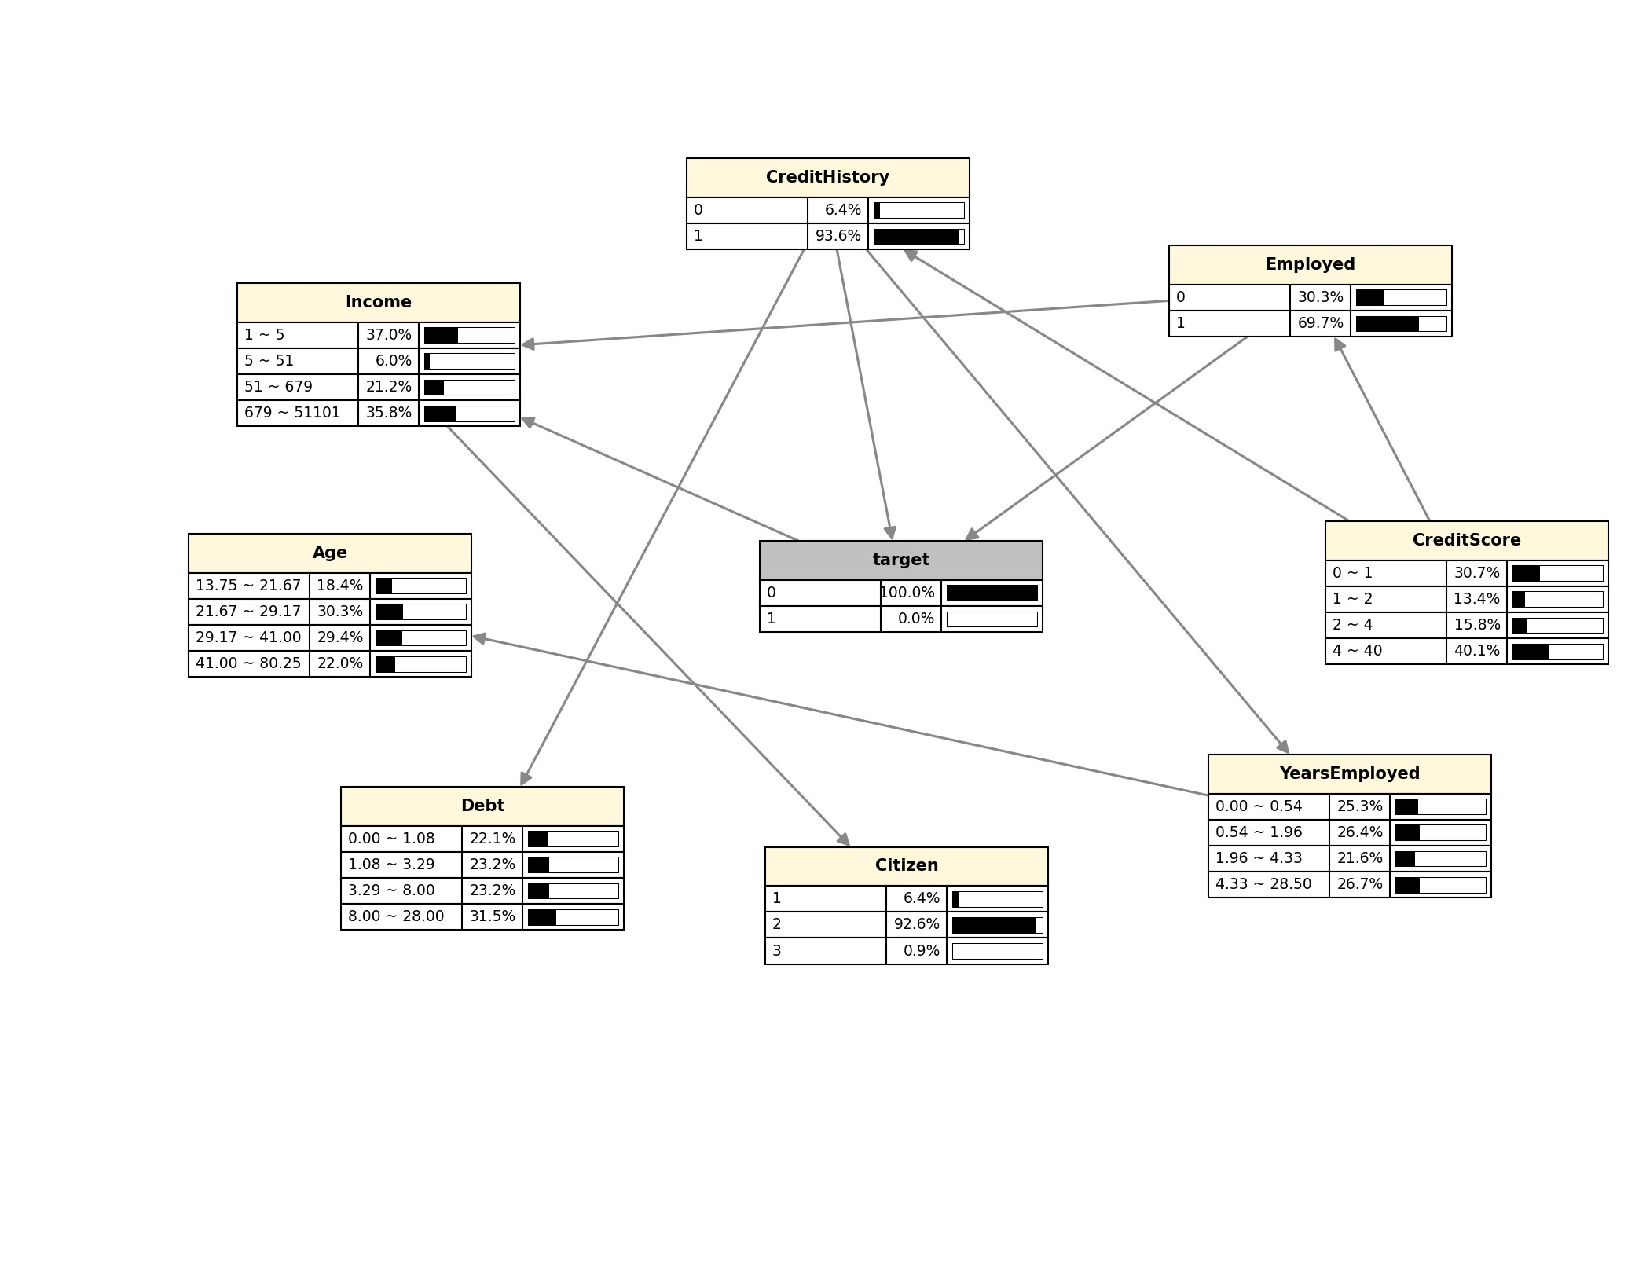
\includegraphics[width=1.05\textwidth,
        height=0.43\textheight,
        trim=3cm 5cm 0cm 2.5cm,
        clip
        ]{image/backward/au_back_0.pdf}
        \caption{target = 0}
        \label{fig:au_back_0}
    \end{subfigure}
    \caption{Suy luận lùi toàn cục theo evidence target --- Australian Credit}
\end{figure}
    
\begin{figure}
    \ContinuedFloat
    \centering
    \begin{subfigure}[b]{\textwidth}
        \centering
        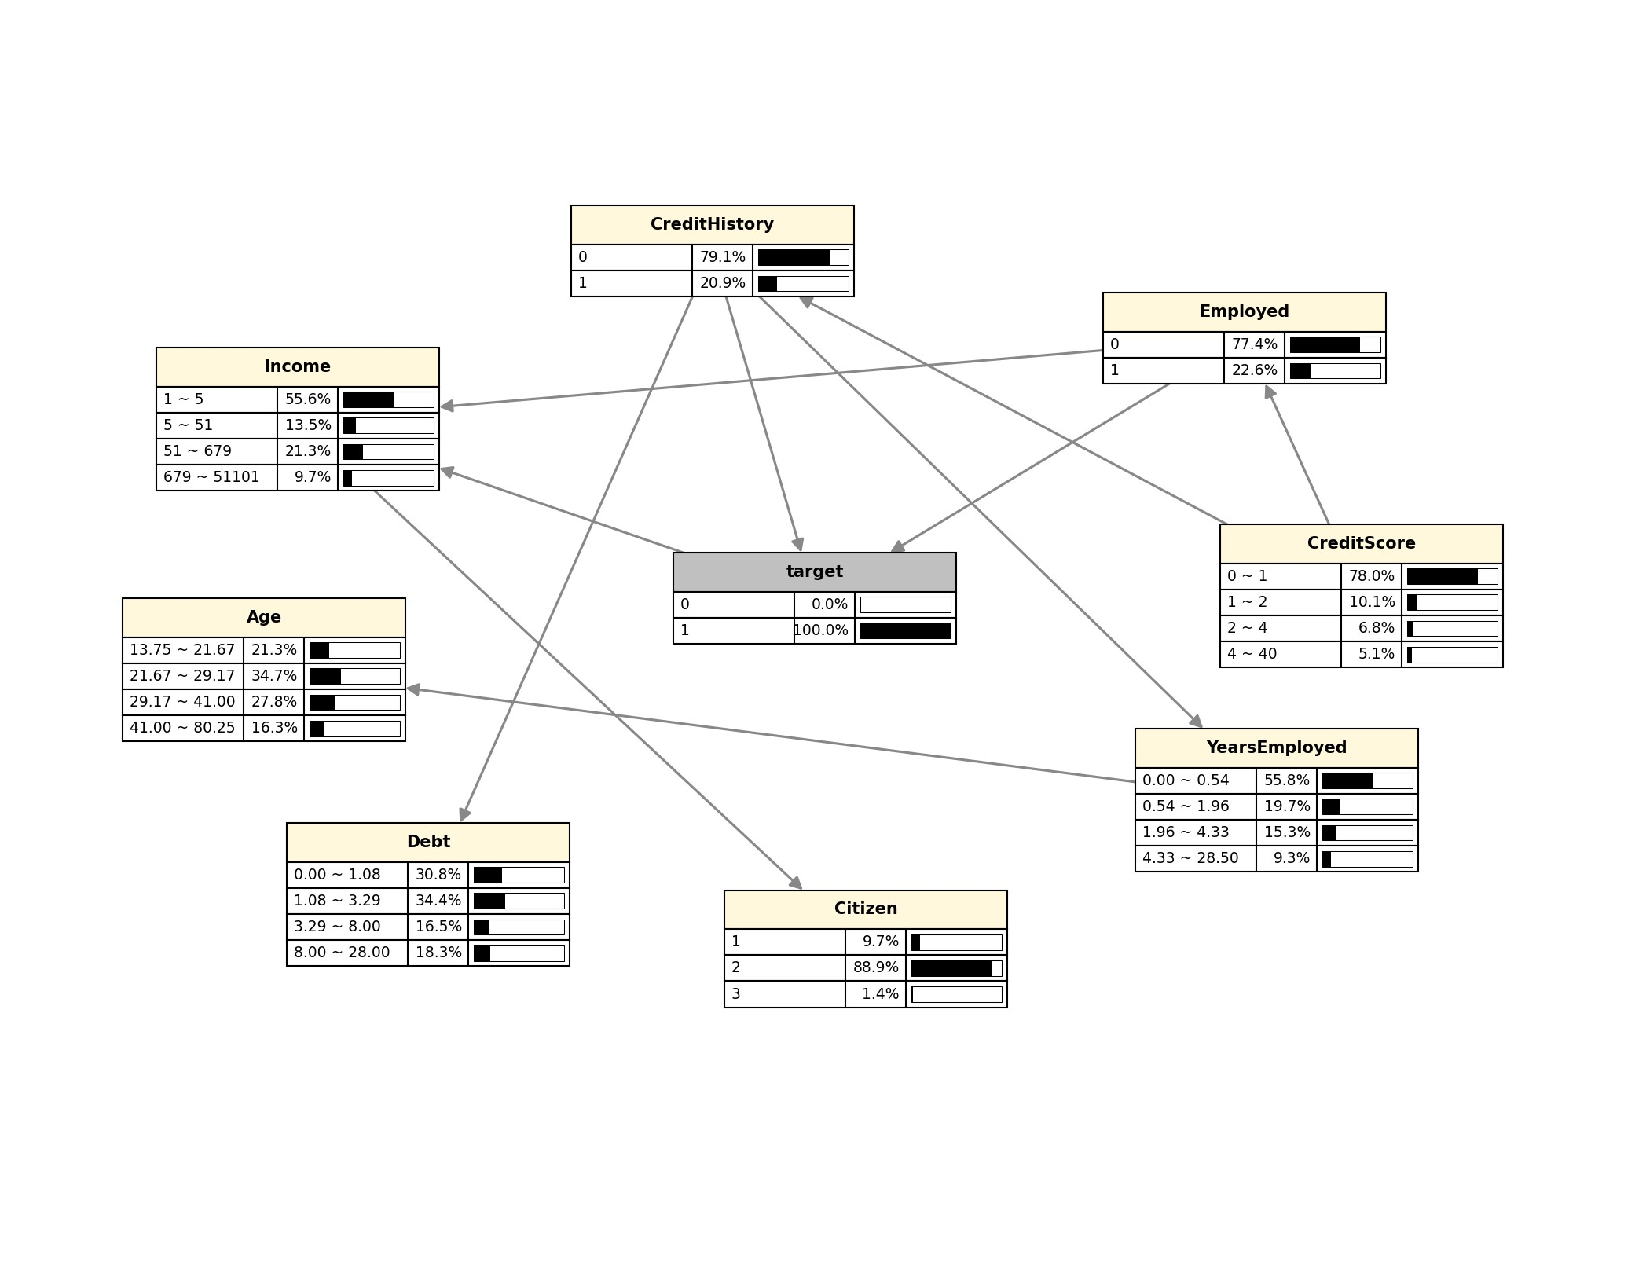
\includegraphics[width=1.1\textwidth,
        height=0.5\textheight,
        trim=2cm 4cm 0cm 3cm,
        clip]{image/backward/au_back_1.pdf}
        \caption{target = 1}
        \label{fig:au_back_1}
    \end{subfigure}
    \caption{Suy luận lùi toàn cục theo evidence target --- Australian Credit (tiếp theo)}
    \label{fig:backward_australian}
\end{figure}


Trên Australian Credit, \texttt{CreditHistory} dịch chuyển mạnh nhất trong toàn mạng (Hình \ref{fig:backward_australian}): từ tiên nghiệm 42.9\%/57.1\% (không/có lịch sử) lệch hẳn về 79.1\%/20.9\% khi \texttt{target}=1 và ngược lại về 6.4\%/93.6\% khi \texttt{target}=0. \texttt{Employed} cũng dịch chuyển đáng kể (53.9\%/46.1\% tiên nghiệm $\rightarrow$ 77.4\%/22.6\% khi vỡ nợ $\rightarrow$ 30.3\%/69.7\% khi không vỡ nợ), trong khi \texttt{Citizen} hầu như không đổi qua cả ba kịch bản (dao động trong khoảng 1 điểm phần trăm), củng cố nhận định rằng đây là biến ít liên quan đến rủi ro tín dụng dù vẫn nằm trong tập đặc trưng được chọn.


Trên German Credit, ba biến dịch chuyển rõ rệt nhất (Hình \ref{fig:backward_german}) là \texttt{credit\_history}, \texttt{other\_installment\_plans} và \texttt{secondary\_obligor}. Đáng chú ý nhất là \texttt{secondary\_obligor}: trạng thái "guarantor" (có người bảo lãnh) chiếm 73.2\% ở phân phối tiên nghiệm, tăng lên 89.7\% ở nhóm không vỡ nợ nhưng giảm còn 56.7\% ở nhóm vỡ nợ cho thấy sự hiện diện của người bảo lãnh có vai trò bảo vệ rõ rệt trên quy mô toàn mạng chứ không chỉ trong quan hệ trực tiếp với \texttt{is\_foreign\_worker} đã phân tích trước đó. Tương tự, \texttt{other\_installment\_plans} lệch từ 68.7\% (trạng thái "stores" ở tiên nghiệm) lên 85.4\% ở nhóm không vỡ nợ nhưng chỉ còn 51.9\% ở nhóm vỡ nợ.

Trên Lending Club, dịch chuyển đáng chú ý nhất và mang tính chẩn đoán cao nhất toàn mạng (Hình \ref{fig:backward_lendingclub}) là \texttt{debt\_settlement\_flag}: ở nhóm không vỡ nợ, biến này đạt 100\% tại trạng thái "không" tức trong dữ liệu, không có bất kỳ khách hàng không vỡ nợ nào từng tham gia chương trình tái cơ cấu nợ trong khi ở nhóm vỡ nợ tỷ lệ "có" tăng lên 4.0\% so với 2.0\% ở tiên nghiệm. \texttt{grade} và \texttt{int\_rate} cũng dịch chuyển nhất quán với các phân tích trước: nhóm vỡ nợ lệch hẳn về các hạng thấp và lãi suất cao (ví dụ hạng G tăng từ 0.8\% tiên nghiệm lên 1.0\%, trong khi hạng A giảm từ 9.6\% xuống 3.1\%), còn nhóm không vỡ nợ lệch ngược lại về phía hạng A và lãi suất thấp (hạng A tăng lên 16.1\%, bin lãi suất thấp nhất tăng lên 25.0\%).

\begin{figure}[H]
    \centering
    \begin{subfigure}[b]{\textwidth}
        \centering
        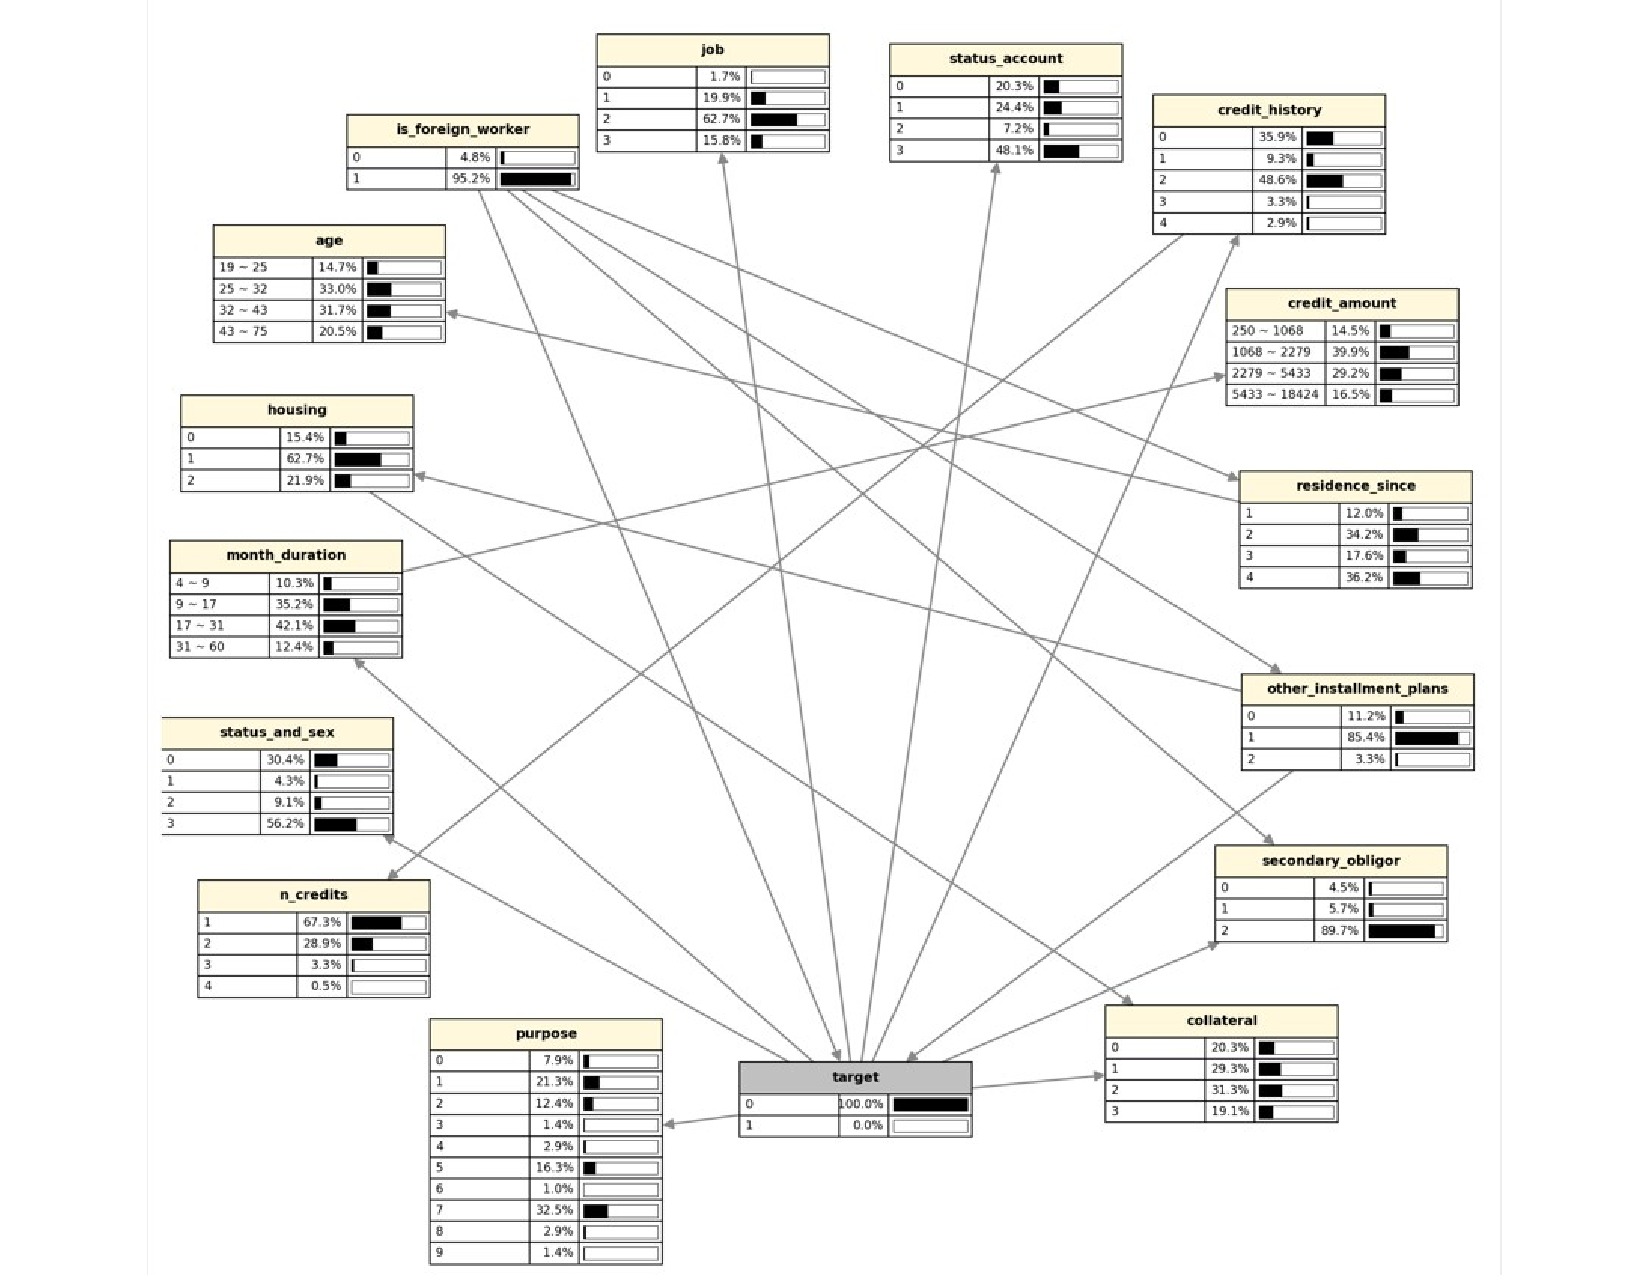
\includegraphics[width=1.2\textwidth,
        height=0.7\textheight,
        trim=1.5cm 0cm 0cm 0.5cm,
        clip]{image/backward/ger_back_0.pdf}
        \caption{target = 0}
        \label{fig:ger_back_0}
    \end{subfigure}
    \caption{Suy luận lùi toàn cục theo evidence target --- German Credit}
\end{figure}

 \begin{figure}[H]
    \ContinuedFloat
    \centering   
    \begin{subfigure}[b]{\textwidth}
        \centering
        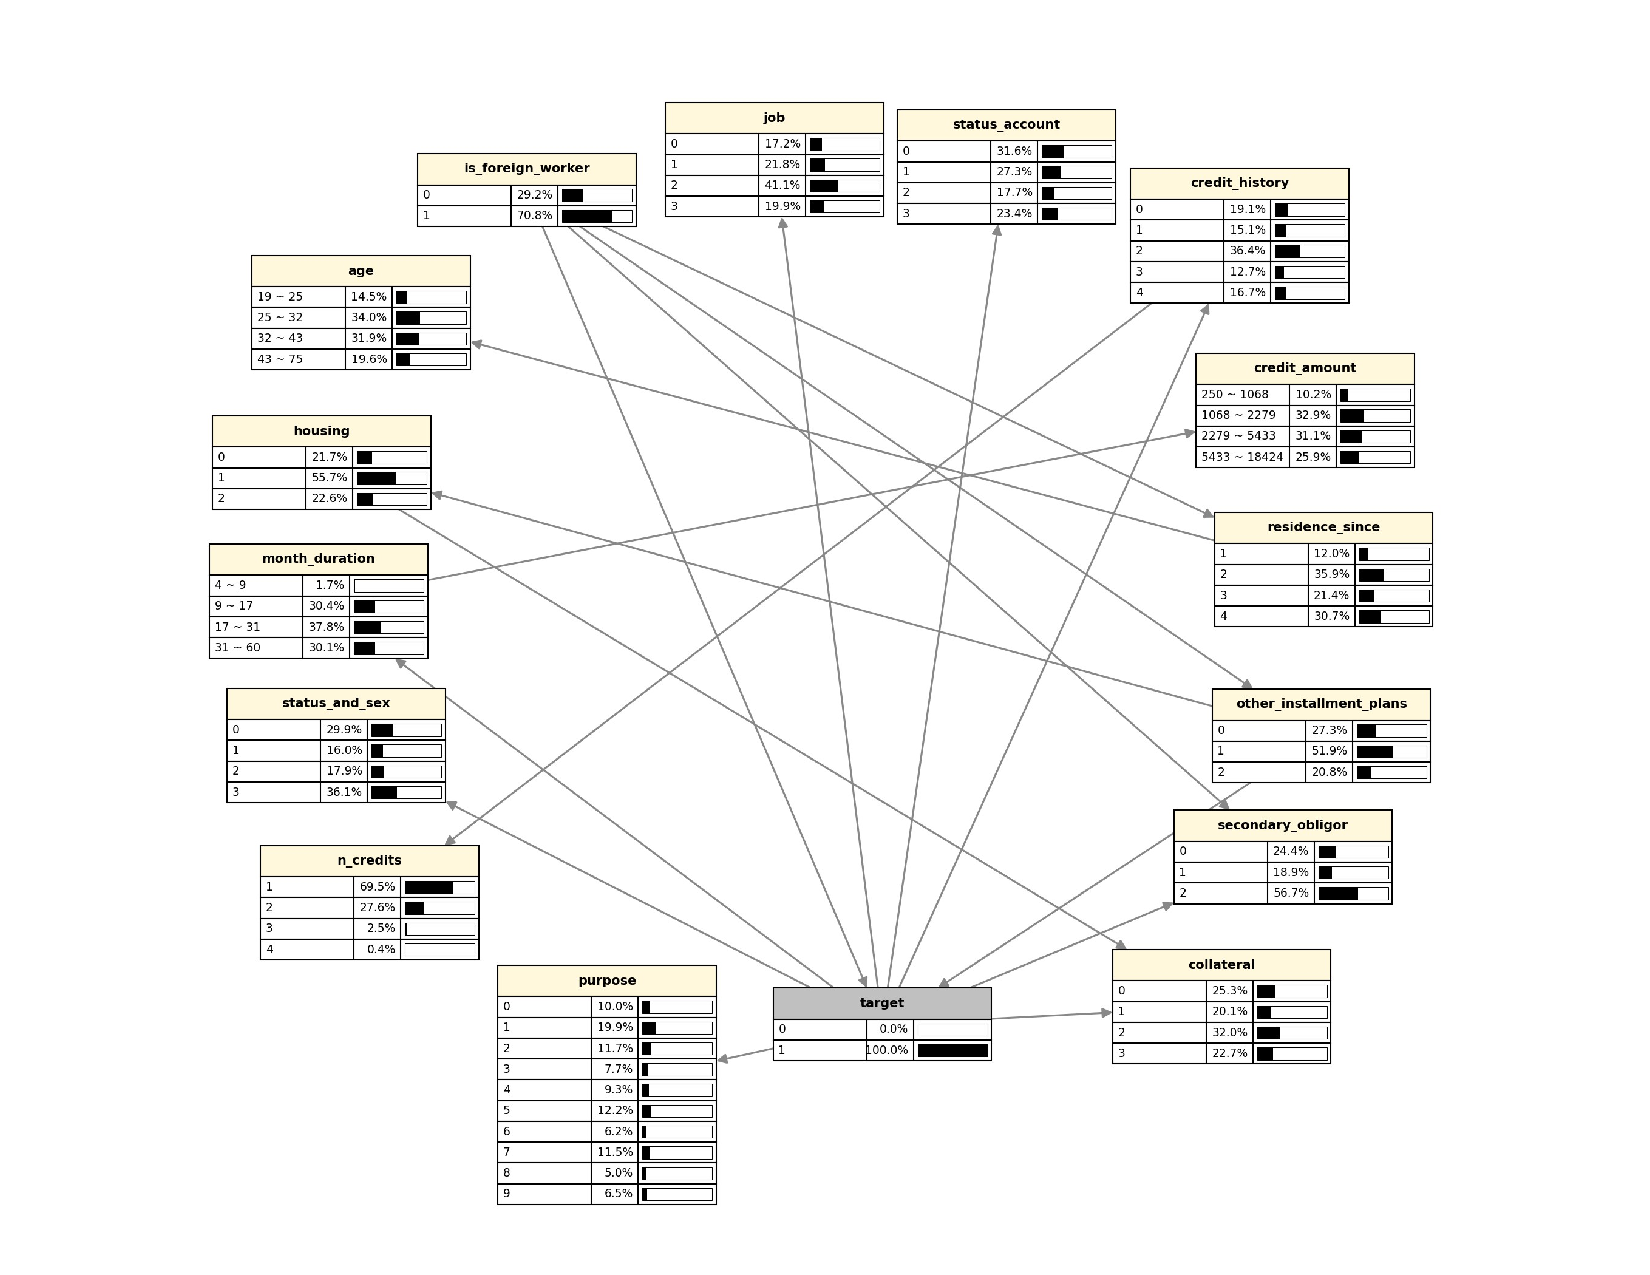
\includegraphics[width=1.2\textwidth,
        height=0.7\textheight,
        trim=3cm 1cm 0cm 1cm,
        clip]{image/backward/ger_back_1.pdf}
        \caption{target = 1}
        \label{fig:ger_back_1}
    \end{subfigure}
    \caption{Suy luận lùi toàn cục theo evidence target --- German Credit (tiếp theo)}
    \label{fig:backward_german}
\end{figure}


Kết quả suy luận lùi toàn cục này nhất quán hoàn toàn với các phát hiện cục bộ đã trình bày ở phần trên, đồng thời cho thấy rõ hơn mức độ lan tỏa của bằng chứng \texttt{target} qua toàn bộ cấu trúc mạng.

Tổng hợp cả ba bộ dữ liệu, suy luận lùi cung cấp một góc nhìn bổ trợ quan trọng so với hai kỹ thuật trước: thay vì trả lời ``một hồ sơ cụ thể có rủi ro bao nhiêu'', nó trả lời ``một nhóm hồ sơ đã biết kết quả thường có đặc điểm gì'', phục vụ trực tiếp cho bài toán truy vết hồ sơ và xây dựng chân dung rủi ro sau khi đã quan sát được kết quả vỡ nợ trên thực tế.


\begin{figure}[p]
    \centering
    \begin{subfigure}[b]{\textwidth}
        \centering
    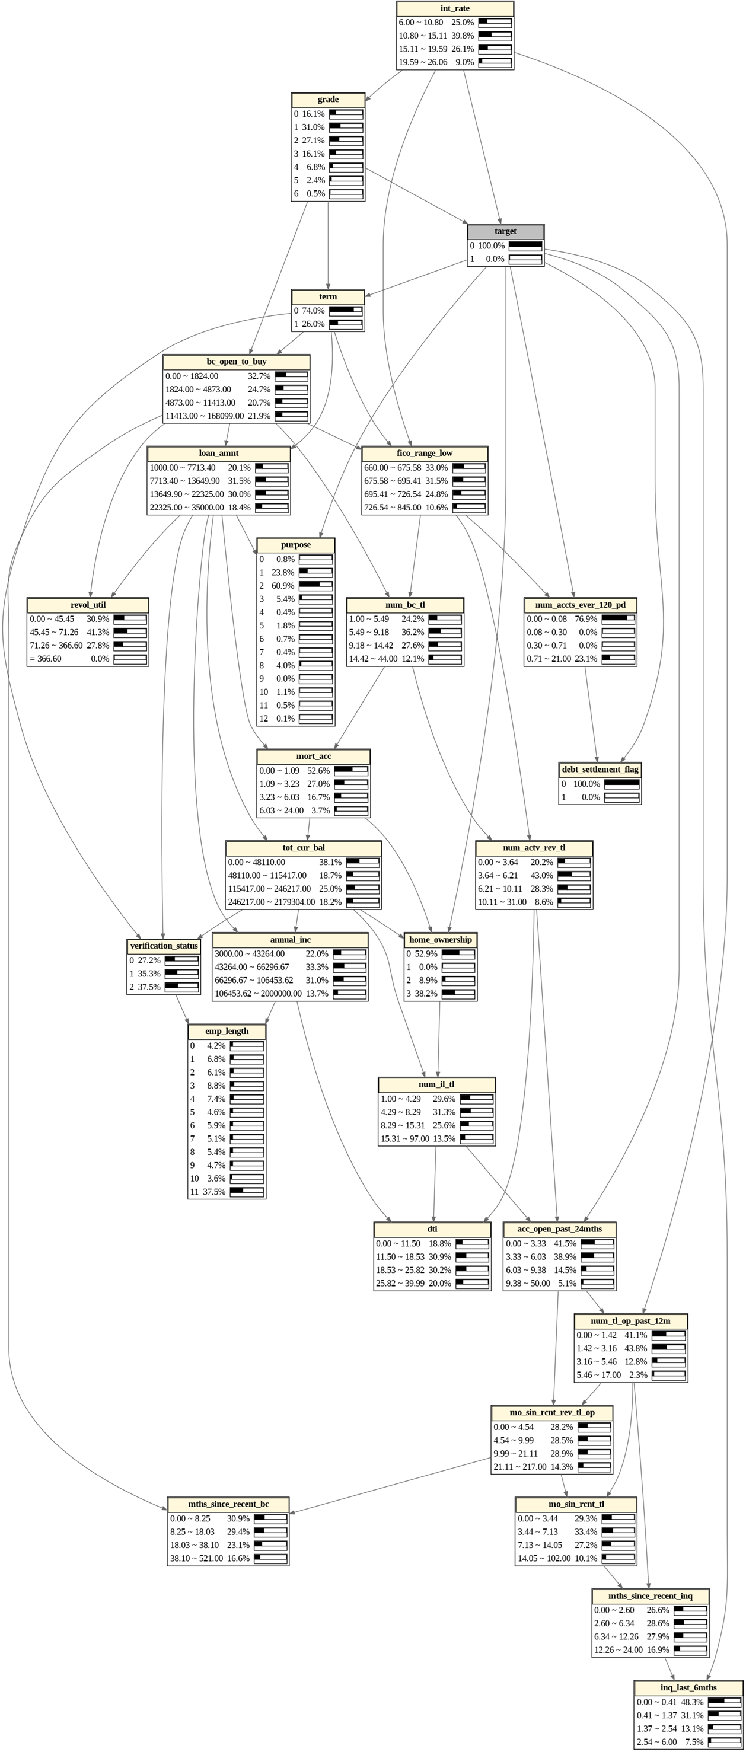
\includegraphics[width=\textwidth,height=\textheight]{image/backward/lend_back_0.pdf}
        \caption{target = 0}
        \label{fig:lend_back_0}
    \end{subfigure}
    \caption{Suy luận lùi toàn cục theo evidence target --- Lending Club}
\end{figure}

\begin{figure}[p]
    \ContinuedFloat
    \centering
    \begin{subfigure}[b]{\textwidth}
        \centering    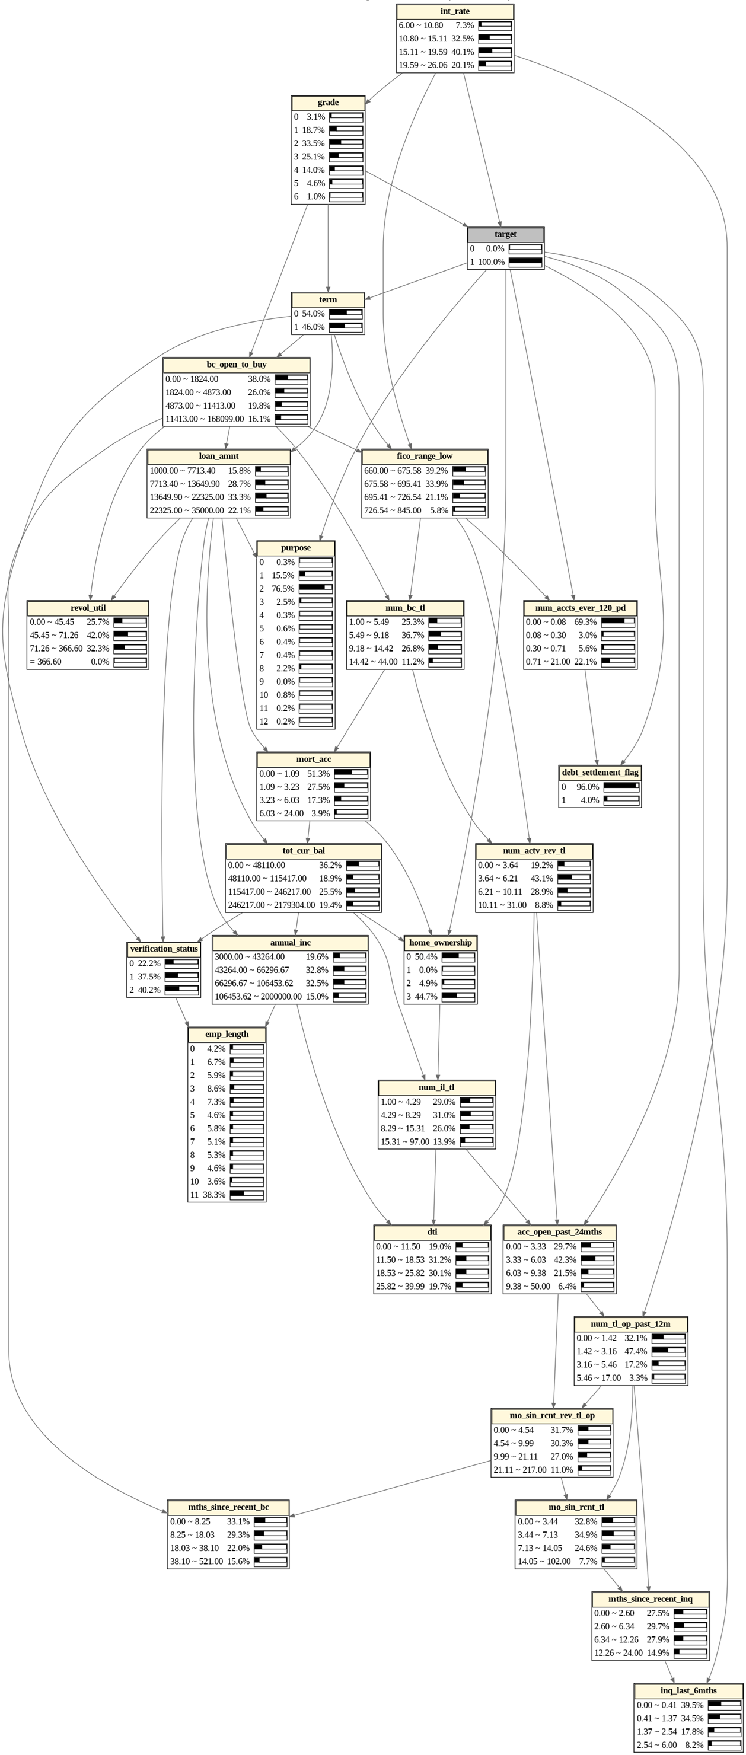
\includegraphics[width=\textwidth,height=\textheight]{image/backward/lend_back_1.pdf}
        \caption{target = 1}
        \label{fig:lend_back_1}
    \end{subfigure}
    \caption{Suy luận lùi toàn cục theo evidence target --- Lending Club (tiếp theo)}
    \label{fig:backward_lendingclub}
\end{figure}

\newpage
\subsubsection{Phân tích kịch bản giả định}
\noindent
Hai cách tiếp cận được triển khai song song để phân tích kịch bản giả định: một cách xét trên hồ sơ cá nhân cụ thể, một cách xét trên cấu trúc con của mạng.

\paragraph{Kịch bản theo hồ sơ cá nhân (Persona-based)}\\

Với mỗi bộ dữ liệu, một vài biến nhân khẩu học không thể can thiệp được cố định làm hồ sơ neo (Australian: \texttt{Age}, \texttt{Citizen}; German: \texttt{age}, \texttt{status\_and\_sex}, \texttt{housing}; Lending Club: \texttt{annual\_inc}, \texttt{fico\_range\_low}, \texttt{mort\_acc}), sau đó lần lượt thay đổi từng biến trong nhóm ba biến nhạy cảm nhất và quan sát $\Delta P(\text{target}=1)$ so với baseline của hồ sơ neo đó.


\begin{figure}[H]
\centering
\begin{subfigure}[b]{\textwidth}
    \centering
    \begin{subfigure}[b]{0.45\textwidth}
        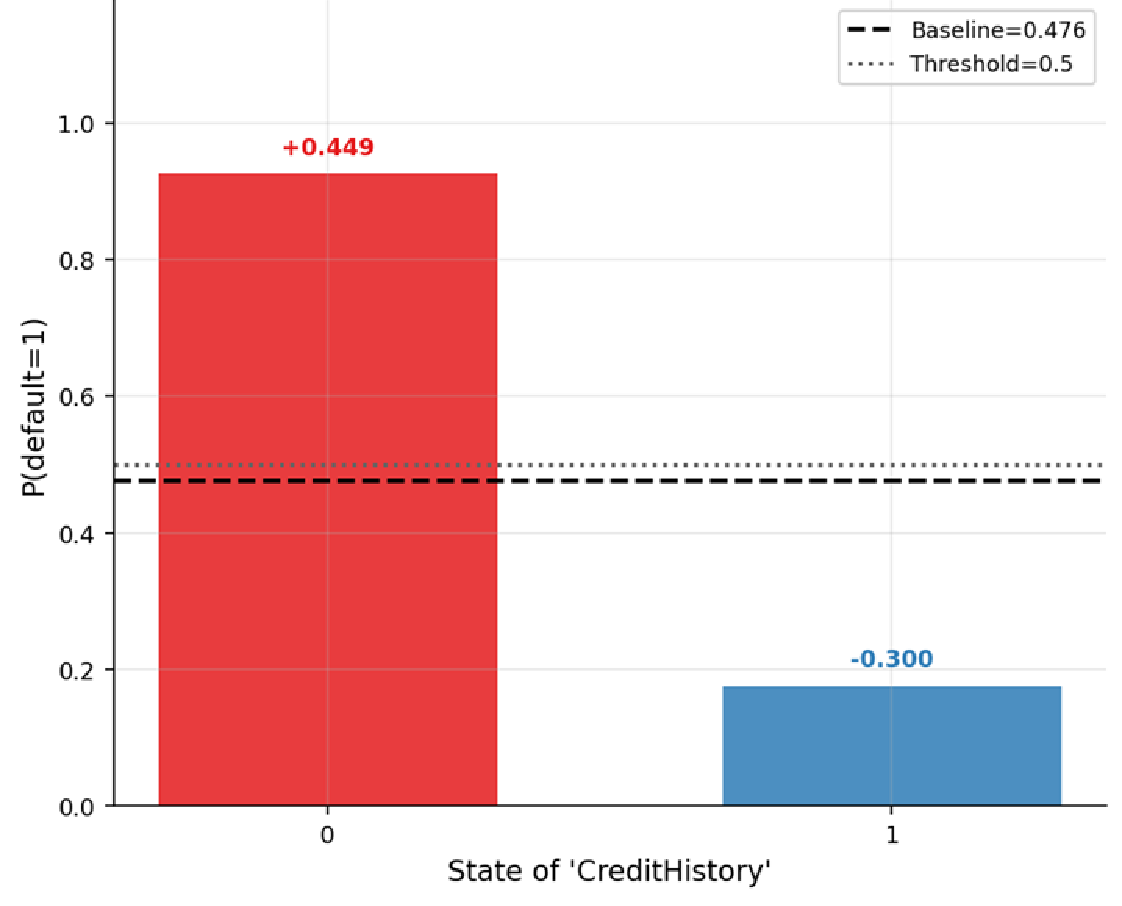
\includegraphics[width=\textwidth]{image/whatif/persona/au_1_crehis.pdf}
    \end{subfigure}
    \hfill
    \begin{subfigure}[b]{0.45\textwidth}
        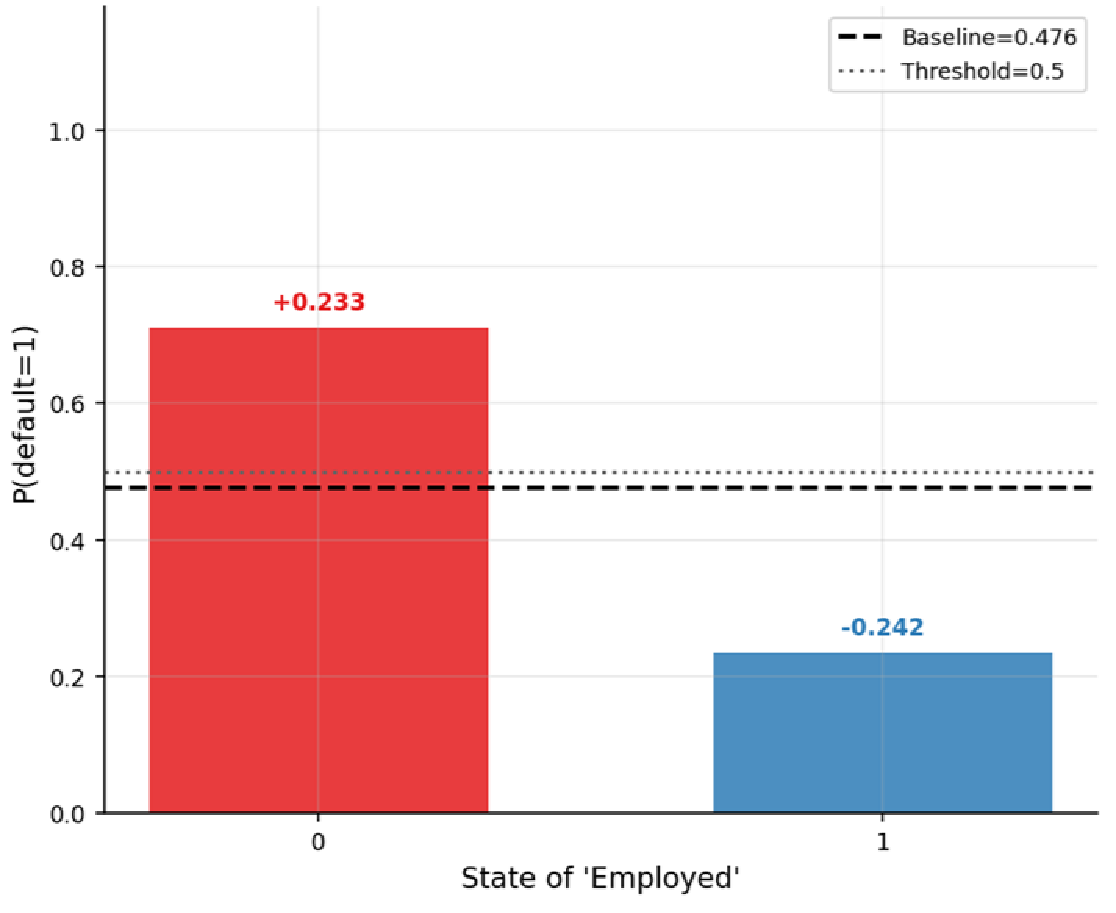
\includegraphics[width=\textwidth]{image/whatif/persona/au_1_employ.pdf}
    \end{subfigure}
    \hfill
    \begin{subfigure}[b]{0.45\textwidth}
        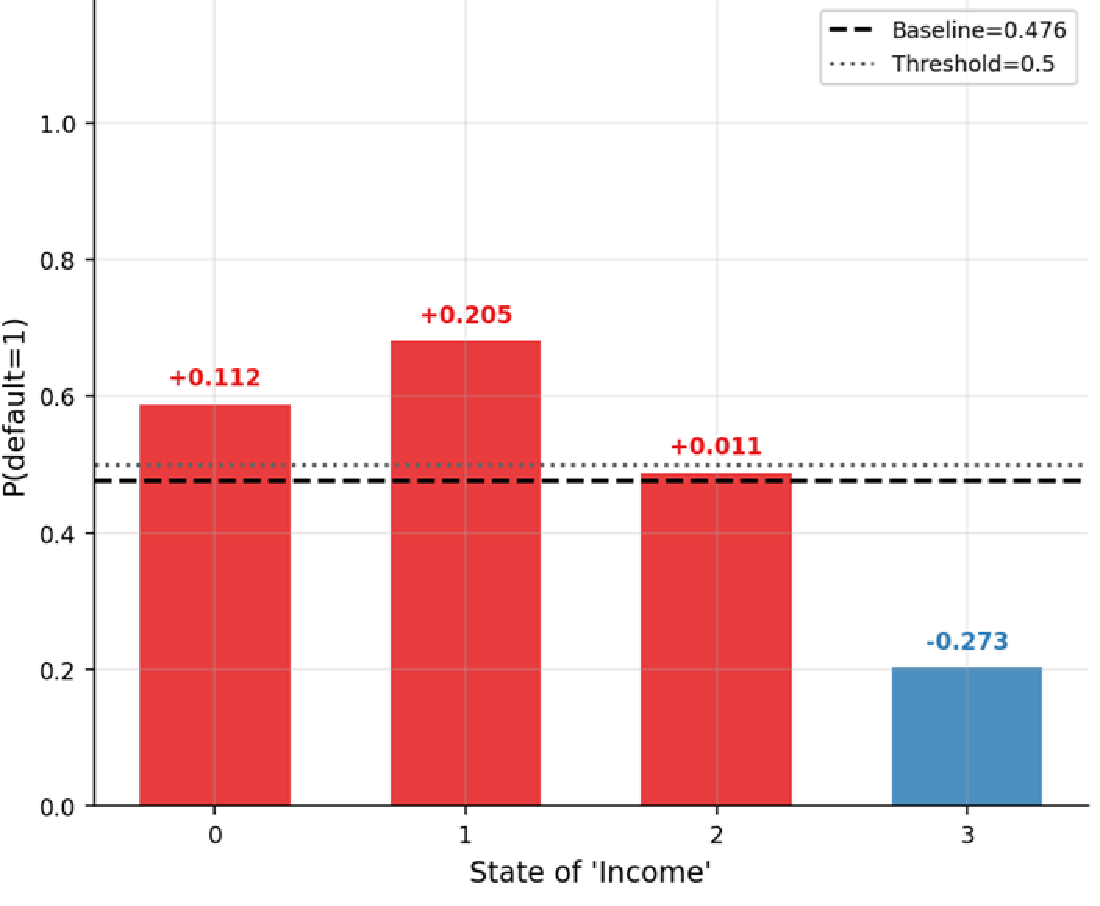
\includegraphics[width=\textwidth]{image/whatif/persona/au_1_inc.pdf}
    \end{subfigure}   
\end{subfigure}

\caption{Phân tích kịch bản giả định theo hồ sơ cá nhân --- Australian Credit {\newline \small (Trong đó, màu xanh: target = 0 và màu đỏ: target = 1})}
\label{fig:whatif_australian}
\end{figure}

Trên Australian Credit, baseline của hồ sơ neo là 47.64\%. Khi \texttt{CreditHistory} chuyển từ "không có" sang "có", xác suất vỡ nợ giảm từ 92.54\% xuống 17.68\% ($\Delta P = -0.300$). \texttt{Employed} cho biên độ nhỏ hơn, giảm từ 70.95\% xuống 23.45\% ($\Delta P = -0.242$) khi chuyển sang có việc làm. \texttt{Income} lại không đơn điệu như đã ghi nhận ở Mục \ref{sec:4.4.1}: xác suất tăng nhẹ từ bin 0 (58.80\%) lên đỉnh ở bin 1 (68.12\%) trước khi giảm dần về bin 3 (20.31\%) (Hình \ref{fig:whatif_australian}).


\begin{figure}[H]
\centering
\begin{subfigure}[b]{\textwidth}
    \centering
    \begin{subfigure}[b]{0.6\textwidth}
        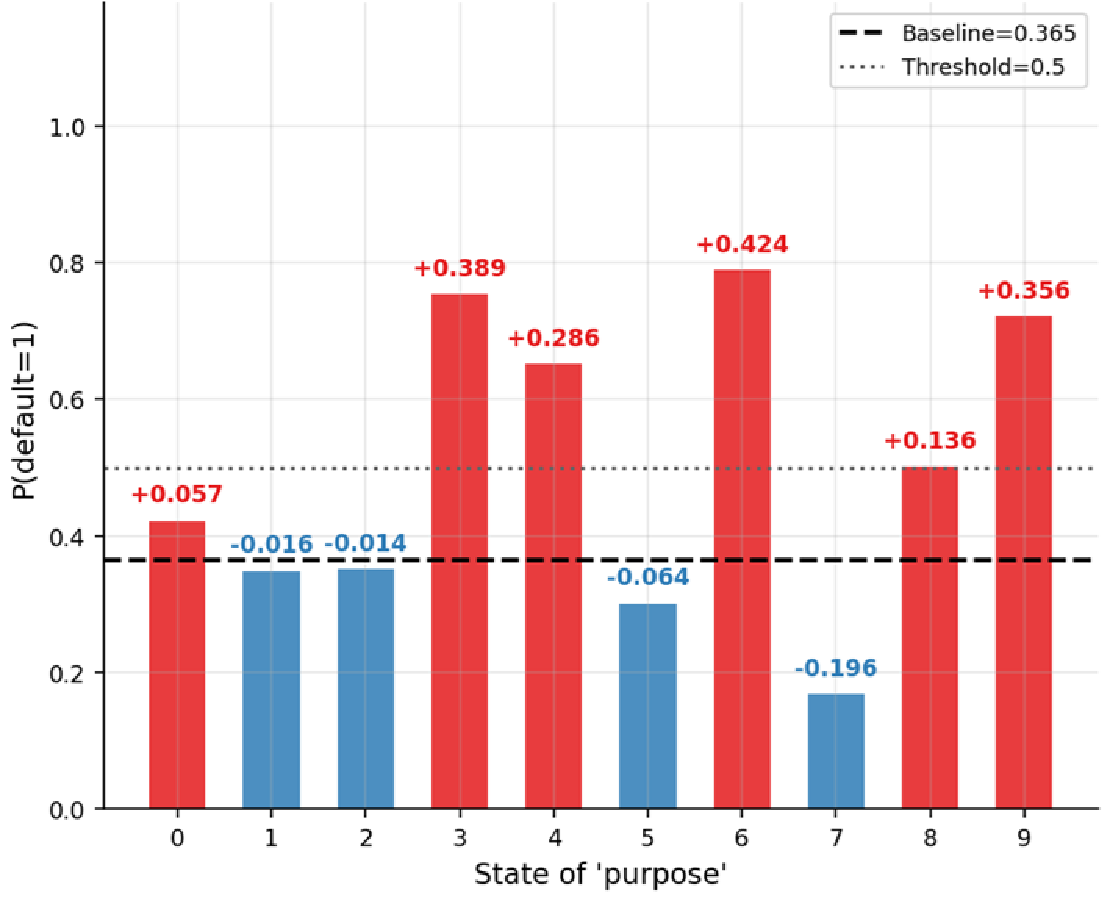
\includegraphics[width=\textwidth]{image/whatif/persona/ger_1_purpose.pdf}
    \end{subfigure}
    \hfill
    \begin{subfigure}[b]{0.6\textwidth}
        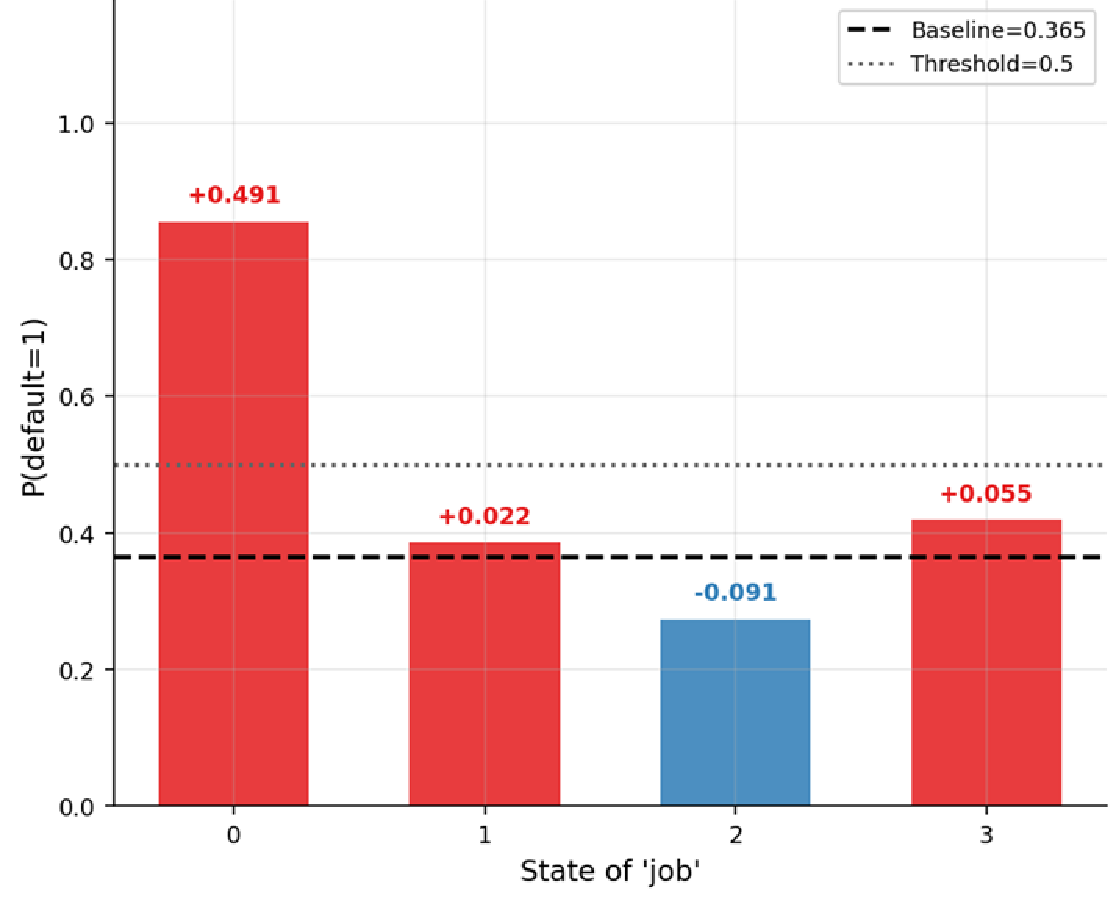
\includegraphics[width=\textwidth]{image/whatif/persona/ger_1_job.pdf}
    \end{subfigure}
    \hfill
    \begin{subfigure}[b]{0.6\textwidth}
        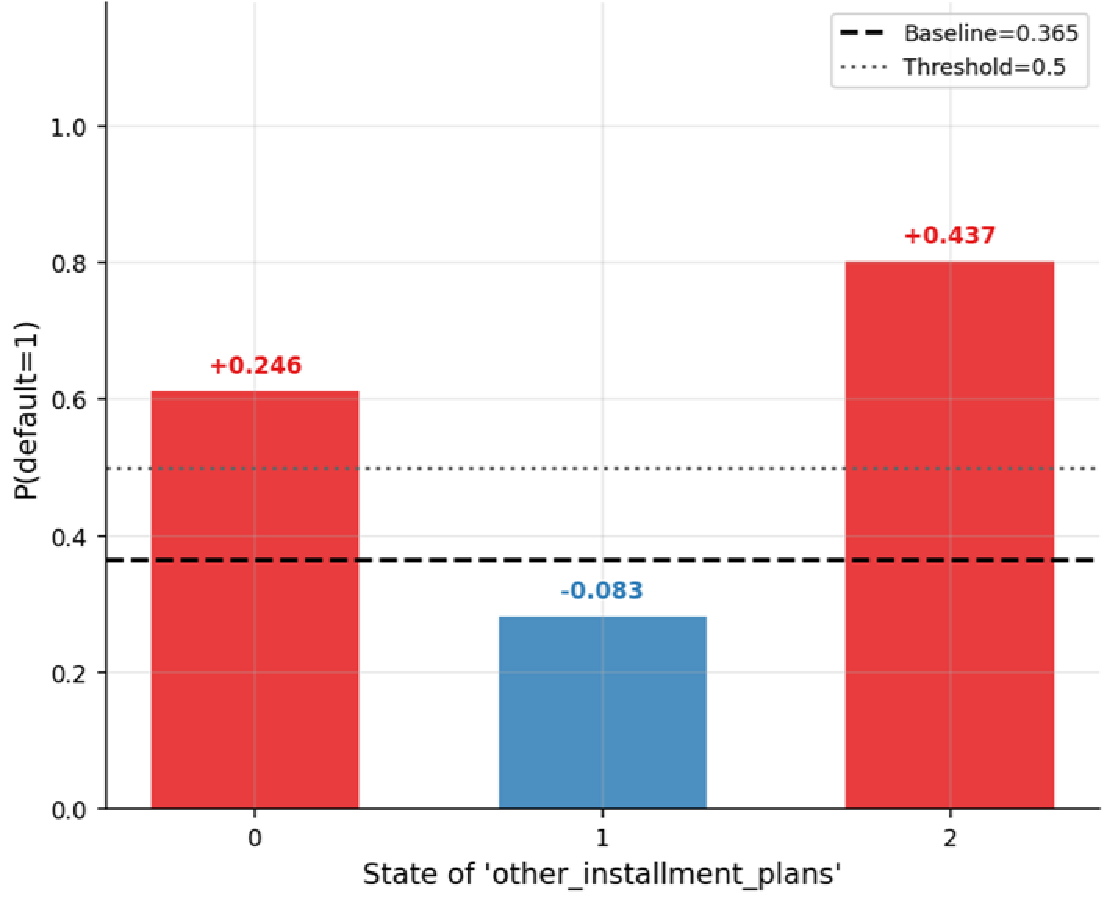
\includegraphics[width=\textwidth]{image/whatif/persona/ger_1_otherins.pdf}
    \end{subfigure}
    \label{fig:whatif_german}
\end{subfigure}

\caption{Phân tích kịch bản giả định theo hồ sơ cá nhân --- German Credit {\newline \small (Trong đó, màu xanh: target = 0 và màu đỏ: target = 1})}
\label{fig:whatif_german}
\end{figure}

\begin{figure}[H]
\centering
\begin{subfigure}[b]{\textwidth}
    \centering
    \begin{subfigure}[b]{0.6\textwidth}
        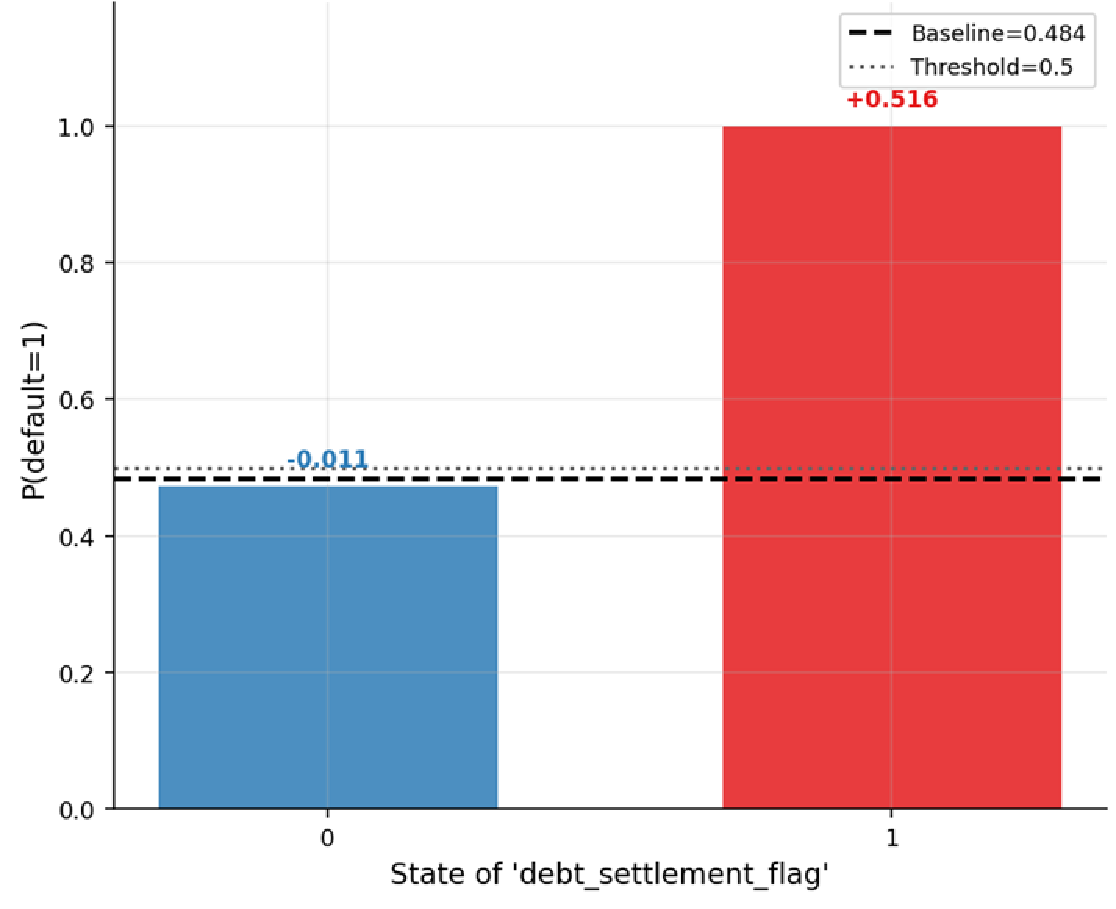
\includegraphics[width=\textwidth]{image/whatif/persona/lend_1_debt.pdf}
    \end{subfigure}
    \hfill
    \begin{subfigure}[b]{0.6\textwidth}
        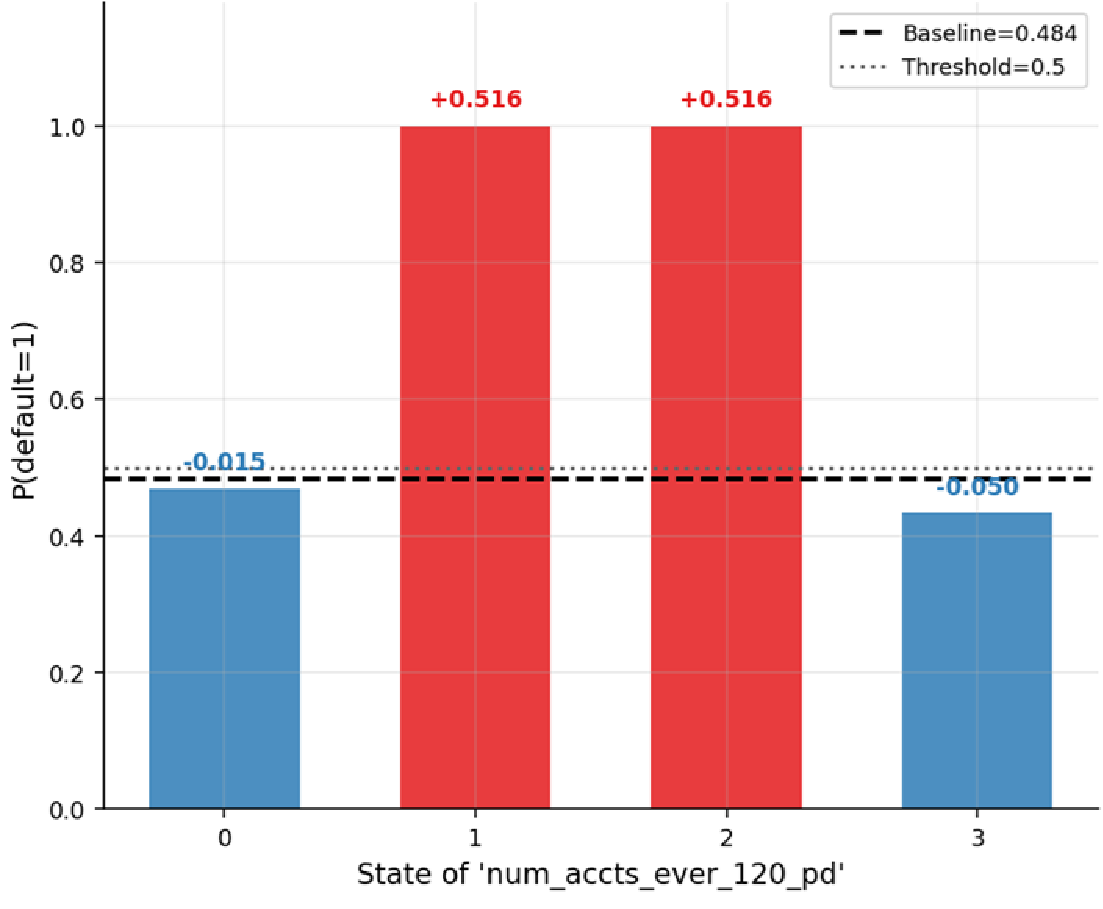
\includegraphics[width=\textwidth]{image/whatif/persona/lend_1_numacc.pdf}
    \end{subfigure}
    \hfill
    \begin{subfigure}[b]{0.6\textwidth}
        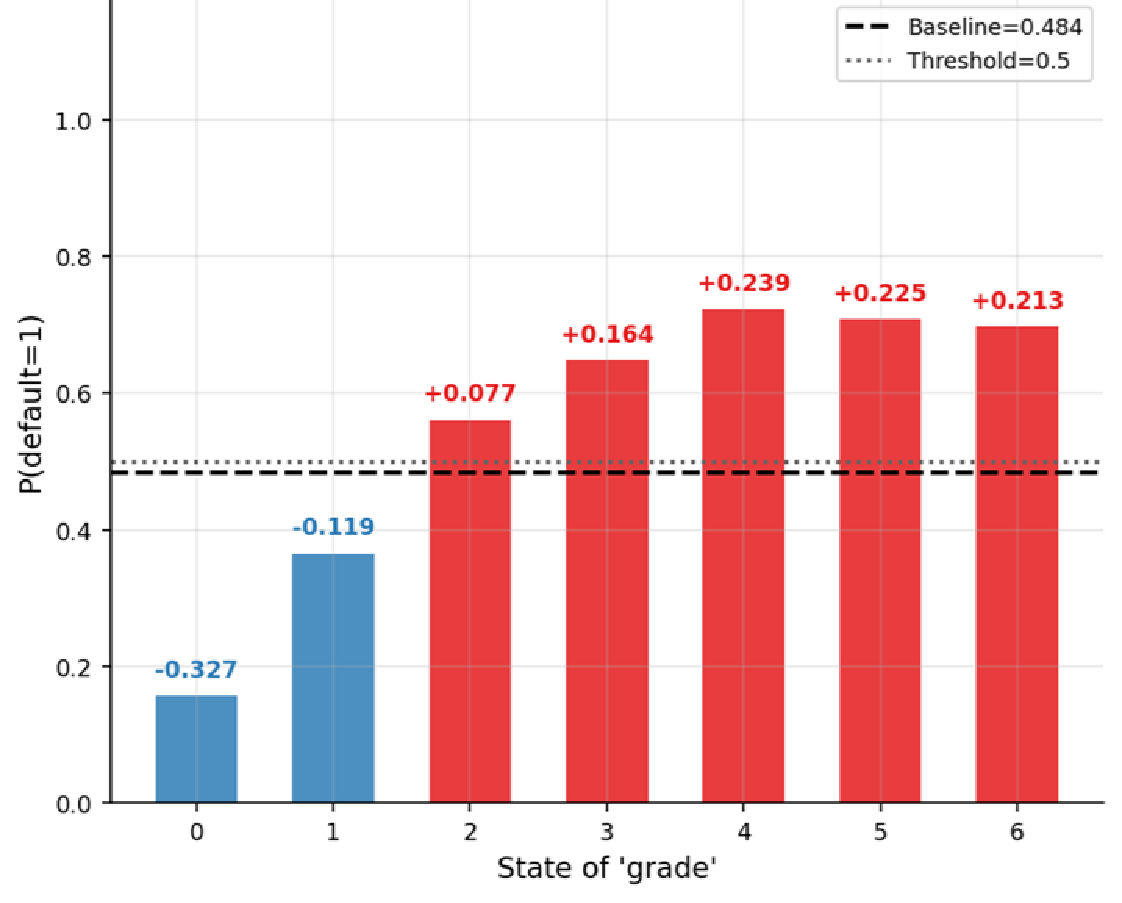
\includegraphics[width=\textwidth]{image/whatif/persona/lend_1_grade.pdf}
    \end{subfigure}
\end{subfigure}

\caption{Phân tích kịch bản giả định theo hồ sơ cá nhân --- Lending Club {\newline \small (Trong đó, màu xanh: target = 0 và màu đỏ: target = 1})}
\label{fig:whatif_lendingclub}
\end{figure}

Trên German Credit, baseline là 36.45\%. \texttt{Purpose} là biến có biên độ lớn nhất trong ba biến được khảo sát, dao động từ 16.84\% (bin 7) đến 78.85\% (bin 6), phản ánh sự phân hóa rủi ro rõ rệt theo từng mục đích vay cụ thể. \texttt{Job} dao động từ 27.35\% đến 85.51\%, trong đó bin 0 (thất nghiệp/không kỹ năng) mang rủi ro cao nhất. \texttt{Other\_installment\_plans} dao động từ 28.13\% (bin "stores") đến 80.10\% (bin "none"), tiếp tục thể hiện hình chữ V phi tuyến đã ghi nhận xuyên suốt các mục trước (Hình \ref{fig:whatif_german}).

Trên Lending Club, baseline là 48.39\%, \varname{num_accts_ever_120_pd} và \varname{Debt_settlement_flag} đều thể hiện biên độ cực đoan giống hệt kết quả $\delta = 0.5$ đã ghi nhận ở Mục \ref{sec:4.4.1}: chuyển sang trạng thái "có" khiến xác suất vỡ nợ nhảy thẳng lên 100\%, một lần nữa xác nhận đây là hệ quả của dữ liệu thưa chứ không phải quan hệ nhân quả ổn định. \texttt{grade} cho biên độ trải rộng và có ý nghĩa diễn giải rõ ràng hơn, giảm xuống thấp nhất 15.73\% ở hạng A và tăng lên cao nhất 72.32\% ở hạng E (Hình \ref{fig:whatif_lendingclub}).

\paragraph{Phân tích cấu trúc con và bảng CPT (Subnetwork)}

Theo cấu trúc DAG đã học được ở Mục \ref{sec: 4.3.1}, với mỗi bộ dữ liệu một cấu trúc con khép kín dạng tam giác quanh target được chọn để dựng bảng CPT đầy đủ.


\begin{figure}[H]
    \centering

     % --- HÀNG 1: Australian Credit ---
    \begin{subfigure}[b]{0.4\textwidth} % Giảm nhẹ xuống 0.8 để 2 hình chắc chắn vừa 1 trang
        \centering
        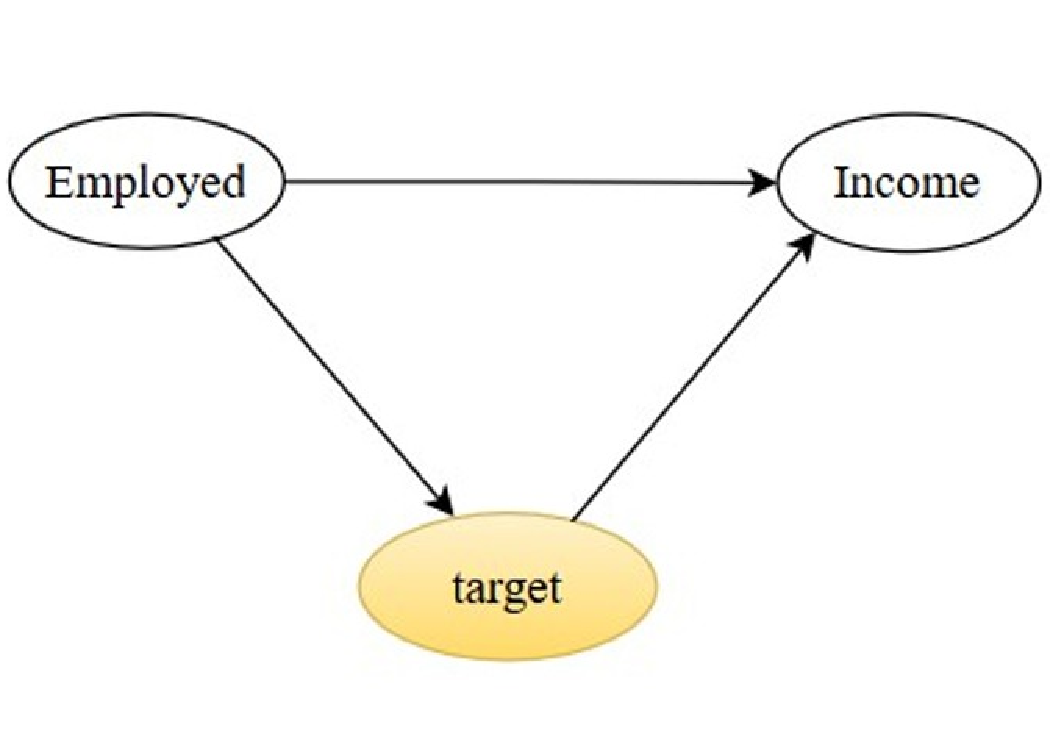
\includegraphics[width=\textwidth]{image/whatif/subnetwork/sub_au.pdf}
        \caption{Đồ thị con của Australian Credit}
        \label{fig:subnet_australian}
    \end{subfigure}
    \hfill
    % --- HÀNG 1: German Credit ---
    \begin{subfigure}[b]{0.45\textwidth}
        \centering
        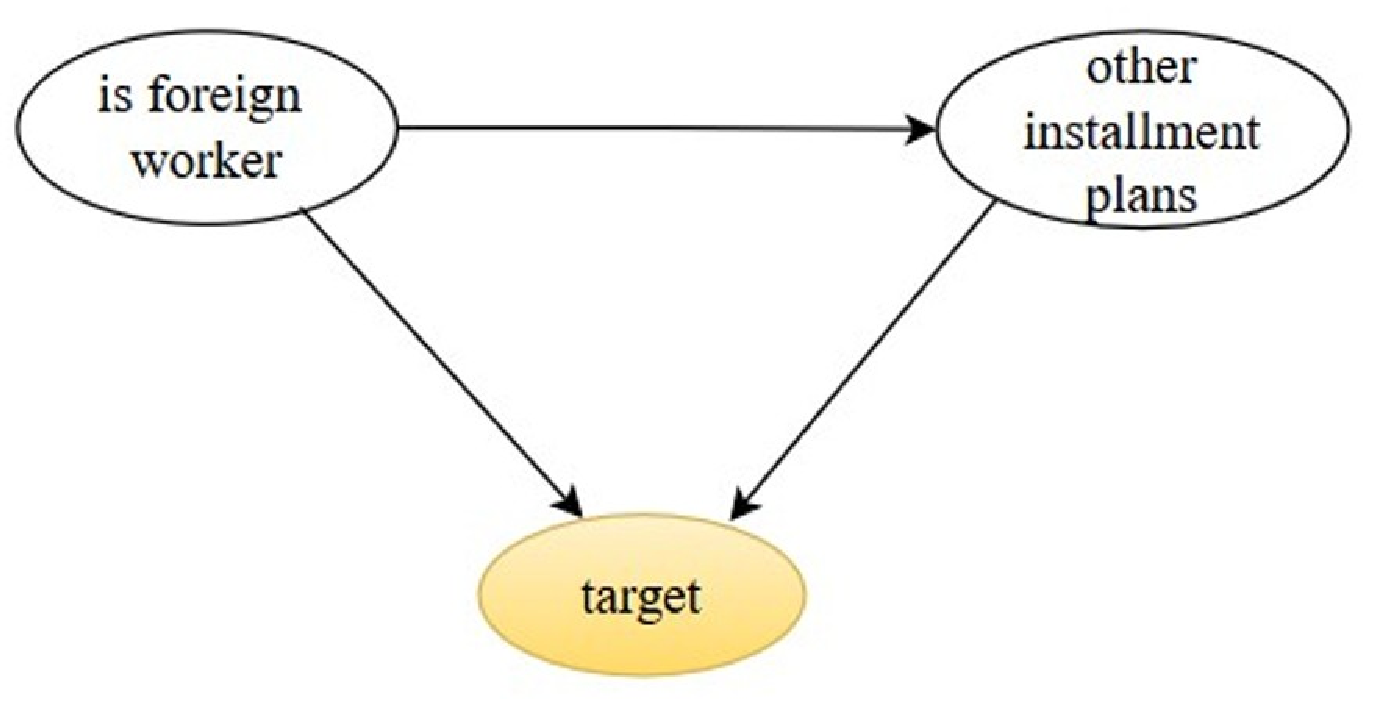
\includegraphics[width=\textwidth,
        height=0.14\textheight,
        trim=0cm 0cm 0cm 2cm,]{image/whatif/subnetwork/sub_ger.pdf}
        \caption{Đồ thị con của German Credit}
        \label{fig:subnet_german}
    \end{subfigure}
    \hfill
    \begin{subfigure}[b]{0.5\textwidth}
         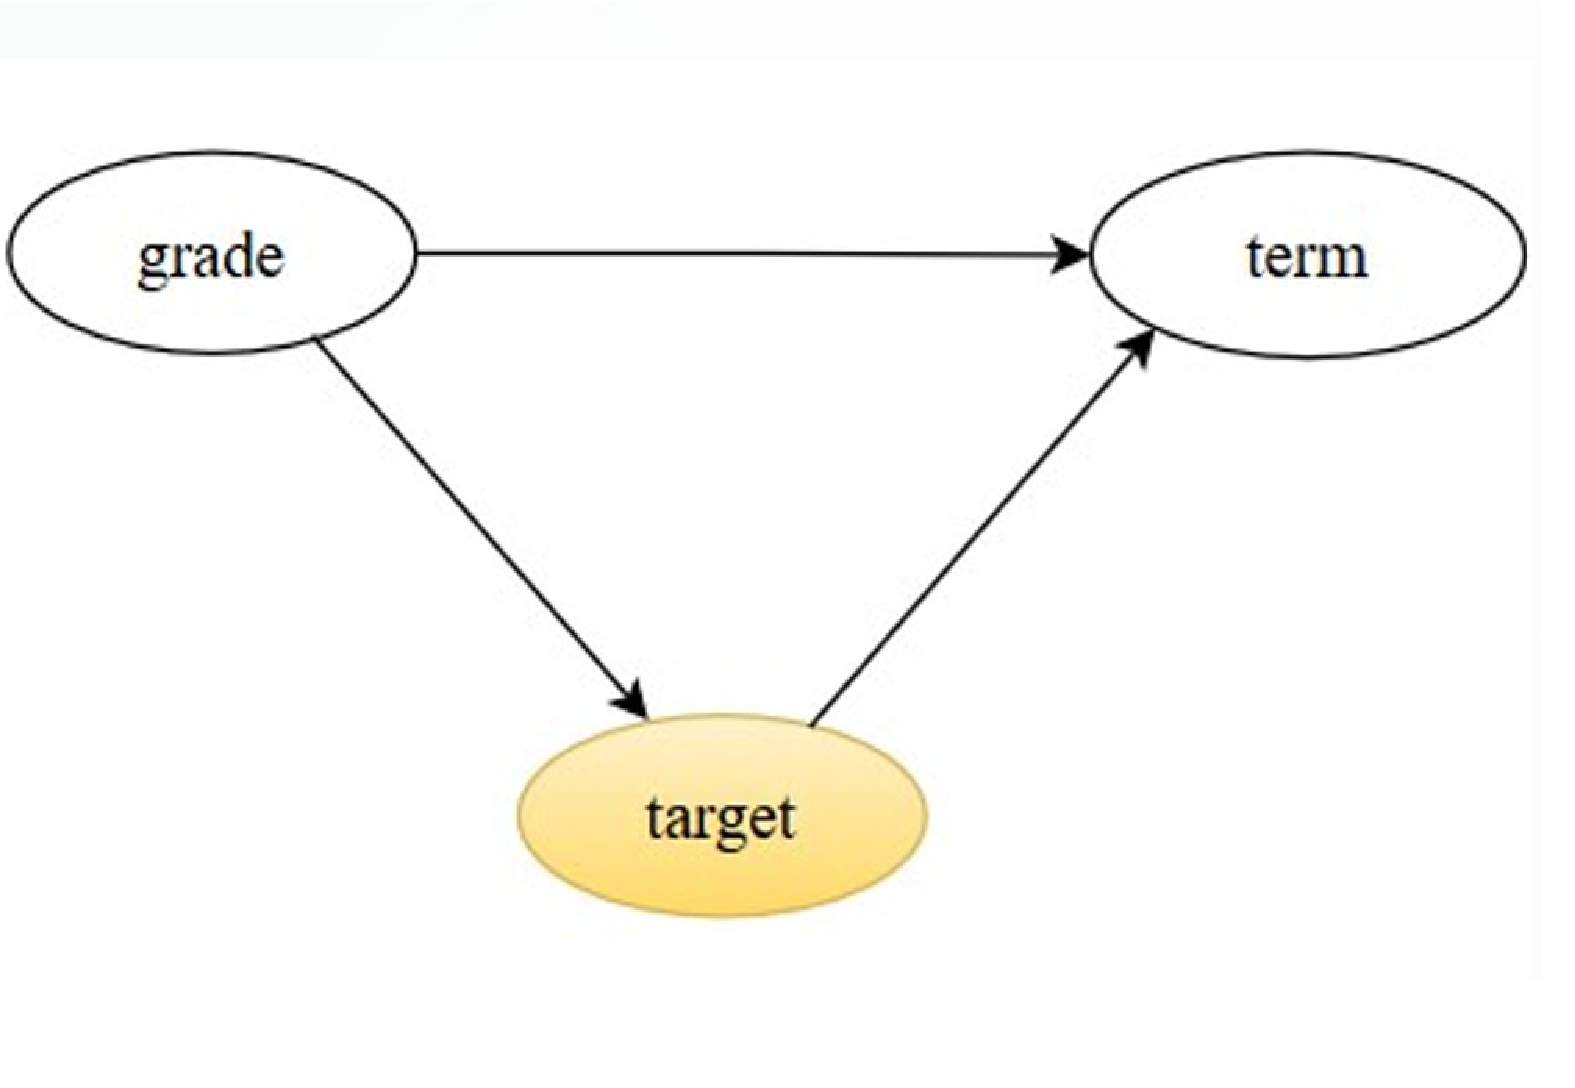
\includegraphics[width=\textwidth,
         height=0.25\textheight]{image/whatif/subnetwork/sub_lend.pdf}
        \caption{Đồ thị con của Lending Club}
        \label{fig:subnet_lendingclub}
    \end{subfigure}

    \caption{Đồ thị con của ba mạng Bayes}
    \label{fig:subnet_structures}

\end{figure}


\FloatBarrier
%%%%%%%%%%%%%%%%%%%%%%%%%%%%%%%
\begin{table}[htbp]
\centering
\caption{CPT của target theo Employed × Income --- Australian Credit}
\label{tab:cpt_australian}
\begin{tabular}{lcccccccc}
\toprule
Employed & 0 & 0 & 0 & 0 & 1 & 1 & 1 & 1 \\
Income   & 0 & 1 & 2 & 3 & 0 & 1 & 2 & 3 \\
\midrule
$P(\text{target}=1)$ & 0.7190 & 0.7474 & 0.7871 & 0.6174 & 0.2455 & 0.6606 & 0.3026 & 0.0441 \\
$P(\text{target}=0)$ & 0.2810 & 0.2526 & 0.2129 & 0.3826 & 0.7545 & 0.3394 & 0.6974 & 0.9559 \\
\bottomrule
\end{tabular}
\end{table}
\FloatBarrier

Trên Australian Credit, cấu trúc con được chọn là \texttt{Employed} (cha) - target - \texttt{Income} (con), khép vòng qua cạnh trực tiếp \texttt{Employed} $\rightarrow$ \texttt{Income} (Hình \ref{fig:subnet_australian}, Bảng \ref{tab:cpt_australian}). Quy tắc rủi ro cao nhất: chưa có việc làm và \texttt{Income} ở bin 2 cho xác suất vỡ nợ cao nhất (78.71\%). Quy tắc rủi ro thấp nhất: đang có việc làm và \texttt{Income} ở bin 3 cho xác suất thấp nhất (4.41\%) chênh lệch hơn 74 điểm phần trăm giữa hai thái cực.

\vspace{1em}
\begin{table}[htbp]
\centering
\caption{CPT của target theo is\_foreign\_worker × other\_installment\_plans --- German Credit}
\label{tab:cpt_german}
\begin{tabular}{lcccccc}
\toprule
is\_foreign\_worker & 0 & 0 & 0 & 1 & 1 & 1 \\
other\_installment\_plans & 0 & 1 & 2 & 0 & 1 & 2 \\
\midrule
$P(\text{target}=1)$ & 1.0000 & 0.6491 & 1.0000 & 0.5948 & 0.3482 & 0.7705 \\
$P(\text{target}=0)$ & 0.0000 & 0.3509 & 0.0000 & 0.4052 & 0.6518 & 0.2295 \\
\bottomrule
\end{tabular}
\end{table}


\vspace{1em}
\begin{table}[htbp]
\centering
\caption{CPT của target theo grade × term --- Lending Club}
\label{tab:cpt_lendingclub}
\begin{tabular}{lcccccccc}
\toprule
grade & 0 & 0 & 1 & 1 & 2 & 2 & 3 & 3 \\
term  & 0 & 1 & 0 & 1 & 0 & 1 & 0 & 1 \\
\midrule
$P(\text{target}=1)$ & 0.1515 & 0.3977 & 0.3528 & 0.5214 & 0.5109 & 0.6186 & 0.5645 & 0.6579 \\
$P(\text{target}=0)$ & 0.8485 & 0.6023 & 0.6472 & 0.4786 & 0.4891 & 0.3814 & 0.4355 & 0.3421 \\
\midrule
grade & 4 & 4 & 5 & 5 & 6 & 6 & & \\
term  & 0 & 1 & 0 & 1 & 0 & 1 & & \\
\midrule
$P(\text{target}=1)$ & 0.6255 & 0.6961 & 0.5829 & 0.6802 & 0.6111 & 0.6723 & & \\
$P(\text{target}=0)$ & 0.3745 & 0.3039 & 0.4171 & 0.3198 & 0.3889 & 0.3277 & & \\
\bottomrule
\end{tabular}
\end{table}


\vspace{1em}
Trên German Credit, cấu trúc con được chọn là \texttt{is\_foreign\_worker} và \texttt{other\_installment\_plans}, hai biến cha có liên kết trực tiếp với nhau, cùng khép vòng qua target (Hình \ref{fig:subnet_german}, Bảng \ref{tab:cpt_german}). Hai tổ hợp đạt xác suất vỡ nợ tuyệt đối 100\% đều rơi vào nhóm lao động nước ngoài (\texttt{is\_foreign\_worker}=0, quy ước "Yes"), dù ở hai trạng thái trái ngược của \texttt{other\_installment\_plans} ("Bank" và "none"). Quy tắc rủi ro thấp nhất là không phải lao động nước ngoài kết hợp "stores" (34.82\%).

Trên Lending Club, cấu trúc con được chọn là \texttt{grade} (cha) - target - \texttt{term} (con), khép vòng qua cạnh trực tiếp \texttt{grade} $\rightarrow$ \texttt{term} (Hình \ref{fig:subnet_lendingclub}, Bảng \ref{tab:cpt_lendingclub}). Ở mọi hạng tín dụng, kỳ hạn vay 60 tháng luôn mang xác suất vỡ nợ cao hơn kỳ hạn 36 tháng, và mức chênh lệch này khá ổn định qua các hạng (dao động 6--25 điểm phần trăm), cho thấy \texttt{term} tác động cộng dồn tương đối đều đặn lên \texttt{grade} thay vì tạo ra tương tác khuếch đại như cặp biến ở German Credit.

Tổng hợp cả hai cách tiếp cận, phương pháp persona-based phù hợp khi mục tiêu là tư vấn can thiệp cho một hồ sơ cụ thể, kết quả trực quan và dễ diễn giải bằng $\Delta P$ so với một baseline cố định, nhưng chỉ phản ánh đúng cho đúng hồ sơ neo đã chọn. Ngược lại, phương pháp subnetwork/CPT cho một bức tranh toàn cục về mọi tổ hợp trạng thái có thể xảy ra giữa hai biến có quan hệ cấu trúc trực tiếp, phù hợp để rút ra quy tắc quản trị rủi ro ở cấp độ chính sách thay vì cho một cá nhân cụ thể. Việc kết hợp cả hai cách tiếp cận, như đã thực hiện trong khóa luận, cho phép vừa phục vụ nhu cầu tư vấn cá nhân hóa vừa cung cấp cơ sở hoạch định chính sách tín dụng ở quy mô tổng thể.


\subsubsection{So sánh với LIME/SHAP}
\noindent
Với mỗi bộ dữ liệu, một khách hàng được chọn ngẫu nhiên và giải thích đồng thời bằng ba cách: LIME, SHAP, và biểu đồ diễn giải của Mạng Bayes, gán từng biến làm evidence theo đúng thứ tự các nút trong đồ thị và ghi nhận mức thay đổi xác suất hậu nghiệm sau mỗi bước.

Trên Australian Credit, khách hàng được chọn có xác suất vỡ nợ $87,6\%$, chưa có lịch sử tín dụng, chưa có việc làm, và biến \textit{Income} nằm ở bin cao nhất. Cả ba phương pháp diễn giải đều thống nhất \textit{CreditHistory} là yếu tố chi phối chính làm tăng rủi ro vỡ nợ: LIME gán $+65,4\%$, Mạng Bayes gán $+42,4\%$. Với SHAP, $\textit{CreditHistory} = 0.0$ và $\textit{Income} = 3.0$ là hai biến nằm về phía đẩy dự đoán lên cao, trong đó \textit{CreditHistory} nằm sát ranh giới quyết định $f(x) = 0.88$ — vị trí phản ánh vai trò chi phối của biến này đối với kết quả dự đoán cuối cùng. Sự đồng thuận của cả ba phương pháp về biến chi phối, dù mỗi phương pháp dựa trên cơ chế toán học khác nhau, củng cố độ tin cậy của kết luận rằng tình trạng thiếu lịch sử tín dụng là nguyên nhân chính dẫn đến đánh giá rủi ro cao đối với hồ sơ này.

Trên German Credit, khách hàng được chọn có xác suất vỡ nợ 5.3\% (Hình \ref{fig:explain_german}). Cả ba phương pháp đều thống nhất chiều tác động chung ở \texttt{other\_installment\_plans}, \texttt{secondary\_obligor}, \texttt{job} và \texttt{status\_and\_sex} (đều làm giảm rủi ro). Tuy nhiên có hai điểm bất đồng đáng chú ý. Thứ nhất, \texttt{credit\_history}: LIME không đưa biến này vào top 7 quan trọng nhất, trong khi Mạng Bayes gán $+10.6\%$ (mức tăng rủi ro lớn nhất hồ sơ) và SHAP cũng xác nhận \texttt{credit\_history} = 1.0 là đoạn hồng. Thứ hai, \texttt{housing}: LIME ($+8.0\%$) và SHAP (đoạn hồng rõ rệt cho \texttt{housing} = 0.0) đều xem đây là yếu tố làm tăng rủi ro, nhưng biến này lại hoàn toàn biến mất khỏi biểu đồ diễn giải của Mạng Bayes, tức đóng góp của nó dưới ngưỡng ghi nhận tại đúng thời điểm được thêm vào chuỗi bằng chứng tuần tự.

Trên Lending Club, khách hàng được chọn có xác suất vỡ nợ rất thấp, chỉ 3.4\%, với \texttt{debt\_settlement\_flag} ở trạng thái "không" (0), trái ngược với hồ sơ rủi ro cực trị đã phân tích trước đó. LIME vẫn xếp \texttt{debt\_settlement\_flag} $\leq$ 0.00 là yếu tố làm giảm rủi ro mạnh nhất ($-21.4\%$), trong khi Mạng Bayes lại cho thấy vai trò của biến này gần như không đáng kể ($-0.4\%$) và thay vào đó xác định \texttt{int\_rate} = 0 mới là yếu tố chi phối chính ($-28.1\%$), theo sau là \texttt{grade} = 0 ($-11.1\%$); SHAP cũng đồng thuận với Mạng Bayes khi \texttt{int\_rate} = 0.0 chiếm phần lớn đoạn màu xanh (giảm rủi ro), còn \texttt{debt\_settlement\_flag} không đủ ngưỡng để xuất hiện trong biểu đồ. Sự bất đối xứng này giữa hai trạng thái của \texttt{debt\_settlement\_flag} rất đáng chú ý: khi ở trạng thái hiếm gặp (= 1, đang trong chương trình tái cơ cấu nợ), biến này gần như quyết định tuyệt đối kết quả như đã ghi nhận ở hồ sơ trước (Mạng Bayes $+54.6\%$); nhưng khi ở trạng thái phổ biến (= 0, không tái cơ cấu), nó chỉ mang rất ít thông tin bổ sung so với những gì \texttt{int\_rate} và \texttt{grade} đã thể hiện, vì phần lớn khách hàng vốn dĩ đã ở trạng thái này. LIME dường như không phân biệt được sự bất đối xứng này vì phương pháp xấp xỉ tuyến tính cục bộ gán trọng số dựa trên mức độ nhiễu loạn xung quanh điểm dữ liệu chứ không phản ánh đúng phân phối thực của biến trong toàn bộ tập dữ liệu.

Tổng hợp cả ba bộ dữ liệu, cả ba phương pháp nhìn chung thống nhất về chiều tác động và biến chi phối chính của từng hồ sơ, cho thấy cấu trúc nhân quả mà mạng Bayes học được không mâu thuẫn với các phép xấp xỉ hậu kiểm phổ biến. Tuy nhiên, độ lớn đóng góp cụ thể (trong trường hợp German Credit là cả chiều tác động của một vài biến) không đồng nhất giữa ba phương pháp, đặc biệt khi bảng CPT liên quan đến dữ liệu thưa hoặc khi ảnh hưởng của một biến phụ thuộc mạnh vào các biến khác đã được cố định trước đó trong chuỗi lan truyền bằng chứng. Ngoài ra, thứ tự trình bày các biến trong Mạng Bayes phụ thuộc vào thứ tự các nút trong đồ thị chứ không tự động sắp xếp theo độ lớn đóng góp như LIME hay SHAP, nên một số biến quan trọng có thể xuất hiện ở vị trí giữa biểu đồ thay vì đầu bảng. Đây là một khác biệt về cách trình bày cần lưu ý khi so sánh trực tiếp ba phương pháp, hơn là một khác biệt về bản chất suy luận.

\begin{figure}[H]
\centering
{\small \textbf{Xác suất dự đoán}: Is default ~=~0.8762, No default~=~0.1238}\\[0.3em]
\vspace{0.8em}
\begin{subfigure}[b]{0.9\textwidth}
    \centering
    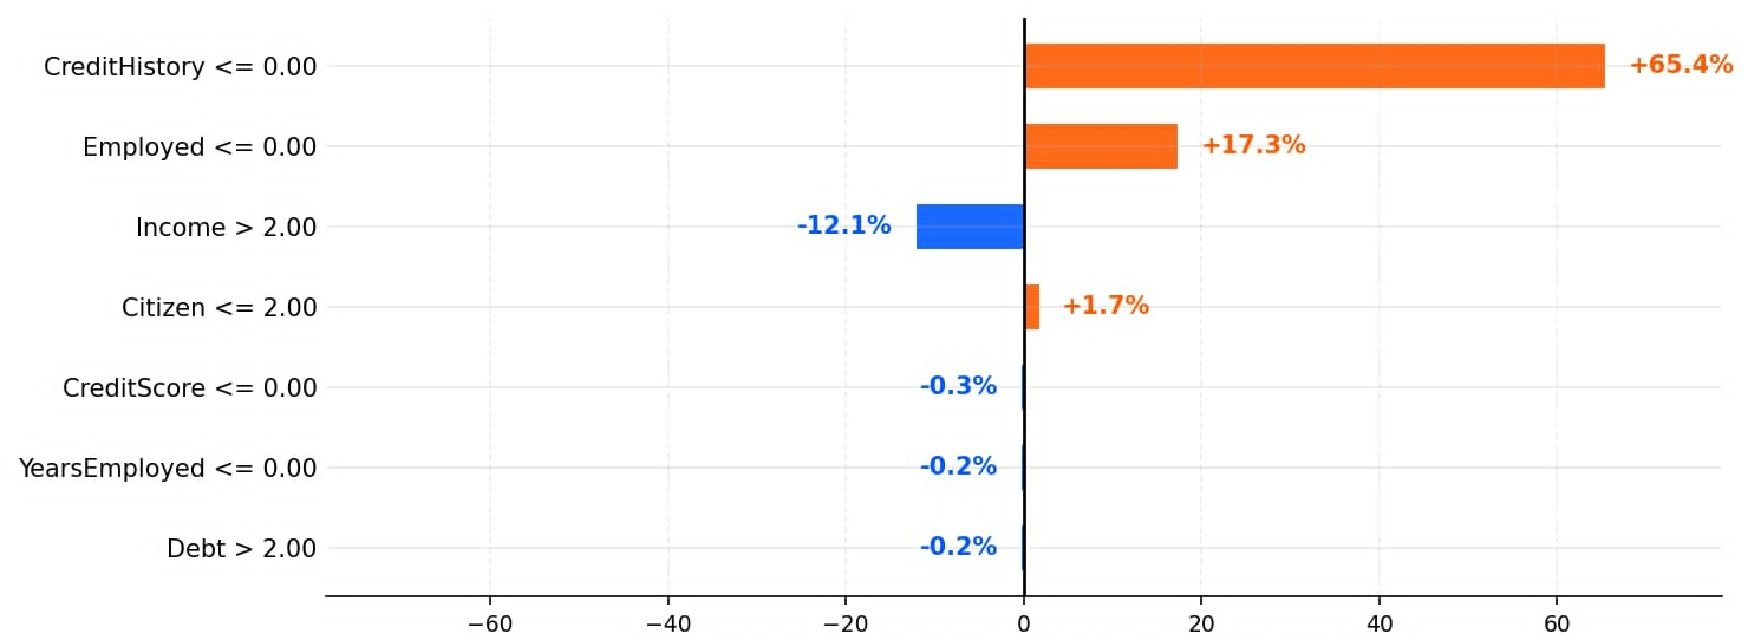
\includegraphics[width=\textwidth]{image/limeshap/au_lime_1.pdf}
    \caption{LIME}
    \label{fig:au_lime}
\end{subfigure}
\vspace{0.8em}
\begin{subfigure}[b]{0.7\textwidth}
    \centering
    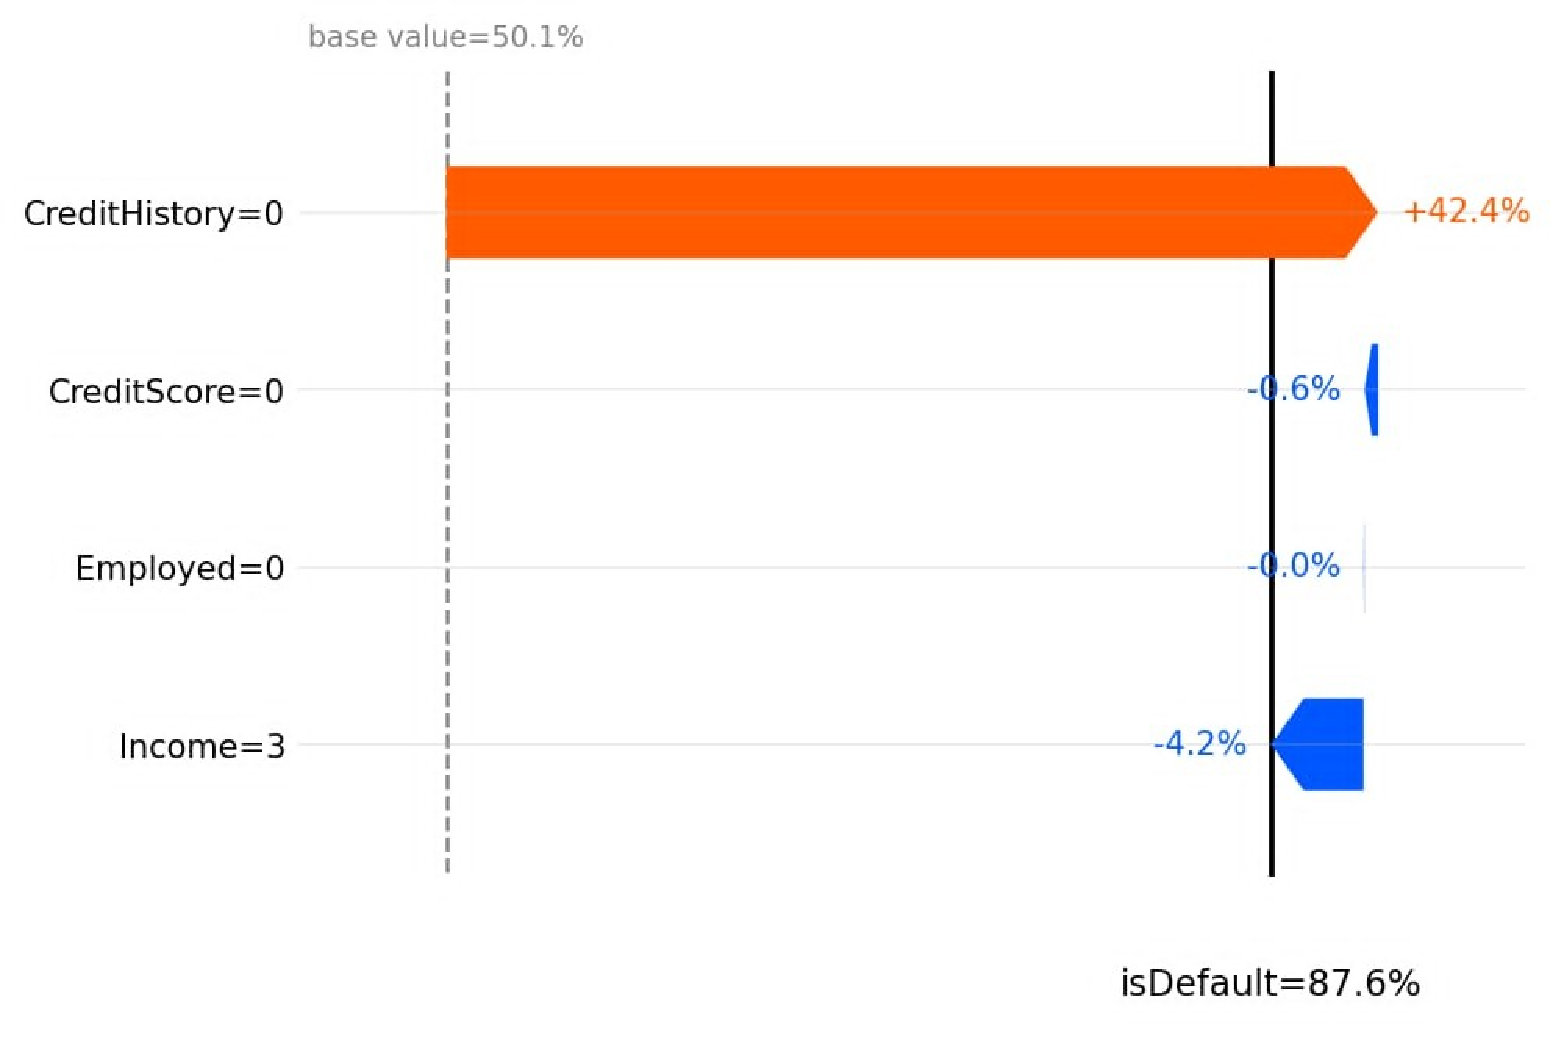
\includegraphics[width=\textwidth]{image/limeshap/au_lime_2.pdf}
    \caption{Mạng Bayes}
    \label{fig:au_waterfall}
\end{subfigure}
\vspace{0.8em}
\begin{subfigure}[b]{1.1\textwidth}
    \centering
    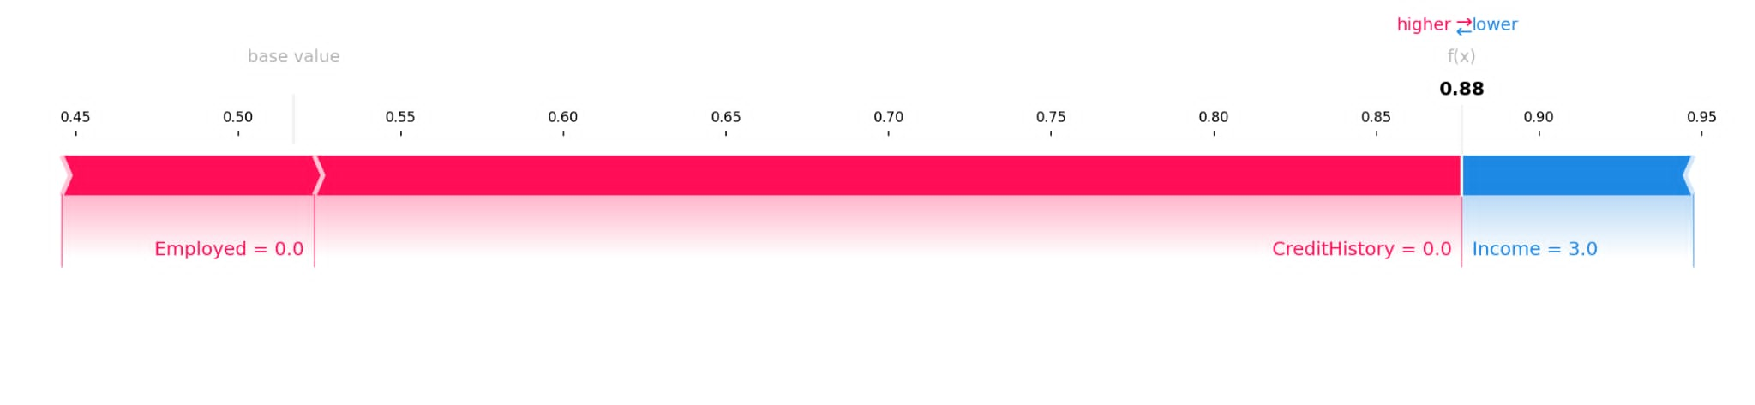
\includegraphics[width=\textwidth,
        height=0.18\textheight,
        trim=1cm 2cm 0cm 0cm,
        clip]{image/limeshap/au_shap.pdf}
    \caption{SHAP}
    \label{fig:au_shap}
\end{subfigure}
\caption{So sánh ba phương pháp giải thích cục bộ cho một hồ sơ khách hàng ngẫu nhiên --- Australian Credit}
\label{fig:explain_australian}
\end{figure}

\begin{figure}[htbp]
\centering
{\small \textbf{Xác suất dự đoán}: Is default ~=~0.0526, No default~=~0.9474}\\[0.3em]

\vspace{0.8em}
\begin{subfigure}[b]{1\textwidth}
    \centering
    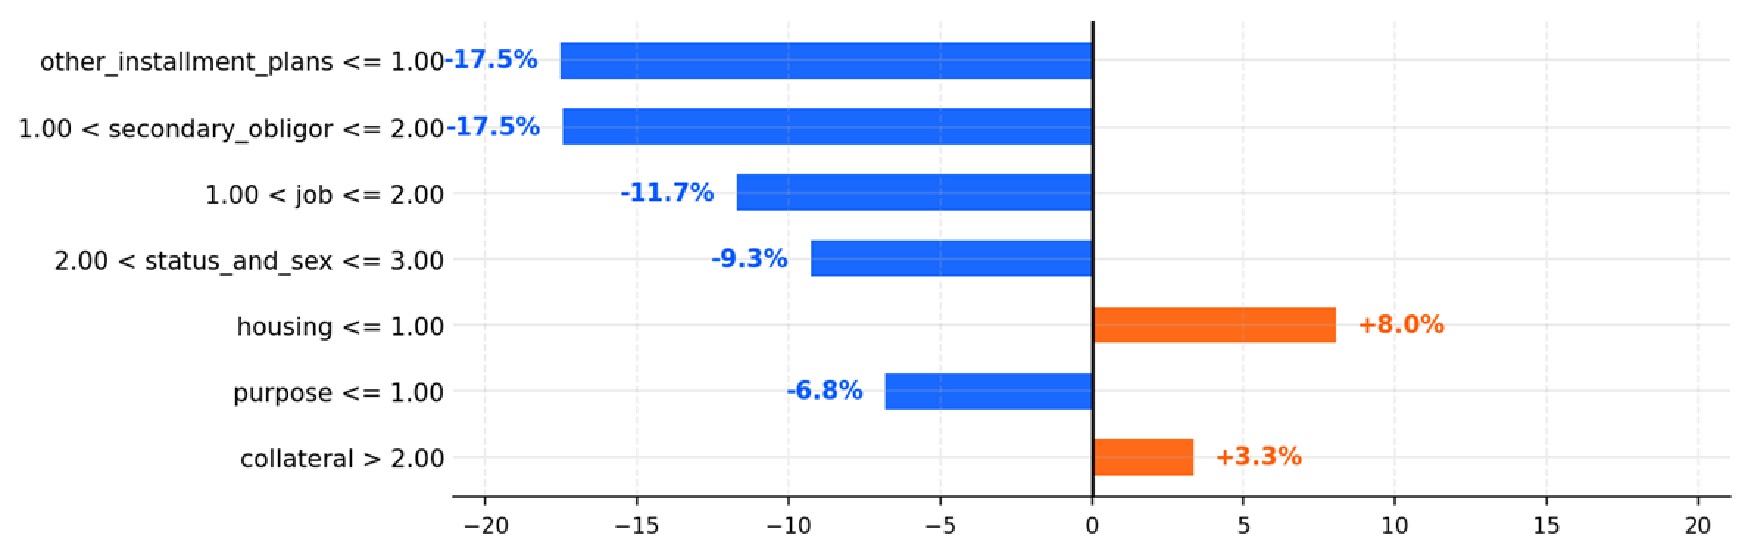
\includegraphics[width=\textwidth]{image/limeshap/ger_lime_1.pdf}
    \caption{LIME}
    \label{fig:ger_lime}
\end{subfigure}
\vspace{0.8em}
\begin{subfigure}[b]{0.8\textwidth}
    \centering
    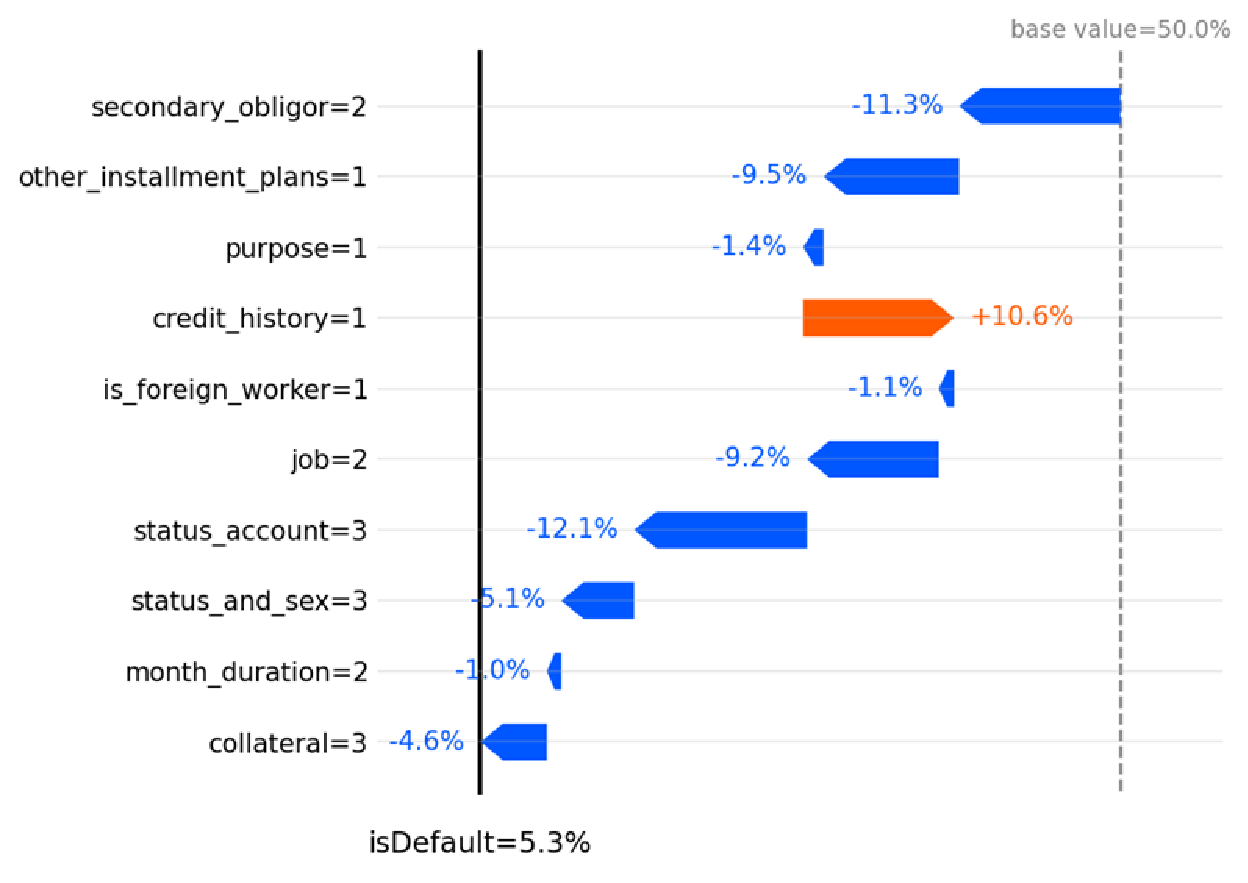
\includegraphics[width=\textwidth]{image/limeshap/ger_lime_2.pdf}
    \caption{Mạng Bayes}
    \label{fig:ger_waterfall}
\end{subfigure}
\vspace{0.8em}
\begin{subfigure}[b]{1.1\textwidth}
    \centering
    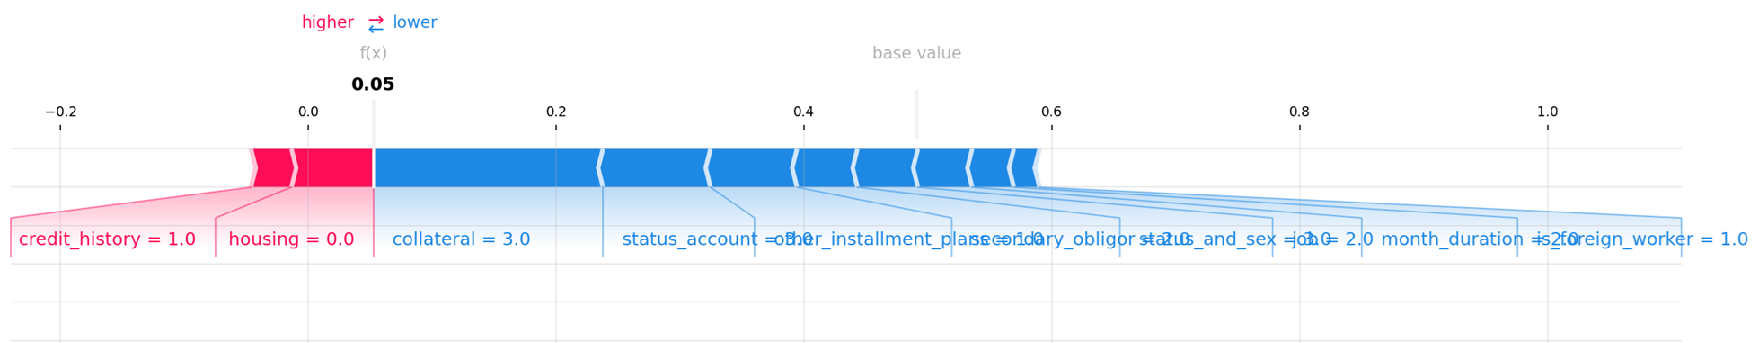
\includegraphics[width=\textwidth]{image/limeshap/ger_shap.pdf}
    \caption{SHAP}
    \label{fig:ger_shap}
\end{subfigure}
\caption{So sánh ba phương pháp giải thích cục bộ cho một hồ sơ khách hàng ngẫu nhiên --- German Credit}
\label{fig:explain_german}
\end{figure}

\begin{figure}[htbp]
\centering
{\small \textbf{Xác suất dự đoán}: Is default ~=~0.0338, No default~=~0.9662 }\\[0.3em]

\vspace{0.8em}
\begin{subfigure}[b]{0.9\textwidth}
    \centering
    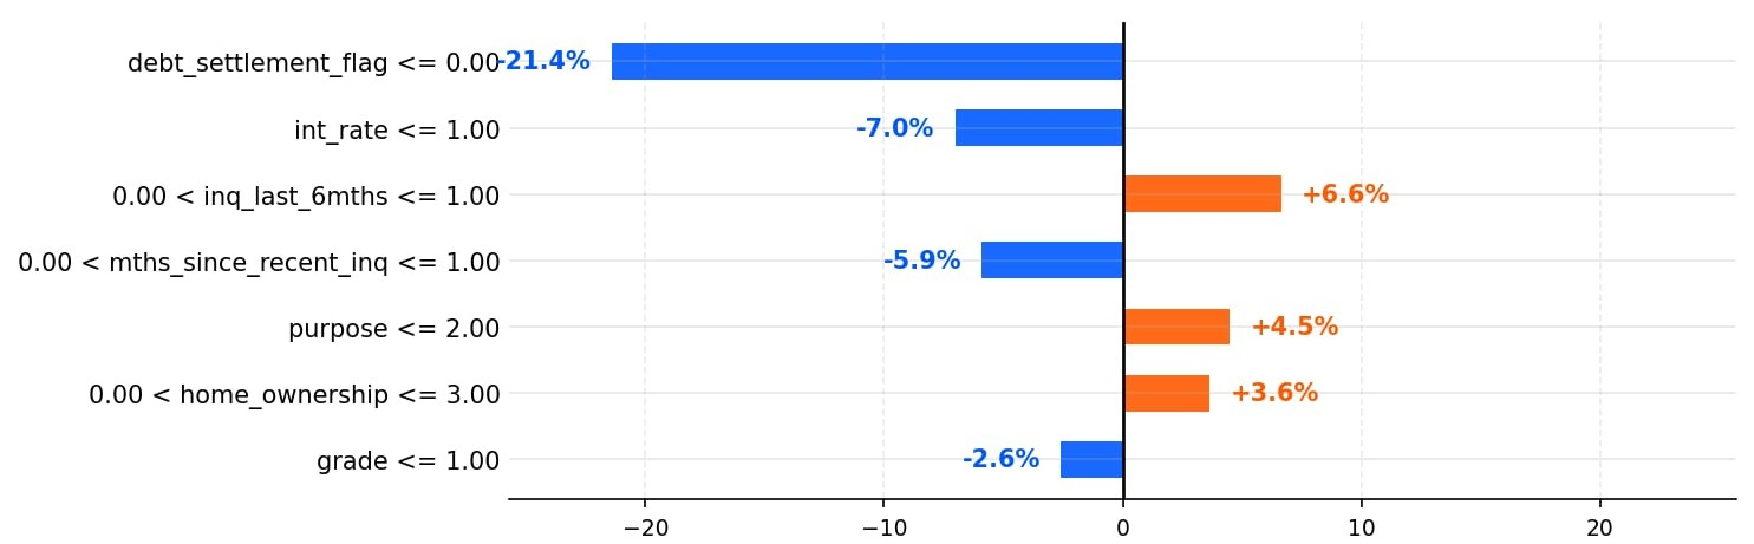
\includegraphics[width=\textwidth]{image/limeshap/lend_lime_1.pdf}
    \caption{LIME}
    \label{fig:lend_lime}
\end{subfigure}
\vspace{0.8em}
\begin{subfigure}[b]{0.8\textwidth}
    \centering
    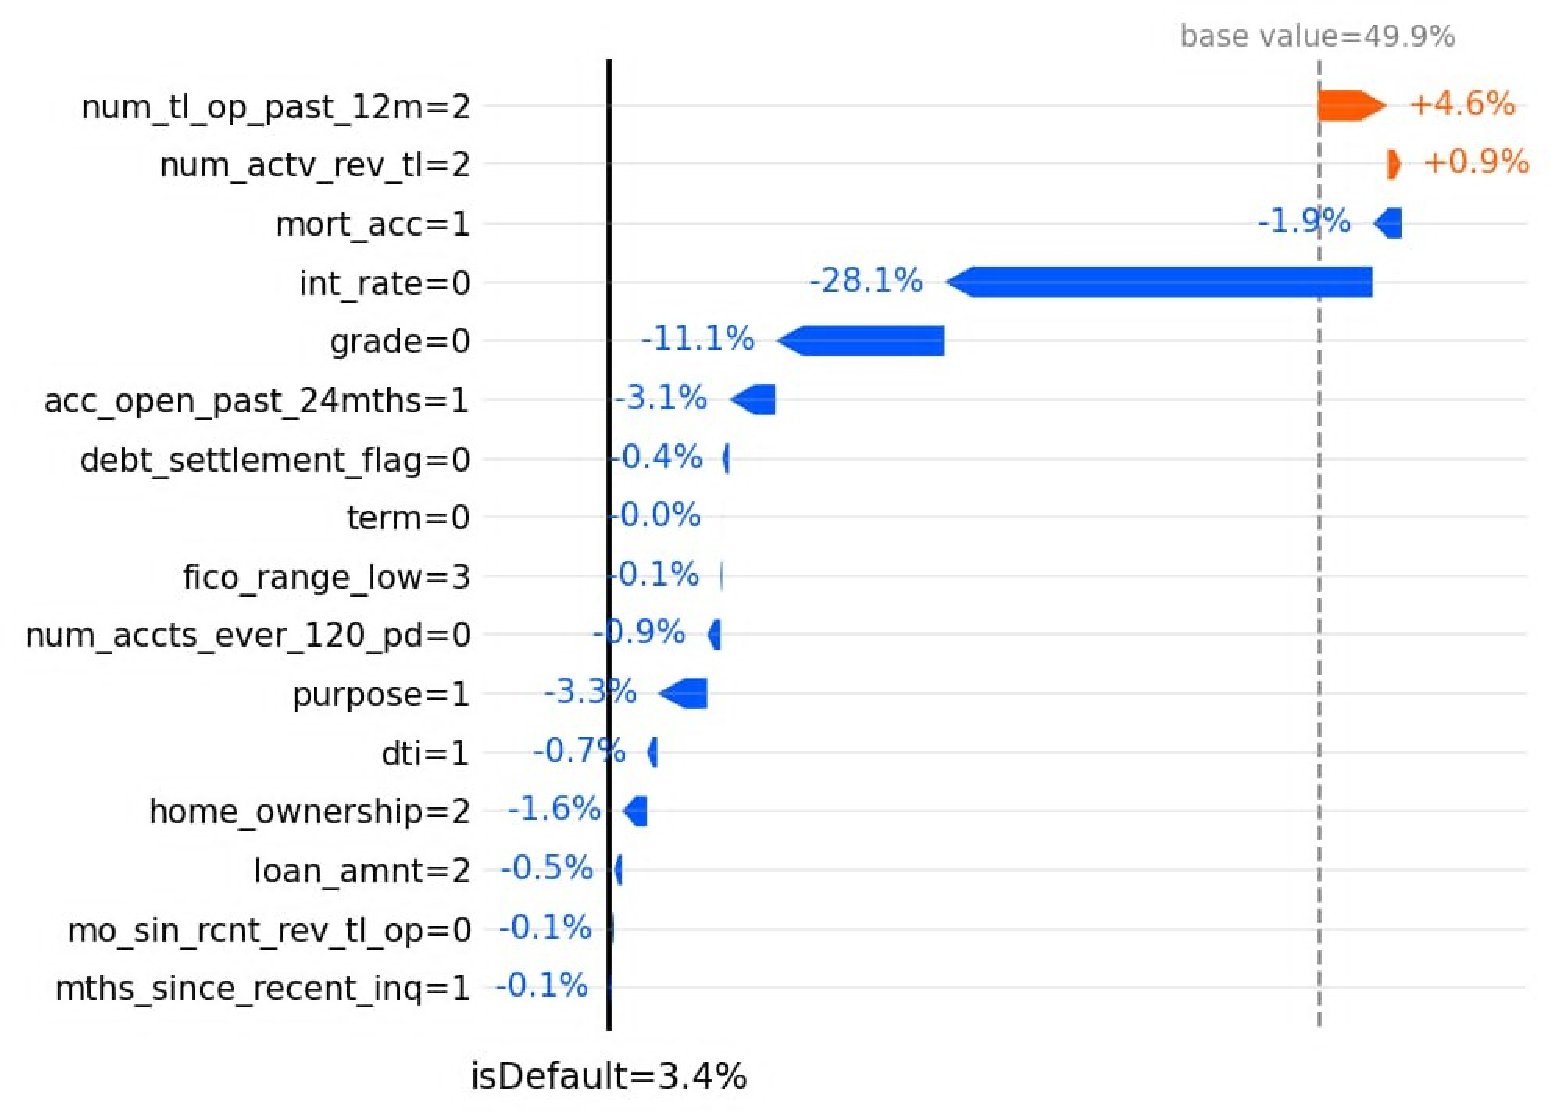
\includegraphics[width=\textwidth]{image/limeshap/lend_lime_2.pdf}
    \caption{Mạng Bayes}
    \label{fig:lend_waterfall}
\end{subfigure}
\vspace{0.8em}
\begin{subfigure}[b]{1.1\textwidth}
    \centering
    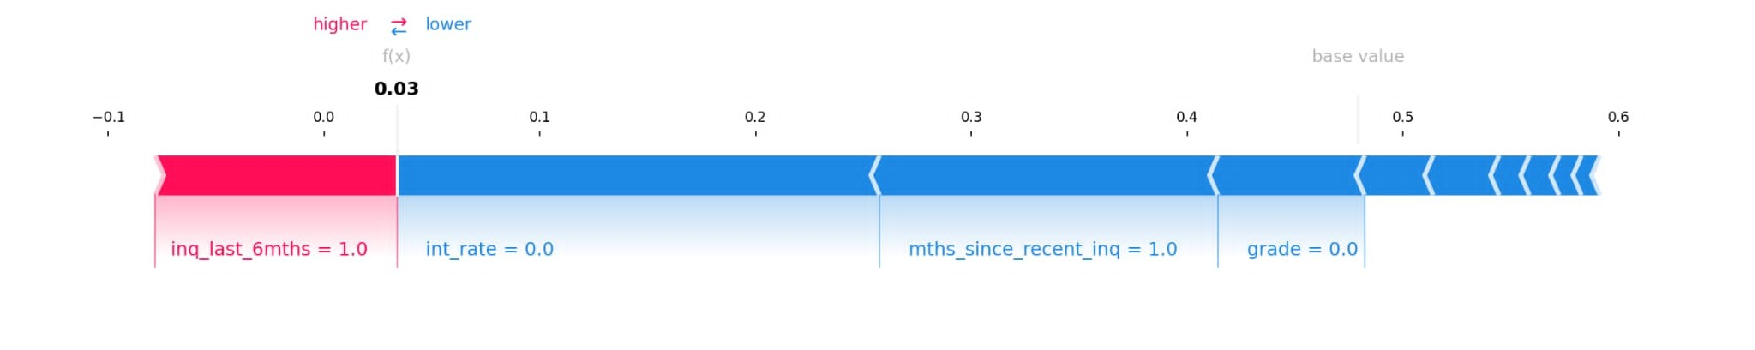
\includegraphics[width=\textwidth,
        height=0.18\textheight,
        trim=1cm 1cm 0cm 0cm,
        clip]{image/limeshap/lend_shap.pdf}
    \caption{SHAP}
    \label{fig:lend_shap}
\end{subfigure}
\caption{So sánh ba phương pháp giải thích cục bộ cho một hồ sơ khách hàng ngẫu nhiên --- Lending Club}
\label{fig:explain_lendingclub}
\end{figure}

\FloatBarrier
